%l Copyright all rights reserved, Charles Severance 2010, 2011

% TODO: No more double quotes 

% TODO Bill Thompson

% TODO Joseph Reports and non-funding
% TODO Sakai Principles from January 2006 blog posts

% 2004-11-01-05 JISC Meeting Kassam Stadium Oxford - With Rob's Family - Ares Birthday.

% 2007-10-06 Conference in Ann Arbor with Ties and Adrian

\documentclass[12pt]{book}
\usepackage[size=journal,gutter=0.7in,trim,bleed]{createspace}

% https://github.com/aginiewicz/createspace/wiki/documentation

\usepackage{pslatex}
\usepackage{url}
\usepackage{fancyhdr}
\usepackage{graphicx}
\usepackage{amsmath, amsthm, amssymb}
\usepackage{exercise}
\usepackage{makeidx}
\usepackage{setspace}
\usepackage{upquote}
\usepackage{textcomp}
\usepackage{caption}

\newcommand{\thetitle}{Sakai: Free as in Freedom (Beta)}
\newcommand{\theversion}{0.8.draft}

\hyphenation{NEES-Grid pro-jects}

\makeindex

\begin{document}

\frontmatter

\thispagestyle{empty}

%--title page--------------------------------------------------
\pagebreak
\thispagestyle{empty}

\begin{flushright}
\vspace*{2.0in}

\begin{spacing}{3}
{\huge Sakai: Free as in Freedom (Alpha)}\\
{\Large A Retrospective Diary}
\end{spacing}

\vspace{0.25in}

Version \theversion

\vspace{0.5in}


{\Large
Charles Severance\\
}


\vspace{2.25in}


\end{flushright}


%--copyright--------------------------------------------------
\pagebreak
\thispagestyle{empty}

{\small
Copyright \copyright 2011- All Rights Reserved, Charles Severance.

% ISBN-13: 978-1461166290

% ISBN-10: 1461166292

% CreateSpace Title: 3609835

Front Cover Photography: Town Square Photo, Mason MI

Back Cover Photography: HJ Seeley

Sakaiger Art: www.sakaiger.com

Draft 0.0.1 Printing: January 2011, Michigan Library Espresso Book Machine

Draft 0.0.2 Printing: March 2011, Michigan Library Espresso Book Machine

First Printing (Alpha 0.7.1) : May 2011, Amazon CreateSpace

Second Printing (Alpha 0.7.2) : January 2012, Amazon CreateSpace

} % end small

\chapter*{Preface}

Writing software that supports teaching, learning and collaboration is
far more than just a job.  Since teaching and learning are some of
the most fundamental human activities, we all have a vested interest
in teaching and learning software.  Discussions about the design of
teaching and learning software can evoke passions from virtually
everyone involved in the process.   Passions run high and the
stakes are high.  On most college campuses, the software to
support teaching and learning (Blackboard, Moodle, Sakai, etc.)
is used more often than any other campus software.   Student and
teacher lives revolve around the software.  A significant outage
of a course management system in the last few weeks of class is
likely to produce howls of anger from students, teachers,
and administrators alike.\\
 \\
Building an open source product and community around the Sakai
Learning Management System was far from a mere technical activity.
This book is about that journey of
making open source software
and deriving and changing the rules as to how we would make that
software as we went along.  It is about software developers,
managers, designers, and end users all dropped into a crucible
and put under pressure to make something great and do so
in record time.\\
 \\
Charles Severance\\
www.dr-chuck.com\\
Ann Arbor, MI, USA\\
May 8, 2011\\
 \\
Charles Severance is a
Clinical Associate Professor
at the University of Michigan School of Information.

\section*{About the Book}

My intention in writing this book is to give a first-person
account of the effort and passion that goes into an open
source project. I think that society oversimplifies open
source as a bunch of altruistic nerds working in their basements
around the world.   Open source projects are
often as complex, exciting, rich, and stressful as commercial
efforts.  In some ways, open source is more complex
than commercial activities because there are so many moving
parts and there is no real ``boss'' to make final decisions.

Decisions are made based on long discussions that search
for the group's consensus position, often with strong
passions on all sides. I hope to capture
some of the emotion behind the scenes in the Sakai project
that was launched in 2004.

Many people participated in the leadership of Sakai and they
have their own stories.  This book presents my story and perspective
as chief architect in the project.  Others
are likely to have different perspectives on the events
I describe.

The first edition of the book is an ``Alpha'' version of the
book.  It will have mistakes, typographical errors, and gaps
in the arc of the story line.  But I needed to deliver it
on time so I released an Alpha version to make
my own self-imposed
deadline (like we did in Sakai several times).

You can find errata, links to supporting materials, images,
videos, and a full timeline of my involvement in Sakai at:

\url{http://www.dr-chuck.com/sakai-book/}

You can also find me on Twitter as @drchuck.  You can
add '@drchuck' to a tweet and I will see it.  Feel free
to send me comments, reviews, typos, factual errors, or
any other reaction as you read the book.

Since it takes a village to find and fix my mistakes, I
need to thank all of the many people who looked at early versions
of the book including:

Brad Wheeler, Glenn Golden, Seth Theriault, Anthony Whyte, Rob Lowden, Lance Speelmon, Craig Counterman, Lois Brooks, Shoji Kajita, Vivie Sinou, Ian Dolphin, John Norman, Ian Boston, Robert Crouchley, Adrian Fish, RJ (Robert) Allan, Stephen Marquard, David Horwitz, Alan Berg, David Barroso, Alexandre Ballest\'e, Joseph Hardin, Susan Hardin, Mark Norton, Greg Gay, Steve Swinsburg, Joel Greenberg, John Williams, Shawn Mehan, Beth Kirschner, John Leasia, Noah Botimer, Jim Eng, David Haines, Gonzalo Silverio, Matthew Jones, Marc Alier, Eva de Lera, Francesc Santanach Delisau, Llu\'is Vicent, Pablo Casado Arias, Megan May, Tom Finholt, Jan Posten Day, John Fontaine, George Kroner, Erin Knight, Nathan Gandomi, Andrew Krumm, Nicola Monat-Jacobs, Sam Ottenhoff, Scott Siddall, Kazou Yana, Russell Severance, Richard Wiggins, Judy Matthews, and Mary Miles.

The book was written on a Macintosh using the ``vi'' editor and
formatted using LaTeX.  Early drafts of the book were printed
on the Espresso Book Machine at the University of Michigan Library
with help from Terri Geitgy.

\tableofcontents

\mainmatter

\chapter{Before Sakai}

I have been developing computer software since the 1970's.  While
technology and connectivity have
improved greatly since then, in a sense there has been little change
in why I love to write software.  From the beginning I loved
to write software that would surprise and delight the users of
that software.  The more people who found the software
to be helpful, the happier I was.   For someone who was a nearly
invisible nerd through high school, it was pretty exciting to have
an audience of users that waited anxiously for me to announce
the next feature to be developed and released.  Finally, I mattered
to a bunch of people --- even if they did not know who I was.  Even if
I was not so cool as a person, the software I produced was pretty cool.

For those of us close to the emerging Internet and World-Wide-Web
between 1985 and 1995, it seemed as though we needed to
educate everyone so they could be part of the growing worldwide
community connected by the network.

In 1994, East Lansing, Michigan was one of the first communities
in the country to rollout high speed 10 Megabit per second cable
modems.  I helped set up the connection between Michigan State
University and the TCI Cable network infrastructure.   Based on the
friendships that were developed during that project, I was asked
to co-host a talk show about the Internet with my good friend
and fellow Michigan State employee Richard Wiggins.  TCI Cable
would produce the program with John Liskey as the Executive Producer
and Amy Leahey as the Producer and Director.  The purpose of
the program was to use TCI Cable modems
on our show and regularly remind our viewers how much
faster \emph{our} connection was when compared to their measly
56 Kilobit per second telephone-based modems.

The Internet:TCI program was produced monthly in East Lansing
and tapes were shipped to TCI Cable stations around the
country to be aired on
their ``Local Origination'' channel.   At its peak, Internet:TCI
was aired in about 15 markets including Chicago, San Francisco,
and others.   The program pre-dated any other technology program
airing nationally.  We won a number of regional and national awards
for programming produced by the cable industry in 1996.

Internet:TCI had a brief moment in the sun because by 1996 it
was clear that the Internet and World-Wide-Web were big
business.  Well-financed national programs like TechTV were quickly
produced and delivered daily or weekly via satellite.  Also in the late
1990's there was a lot of consolidation and horse-trading in the cable
industry.   Our show moved from TCI Cable to MediaOne and then to
AT\&T Cable Television.  In each transition, we lost momentum
and other programming in the market made a talk show
with two middle-aged geeks talking about computer technology pretty much
irrelevant.  John Liskey, our long-time executive producer and
cheerleader, convinced TechTV to take a look at our audition
tape in 2003 to see if we could do a few pieces now and then
for one of their programs.  But by then even
TechTV had decided that smart geeks
were no longer relevant in a market increasingly interested in
attracting teenagers by doing video game previews.

Even though the Internet:TCI program did not result in a television
career for me, it did give me an excellent excuse to interview
pretty much anyone in the emerging Internet field.   Back in the mid-1990s
when things were just getting started, everyone would talk to you.
We interviewed Tim Berners-Lee, Richard Stallman, Jeff Bezos, and many
others.  Since both Rich and I were technologists before we were
journalists, our interviews often tried to get the interviewees to look
forward into the future and share their visions of where things might go.

In one interview with James Wells of the RealAudio (now Real Networks)
company, he posited that someday we would be using the Internet to
teach courses using streaming audio and 28 Kilobits per second modems.
This seemed like a great idea to me and I set about spending my spare
time at Michigan State University trying to cobble enough technology
together to let me stream audio (and later video) along with images taken
from PowerPoint slides to remote students over the Internet.  I built
a bit of software called Sync-O-Matic-3000 that helped
blend the audio, video, and slides into a single online lecture.
The software was named after a Saturday Night Live skit called
``Bass-O-Matic'' that aired on April 17, 1976.

Once I had Sync-O-Matic working in 1998, I created a new course at
Michigan State University called ``EGR124: Internet and Technology''
that would be taught online with recorded streaming lectures.
I saw the students in-person once per semester when I scheduled
an in-class midterm exam.

I tried to commercialize Sync-O-Matic in the late 1990's but was
unsuccessful.  In my inexperience, I failed to realize that venture
capitalists do not pay money for good ideas.  Instead they wanted
ideas that already have customers and a revenue stream.  I ended
up in a bit of a tussle with the Michigan State University technology
leadership as to ``who owned Sync-O-Matic.''  Once I tried to find
a buyer for the product, they decided it must be valuable and then later
when I wanted to stop trying to sell it and I decided to give it away, they told
me it belonged to them:  that they would decide how to best maximize
the profit around Sync-O-Matic and so took control of the program away
from me.

Even though I was not successful selling Sync-O-Matic, I had
given a number of presentations at academic conferences and
had met a number of people in academia that liked the idea.

In the fall of 1998, I gave a talk at San Diego State University
about Sync-O-Matic and was approached by the University of Michigan
and asked if I would come to work for them.  I had seventeen years
of seniority at Michigan State University and was eight years away
from early retirement.  But the lure of being able to pursue
my dream of building technology for teaching and learning in a
freer and more supportive environment led me to join the University
of Michigan in mid-1999 as part of the Media Union.

My new boss at the Media Union was Barbara O'Keefe.
Barbara was the director of the Media Union and seemed to have been
given plenty of resources by
the university administration.  Barbara saw our competition as
MIT Media Lab.  When I started my job, she told me
to use whatever resources I needed so long as I did
something impressive.

Almost immediately, I found out that some University
of Michigan physicists were trying to use my Sync-O-Matic software
to record some lectures at the CERN High-Energy Physics Laboratory.
They handed me a credit card, told me to buy whatever I needed,
and I got on a plane to CERN to help them out.
If my first two months were any indication, this new job
was going to be a lot more fun!

Since there was still disagreement as to who owned the source code to
Sync-O-Matic, I decided to build a whole new lecture capture system
using the Apple Macintosh and QuickTime technology instead of the RealMedia
and Windows technology I used for Sync-O-Matic.  I quickly picked
up the Macintosh programming environment and by early 2000,
had a working prototype of my next generation of lecture capture
technology which I called ClipBoard-2000.

ClipBoard was far superior to Sync-O-Matic in every way.  In ClipBoard,
there was a single desktop application that recorded audio, video,
screen scribbling, text annotations, and cursor animation.
And it produced a single multi-track QuickTime file instead of
the hundreds of interlinked web pages that Sync-O-Matic produced
for an online lecture.  Early in 2000, I even visited Apple and
demonstrated ClipBoard.  I wanted to give ClipBoard to Apple so they could
make it part of their operating system.  Back at the University
of Michigan another developer was assigned to work on a Windows
version of ClipBoard.

Then in the summer of 2000, things got a little scary.
Barbara left the University of Michigan to become the
Dean of Communication Arts and Sciences at
Northwestern University and there was talk that the Media Union
needed to ``settle down'' and stop having so much fun (i.e. stop
spending so much money).  Since the College of Engineering had
been paying half my salary since I was hired, they asked me to
teach their sophomore class in C++ in the fall of 2000.  It started
to look like I would have very little time to pursue building
any teaching and learning software going forward.

At some point, I had coffee with my friend Bryan Holland
and told him about my concerns regarding my position at
the University of Michigan.
Bryan and I had worked together at Michigan State University and
he was now the Chief Technology Officer for Strategic Interactive.
Strategic Interactive was a startup formed in 1997 focusing on
building teaching and learning technology and content delivered over the
Internet.

Bryan told me about a secret project in Microsoft called ``Microsoft
Learning Technology'' (or MLT) where Microsoft was going to
extend Microsoft Exchange to become an extensible learning
management system and Strategic Interactive was to be one of
the earliest preferred partners on the project.  Bryan said
that my lecture capture technology would be the perfect
first plug-in for MLT if we could get started quickly.  I
would have to rewrite my technology one more time using
Windows Media, but I figured that with the experience of
building Sync-O-Matic and ClipBoard, it would not take much time
at all and I would be able to make a better product
with tight integration with the MLT servers.

So in October, I quietly agreed to join Strategic Interactive
in January 2001.  But the semester had already started and
I was teaching EECS280 at the University of Michigan with Jim Eng.
This was my first teaching experience at the University of Michigan, and
I was nervous about teaching a course with 400 students
in a single lecture hall.
Thankfully Jim was an expert in all the
ins and outs of teaching at the University of Michigan College of
Engineering and we got through the semester without any major
mistakes.   As the semester progressed and the stress level dropped,
I really started to enjoy the class.

I was using my ClipBoard software to record
my lectures and had developed the server version of ClipBoard
that would automatically upload and transcode my
recorded lectures into various formats for streaming.  I would
push a button in ClipBoard on my laptop at the end of
the lecture, and by the time I walked back to my office, the
materials would be automatically uploaded to the web.

The course went so well that one of our students invited
Bjarne Stroustrup (the inventor of the C++ language)
to give a guest lecture.
We moved Bjarne's lecture to a large theater and
invited anyone in the College of Engineering to attend and
had a book signing of the hardcover edition of Bjarne's book.

By the end of the semester, it was one of my favorite teaching
experiences and things were really looking up for me at the
University of Michigan.  But since I had made the commitment
to go to Strategic Interactive, I left the University and
went to Strategic Interactive in January of 2001.

After I had been at Strategic Interactive for about two weeks,
I was told that Microsoft had cancelled the Microsoft
Learning Technology (MLT) effort.  They had just pulled the plug.
This was not good as I was a rather expensive employee
and if there was no high-revenue project for me to work on,
I felt that things might become uncomfortable pretty quickly.

In February 2001, Strategic Interactive was battling for a contract
to develop a learning management system for Ford Motor Company
called the ``Ford Learning Network.''  SI was one of two finalists
for the contract and it was increasingly looking like SI would
lose the business.  They decided to send me down to a meeting in
Dearborn to see what I could do.  The meeting went pretty well,
and we ultimately got the contract from Ford with the stipulation that
I was to be the chief architect of the effort.  This was great
for me because not only did I have a strong project to be involved in,
the contract was bringing enough revenue to cover my own salary and
several other employees.

Building the Ford Learning Network (FLN) was a great experience.  Ed Sketch,
Charles Ogunwy, and Matt Deseck were our primary contacts at Ford and
they had high expectations of the project.  At the core of the FLN
was a search engine
from a company called Autonomy.  The idea was to look at employees'
training histories, their current and desired future competencies, as well as
the learning experiences of other employees using various
learning resources. A personalized set of search results would be produced for
each user.  In addition, there was to be a Digital Dashboard where management
could track student progress and unit progress toward competency goals.
In short, the system was aimed at solving some of the hardest problems
in teaching and learning.

While the FLN never quite achieved ``artificial intelligence'', the
yearlong project produced a nice product.  As the financial
condition of Ford Motor Company started to worsen in the post-9-11
downturn, some of the project
funding was reduced and we had to deliver a product that functioned but
did not deliver all of the features we had hoped to build.

Towards the end of 2001, the Ford Learning Network project
wound down almost as quickly as it had ramped up.
And again I was faced with the prospect of being a highly paid employee
with no way to generate revenue to support my salary.
The culture of Strategic Interactive
was also changing.  The company founders Tom Bohn and Mark Morrison
were reaching the end of their five-year contract with
our parent company (Provant).
It did not look like Tom and Mark were going to stay around when their
contracts expired.  And they were not at all interested in any kind
of long-term investments in products.  They wanted short-term revenue
that would be quickly collectable while they were still there.

When Mark and Tom left, Jim Pizzimenti took over as
our executive.  I liked Jim a lot and had high hopes that he could
run the company as an executive.  Together we could invest in
some longer-term efforts to build product-based revenue instead
of services-based revenue.  And then I could get back to building and
commercializing my lecture capture technology.

But Jim turned out to be a by-the-book business type.  He was not
interested in any risk.  It was all about revenue in this quarter
and making EBIT (Earnings Before Income and Taxes) to keep the parent
company happy.
With such a short-term approach and the lack of any
possibility for strategic investment,
I gave up on Strategic Interactive and started to put out
feelers at Michigan State University and the University of Michigan.

During the fall of 2001, I almost had arranged a teaching appointment
at the University of Michigan to start in January 2002.
But we could only find funds to cover half my salary so that position
fell through.

In February 2002, Joseph Hardin contacted me about a possible job
opportunity at the Massachusetts Institute of Technology (MIT).
Joseph had worked at the National Center for Supercomputing Applications
(NCSA) at the University of Illinois at Urbana-Champaign
and had been instrumental in the development of the Mosaic Web browser
software in 1993 and 1994.  He moved from NCSA to the University of
Michigan in 1997 and we had worked together at the Media Union
from 1999-2000.

In 2002, Joseph was exploring the possibility of going to MIT to work on the
Open Courseware Initiative (\url{www.ocw.mit.edu}).  He wanted me to
come with him to MIT and act as his chief technical architect on
the MIT OCW project.  When Joseph got a job offer from MIT, I started
researching moving my family to the Boston area.

Ultimately, Joseph decided to stay at the University of Michigan
since he had been given enough funding to pursue his
open source ideas at Michigan.  With his new budget for open source,
Joseph hired me to come back to Michigan
and work on his already-in-progress CHEF project\footnote{\url{www.chefproject.org}}
to take it to the next level as an open source project.
CHEF (CompreHensive collaborativE Framework)
was an open-source approximation of many of the features of
the popular Lotus Domino collaboration system.

Just as a quick summary so far, between 1999 and 2002,
I quit three different jobs in order to continue to
pursue my dream of building innovative teaching and learning
technology.  Each job had promised that I could work
on my passion, and as each of the jobs shut down that
option, I simply went out and found another
job that would pay me to continue my pursuit.  It seemed like
Joseph Hardin had the same passion as I did and had several
years of solid funding, so it looked like I could finally
settle down and make some real progress.

In August of 2002, when I came back to Michigan, CHEF was a web-based
collaboration system that could be used for teaching and learning
or group interactions.  Loosely based
on the popular Lotus Domino groupware,
CHEF had been in development for several years as part of
a research project Joseph had been running called the
Space Physics + Aeronomy Research Collaboratory (or SPARC).
SPARC was intended to allow Space Physics researchers around the
world to collaborate and share their findings and synthesize their
independent research to produce larger aggregate results.

Joseph wanted to turn CHEF into an open-source Collaboration and
Learning Environment that could be used around the world for research
and teaching.  So I set about learning the Java programming language
and the CHEF architecture as quickly as I could.

In October of 2002, I was invited to attend a meeting of a research
project called NEESGrid at Argonne National Laboratory.  NEESGrid
was a project to build collaborative
research technology for the high-end experimental facilities for Civil
Engineering.  The NEES project was to connect all of the facilities
so they could share data and perform hybrid experiments using multiple
facilities at the same time.

At the NEESGrid meeting, it seemed to me that the project was somewhat
disorganized.  They were two years into a four-year project and
not much had been delivered.  The University of Michigan
was originally involved to help assess the user requirements for the
project, but I felt that our real contribution to the NEES research
collaboratory might be the CHEF software itself.  At least we could
have a way for all the researchers to talk to
each other, share files, etc.

So I joined the NEESGrid\footnote{Portions of
my work in Sakai were funded by the National Science
Foundation grant CMS-0117853.} project and quickly started adding features
to CHEF to support the needs of NEES.  I started working with
Dennis Gannon and Marlon Pierce of Indiana University on building a generic
user interface to scientific equipment and data.  They had been
working with a portal called JetSpeed and adding features to it
and since CHEF was based on JetSpeed, it was a pretty straightforward
task to merge the Indiana-developed software into CHEF to
create a collaborative grid portal.  This work led to us writing
a National Science Foundation grant to productize our Grid portal
as part of the National Middleware Initiative (NMI) effort.

Throughout the end of 2002 and the first half of 2003, it seemed
as though the best way to promote the CHEF software and brand
was as a research collaboration system rather than a teaching
and learning system.  By the summer of 2003, we had generated enough
interest to hold our first CHEF workshop with about 25 people
in attendance from around the country.  It was a pretty proud
moment for me and it seemed like the trajectory of CHEF
as an open source research collaboration system was pointing
upwards nicely.

In the summer of 2003, the NEESgrid project was
still floundering.  The CHEF part of the project was going well
but the rest of the project seemed to be making no progress.
The National Science Foundation told the University of Illinois
that they needed to change some of the management of the
NEESGrid project or risk future funding for the project.

The University of Illinois brought Bill Spencer, in one of their rising
stars from the Civil Engineering Department to act as the
new lead for the project.  Bill was young and
aggressive, very good at Civil Engineering,
technology, and management.  If anyone could turn the project
around in a year, Bill could do it.  We hit
it off immediately since we were both action-oriented.
He immediately created a new set of goals
for the project that were both tangible and achievable and
I became Bill's architect of the
NEESGrid data management strategy.

In September of 2003, we were notified that our National
Middleware proposal\footnote{Portions of
my work in Sakai were funded by the National Science
Foundation grant  NMI-0329756.}
had been funded by the National
Science Foundation \url{www.nsf.gov}.
Marlon Pierce and Dennis Gannon were
the leads on the grant but I was a co-Principal Investigator
on the grant.  It was my first NSF grant and a
proud moment for me.  The NSF grant would fund half of my
salary for the next three years to work on adapting
CHEF to become a research portal toolkit.

I always like to get a head-start on any grant to reduce
risk of failure, so even though the grant did not
officially start until January 2004, I set up a meeting
in Ann Arbor in October 2003 to start planning the first CHEF
deliverables for the grant and started work delivering
the first release of our portal toolkit early in
2004.

As 2003 drew to a close, I felt like I was finally in
the right place in my career.  I had a lot of work to
do, was working with extremely talented people
and had all the support and resources I needed.
The NEES project, CHEF project, and the National
Middleware Project were more than
enough to keep me out of trouble for a few years.

But all that turned out to be only preparation for what
was about to happen.  And the pace was only going to
get faster.

\chapter{Forming the Sakai Coalition}

In a sense, Sakai started for me in August 2002 --- the moment Joseph Hardin hired me to
come back to the University of Michigan to help him
take CHEF to the next level.  I spent the first few months working as an
apprentice programmer in the CHEF project learning the ropes from Glenn
Golden, the chief architect and lead designer for the CHEF
project at the University of Michigan.

In October 2002, Joseph and I attended the Educause conference in Atlanta
Georgia.  We were primarily interested in meeting with the team from the
MIT Open Knowledge Initiative\footnote{\url{www.okiproject.org}}.  The OKI project was
a high-profile project that was developing a standard set of
application program interfaces that would allow a software component
to be plugged into a Learning Management System.  The Andrew W. Mellon Foundation
had funded MIT to do the OKI project and everyone developing teaching and learning
software was trying to be part of the project.

I wanted to propose that we bring CHEF into the OKI project as a standard
for the user interface for learning applications.  All of the other OKI
documents covered the non-user interface aspects of a program and I felt
that CHEF would fill the missing gap nicely.

Since Joseph already knew most everyone at MIT involved in teaching and learning,
we quickly ended up in a conference room with Jeff Merriman, Scott Thorne, and
the rest of the OKI leadership.  I quickly proposed my ideas regarding adding a
specification for learning tool user interfaces and drew a few pictures on
a whiteboard.  While they didn't immediately agree that they even needed such
an interface, they would be happy if we worked with the OKI project as a partner.

I attended several OKI meetings in 2002 and 2003, but was not particularly impressed
with the results of the OKI project.  The problem was that it was simply
too vague.  Their specifications had a lot of detail, but they never had the right
detail to tell the programmers using OKI exactly what to do.   These unspecified details
were called ``out-of-band agreements'' and the claim was that the out-of-band agreements
were necessary for flexibility.  But the out-of-band agreement approach kept most projects
on the sidelines when it came to adopting or seriously using the OKI specifications.

The OKI technical specifications never really had a significant impact
in the marketplace, but the project brought a lot of technical people from higher
education together.  The three years of OKI meetings allowed higher education to figure out
who the major players were in teaching and learning.  Schools like
Wisconsin, Stanford, Indiana, MIT, and Michigan were always strong participants in the OKI
effort.

By the middle of 2003, it became increasingly clear that the OKI project would
not deliver sufficient technical specifications to achieve their goals of software portability
and system interoperability.  Joseph and I did not believe that the
Andrew W. Mellon Foundation would
renew the funding for OKI due to the overall lack of achievement by the OKI team.

We saw an opportunity to have CHEF be the follow-on project after OKI.   We would pick up
where OKI left off and then complete what we considered to be the Engineering tasks that
remained to be done to make OKI complete.   I felt that CHEF was strong in defining
precise and usable application programming interfaces that were similar to OKI
and then CHEF could be the first ``reference'' implementation of those interfaces.

The Andrew W. Mellon Foundation also funded the uPortal project to build a campus
portal toolkit. The funding for uPortal was coming to an end at the end of 2003.
The Principal Investigator of the uPortal project was Carl Jacobson
of the University of Delaware.
Carl had promised publicly that he would complete his project and not ask for
a second round of funds.   The uPortal project was nicely on schedule and was not going
to need renewal funds, but there were some things that might benefit from additional
funding.  We decided to bring uPortal into our proposal to the Andrew W. Mellon
Foundation with the idea that we would bring the CHEF and uPortal projects together
to use a newly emerging technology standard for portals called JSR-168.

As we formed these ideas, Joseph began communicating with Ira Fuchs of the Andrew W. Mellon
Foundation in order to get an idea as to what they might consider funding.  The first
mail message I have that mentions Sakai is as follows:\\
\\
\begin{sf}
Subject: Sakai doc\\
From: Joseph Hardin \\
Date: Fri, 16 May 2003 13:30:47 EDT\\
To: Glenn Golden, Chuck Severance, Terry Weymouth,
Tom Knox, John Leasia\\
\\
Here is a working sakai doc.  Add to and get back asap.
Use word change tracking for revisions.\\
\\
And I've advised Vijay at OKI that we now officially have
a project called SAKAI that is focused on a usable
interoperability platform.  He uses the term
"application profile" to talk about this, btw.\\
\end{sf}

In those discussions, Ira Fuchs wanted
other academic institutions as partners in the grant and he wanted each
partner institution to sign an agreement that they would run
whatever software this project would create.  This was the ultimate ``eat-your-own dog food''
agreement.   We could not take the money, give it the old college try, and then claim that
it was ``too hard'' and then just walk away.  We all had to agree to run whatever software
the project produced.

And Joseph added his own requirement that all of the software be open source.  Any university
that received money from the grant was required to release any and all software with a free
and open source license.   The University of Michigan had a open policy when it came
to releasing free software developed by University of Michigan staff,  but Stanford and MIT
have a long history of making money from software licenses so this clause was a bit
difficult for them to accept.

Indiana University and the University of Michigan had a history of working together, both
in the OKI project and in a project called Navigo where they were co-developing a
quiz, survey, and assessment engine.  Indiana University had just chosen Java
as their primary language of choice for the whole campus and their homegrown
Learning Management system called OnCourse\footnote{OnCourse was the basis of
the Angel Learning LMS}was written in Microsoft's Active Server Pages (ASP).  Since Indiana was
already thinking of rebuilding their LMS in Java, partnering in our project was a natural.

In the fall of 2003, the proposal started to take shape with the University of Michigan,
Indiana University, Stanford University, MIT, the OKI Project, and the uPortal project
as the partners.  There was a fifth university that was interested in being a partner
but they were not willing to agree to all of the conditions of being a partner so they
were dropped from the project.

Of course we needed a name for the new project.  The new software was to be a ``best-of-breed''
combination of the current software from Indiana, Stanford, Michigan, and MIT's existing
learning management systems.  Joseph and I knew that we would be using CHEF as the backbone
for it all and bringing the other software into CHEF.  We did not want to name the new project
using CHEF in the name because we wanted something that everyone would own, not the next version
of the University of Michigan software.

Joseph named the project ``Sakai'' after Hiroyuki Sakai
of the television program ``Iron Chef.''
This way we could have an inside joke about the connection to the CHEF project, but unless
anyone made the connection through the television program, it would stay our little secret.
We agreed not to reveal the source of the name.  I believe that the source of the name remained
a pretty well-kept secret until well into 2005.
We even invented a plausible acronym that spelled SAKAI:
Systems Architecture, Knowledge And Infrastructure.

By October 2003, we had gotten enough positive signals from the Andrew W. Mellon Foundation
that the Sakai proposal was likely to be funded.  So Glenn Golden and I set to the task of
evolving CHEF into Sakai.  I wanted to use the last few months of 2003 to get a head start
on the deliverables for the Sakai project.   Technical delivery targets had been set so that
we could make our deadlines without much effort at all.

I was so confident of the strength of
the underlying architecture of CHEF that our first planned deliverable was an Alpha
version of Sakai at the end of February 2004, two weeks after our kickoff meeting at
Stanford University.  I figured we would start on a sprint and never slow down.
I wanted Sakai to be the quickest and most successful project that the Mellon
Foundation had ever funded.

Glenn and I felt that since CHEF was already three years old, we needed to revisit
and refresh some of the technical choices that had been made and update CHEF to
use more recent and more modern software approaches.  We decided to replace the
Velocity user interface framework which seemed a bit old and creaky with the soon
to be released Java Server Faces Technology (JSF).  Using JSF was a little more complex
but we felt that in the long run it would be more elegant and give us more control
over a common look and feel between the tools\footnote{Java Server Faces turned out to be
a bad technical choice.}.  We also wanted to update the way
that the tools accessed the low-level internal services within CHEF.   CHEF used
a service framework called Turbine which was pretty much an antique by 2003.
After an evaluation of more modern solutions, we selected the Spring framework.

We decided that Sakai would be CHEF plus Java Server Faces and the Spring Framework
and that would be what we would deliver at the end of February as our Alpha release.
Glenn set about reworking CHEF to use these new technologies while I juggled
my responsibilities as a senior contributor on the NEESGrid and National
Middleware portal project and the newly minted chief architect of the
soon-to-be announced Sakai project.

My travel schedule in November and December 2003 showed how I had to interleave
the two projects, both working at breakneck speed:

\begin{description}

\item[November 17-21] In Phoenix, Arizona at the Supercomputing Conference,
missing the first Sakai board meeting in Ann Arbor.

\item[November 24] At Bloomington, Indiana for a Sakai planning meeting with
developers.

\item[November 25] At Urbana-Champaign, Illinois for a NEESGrid meeting.

\item[November 26-28] Back in Ann Arbor, MI for Thanksgiving

\item[December 1-2] At Lawrence, Kansas for a NEESGrid Workshop.

\item[December 3] Davis, California at UC Davis for a NEESGrid
visit.

\item[December 4-5] Santa Monica, California at a NEESGrid meeting at Information
Sciences Institute.

\item[December 8-9] Ann Arbor, Michigan at a meeting between the technical staff
of the Sakai project and the uPortal project.

\end{description}

During this time period I was putting a lot of my energy into the NEESgrid and Middleware
projects (which were both using CHEF\slash Sakai) while Glenn Golden was spending his time
reworking the technical internals of CHEF in anticipation of our February release.
I was very much involved in the design of the CHEF technical work,
often spending hours on the cell phone with Glenn as I travelled around.
I could drive for five hours between Ann Arbor and Indianapolis and be on the phone
the entire time in a Sakai or NEESGrid meeting.
If I was driving in the early evening as the East Coast was shutting down, I
would make calls to collaborators in the Mountain and Pacific time zones.

Glenn's daughter Gracie was quite young and Glenn wanted to avoid travel
so he could spend as much time working from home to be close to Gracie.  We split the work
with me doing all of the travel and presentations and Glenn sitting at home
implementing the designs we crafted on those long phone calls from the car or
while sitting in airports.

In the above schedule, you can see the ``triangle trip'' that I would make many times
over the next few years.  The lead institution on the NEESGrid project was the
National Center for Supercomputing Applications (NCSA) at
the University of Illinois at Urbana-Champaign (UIUC), and the lead institution on the
National Middleware Grid Portal effort was Indiana University in Bloomington.
The University of Michigan in Ann Arbor was the lead on Sakai and
Indiana University was one of the four founding institutions of Sakai.  So I would
get in the car and make a trip in the shape of a triangle visiting Bloomington,
Urbana-Champaign, and coming back to Ann Arbor.  I could schedule day-long meetings
at all three schools in a three-day period if I were willing to do most of my
driving at night.

On December 8 and 9, we had a project meeting between the uPortal technical team and
the Sakai technical team to come up with a joint project plan.  Since our grant was
paying for the continuation of the uPortal funding as their own grant was coming to
an end, we wanted to make sure that the uPortal priorities going forward
met the needs of the Sakai project.

In a sense this meeting between the Sakai project and the uPortal project was a bit
of a role reversal.  The uPortal\footnote{\url{http://www.jasig.org/uportal/about}}
project was the darling of the projects funded
by the Andrew W. Mellon Foundation.  It was funded from 2001 through 2003 and in that
time had built and released two versions of the product and had a large and growing
open source developer community. They had two conferences per year as well as two developer
meetings each year.

In many ways, I modeled the Sakai approach to community building after the uPortal model.
I wanted to learn from the uPortal success and build on that success.   I had been
going to uPortal conferences and developer meetings for a while and was being mentored
by Jim Farmer, Ken Wiener and others from that project.

But starting in 2004,
the next three years of uPortal funding was to come through the Sakai project.
This changed my role from one of being mentored to holding the purse strings
of their funding.   The uPortal team was quite curious as to what I wanted
them to do over the next few years;  the December 8 and 9 meeting was to lay out
the high level plans for the Sakai / uPortal effort.

Part of the deliverables of the Sakai proposal was to move both the uPortal and
CHEF\slash Sakai code to use the emerging JSR-168 standard for portals.  A portal is a
user interface design pattern where a web page has a number of blocks
on the screen at the same time like iGoogle.  Each rectangle could
contain any tool or widget and the layout of the tools was typically
under end-user control.

In 2002 when both the CHEF project and the uPortal project
were initially created there was no standard for building tools for portals
so both projects invented their own standards for a tool to plug into each system.
The uPortal project had developed an ``iChannel'' interface for their tools
and CHEF had adapted a portal technology from the JetSpeed open source project
and modified it and called each of the tools ``TeamLets.''

When we were doing the initial planning for the technical architecture
of Sakai, the JSR-168 was still being developed in a closed
process by companies like Sun Microsystems, IBM, and Oracle.
We were not able to see any draft documents
until they were released on October 27, 2003\footnote{\url{http://www.jcp.org/en/jsr/detail?id=168}}.
By then we had already decided that JSR-168 was a core deliverable
for the Sakai project and made the commitment as part of our grant proposal.

At the December uPortal / Sakai meeting, the JSR-168 specification had been
reviewed by both Glenn Golden
and Ken Weiner,
but I had very little time to review it
because I was traveling for nearly all of the four weeks between the
time the specification was released and the Sakai\slash uPortal meeting.
Glenn was disappointed because we had hoped that the JetSpeed portal would
have been the inspiration for the JSR-168 specification which would have made
our task easy as CHEF was already based on JetSpeed.  But instead the
IBM Websphere product was the inspiration for the JSR-168 model so it seemed
that we had quite a bit of work ahead of us to get CHEF to comply with the
JSR-168 standard.

Even though I was disappointed that the JSR-168 specification would be hard
for CHEF to support, it seemed like a good idea for uPortal as a portal
product to support this new standard in order to maintain its relevance in
the portal marketplace.  So I decided that we would simply use the Sakai funds
to support adding JSR-168 support to uPortal and then figure out what we would
do with CHEF later.

We agreed to a two-phased approach with uPortal.  First we would build an adapter
between the existing uPortal iChannel interface that would support
JSR-168 portlets.  Since the uPortal interface was already richer and more powerful
than JSR-168 the adapter approach made good sense.  And there was a Java-based
open source implementation of JSR-168 provided by the Apache Pluto project which
would serve as a starting point.

Once we completed the JSR-168 adapter in uPortal and released uPortal 2.4, the
plan was to put all of the Sakai-provided resources into building the next generation
of uPortal that would be built around the JSR-168 standard.
The Sakai funds would pay for the uPortal 3.0 project that would be a complete
rewrite from scratch.   Then once uPortal 3.0 was finished, we would build a
JSR-168 to iChannel adapter to bring all of the existing uPortal tools forward
into uPortal 3.0.

The plan seemed to make good sense to all of us at the meeting and I particularly
liked the fact that the two projects could move forward independently for a while.
I was already feeling pretty busy working on three intricately linked
projects at the same time.

By the end of 2003, even before the grant was awarded, I felt that the Sakai project
had gotten a head start and was already making great progress on our first round of
technical deliverables.  I felt I had all of my projects nicely lined up and overlapping
in a way that I could move them all forward quickly and with a minimum of stress
on my part.

\chapter{The Sakai Project Begins}

In January 2004, the Sakai project started when we were awarded \$2.3 Million dollars
over a two-year period.   Each of the founding schools were required to provide a
four-to-one match in terms of staff salaries dedicated to the project and all of the work
produced by the project was to be released under an open source license.

In a sense, the actual awarding of the funds was a non-event for me,
since I had done so much pre-work in the last
few months of 2003 that there was not much to do in January but celebrate.
Glenn Golden was busily altering CHEF to support the Spring Framework and Java Server
Faces and Ken Weiner was already making good progress on adding JSR-168 support
to uPortal.  For me, January 2004 was a good time to relax and reflect.

On January 8 and 9, the National Science Foundation visited the University
of Illinois to review our progress
on the NEESGrid project.   While the NSF appreciated all of the
great progress that Bill Spencer had made getting NEESGrid moving
forward during 2003, it was pretty clear that the NSF was still
unsatisfied and if we were to get any extension funding after year four, we would have
to pick up the pace and do even more and do it more quickly.  But that was mostly
Bill's problem because the University of Michigan portion of NEESGrid based
on CHEF was humming along smoothly and well ahead of schedule.

From January 12-16, I visited Cape Town, South Africa as part of an AIDS related
grant led by Gary Olson of the University of Michigan's School of Information.
The idea was that I would give presentations about CHEF and its collaborative research
applications.  The hope was that if we could get AIDS researchers around South Africa
and the world to
collaborate better, that we could make better progress on the disease.  The trip was
timed to coincide with the ``IDLELO: First African Conference on the Digital Commons''
that was being held at the University of the Western Cape.  The IDLELO
conference, funded by the Shuttleworth Foundation, brought young technologists
from all over sub-Saharan Africa together to share their experience with open source
software.

There was a great deal of energy at the IDLELO conference and since
I had no presentations to give, I was just an observer drinking it all in.
As this was my first trip to Africa, it felt like my personal world-view
was expanding with each passing moment.  The meals and parties were wonderful
and each broadened my cultural awareness.  The excitement of the young IDLELO attendees
was infectious.  It made me doubly proud to be embarking on a large-scale open source
project like Sakai, realizing the potential impact we might have worldwide.

At one point during the week I met with Derek Keats, the
IDLELO conference organizer.  Derek was
a faculty member and IT leader at the University of the Western Cape.  Among other
achievements, he had also built an open source learning management system called KEWL
that was written in the PHP language.  KEWL had also been funded by the Shuttleworth
Foundation adoption was on the upswing in sub-Saharan Africa.
While Sakai and KEWL may have seemed to be natural competitors, to me it seemed to be
the best approach to be friendly and work together.  KEWL had a focus on Africans
building technology for Africans and that approach made a lot of sense to me.
After all, Sakai had just started and the longer I could fly under the radar
in the project, the more I could ``get it right'' before taking on the world.

After I got back from South Africa, it was off to San Diego for the annual
Globus World conference that covered all things Grid.  Because I did not have any
presentations at the conference, I brought my family along on the trip.  The
conference hotel was only two miles away from SeaWorld and I had bought my wife
Teresa tickets to swim with the dolphins there as a Christmas present.
I convinced the conference organizers to provide my son Brent with an attendee badge
so he could sit with me in the conference while Teresa was off on her SeaWorld
adventure.

The Globus World conference was high-energy with keynote talks from Ian Foster
and Carl Kesselman, the founders of the Globus\slash Grid efforts many years
earlier.  I remember thinking that someday I wanted Sakai to be able to have
such a nice conference in a beautiful location like San Diego and that I would
someday be up in the front giving those keynote speeches about Sakai.  Experiencing
the excitement of the Grid community gathered together gave me something
to shoot for as we developed the open source community around Sakai.

While the primary focus of the Sakai grant was to develop an open source learning
management system that would meet the needs of Michigan, Stanford, MIT, and Indiana,
the Mellon Foundation also insisted that by the end of the two years of grant
funding we would be sustainable so we would not have to keep coming back for more
money.  They felt that the best way to insure sustainability was to ask us to
develop a Sakai Partners Program.

The basic idea of the Sakai Partners Program was that we were to convince 200 other
partner schools or commercial organizations to each give us \$10,000 per year.
The Mellon Foundation had two goals in mind
when they asked us to build a partners program: (a) it would provide an ongoing revenue
stream when the grant funds ended, and (b) it ensure that we would listen to
and respect the opinion of potential customers beyond the initial four
founding schools.

In order to insure that the Partners Program would not impact the overall delivery
schedule, the William and Flora Hewlett Foundation gave us funding for separate
staff to manage the partners program.  I insisted that Jim Farmer lead the partners
program as he had done such a great job mentoring me and helping me get involved
in the uPortal project during 2003.  We also hired Mark Norton to help with the
partners program.  Mark was a long-time consultant in the teaching and learning business
and had worked for the IMS Global Learning Consortium as a standards developer and
was part of the OKI project at MIT.

As January 2004 was coming to a close, it seemed like everything was
in order.   From that point forward, it was just executing the
well-thought out plan and I was in complete control of the situation and
way ahead of schedule.

On Thursday, January 24, 2004 the Chronicle of Higher Education magazine
published an article announcing the formation of the Sakai
Project and the receipt of \$2.3 Million dollars of funding from the
Andrew W. Mellon Foundation.  The founding partners were an all-star cast of
Michigan, Indiana, MIT, Stanford, OKI and uPortal. This team was going to produce
an open source collaboration and learning environment (CLE) suitable for use
in either teaching and learning or research collaborations and to complete the task
in two years.

Pretty much everyone in the higher education marketplace reads the Chronicle
of Higher Education regularly.   Being mentioned in the Chronicle
of Higher Education is the logical equivalent of a book being mentioned on the
Oprah Winfrey show.

The requests for information, briefings, and meetings poured in over
the next few weeks.  Since we all knew that we needed as much help as we could get
with developing our partners program --- everyone in the project from the Advisory Board to
the Chief Architect (me) said ``yes'' to the requests.  We knew that the
buzz generated by the announcement in the Chronicle would only last so long so
we needed to talk as much as we could in those first few months of 2004.

It is probably a good time to describe the internal management structure of the
Sakai project.  The general structure of any grant always includes a
``Principal Investigator'' or ``PI.''  The PI is officially given
the grant money and controls money given to any partners in the grant.
The PI is held 100\% responsible for either the success or failure of the grant
and is generally allowed to make any and all decisions regarding the grant
team.  Joseph Hardin of the University of Michigan led the writing of
the Sakai proposal and was the PI of the Sakai Project

Joseph has a very inclusive management style so he set up the structure within the grant
to maximize input and participation from all partners.  There
was to be an advisory board with the lead individuals from all of the partners
in the grant and Joseph was the chair of that board.  As chief architect of the
Sakai Project, I reported to Joseph and the board.  Jim Farmer reported to
the Sakai Board and Joseph as the lead of the Sakai Partners Program (SEPP).

The initial board members for the Sakai Project included Joseph Hardin of
Michigan (chair), Brad Wheeler of Indiana University (co-chair), Babi
Mitra of MIT, Lois Brooks of Stanford University,
Jeff Merriman of the OKI project (at MIT), and Carl Jacobson of the University of
Delaware representing the uPortal project.

% TODO: May want an image of the early org chart

The technical staff of the project reported to me.  The grant was structured
so that the grant funds would roughly cover one staff member per institution
for the two-year period.   Each of the partners was to contribute four more full-time staff
members to the Sakai talent pool.   This meant that the project staff
of 20 full-time employees reporting to me with me reporting
to the board.

My plan was to sprint with Glenn in the last half of 2003 and first few months
of 2004, complete the transformation of CHEF to become Sakai 1.0 and then use
the remaining staff to build new capabilities for Sakai.  I figured that we needed
to complete the hard work before we ended up with a team of 20 people because
a team that large quickly becomes unwieldy.  I really wanted everyone to wait until
the first version of Sakai was done.

As part of that first version of Sakai, I had agreed to deliver the master
document that describing all of the details needed to write a Sakai
Learning tool.
This document was called the ``Tool Portability Profile'' or ``TPP.''
Once I completed the TPP it would be a
simple matter to get the team of contributed staff members
building the necessary functionality to produce
our common Learning Management System.

Up to this point in early 2004,
I had never actually used a commercial Learning Management System
such as Blackboard or WebCT.  There was literally no one on the University of
Michigan team that had ever really used a commercial Learning Management System.
Because the University of Michigan had built and used CHEF as our teaching and
learning software and had created a product called CourseTools based on Lotus Domino groupware before
we built CHEF, the only software any of us had used for teaching and learning
was groupware.

In addition, because the University of Michigan was not particularly interested
in scaling up any online or distance education efforts after a public flameout
of such a project in the late 1990's, any notion of tools to support primarily
online interaction were simply not on the University of Michigan's radar.

Perhaps it was ultimately best that I literally had no idea what I was getting
myself into as the chief architect of the leading high-visibility open source
Learning Management System effort for higher education.  Not knowing the scope
of the problem we were facing insured that I was confident that we
would succeed and allowed me to go forward fearlessly.

During January, 2004 the board primarily focused its thinking on how to develop
the Sakai Partners program.  Given that we were told to get 200 partners in
two years, we needed to get moving.  One proposal that I did not like was that
only partners would have access to the project source code and mailing lists
where the development work was being done.  The board wanted some tangible benefit
for membership.

Coming from an open source background, I was opposed to this notion.
My view was that paying for a membership in the Sakai Project was more
like contributing to Public Radio.  If you did not contribute, the project would
go on without you and you could still benefit from the project.  Of course
if you wanted to be ``cool'' and listed on the ``cool list'' you would join and
contribute.  I chose not to fight with the board on that battle because I
was still just trying to get the first version out by the end of February,
2004.  If we never delivered software, it hardly mattered whether we functioned
as an open or closed organization.

On February 9, 2004, we attended the Andrew W. Mellon Foundation's awardees retreat
in New York City.   The retreat was a who's who of the open source
higher education community.  There were representatives from the Fedora Digital
Library project, the MIT DSpace project, the uPortal project, the Chandler
project\footnote{See the book ``Dreaming in Code''} led by Mitch Kapor the founder
of Lotus, and many others.  Joseph and I were the new kids on the block and I
was just happy to be there amongst all of the other luminaries.
Our ten-minute presentation introduced the Sakai project and talked about our deliverables
and challenges.

The official kick off meeting of the technical parts of the Sakai project was
held at Stanford University on February 19, 2004.  For the first time we were
all together in the same room so we could see that we were indeed a pretty
large group of people.  Glenn's Sakai 1.0 software was complete enough that we could
all play with it a bit and I gave a number of presentations about the architecture and
project visions and everyone was in a pretty happy mood at the end of the kickoff.

After the kickoff meeting was completed, I was booked with travel, meetings,
and presentations.  I was excited as the requests poured in from all over the country
and the world to meet with or give a talk to various groups.  Some of the meetings
were related to the NEESGrid and CHEF\slash Grid for research collaboration and other
meetings were about our newly minted Sakai project.

Here is a summary of my travel in February and March of 2004.

\begin{description}
\item[February 23] Edinburgh Scotland to give a talk about CHEF and the Grid
at the Edinburg eScience institute.

\item[February 24] Cambridge, UK to meet with the members of the Centre for
Applied Research in Educational Technologies (CARET).

\item[February 26-27] Urbana-Champaign, Illinois for a NEES meeting

\item[March 1] Boston MA for a Sakai Architecture meeting at MIT

\item[March 2] Hanover, NH for a NEESGrid meeting with Creare, Inc. to talk about
releasing their Data Turbine product as open source

\item[March 3] Berlin, Germany for a NMI Portal meeting with Jason Novotny of the
GridSphere project

\item[March 5] Warwick, England to give a talk about CHEF and the Grid.

\item[March 10-12] Albany, NY, for a NEESGrid members meeting and software demonstration
at Rensselaer Polytechnic Institute (RPI)

\item[March 15] New York, NY, visit Columbia University to coordinate activities between
the Sakai project and the uPortal and HyperContent projects.

\end{description}

Over a three-week period, I never slept in the same bed more than two nights
in a row including my own home and I flew back and forth across the
Atlantic twice. I was enjoying every minute of the attention as I was able to quickly
increase the Sakai Project's brand recognition.

After a while, the crazy travel just became normal.  At one
point, my wife tried to explain to her co-workers what I
did for a living.  The concept of being well paid to fly around
the world to ``sell'' free software seemed ludicrous.
Eventually they decided that I must be a spy working
for the government.

% 2004-02-24 Cambridge, UK - Meeting with John Norman and Ian Boston

During my meeting at Cambridge University, I met John Norman,
the director of Centre for Applied Research in Educational Technologies (CARET)
and Ian Boston, his chief architect.  They had already downloaded
a version of CHEF and had done some analysis of its strengths and weaknesses.  They very
much wanted to be partners of the Sakai project but John insisted that he would
not join as a partner unless Sakai opened its source code and mailing lists
to the public. I felt that the CARET team was strong technically and having
Cambridge as an early partner would be a big win for our project.

When I came back from Cambridge, I told the board that we needed to
release the source to the public and needed to create a public developers
list in addition to the private developers to get Cambridge to join.
The board agreed and Cambridge joined, and then I quietly told all of the
developers to stop using the private mailing lists and do all their work
on the public lists.  With a bit of a nudge from John Norman,
I had taken an important step in getting Sakai to function as a
real open source project.

When I came back from England, we also found that we had quickly
made it onto Blackboard's radar.  Blackboard was the market leader
in the commercial sector of the Learning Management System
marketplace.   I had run into Chris Etesse of Blackboard at the
Edinburgh eScience meeting and he followed up our conversation with
the following E-Mail to Jeff Merriman of OKI\slash MIT, Babi
Mitra of MIT, and me.\\
\\
\begin{sf}
March 2, 2004\\
\\
Chuck, Jeff and Babi,\\
\\
It was my pleasure talking to you both during my travels
recently --- Chuck in person in Edinburgh and Jeff \verb"&" Babi
via phone from Europe. As promised, I wanted to pass on
a link to a white paper we just released on Blackboard
\verb"&" Standards as well as restate my invitation to host a
meeting at Blackboard with Chuck to discuss how we can
interoperate going forward.  Finally, the second link
is to the Blackboard SDK's for our various products ---
I thought it might be of some interest. I look forward
to working closer with you each.\\
\\
Warmest regards,
\\
Christopher Etesse \\
Senior Director of Technology\\
Blackboard Inc. \\
\end{sf}
%

To me, working with Blackboard was just another
opportunity to spread the word about Sakai, and in particular,
the ability to look at Blackboard and emulate their
approach seemed like a good way to move Sakai's engineering design
forward quickly. It would really save me a lot of
effort if I could make use of Blackboard's engineering experience.

So I asked the board if I could fly to Washington, DC and talk to
Blackboard about possible collaboration going forward.  The
board decided against working
with Blackboard and explicitly told me
that any and all communications with Blackboard regarding
Sakai was exclusively a matter for the board going forward.

It seemed wrong to me that an open source project would work with
some commercial partners and not work with others.
But since I was already pretty busy at the time, and I did not need
yet another task, I let the matter drop.  I felt good that
just two months into the project, the commercial market leader
was interested in working with us.

We had delivered the Pre-Alpha release of what Glenn Golden and I
called ``Sakai 1.0'' shortly after the February kickoff meeting.
During March, while I was traveling and giving talks,
the other partners had installed Sakai 1.0
and had taken a closer look at its feature set.
Sakai 1.0 did not have a grade book and it did not have a testing engine.
As Indiana, Stanford and MIT reviewed Sakai 1.0, they
were rightfully shocked that University of Michigan even called
it a ``Learning Management System'' given that it was missing so
many basic features that one would simply assume would be
present in an LMS.

% 2004-03-29-30 Ann Arbor - Sakai Tools Meeting at UM in 1180 - Gap Discussion Starts

We had a meeting in Ann Arbor on March 29-30, 2004 where we focused
on listing the missing functionality in Sakai 1.0 and developed
a plan to address what we called ``the gaps.''  Since all of
the schools had agreed in advance that they would run whatever
software the project produced, they were rightfully quite concerned
about how to quickly address the functionality gaps before
they put Sakai in production.

Particularly for Indiana and Stanford, installing Sakai 1.0 would
result in a significant loss of functionality from the homegrown
software (OnCourse and CourseWork respectively) that they were
already running.  In addition, the MIT Stellar software did not use iframes.
Sakai 1.0 used iframes so MIT felt that going to Sakai would be
a step backwards in terms of usability.

I knew we were missing features in Sakai 1.0 but I had no idea that
we were missing so many.  By the time we were finished, we
had identified over 120 gaps.  Most of the gaps required significant
development effort and some of the gaps required changes to the core
Sakai architecture.  I knew we had a lot of work ahead of us.

Both Stanford and Indiana were in the midst of pre-existing projects
to build an Assessment Engine that handled quizzes, tests, and surveys.
The Stanford project was called ``SAM --- The Stanford Assessment Module''
and the Indiana project was called ``Navigo'' --- both based on a
standard from the IMS Global Learning Consortium called ``IMS Question
and Test Interoperability'' or QTI.  The QTI specification was large
and cumbersome and required a lot of complex design to build software
to comply with QTI.  In the short run, I decided to let those two projects
continue independently while I worked on the core functionality of
Sakai and prepared it to handle the expanded requirements identified
by the gaps.

The members of the architecture team that worked through the initial technical
issues in Sakai included:\\
\\
\begin{sf}
Glenn Golden, University of Michigan\\
Lance Speelmon, Indiana University\\
Craig Counterman, MIT\\
Rachel Golub, Stanford University\\
Mark Norton, Sakai Partners Program Representative\\
Ken Weiner, Unicon, uPortal Project Manager\\
Daisy Flemming, Stanford University\\
Lydia Li, Stanford University\\
Peter Wilkins, OKI Project\\
Jeff Kahn, OKI Project\\
\end{sf}

The uPortal team made excellent progress in adding JSR-168 support to
uPortal and provided us a test version of the software on March 6, 2004,
releasing the software on April 6, 2004 as uPortal 2.3a.  This was
great news and right on schedule and we embarked on plugging the
existing Sakai tools into uPortal's user interface framework as we
had described in the project plan.

% 2004-05-07 Fort Wayne Meeting with Rob Lowden
Since I had been thinking about the technical aspects of Sakai since the middle
of 2003, the technical governance came together quickly.   The other major
governance activity that we needed to create around the end-user functionality
and end-user requirements would need to be addressed.  Rob Lowden
of Indiana University led the ``Tools Team'' that would focus on the user experience
of Sakai.

Luckily, Indiana University already had a pretty good governance approach around the
end-user features for their OnCourse project.   I figured the simplest approach would
be to simply adopt the Indiana approach for identifying and prioritizing user
requirements.

Rob and I met in Fort Wayne, Indiana to come up with the overall
project governance.  We chose Fort Wayne, Indiana because
it was about halfway between Lansing, Michigan and Indianapolis, Indiana.  At
the meeting, I asked Rob if anyone had passed him between Indianapolis and Fort Wayne.
Rob said that no one had passed him.   Since no one had passed me during my two-hour drive
from Lansing to Fort Wayne I figured that Rob and I were the most Type-A drivers on I-69
that day.  We would need all the Type-A we could muster to make it through the next two
years.

We came up with an overall project governance structure that pretty much adopted
the Indiana procedures.

At the end of March, the OKI and MIT teams took a look at the core Sakai
1.0 technical architecture and services and started to ask the question at the board level,
``Where is the support for OKI within Sakai?'' I really had no good answer
for this question.

My own personal assessment of the OKI effort was that
it was an organizational and market success and that it was responsible
for creating a community of higher education institutions interested in
co-developing software for teaching and learning.   However, I felt that
on a technical level the OKI project was pretty disappointing.
Their ``Open Service Interface Definitions'' or OSIDs
were far too vague and the MIT\slash OKI team covered
the shortcomings in their specifications
using the ``Emperor's new clothes'' argument.  They kept telling
us that if we could not see the grand elegance of their design, it
simply meant we were not intelligent enough.

There was no benefit from arguing with OKI and I had planned all along to
let the OKI project glide along taking their Sakai-provided
funds and relax for a while.  My hope was that
after a year, I would quietly re-engineer the OSIDs
based on the far more precise Sakai designs and then do a bit of
name changing to pay proper homage to the OKI designs and release
the new ``Sakai-based OKI OSIDs.''  I figured this was a win-win situation
for everyone.
The OKI brand would live forever
even if the OKI specifications circa 2003 would not be the ultimate
blueprint for software interoperability for the ages.

I tried to convince Joseph Hardin that we simply needed to ignore the
OKI board members and tell them to relax and that Glenn and I would work
it all out by the end of 2004.  Not surprisingly, Joseph did not agree
with my approach and told me to get on a plane, go to Boston and not
to come back until I had a plan to make the OKI team members happy.

Joseph did not care that following a detour to make the OKI
team feel better might slip the schedule in addressing
the gaps.  At some point, I sat down with Joseph and
asked him which of us would be the ``good cop''
in the project governance and which of us would be the
``bad cop'' in the project.  I said that one of us
would have to be the bad cop and make the unpopular
decisions and then the good cop would have to rescue
the bad cop.  As I recall, he never actually agreed to be either the
good cop or the bad cop role in the project.  After that meeting, I
pretty much figured that Joseph was not going to be the bad cop in Sakai.

As Joseph requested, I flew to Boston on May 24, 2004 to meet with the OKI
team and come up with a plan for Sakai to support the OKI OSIDs.  I briefly
floated the idea that we could quietly re-engineer the OSIDs removing the
out-of-band agreement concepts, release a ``next generation'' OSIDs which
looked a lot like OSIDs but were really a whole new interface and we
could all declare victory.  Not surprisingly, this approach did not go
over well.

Their position was that Sakai was to comply precisely and exactly to the
existing OSID specifications as they were in 2003 and
we were to develop and publish proper out-of-band-agreements
for Sakai.  And if I made any attempts to extend
the interfaces in any way, I would be immediately in violation of the
MIT license agreement that covered the OKI OSIDs and action would be taken.
Having no other options, I gave up and promised that I would do
exactly what they asked for, knowing full well it would be pointless.

By the end of May, pretty much nothing was going according to
my well-laid technical plans.  We had started the year well
ahead of schedule but everyone else in the project was
disappointed with our improved CHEF as Sakai 1.0 and I was
feeling very much on the defensive.  Members of the Sakai
Architecture team wanted to remake the architecture and while
I was not opposed to a ground-up rewrite, it just did not
fit into the schedule and we were already falling behind
because of too much talk and not enough action.

Even while the technical aspects of Sakai seemed to be falling
apart, the marketing buzz and hype around Sakai as ``the next
big thing'' was continuing to grow.   We had gained a number of
partner schools in the first half of 2004.  Sometimes schools
actually contacted us to join and support our effort out of the blue
after reading a magazine article.  Other
times Brad Wheeler of Indiana University would drop a note to the
CIO at a school and encourage them to
join which they often did solely based on his recommendation.
Still other times, I would go and make a personal visit to a
university and walk away with a new membership.

Everywhere I went, I heard stories of how badly
Blackboard was mistreating their customers.  A typical story
would be if a school wrote some code that looked directly
at the Blackboard database, Blackboard would send a nasty
cease-and-desist letter to the school. The letter would leave a
bad taste in their mouths and then the story would get
told and retold over and over.

It took very little to convince a school to
join as a Sakai Partner.
Everyone wanted a real, enterprise open source
solution to put a little fear into the commercial vendors in
the marketplace --- particularly Blackboard. Some schools joined
as partners because they liked Sakai and other schools joined
Sakai because they disliked Blackboard.  Either way, our
membership was growing quickly.

Even with the concerns about the underlying architecture
and the lack of functionality in Sakai 1.0, we continued
to work on the software in order to meet our Sakai 1.0 Alpha
release deadline in June, set to coincide with our
first ever Sakai Partners Program conference.  We figured
that we needed some software to release for the meeting,
and anything that might be wrong, we could fix
over the summer.

\chapter{The First Summer of Sakai}

The summer of 2004 started with my confidence of our ability
to succeed in the project at a relatively low level.  I had
a small core team of talented folks who were putting the
pieces together but it was increasingly clear that many
of my architectural decisions may not have been such good
ideas after all.  Technology is easy to evaluate and choose
and you often do not find the pitfalls until much later when
you push the chosen technology to its edges.

We were also preparing for the first Sakai Partners Program
conference in Denver, Colorado scheduled for June 23-25 and focused
on delivering what we would call the Alpha release of Sakai 1.0.
It was a bit of a Frankenstein combination of CHEF and uPortal
with the new support for Java Server Faces and the Spring
framework.  It was what we said we would deliver, but
it also started to look like a big mistake.

After months of disappointment and disagreement in the project,
we were about to face 180 of our partners in Denver.  I had no
idea whether we would be seen as heroes or if the attendees would
be hostile and critical.

The conference had two primary tracks.  I would lead the more
technical track to cover the Sakai Architecture and Rob Lowden
of Indiana led the end-user facing track.   Our software may
not be quite ready, but I was really confident in the public speaking
ability of Rob, Joseph, Brad, and myself.  So at least we could
tell the story well even if the story itself was less complete than
we had hoped.

As the conference started it became increasingly clear
that everyone was pleased with our progress so far.   Even
though it felt to me like we were going nowhere technically
in the first six months, in actuality
we had progressed relatively quickly compared to many
other similar projects out of the gate.

After a successful first day, Rob Lowden, Mark
Norton, Lance Speelmon and I celebrated with a
nice dinner at the Palm Restaurant in the Westin Tabor.
It took about three hours and we had a great time.
Craig Counterman joined us for desert.  By the time
it was all done, the total bill was over \$1200.  I think we
added a \$300 tip to the bill. Rob later found out that it was that
server's first night on the job and they sent Rob a personal
thank you note.

% Oysters with Mark Norton

% 2004-06-28-07-02 NEES - UIUC - Integration Week - NSF Live Demo

% 2004-07-12-13 Japan Kyoto Meeting NIED - Bill Spenser / Carl Kessleman

For me, the end of June and the beginning of July was
a time to catch up with my responsibilities in
the NEESGrid project and prepare for a combined business\slash family
trip to Switzerland and Italy.

I had been invited to be one of the instructors of
an annual Grid Summer School in Vico Equense, Italy
and had an invited talk about research applications
of Sakai at the CERN high-energy physics laboratory
in Geneva, Switzerland.  I had enough frequent
flier miles to bring my family along on the trip.\\
\\
\begin{sf}
July 17-18 Zurich (weekend with Dave)\\
July 19 CERN Talk\\
July 20 CERN Talk / Tour\\
July 20-22 Alt-I-Lab (I did not attend - San Francisco, CA)\\
July 21 Travel Day\\
July 22-23 Grid Portal Workshop (two classes), Vico Equense\\
July 24-25 Vico Equense (Weekend)\\
July 27-28 Rome\\
July 29 Leave from Rome\\
\end{sf}

Since my son Brent has Cerebral Palsy and was in a wheel
chair, the trip took months of planning to make
sure everything would work.  He was still small enough that
we could pick him up and carry him if needed and he had
a pretty significant surgery scheduled early in 2005,
so it seemed like a good time to take the family to
Europe.  It would be the first trip to Europe for my son and daughter Brent
and Mandy.

We arrived in Geneva Switzerland, and drove to Zurich
to spend a long weekend with my good friend Dave LeBow.
Dave is an expatriate from Pinckney, Michigan who had been living
in Switzerland for over a decade.  He had a lot of spare
rooms and gave us a number of guided tours of
beautiful Swiss vistas.

I had known David since we were in college.   After he
graduated from college in 1985, he emigrated to
Switzerland and started a small software development business
called APEX Computer Technologies AG.
His company did a lot of software development
first on the CTOS platform (Convergent Technologies) and later on
Microsoft products, so it was always good fun to compare experiences between
my open source world and his proprietary world over a 20-year friendship.
Over the years, I visited him as part of many different trips to Europe.
In particular if I stayed over a weekend, I could swing by his house for
a few days of free lodging, free food, free wine, free use of a
washer and dryer, and great conversation.   David was also a great
tour guide and always had some new adventure we could embark on to
some new place in Switzerland I had never seen before.

It made sense to plan my family's first weekend outside the
United States at Dave's house as it would be a nice place to
crash and adjust.

After a long weekend in Zurich, it was off to Geneva and CERN.
At CERN, we were hosted by Steven Goldfarb, a University
of Michigan Physicist living in France near CERN.
Steven had originally used Sync-O-Matic
to record lectures at CERN back in 1999.  He
was also a tour guide for the Atlas Detector that
was under construction.  We joined one of Steven's tours
and have a nice family picture taken deep underground
with the partially completed Atlas detector\footnote{As featured in the movie
Angels and Demons.} in the background.

I gave my presentation at CERN and then we drove
to Italy, stopping at Chamonix, France
to explore the Mer de Glace glacier.  I had to carry Brent
on my back down some stairs so we could go inside
the glacier and get yet another family picture.
It was possible to get up to the top mountain and look
at the glacier without leaving the wheelchair, but
to get inside the glacier, we needed to carry Brent
down several hundred stairs.

Our destination in Italy was Vico Equense, just south
of Naples.   Vico Equense is one of those picturesque
towns built on steep mountains and\slash or cliffs.  In
my research using the web, it appeared that there
were no hotels that were accessible in Vico Equense.

Luckily, one of my former students Giosue Vitagliano
lived a few miles away
in Castellammare Di Stabia
at the time.  Months earlier, I asked him to
visit all of the hotels in Vico Equense and
survey them for accessibility.

Giosue found that the
Hotel Aequa\footnote{\url{http://www.aequahotel.it/}}
had an elevator
between the floors, underground parking and all
of the entryways were accessible.
He explained to the Hotel Aequa staff that
Brent was handicapped and would be in a wheelchair.  The
hotel staff immediately reserved one of their nicest
and most accessible rooms for us.

Our time at the Hotel Aequa was the most enjoyable
time I have ever spent at a hotel.  When you wake up
Mount Vesuvius is in the background as you have your
morning coffee.  The pool and patio are beautifully
landscaped and the weather in July is simply
marvelous.

Since Giosue lived only a short distance away, he became our
tour guide during our stay in Vico Equense.  One
day he took us over the mountain to Amalfi and
another day he took us to Sorrento for the evening.

One day, we planned to take a train ride from
Vico Equense to Pompeii and spend the day at
Pompeii.  Giosue had warned us that the train
workers might be going on strike that day, but
we decided we would give it a try.

When we went to the train station at Vico Equense
and purchased tickets to Pompeii, the attendant
noticed that Brent was in a wheelchair and informed
us that the northbound station at Pompeii
was not accessible so we would have to go one station
beyond Pompeii and then come back south to Pompeii.

The attendant called ahead to the station where we would
transfer and we were met by two workers with a ramp
to take us off the northbound and they even held
the southbound train for a few minutes and helped us get onto
the southbound train.  It was very impressive service.

Pompeii of course is a profoundly moving experience
that cannot help but take you back in time.  My
personal observation is that the human condition
has not really changed all that much between 79 A.D. and
the current time.  I was most impressed by
the fast food restaurants.  You could walk in from the
street and get a quick bite to eat just like a Starbucks
or Subway restaurant today.

On our way back from Pompeii, our train
unexpectedly stopped
between two stations.  The claim was that
there was a mechanical problem, but most on the
train guessed that the train worker strike had just
happened.  We were stuck on a train with Brent
in a wheelchair in 105-degree heat with no air
conditioning and a half-bottle
of water.   After about 30 minutes we decided to leave
the train and walk along the tracks
to the train station a half-mile away.
The other people on the train helped us with the
wheelchair and I carried Brent on my back the half-mile
back to the station.

The next problem was how to get back to Vico Equense without
a train.  I quickly called Giosue on the cell phone and in
about 30 minutes he arrived and we packed five people
and a wheelchair into his little car with the air conditioner
blasting and we went back to Vico Equense.  It almost
looked like I was a spy when I could make a call
from some random place in Italy and a
``colleague'' would show up and pick us up.

While I taught my sessions for the Grid Summer School,
my family swam in the pool, petted the kitties that
live around the Hotel Aequa and explored the town
of Vico Equense.  On our last day in Vico Equense,
Giosue took us on a tour of Naples.

We were going to spend the last few days of
the trip as  an extended weekend vacation in Rome and
then leave for home from there.  Rome is an absolutely
wonderful city, the people
are wonderful and friendly and the sights and culture
are amazing.  I was quite impressed that the
Coliseum was handicap accessible with nice elevators.
I think that the Coliseum was Brent's favorite
part of the trip.  I would add that our trick to getting
around Rome with the wheelchair was to take lots of
cabs.  We could move quickly and conveniently from
place to place with a minimum of effort and fuss.
Combining the cab rides with a few walks allowed us
to see nearly all the sights in two days.

On the second day, we went to St. Peter's Basilica
which always had a line.  As soon as
we got close to the ticket counters, the St. Peter's
staff noticed our wheelchair and whisked us to
a special line and gave us the accessible tour.
If you are in a wheelchair, you go through
the tour backwards because that is where all of the
ramps are installed.  This was great for us because
we avoided all the crowds and made it all the way
into the Sistine Chapel.  All in all, a wonderful
day and a moving experience.

Brent and Mandy had been having a great time but
grumbling throughout the trip because of the fast
pace.  Since I was interleaving work
and vacation, the schedule was pretty tight and since
I wanted them to see as much as possible we packed
something into nearly every day.  The long weekend
in Rome seemed like the first time we had slowed
down in three weeks and were simply on vacation.
Our last dinner in Rome was in a cafe near the Trevi
fountain with a violin playing in the background
on an absolutely gorgeous evening.

Throughout my trip, I had tried to keep tabs on
both the Sakai and NEESGrid projects.  The lack
of consistent and affordable Internet access made
it nearly impossible.  It was the first extended
period where I accomplished very little work
on either project.  Up to that point, I was working
like crazy one week on Sakai and working like
crazy the next week on NEESGrid.

A number of things happened while I was away.  Perhaps
the most significant event was the Alt-I-Lab meeting
July 20-22 in San Francisco.  Pretty much all of the
Sakai technical and board leadership (except me) attended
the meeting.  It was the first big face-to-face
meeting of the Sakai teams after the Denver Partners
meeting and I was not there.

Being gone for three weeks emphasized to my University
of Michigan management that I was not giving Sakai
100\% of my effort as its chief architect.  They
decided I would need to greatly reduce my involvement
in NEESGrid and stop being the lead of the Michigan
effort in NEESGrid.  The feeling was that no matter
how hard we had tried, the
NCSA\footnote{National Center for Supercomputing Applications at University of Illinois}
management had made so many mistakes
in the first two years of the NEESGrid project
that it was pretty clear that
there would be no way they would get
follow-on funding after the
fourth year.
So we turned my NEESGrid responsibilities
over to Beth Kirschner who was a senior developer
at the University of Michigan.  I knew Beth would do a great
job and I could focus all of my effort on the Sakai
project where Michigan was the leading institution
and I was the chief architect.  It was painful for
me to walk away from NEESGrid, but I knew it was for
the best.

In July we also decided that our technical approach
to plugging Sakai into uPortal was so flawed that
it effectively broke uPortal.  We had altered the
uPortal code so much to do the integration that
we could hardly call it uPortal any more and we would
have to separately maintain a copy of
uPortal just for Sakai.
We decided to scrap the notion of plugging Sakai
into uPortal for a while and we stayed with
our JetSpeed based portal that we had used
in CHEF.  Since the 1.0
release of Sakai was supposed to go into production in
the fall of 2004 at the University of Michigan
and Indiana University, we needed to start making
some tough decisions that would make Sakai more of
a solid product and less of a ``proof that we did
what we said we would do.''

% 2004-06-23 Chris E. / Blackboard asks to join Sakai as commercial partner

% 2004-07-30 The Sakai Board discussed Blackboard as a partner and rejects them

Also at the end of June, Blackboard contacted the
Sakai Board again.   This time Blackboard applied to become
a paying Sakai commercial partner.  Up to that
point, we had pretty much accepted any partner with board approval.
Each applicant was
asked for an explanation as to how
that partner would contribute to and support Sakai.  The
board considered, and
turned down Blackboard's application for membership
at the end of July.

My feeling was that we should have an open door
policy and not try to sort out the ``good companies'' from
the ``bad companies.''

My guess is that Blackboard
told some of its customers who were also Sakai members about being turned down.
As a result I had heard that a number of influential
Sakai partner schools that were current Blackboard
customers sent a letter to the Mellon Foundation
complaining that the Sakai board was refusing to allow
Blackboard to participate.
I was hoping that the letter would force the board to
positively engage with Blackboard but even with the
pressure from the Mellon Foundation and
influential Sakai Partners the answer was ``no.''
The board's compromise idea was to propose a standard
for tools interoperability to be developed
in the IMS Global Learning
Consortium.   Blackboard could participate in IMS
if they truly wanted to work with Sakai.
This felt to me like a reasonable way forward and
gave Sakai a venue to engage and effect the marketplace.

% 2004-08-02-06 Vancouver - 13WCEE NEES MiniMost - FloatPlane

In the first week of August, the 13th World Conference
on Earthquake Engineering was in Vancouver, BC.  While 
most of the NEESGrid technical responsibilities 
were moving to Beth Kirschner, I still went to the 
conference.  We were going to show the ``Mini-MOST'' for
the first time on the 13WCEE trade show floor.  The 
Mini-MOST was a six-foot tall hydraulically actuated device
that would slowly twist and stress small two-foot 
concrete columns simulating the shaking patterns of 
various historical earthquakes until the concrete
columns slowly crumbled and broke.

The Mini-MOST was real hardware and so I was mostly an observer
and cheerleader.   After a bit of a scare with a hydraulic leak
that miraculously got fixed on the Sunday before the show opened,
the Mini-MOST was a great success.  It showed in a very tangible
way the idea of combining computer and physical simulations that
was the heart of the ideas driving the NEESGrid project.  For me
the meeting was sort of a ``victory lap'' with me having very little 
formal responsibilities and a little free time to be a tourist and 
take floatplane ride around the Vancouver Bay.

I got to sit in the right seat of the floatplane and remember 
some of my own piloting experiences from my private pilot's license.   
The pilot used a GPS which had not been available when I had 
been flying in the 1970's.  It was quite an improvement to have a 
device that let you see exactly where you are flying in three 
dimensions on a moving map.

Back in Sakai, in August we started preparing for production deployment
of the software in earnest.  One of the things
we did was to conduct our first stress tests
of Sakai 1.0 to see how many users it could handle.
The University of Michigan had been successfully running various
versions of Sakai in pilot experiments with several
hundred users all summer, but this would
the first time that the software would see
thousands of users overall and hundreds of users
using the system simultaneously so performance testing
was important.
Most software fails when it faces its first scaling
test.  After all, the programmers who have been creating
the software do all their testing with one user
and small pilots usually only have 1-2 users poking
at the software at the same time.

Sakai's first scalability tests failed spectacularly.
Once we had more than 25 users on a server, it became
agonizingly slow.  And even worse, over time
as the users stored more data in the system, it got
even slower.  And after enough long-term usage, the
amount of data in the system grew to the point where
Sakai 1.0 would crash after even a short load test.
The mistake was an overuse of in-memory data
structures.  Systems like Sakai store their data
in a database.  But to give a system better
performance, often some of the data is also kept
in memory to reduce the use of the database.
Sakai 1.0 made the mistake of trying to keep
too much of the data in memory, thinking that
it would make performance even better.
In some cases, Sakai 1.0 pulled all of the
data from the database into the memory
and kept it in memory.  The problem was that if
that data gets too large, it simply cannot fit
in memory and the program runs out of memory
and fails.

The solution was to restructure how Sakai 1.0
stored data in its database and make it so
Sakai retrieved data from the database efficiently
and only kept a subset of its data in memory
to improve performance.  This meant a quick
rewrite of a few of the core elements of Sakai
during the first few weeks of August and then
redoing the storage approaches of the rest of
the code that had originated in CHEF.

I distinctly remember sitting in a board meeting
thinking that things could not get worse
technically on the project so I might as well
be honest with the board.  I told them that
we needed to slip the entire schedule three
months so we could take time to
rewrite the core elements of Sakai and produce
a 1.5 release in December that would solve
the scalability problems.  I also said
that we would need to delay our planned progress
on addressing the outstanding gaps in the
core architecture as well.

With Glenn's great ability to quickly rework
the code, we were able to make enough changes
in Sakai so that it could run without crashing
at moderate usage levels in production
at Michigan and Indiana in September 2004.
Once again, we had achieved a grant milestone
to be in production at two sites,
but only barely, and had given up on many
of the technical and architectural
goals we had set for the project when we wrote the grant.
And we kept not making any progress addressing
the gaps in the Sakai software.

As usual, the outside perception of the
Sakai project did not match the intense stress
that we were experiencing inside the project.
Between February and September 2004, we added
45 commercial and academic members to the Sakai
Partners Program.  The growth was almost a
perfect straight line with 1-2 new members joining
every single week.  Not only was it a good
indication that people wanted us to succeed,
it represented \$450,000 of additional revenue
for the next three years that would sustain us
when our grant funding ran out.

\chapter{The Big Meeting}

We sprinted during August making the necessary changes
to Sakai 1.0 so it could run in production at the
University of Michigan and as a large-scale pilot
at Indiana University.  We made it into production
in September and then continued working on issues as they
arose, often upgrading the production software several
times per week.

After the tumultuous spring and summer, the board felt we
needed an all-hands meeting where we would sit down
and calmly figure out where this project was really going.
We scheduled a three-day meeting at Indianapolis
on September 13-15 with the entire board, architecture team,
and tool design team members in attendance.  We were not
interested in blaming anyone for what had happened --- we
just needed a plan to go forward. It was a relatively
relaxed period because Indiana and Michigan were in
production and we were just putting the final touches on
the 1.0 release.

The meeting started with an architecture discussion and
ended with a board discussion.  There was a lot of criticism
of the CHEF-based ``legacy'' architecture and how limiting
our user-interface technology using Java Server Faces
had turned out to be.  Most of the criticism of
the architecture came from Jeff Merriman of OKI\slash MIT and
Craig Counterman of MIT.
Jeff Merriman suggested that the only solution to these
deep architectural problems was a complete rewrite
from scratch.  Jeff even had a code name for the rewrite.
He called it ``Project Murimoto'' because Masaharu Murimoto
was one of the two original Iron Chefs along with
Hiroyuki Sakai.  Jeff felt that we needed to go back to
the beginning and start over.

Brad Wheeler of Indiana and Lois
Brooks of Stanford felt like we could not take
the time to do a rewrite because we had lost
so much time and had made so little progress on the
missing functionality that was needed, that it
put them at risk of not having enough functionality
in the product by the end of 2005 for them
to be able to put it into production.  The
Indiana and Stanford developers were already
being significantly delayed by our lack of
delivery of core architectural features that they
needed to make progress on the Sakai tools they were
building.

I was in a strange position in the discussions
because I knew that Jeff and Craig were right
and we needed a significant rewrite.  I also knew that
if we took the time to do that rewrite that Lois and Brad's
predictions would come true as well.  And to further
complicate things, my feeling was that I had low credibility
with the board and Architecture Team on technical matters,
that if I revealed which of the two positions I
agreed with, I suspected that the majority of the board
would immediately vote to do the opposite of what I suggested.

So I kept my opinions to myself as much as possible,
secretly rooting for Jeff and Craig to carry the day.
It was probably just as well that I muzzled myself because
at the end of the discussion, we came up with a
good compromise plan.  For the last few months
of 2004, Indiana, Michigan, and Stanford would focus
on improving our existing code base while Craig
Counterman from MIT would write prototype code that would prove
that we could redo the worst bits of the Sakai 1.0
architecture in a far simpler manner.

Once we agreed to this distribution of labor, we set
about defining the problems that Craig's
code would need to solve to prove that his
approach was indeed feasible.  We came up with five
``challenges'' and if Craig could provide technical
solutions in the form of working code,
we felt like a rewrite would
both be possible and that the results after the
rewrite would be far more elegant than the Sakai 1.0
architecture.

As a concession to the board, I agreed to change my
project management reports to the board.  Throughout
the project so far, I had used a ``Balanced Scorecard''
approach with a list of tasks and a simple
Green\slash Yellow\slash Red indicator on each task along with
any notes.  Going forward, I was to provide them
with a full PERT chart of each fine-grained task
in the project, the estimated time of completion
of the task and the resources assigned to each task.

I tried in vain to tell them that software development
was not the same as a construction project and that
in my experience, every single time I had given management
a Microsoft Project description of a series of software
development tasks, the management always would press
the ``Resource Leveling'' button and tell me to
restructure the project based on resource leveling.
They assured me that they would do no such thing and
the project plan would only be a communication device
that was fully under my control.

As the retreat ended, I agreed that we would switch
to Microsoft Project for our project management.
I explained to Joseph that I felt that creating the Microsoft Project
document was a complete waste of my time, so he
brought Mike Elledge in to help with the preparation
of the Microsoft Project document.  Mike was our expert
in accessibility and I really enjoyed working with him
and he had a calm personality and I thought it would
be helpful to have more calm people on the team.
The project plan became Mike's responsibility
and he would be in the board meetings presenting
the plan, so I could pretty much ignore the plan
except when Mike needed something from me.
This kept me free to work on the short-term production
problems and architectural gaps in Sakai 1.0, supporting
the Stanford and Indiana developers working on
new tools for Sakai, and keeping track of Craig's work
on the ``Framework-II'' prototypes.

After the retreat, Joseph felt we needed to
improve the overall approach to the quality of the product.
Up to that point in the project, all the developers
did the Quality Assurance for each release and we did a
pretty good job of those relatively simple releases.

Joseph had met with Carol Dippel who had
inquired as to whether or not we could use some help
on Quality Assurance.
Carol was from Berkeley, California
and she had just finished her master's degree
from the University of San Francisco
where her research was in open source development in higher education.
She wanted to get involved
in the Sakai project to test some of the ideas from
her master's degree.

My first reaction was that the last thing we needed
was a QA Director who would simply become
yet another person clamoring to set the priorities
and directions for the small amount of real resources
I could actually allocate.

So I initially ignored Joseph's requests, but he
was insistent that I talk to Carol and see if she
could help us on the project. In the first week
of October, I had a trip out to Berkeley for a meeting
and I agreed to have dinner with Carol just so Joseph
would stop bugging me.

I liked Carol as soon as we met.  She was more solid
than I had expected.  She had gone back to school
as an adult to get her Master's degree and she had
a lot of real-world QA experience in high-pressure
situations with Silicon-Valley companies.

Half-way through dinner, I felt comfortable enough
to launch into my ``QA Speech'' about how most
of the QA people I had met in projects were the
folks who did not have the skill to contribute
any other way.  I felt that most of the time they
were more interested in adding paperwork to processes
than they were about improving the quality
of the product.  I went on to say how they really
don't contribute all that much to the project
but instead spend all their time complaining
to management about how no one is paying
any attention to them.  I think that my goal
in this little speech was to scare her away.

Carol politely listened to my little speech and when I
was done, she smiled broadly and said, ``We are going to
get along very well in this project.''  She
went on to say she had heard that same speech
many times from developers
like me on other projects she
had worked on and by the end of those projects,
those same people had become her biggest fans.

I then smiled and said, ``Welcome to the
project.'' Carol became our first director
of Quality Assurance and she immediately started
attending our meetings and becoming familiar
with the project.

\begin{sloppypar}
Carol's approach to Quality
Assurance used a technique she called ``White Box
Testing'' where they did not treat the system
as a ``black box'' and poke it and prod it
to see if they could get it to break.  Her
approach meant they would look at the
project from both the inside and outside and
use their understanding of how the program was
structured internally to guide their QA efforts.
QA was continuous, and did not require a lot
of effort or paperwork for it to work.
She was committed to her work adding value to
the project rather than slowing us down.
It all sounded great to me.
\end{sloppypar}

Carol's first task would be to coordinate
the Quality Assurance of the Sakai 1.5 release
scheduled for the end of the 2004 year.

A few weeks later, October 5, 2004 we felt we had fixed
enough to release the real version of Sakai 1.0.
I shaved my head to celebrate the moment where we felt like
we had made it through the stressful times and produced
real production ready software.  It felt like the experience
of putting the software in production and then quickly
fixing the problems that arose was a great way to improve
the quality of the product quite quickly.
We were later rather surprised to find
out that several schools that we had never heard
of had installed Sakai 1.0 in production and
it worked nicely for them.

The University of Lleida had taken the
Beta release of Sakai 1.0, installed it, translated it
into Catalan, and used it for teaching and
learning on their campus.  Later they told
me that the software was solid as a rock for them.
Again, we see the significant difference of the perspective
from the inside versus the outside of the
project.

The 2004 Educause Conference was in Denver, Colorado
October 18-22.  With the Sakai 1.0 release in hand,
and work progressing nicely toward the Sakai 1.5
release, as I was preparing to go to Denver,
it felt a bit like the clouds over the project
had parted for a moment and a bit of sun had
started to shine through.

Our board members had done really well in getting
presentations accepted to Educause.  This was particularly
interesting because the call for papers was all
the way back in January when the project was just
getting started.  Whatever their official topic,
somehow they worked Sakai into their presentation.
Brad Wheeler, Mara Hancock, Lois Brooks, and Vivie Sinou
all gave great presentations.  And the proudest moment of all
was when they would ask the crowd how many of them
had previously heard of the Sakai Project.
Nearly every hand in the room was raised.
We all felt that this was a very impressive feat.
In nine short months our Sakai brand was almost universally
known among the leadership in higher education.
I attribute this to a lot of hard work on the part
of our board members, proudly promoting Sakai
everywhere they went.

I kept wondering why it seemed that we had
so much internal disagreement and yet all the
while, all of the partners were so proudly and
publicly supportive of what we were doing and
trying to do.  It was like the Sakai Project was
a family --- we might fight with each other over one thing
or another, but we always stuck together.

On the Thursday night of Educause week, we had a nice
reception with free food and drink to recruit
new Sakai Partners.  It was an awesome event, the
board members and technical leadership functioned like a
well-oiled sales machine as we recruited new members
of the family.
In the time period immediately following that Educause
meeting, we added 20 new Sakai Partners in two months
giving us a total of 75 members overall.

\chapter{The Little Project That Could}

In November and December of 2004, it felt like the project
was regaining some sense of control.  While we had failed
on some of the grant deliverables and had made
limited progress on the functionality gaps, we had
produced software that could run in production and the
teams at Stanford, Indiana, and Michigan were working
pretty well together and making progress building
tools for Sakai. MIT was working on the prototype code
that would guide the Sakai 2.0 rewrite effort.

Mike Elledge did a great job as a project manager,
contacting all of the technical staff,
getting task and time estimates from them, and
keeping the board informed during their regular
bi-weekly meetings.  As I predicted, as
soon as they had a relatively complete and honest
Microsoft Project document showing that
some of the desired deliverables would not be done
by our December 15 code freeze for the Sakai 1.5
release, they started pressing the ``Resource
Leveling'' button in Microsoft Project and asking
Mike to negotiate with the developer teams to
change their estimates so it would look like
more would get done by December 15.

Mike did all that the board asked and gave
them lots of paper to make them feel good and
when it was all said and done, we accomplished
almost exactly what the honest project plan
predicted before the board added their
``value add'' to the project planning process.

I rolled my eyes at the amount of time the board
wasted on the project plan but loved the fact that
the board was distracted by it.  While they were
distracted, I could focus on fixing
and improving our product as quickly as possible.

Glenn Golden continued to quickly fix every production
problem encountered at Indiana or Michigan and
even had time to support some of the developers who
were building new tools.  We also brought on
Jon Andersen at Michigan full-time to help us.
Jon had been a student since the CHEF days
and understood Glenn's code really well.
Jon worked directly with the Stanford
team to try to address some of the issues
that were blocking them from making progress.

Craig Counterman of MIT had developed his prototype
``Framework II'' code that addressed all of the
challenges we had identified in our September
meeting.  Craig's solutions looked
simple and elegant and it was clear that
we should start the 2.0 rewrite as quickly
as possible.

Since the Sakai 1.5 code was relatively complete
except for the Samigo testing engine being
developed by Stanford, we froze the code
on December 3, 2004 and turned the Quality
Assurance of the release over to Carol
Dippel and her team.  She would test the release,
identify problems, and work with the developers
to fix the problems and decide when the release
was ready to go.

On December 3, I attended an open source
conference in Phoenix, Arizona
organized by John Robinson of the rSmart
company.  As part of a panel
discussing the future of open source in
teaching and learning technology,
I used an analogy of water
transforming from a frozen to liquid and then to
a gaseous state.  I suggested that the primary
purpose of Sakai was to unfreeze the
marketplace --- when you melt ice or boil water,
sometimes you just have to
keep adding heat without the temperature going up.
I suggested that Sakai was pushing the market toward
the liquid stage, but the real goal was to
open things wide open in the future where we
could freely plug in lots of portable learning
tools regardless of which learning environment
you would be using.

I told the story of having quit three jobs in
four years in order to pursue my dreams to
innovate in the teaching and learning space.
I also suggested that Sakai for me was just
an interim step and that some day, once the
market truly was opened up, I could stop being
a Learning Management System architect and go back
to being a teacher that would hack up a
few tools in my spare time.  I proposed a
roadmap of Sakai with versions 1.0, 2.0, and
a content and mash-up centered Sakai 3.0.
I said that the IMS Tools Interoperability
standard was the path to my future vision.

In addition to the Chief Information Officers and
technologists at the summit, there were several
IBM employees including Mike King and
Chris Davia.  IBM had noticed Sakai's emergence
and was interested in seeing how they could
get involved and support Sakai.  IBM was
already a solid supporter of the open source
Apache, Linux, and Eclipse efforts so it was
exciting to have IBM interested in Sakai.
We had some early conversations about them
becoming a commercial partner.

Our second partners' meeting was December
8-10 in New Orleans, LA.  The meeting was
in a great party town and we were staying
at the W Hotel which was pure fun.  To
me the project felt to be in pretty
good shape.   The Sakai 1.5 release was in
Quality Assurance testing and work had started
on the Sakai 2.0 rewrite and looked like
it was going to work out wonderfully thanks
to Craig Counterman's excellent research.

I composed a song called ``We Are The
Developers of Sakai'' which was sung to the
tune of ``We Are The Champions of the World''
by Queen.  I used the song to make a music video
that included groups of people and individuals
singing the song.  It turned out pretty
cheesy, but we needed to have a little fun
after a full year of running the project at
breakneck speed and bouncing from one problem
to another.

The Thursday night of the meeting was a
demonstration of various innovative uses of Sakai
along with free food and drinks.  As it
was our last night in New Orleans, after the
demonstration reception, a few of us went
out on the town to celebrate.  We had a great time
and I ended up drinking above my normal levels.
The next morning, I had one of the
final presentations of the conference starting
at 9AM in the morning.  Since it had been a
pretty late evening the night before, I was
still in bad shape when I arrived to give
my presentation.  I sat at the front table
with Lance, Mark, Craig, and the rest of the
architecture leadership while someone made
some introductory remarks.

When I got up to give my presentation, the room
started to spin and I was not sure I could
stand up for 40 minutes.  With as much coolness
as I could muster, I turned to Lance and
said, ``I am still drunk from last night
and I cannot give this presentation.  I need
you to give the presentation.'', and sat down.
Lance had seen most of the material many times
before and he was quite familiar with the topic
so Lance stood up, took over and gave my
talk for me.

After the conference, things started to slow
down due to the upcoming holidays, but Glenn,
Craig, Lance, Mark Norton, and I took the
opportunity to get a head start on the Sakai
2.0 rewrite.

\chapter{Framework II --- The Sequel}

Sakai 1.0 and 1.5 were great learning experiences because
we learned what not to do.  We also let go of the details
in the original grant proposal and decided to simply build
the best learning management system software we could,
as quickly as possible.

January 12-14, 2005 I was at Northwestern University attending
an IMS meeting working on the IMS Tools Interoperability
specification with Anthony Whyte when we found out
that the production servers
running Sakai 1.5 were slowing to a crawl and then crashing.
It was actually the first time since we had started Sakai
that the University of Michigan Sakai servers had failed
in production.

It was an all-hands-on-deck situation.  Within five hours,
Anthony and I working remotely with Glenn had a patch that we felt
partially addressed the problem and would give us more data
about the real extent of the problem.  That patch was
installed the next morning and we limped through the day
with sluggish data but no crashing servers and based on
the data we had collected developed a second patch which
fixed the problem.  While having a production
slowdown is never good, particularly when we were running
the entire learning management system for the university,
it was nice to have a fix in place three days later, with
a total of 18 hours of outages.

On January 18-19, we had our third all hands meeting where
the board, tools team, and architecture team came together
to plan the next six months.  This was also the first
all hands meeting where the team members from the
University of California Berkeley and Foothill College
attended the meeting.  This would be the team that would
develop Sakai during the second year of our grant.

This was a important
meeting because we were starting the Sakai 2.0
rewrite effort and at the same time, we were defining the
requirements that Stanford and Indiana would need to put
Sakai into production in the fall of 2005 to meet their
grant requirements.  We were very much running out of
time to say ``Oops'' and execute a ``do-over'' move.
So while just a month earlier we were
celebrating a year of amazing progress in New Orleans,
as we laid out what we needed to accomplish by June,
the journey ahead seemed nearly impossible.

Simultaneously doing both a framework rewrite and
functionality push greatly increased the overall
risk to the timeline.  If either of the efforts
experienced a hiccup, it would throw the other off
schedule.

The major requirements for the 2.0 release would be
completing the Samigo testing engine and building
the Sakai grade book which was to be led by Berkeley
and MIT.  Indiana would continue to evolve its tools
and Michigan would lead the development of the Sakai
2.0 framework and the legacy adapter so that Sakai 1.x
tools could be plugged into Sakai 2.0.

Foothill College and Berkeley brought additional developers
into Sakai but also brought in new requirements that
were important for their own adoption of Sakai.  Berkeley
needed a ``Sections Tool'' that allowed for students
to be allocated to ``discussion sections'' during the
first week of a course.  Foothill would work on a
content authoring and organizing tool they called
``Melete.''

The Samigo testing engine was already integrated into
Sakai 1.0 so it would remain a Sakai 1.0 tool
and be plugged into Sakai 2.0 using the legacy
adapters.  Because Berkeley and MIT did not want to use
any of the inelegant Sakai 1.0 Application
Program Interfaces (APIs),
they decided to build their grade book as a
stand-alone application and plug it directly into
Sakai 2.0 as the first pure Framework-II tool.

The Berkeley approach was a little risky because
we did not know exactly what Sakai 2.0 would look like
until we were nearly done.   But we figured that
plugging a stand-alone web application into Sakai 2.0
might ultimately be easier in the long run than
building a whole new Sakai 1.0 tool from scratch.
And it allowed MIT and Berkeley to progress on
a independent schedule with their own
self-organized design, project management,
and developer teams.  With as
tight a schedule as we had for Sakai 2.0, having
some parts able to progress without cross-team
coordination was quite nice.  We had a grade book
developers meeting at Berkeley on January 25, a week
after the all hands meeting.

To me, the new Sakai 2.0 framework was the most important
deliverable since the rest of our 2.0 plan was built
around it being delivered by the end of March.
For my own time, I spent most of my design and
development time in January getting the 2.0 effort
started.

The underlying principle of Sakai 2.0 was to produce a
framework that was less proscriptive for the developers
and allowed a wider variety of approaches to building
a Sakai tool. The Sakai 1.0 framework was very proscriptive
and forced every tool to be written using a specialized
Sakai dialect.  We wanted our new framework to be
as close to simply writing a standard Java web application
as we best could.

At each point in the design and implementation when we
introduced something, we tried to keep it as simple and
unintrusive as we could.  Craig Counterman's prototype
code gave us a great blueprint for the simplified approach.

While Craig had built the prototype code, he did not want
to build the new Sakai 2.0 code.  Craig had responsibilities
back at MIT that kept him from working full-time on Sakai
so we decided that Glenn would take the development
lead on Sakai 2.0.

Glenn wanted to write specifications for each of
the technical elements of Sakai 2.0 before we wrote
any code.  He took Craig's ideas and fleshed them out
as specifications that we reviewed and approved
before any code was written.
Then once the code was finished, we had developer
documentation for each of the features of the Sakai 2.0
framework.

We kept the group involved in Sakai 2.0 design and reviews
relatively small.  The group consisted of Craig Counterman
of MIT, Mark Norton, Lance Speelmon of Indiana, and
Glenn Golden and me from the University of Michigan.  By this
point, we knew each other well and had a high level of trust
and respect in the group.  Glenn would write a specification for
a portion of the code, we would quickly review it and modify
it as needed and Glenn would write the code for use to
test and examine.  As we did this over and over during the
first three months of 2005, the low-level
bits of the Sakai 2.0 framework came together.

The Berkeley and MIT grade book team started out on their
design for the grade book.  We dedicated Jon
Andersen to work with the Samigo team to finish the
Samigo work for the Sakai 1.5 release, keep
Samigo well aligned with Sakai 2.0 as it evolved,
and then help to get Samigo plugged into Sakai 2.0
when the new framework was finished.

The Michigan team would continue to address gaps and make
improvements in the core Sakai 1.0 tools.  Daphne Ogle
of the University of Michigan led a cross-tool effort to
improve the Sakai 1.0 tools compliance to the newly minted
Sakai Style Guide that was developed by the Tools Team.

Another task that we added to Sakai 2.0 was the ability
to translate the Sakai user interface into more than one
language.  And the help came from an unexpected source
of strong talent at the University of Lleida in Spain.

CHEF was originally written as an English-only application
so Sakai 1.0 was also an English-only application.
We knew that this was a terrible shortcoming in our product
but since the four founding schools were all in the
United States, the priority of making Sakai translatable
just never got near the top.

As we were completing the development of Sakai 1.5,
I created a
spreadsheet that I titled ``Chuck's Scary List.''
The list included 29 things that I felt should have been in
Sakai 1.5 but were simply not going to make it.
Some of the items in the
list had a note that we might get to them later
and other items on the list were left blank to
indicate that they probably would not even get
done in 2005.

Internationalization was an item on the list that
had no resources and I felt had no chance of getting
any resources in 2005.  I knew it was increasingly
important as our partners now were from all
over the world but the four schools were fighting
for their very survival and there was no room
for ``nice to have.''

I had intended to send my scary list to the board
and project leadership but instead I
mistakenly sent it to the entire worldwide developers
list of about 1000 people.  A few days later,
I got the following mail message:\\
\\
\begin{sf}
On 12/13/04 7:25 AM, "David Barroso" wrote:\\
\\
Hello Charles,\\
\\
We, at University of Lleida, can do the
internationalization work for sakai 2.0.\\
\\
We are very interested in it !!\\
\\
When can we start job ?\\
\\
Regards,\\
\end{sf}

It turned out that the University of Lleida had downloaded
an early version of Sakai 1.0 and had translated
it to Catalan and had been
running it fall semester on their campus.

They were starting to get concerned because we were making
new releases every 3-6 months and they realized that
they could redo the translation for every release or simply
help us make it so that Sakai could be easily translated
into any language.  In the long run it would save them a lot
of pain and time.
They had four developers available for the task and they were
already quite familiar with the Sakai 1.0 tools.  I told them
that Sakai 2.0 would be a race and that we were doing some
user interface cleanup during the 2.0 development cycle so
we would be touching every single tool in the 2.0 effort.

The only approach that I felt would work without harming our
schedule would be for them to work on one tool at a time.
We dedicated Beth Kirschner to be their local contact.  Beth would
review and commit all of their changes.  They would pick a tool
to work on, and we would freeze the tool from other developers
for a week.  During that week the four Lleida developers would
work together to quickly make the necessary changes to support
translation and then get the results back to Beth so she could
check the code back in and unfreeze the tool for the rest of
the development team.  The Lleida team would repeat this
for each of the tools until they had changed every tool in Sakai.
The plan worked to perfection.  The Lleida team of
Alex Ballest\'{e}, David Barroso, Jos\'{e} Garcia,
and Carol Manch\'{o} worked quickly during the
Sakai 2.0 effort and as a
result Sakai 2.0 was released with the ability to be easily
translated into any language.

I feel that in some ways, if we had waited another full year
and had only provided translatability in June of 2006 instead
of June 2005, it may have been too late.

By the end of January 2005, it finally felt as though we were working
like a team across all of the organizations.  Everyone knew
what to do, and we had distributed leadership so that Glenn and
I were no longer the rate-limiting factor on the project's
productivity.

Getting the project organized and working smoothly could
not have come at a better time for me personally. Brent was
scheduled for hip surgery on February 18, 2005 and I needed
to stay with him 24 hours per day for about three weeks
as he recovered.

Brent had spent so much time in a wheelchair
that his right hip socket had not properly formed around
his thighbone.  They needed to graft an extra triangular
piece of bone onto his hip socket so his hipbone would
fit properly into its socket.

We had an architecture meeting in Indianapolis two days
before Brent's hip surgery.  When I was
driving back to Michigan from the meeting,
I was getting a bit nervous and
in a bit of a hurry to see Brent and spend his last
pre-surgery day with him.  I got a speeding ticket in
Northern Indiana for going 90 miles per hour in a 65
mile per hour zone.

The surgery went well, but Brent's first night after the
surgery was a bit rough.  It felt a lot better when we went
home the next day.  Brent was in a plaster body cast from his
chest to his toes.  Since this was his third surgery,
I had the nurse job pretty well figured out.  My main job
was to be right next to him 24 hours per day and help manage
his pain by carefully monitoring the time and dosage
of his pain medication.
After a week passed his pain was greatly reduced and I
left the house to give a Sakai talk at Michigan State
University for a few hours and then got right back
to be with Brent.

I stayed in touch with the project teams using E-Mail and
my cell phone.  Things were humming pretty smoothly
so thankfully I could focus on Brent most of the time.

I remember having one bad afternoon where I had a series
of stressful phone calls in quick succession.
I think that the first was about something in NEESGrid,
and the second was some political issue in Sakai,
and Brent's pain medication was wearing off so he needed
help.  Feeling helpless and overwhelmed, I busted a gasket
and out came some combination of shouting, crying,
and swearing.  I was fine a minute later,
and to this day I do not remember the exact topics
of the phone calls, but for about a year after
that, every time Brent would hear me getting tense on
a phone call, he would ask, ``Is that so-and-so
on the call?''  Perhaps he remembered the incident
better than I did.

After three weeks of recovery, Brent was no longer in any pain
so I could travel once again.  My first trip was to Los Angeles
on February 11 to support Vivie Sinou's Etudes project as
they introduced their Etudes Next Generation product
that would be based on Sakai 1.5.   A week later, I
was in El Segundo at a uPortal developers meeting
where I experienced my first earthquake.

I was back on the road, with my own technical focus
on a small fraction of the project (the Sakai 2.0
framework) with solid leadership in all of the other
areas of the project team that did not need
my day-to-day interaction.

From December 2004 through March 2005, Carol Dippel had been
leading the Quality Assurance work of the Sakai 1.5 release.
It was fun to watch her work.  She lead, taught, mentored and
guided her small team. They would find problems, bring
them to the developer's attention, and then gently manage
and track the bug-fixing tasks, working individually
with each developer.

What I liked the most about Carol's process was that I was
hardly involved at all.  Every once in a while she would
ask me to do something technical or work with her
to get some attention from another team to something
that she felt was not getting enough attention.  All
in all, she insured that the 1.5 QA moved inexorably
forward toward a release.  Her leadership allowed me
to focus on the 2.0 release during that same time.

The hardest part to get finished for Sakai 1.5
was Samigo.   Daisy Flemming, Ed Smiley, Charles Kerns, Marc Brierly,
and Lydia Li had inherited
a massive code base that contained some Stanford code and
some Indiana code.  Portions of the Samigo codebase dated back to
2002 when the Navigo and SAM projects were separate
efforts within OKI.  And between 2002 and 2005, the rules
that they were to follow kept changing.  First they were
to be OKI tools, then they were to be Sakai 1.0 tools,
rewritten in Spring and Java Server Faces.  Throughout
2004, they were continuously waiting on gaps to be
addressed in Sakai 1.0 to let them make forward progress in
converting their code to use Sakai 1.0 patterns.

There had also been some turnover in the technical team
and leadership of the Samigo effort, and all of the work
had been done ``in a hurry'' because of the aggressive
Sakai timelines.

Samigo was also a large tool.  The software to give tests and
quizzes often is over 1/3 of the code base of a typical
Learning Management System.  And the data and performance
requirements of an assessment engine are harsher
than the rest of an LMS.  As an example, it is quite common
to herd 300 people into computer labs to take a three-hour
online final exam at the same time so no one can cheat.
And of course the students will be typing and clicking
as fast as they can.  This heavy use of the same database
tables and code at the exact same time is challenging
to build and keep reliable.  And if an hour into that final
exam, the testing software starts failing, the faculty member
is likely to be white-hot in anger.
So the stakes were high for Samigo and the code
was a mess.  Daisy, Lydia, and Jon Andersen worked
throughout the end of 2004 and the beginning of 2005
trying to clean it up and shoehorn it into Sakai 1.5.

The rest of Sakai 1.5 had been frozen December 15, 2004
and had been nicely moving through QA, but the Samigo
development continued well into February.   At some point,
we decided we needed to ship the Sakai 1.5 release
without Samigo and then follow it up quickly with a
1.5.1 release that included Samigo.   This would let us
focus all of our QA efforts on Samigo.

I sent the following e-mail to Carol as the Sakai 1.5
QA drew to a close:\\
\\
\begin{sf}
From: "Charles Severance"\\
To: "Carol Dippel"\\
Cc: "Joseph Hardin"\\
Sent: Wednesday, March 09, 2005 7:21 AM\\
Subject: I am such a fan now\\
\\
Carol,\\
\\
I want to say "thanks" for all of the QA work you did
on 1.5.  I have already told you many times that you
are "not like those other QA people". Your work
on 1.5 is very impressive to me.\\
\\
I have never in my 30-year career developing and
releasing software felt more confident about a
release that I barely touched from a QA perspective.
(Knock on wood).\\
\\
What was particularly cool was not only *what* was
done - but how many people were involved, how
quickly they responded, and how well it was
all communicated to the QA team and the rest
of the team.\\
\\
Again, thanks. I am now officially spoiled.  Heaven
help the next QA person I meet :)\\
\\
P.S.  I was gushing about you to Joseph and he gushed
right back at me about how he feels about your work :)\\
\end{sf}

We released Sakai 1.5 without Samigo on March 25, 2005.
It was the first time we had made a release of software
before it had been in production and was the first time
we had a professional approach to Quality Assurance
for the project.

March 28-29 was the annual Andrew W. Mellon Foundation
Awardees meeting in New York City.  I love going to New York
City and loved being with the amazing people that had been
funded by Mellon.  But unlike the previous year, I felt
like Sakai, Joseph, and I were rising stars in the
portfolio of Mellon-funded projects.  It had been a tough year
but we had made it through and with Sakai 2.0 effort underway,
we were finally moving forward in a good direction
at a quick pace.  I watched
as most of the other awardees re-hashed their previous year's
slides and Mitch Kapor's Chandler project
was trying to finesse the fact that his project had
gone back to the drawing board.

Joseph and I reported on Sakai and spoke of two successful
releases (1.0 and 1.5), two partner schools in production,
two well-attended partners conferences, and having gone
from zero to 92 members in a year that would give us nearly
a million dollars of annual revenue after the grant funds
were over.

We wanted another round of funding because we saw an
amazing upside if we could re-work Sakai to expose all of
its data securely on the web using a technology called
Resource Definition Format (RDF).  With RDF, we felt that
entire new applications could be written outside of Sakai
making use of all of the data stored in Sakai.   We knew
that the community priorities would never choose to develop
such a feature so we wanted funds for 2006-2007 to take the
project to the next level technically.

Everyone at the meeting was talking about their RDF plans
so we turned out to be just one of many groups who felt
that their next round of funding should be around adding RDF
capabilities to their product.  RDF was the hot research
buzzword of 2005-2006.

Back in the Sakai project at the end of March, it was time
to bring all the Sakai 1.0 efforts (the Berkeley stand-alone grade book,
the Stanford Samigo assessment engine, and the new Sakai 2.0
framework) together as a single functioning product.
I knew it was possible but that because there were so many little
details that would need to be worked out.  I knew it would take
a long time.

\chapter{The Devil is in the Details}

In March of 2005, the Sakai 2.0 framework looked really good.
It met all of our design goals of being simple and elegant.
When we compared Sakai 2.0 to Sakai 1.0, Sakai 1.0 looked
like a mess of spaghetti.  It was no wonder that all
of the developers who were forced to work with Sakai 1.0
had such a painful experience.

But at the end of March we needed to switch gears from
building Sakai 2.0 to bringing the Sakai 1.0 tools
into Sakai 2.0 so we would actually have a real working product
by mid-June.  This was to be done using the ``Legacy
Application Adapter'' that would make Sakai 2.0 emulate
Sakai 1.0 using a hopefully thin layer of
software ``glue.''  I told Glenn to shift his priority
to the integration efforts in the beginning of April.

But there were a few other details that needed a bit
of attention at the overall project level.

The biggest wild card in the Sakai 2.0 schedule
was the Open Source Portfolio Initiative (OSPI) ---
another Mellon-funded project led by Indiana
University and rSmart.  OSPI 1.0 initially started as a
stand alone portfolio system and
completely independent product.   As they finished
OSPI 1.0 in 2003 and started designing OSPI 2.0 they found
that many of the features they wanted
(file management, email, threaded discussion, etc)
were already going to be built by Sakai.
The technical approach for the OSPI 2.0 project
was that it would be built as an extension
on top of the Sakai platform
but the user interface would be quite different
and there would be a number of changed and additional
tools to make the resulting software a stand-alone
portfolio system.

The OSPI project would take each Sakai
release and add or tweak the code and
then release its own independent release.
Throughout 2004 and the beginning
was in a state of flux and our releases were
coming fast and furious and usually
our releases arrived at least 1-2 months
after their scheduled dates.

This meant that any slip in the Sakai schedule
automatically slipped the OSPI schedule even further.
In the first half of 2005, Indiana wanted to
merge the OSPI code into the core Sakai release
and then when we would release a version of
Sakai, the OSPI product would be included as part of the release.
The two code bases would live side by side and be
co-developed from that point forward.

The problem was that since the OSPI approach was
based on altering the Sakai code base to make
an independent release, they would
not hesitate to make a dramatic change in
any part of the user interface of Sakai so
as to better meet the needs of building and
maintaining portfolios and the portfolio
tools.

Success of the OSPI software was important
to Indiana and nearly everyone loved the idea
of having a learning management system that also
contained a portfolio system.  But for everyone
except Indiana, having OSPI in the Sakai 2.0
release was a ``nice to have'' but a low
priority in a learning management system
that was missing an assessment engine and
a grade book.  I believed from the beginning
that OSPI was on the bubble and in a pretty
risk-filled schedule, I gave it very little
attention.

At the same time, the Indiana OSPI team was
fully aware of the 2.0 time line and was
working as hard as they could to get their
product ready to be integrated into Sakai 2.0
for the release.  I was happy to see all
the effort and felt that once we had shipped
Sakai 2.0, it would be a small matter to add OSPI
to Sakai over the summer.  I also really
would have preferred if Indiana would run the
Sakai 2.0 and OSPI combination in their own
production before the code became the community
responsibility to support, fix and improve.
But the OSPI project was running out of time
and they were pushing hard to adapt
their work to the Sakai 2.0 framework.

They had made great progress in moving their work
forward, but it really took a lot
of core aspects of Sakai in very different
directions.  They had taken their Sakai 1.5 code
which cut deeply into Sakai and brought
it forward into Sakai 2.0 without much effort
put into blending OSPI functionality seamlessly
into Sakai's user interface or code base.

What the OSPI team was doing made perfect sense
to them because they were a small independent
project with their own design team.
And of course their OSPI designs
were fine for the OSPI project, but the Sakai
style guide and
user interface was result of a lot of consensus
building and not something I was willing to
throw away and simply accept the OSPI user
interface.

Blending two feature sets and user interfaces
together without breaking either one is a careful
and slow process.  It was not something to drop on
a community six weeks before anticipated code freeze
and 10 weeks before the release that would define
the measure of our project forever.  I knew that
without a doubt Sakai priorities needed
to have precedence over OSPI priorities even if it
meant the OSPI team needed to be patient.

I sent the following rambling email status update to
the entire Sakai community at 12:27PM:\\
\\
\begin{sf}
Hello all,\\
\\
I figured that I would drop a line about some of the
things that are going on in Sakai these days.
Sometimes it is quiet --- too quiet. But there is much
activity underneath the "quiet calm surface".   :)\\
\\
Probably the biggest thing is the sakai2 framework
work led by Glenn Golden and Craig Counterman ---
it is really looking good and pretty much done.  The
idea is to rewrite and re-factor the low-level "glue"
code that connects tools and services together.  In
1.5 things were a bit monolithic which made it
hard to make changes. Integrating things like Samigo
and Xwiki into 1.5 was a learning experience which
among other things led us to a much cleaner
approach in 2.0.  You can see it all in the sakai2
CVS area and read design documents under Resources
in the Sakai Development site on the
collab.sakaiproject.org site.\\
\\
When you check it out from CVS, don't be surprised
that Sakai2 is not yet "all of Sakai" --- now that
the framework is in place, the tools and services
are being moved from the Sakai CVS to the sakai2
CVS --- in effect re-gluing things together.  It
is probably a few more weeks before sakai2 is ready to
handle all development (tools, APIs, etc).\\
\\
Common services (the new Sakai Gold standard APIs)
are forming up in the common CVS area led by Lance
Speelmon and a new set of JSF widgets are being
grown in CVS as well by Jon Andersen and Ed Smiley.\\
\\
In the tools area, there is a lot of activity:\\
\\
The grade book is moving well - and always pushing
the envelope in terms of what the framework, APIs
and JSF can provide - this is exactly what we
wanted the grade book to do.  The Sakai board told
us that the grade book and anything that the grade
book depended on was their highest priority for
the 2.0 release.  \\
\\
In a recent development, Sakai is working more
closely with OSPI to merge the OSPI repository
with the Sakai Resources.  This should be very cool and
provide us a new and improved WebDav based on
the Web Construction Kit (WCK).  This will also be
really good news for folks who want to deploy OSPI
in their Sakai deployments (probably that includes
everyone :)).\\
\\
Mucho mucho gracias to the folks at Universitat de
Lleida  (David, Jose, Carol and Alex) and Beth
Kirschner of the NEESGrid project, we have
internationalized versions of the current Sakai
tools.  This was amazing work and done with
resources outside the core of Sakai!\\
\\
The existing Sakai tools are being cleaned up and
made style guide compliant.  This is a bunch of
work and being led by Daphne Ogle.\\
\\
Foothill is working on a module building tool called
Melete - it is going into pilot production with Sakai
1.5 in a few weeks with 300 classes - very cool.\\
\\
I met with the uPortal developers and we are getting
on the same page.  Andrew Petro of Yale will be
acting to help align the Sakai uPortal efforts
as we move forward.\\

We are starting work on adding Web Services to sakai2
in anticipation of the IMS demo at alt-i-lab in late
June.  While I hate to commit to things, it is better
than 50-50 that Sakai 2.0 will have some basic web
services when it ships (and no Tom this is not an
April's fools joke :) ).\\
\\
Sakai 1.5.1 is moving along well - David Haines,
Lance Speelmon and Daisy Flemming are putting the
finishing touches on the release to hand over to
QA.  We are not rushing 1.5.1 - it will come out
when it is in good shape.\\
\\
Each release improves our approach to QA.  Craig
Counterman has built a whole series of QA systems,
with different databases for more thorough testing
of Sakai running on different databases.  Carol
Dippel and her volunteer QA team continue to amaze
me.  In a way it seems like we are inventing
"open-QA" - time to write a magazine article I think...\\
\\
At times, it seems like Sakai 2.0 is a "Hamster
Wheel" release.  We are running very fast, and
yet, when we are all done we won't seem to be very
far away from where we started in 1.5 - but it
will be *much* better code and much cleaner in
the anticipation of the move into the post-2005 model
for development and governance.\\
\\
I guess that is all I can think of right now sitting
here with my morning coffee.\\
\end{sf}

Worrying about merging OSPI into the Sakai 2.0 release
caused me a some stress,
but the rest of Sakai 2.0 was actually moving
along pretty much according to plan.

I shared both my optimism and concern in an email exchange
with Joseph a few days later:\\
\\
\begin{sf}
On 4/7/05 11:25 AM, "Joseph Hardin" wrote:\\
\\
Sounds like fun.  "Integration" seems to have many
meanings for some.  How is Glenn holding up? He seems
OK to me.  I just told him he has to go to Palo Alto;
he told me you're getting him a first class upgrade...\\
\\
On 4/7/05 11:31 AM, "Charles Severance" wrote:\\
\\
Glenn is fine.  Things are looking really good in sakai2.\\
\\
The 2.0 freeze date is going to be painful - we are
on a great trajectory but will simply run out of time.
We lost a lot of time in 1.5 and 1.5.1.  \\
\\
I figure I will get upgraded to first class and give
it to him.  We will do things together so I will
WorldClub him, etc etc etc.\\
\\
On 4/7/05 11:50 AM, "Joseph Hardin" wrote:\\
\\
So, will we have a 2.0 for UM by June 1?\\
\\
On 4/7/05 12:03 PM, "Charles Severance" wrote:\\
\\
We have to decide if 2.0 is going to be\\
\\
Date+Scope with quality compromised\\
Date+Quality with scope compromised\\
Quality+Scope with date compromised.\\
\\
Pick your poison.\\
\end{sf}

Throughout April, Glenn started building the glue layer
and experimenting with pulling in the Sakai 1.0 tools
one at a time to see if they would work in Sakai 2.0.
The first tools to come in were the original CHEF tools
developed by the University of Michigan. The next tools
were the Indiana tools that used Java Server Faces
and Hibernate.  The Indiana tools were relatively
straightforward so they caused few problems as
they were plugged into Sakai 2.0.

Of course Samigo was the largest single tool and
caused the most problems as it was plugged into
Sakai 2.0.  By the end of April, we had everything working
well enough in Sakai 2.0 to switch everyone
except the Samigo team to be developing in
Sakai 2.0 rather than Sakai 1.5.

On April 27, I went to a meeting at Stanford with the
Sakai board and a number of publisher representatives.
A number of publishers had contacted Vivie Sinou
about creating a standard so publisher content
could be imported into Sakai.

When we met, the
publishers wanted Sakai to invent an ``import standard''
for the marketplace that they would then force
across all of the LMS vendors.
The publishers were particularly frustrated because
Blackboard kept changing their format on nearly
every release and for Blackboard customers that
ran on Blackboard hosted servers, Blackboard insisted
on getting a cut of any revenue generated by the sale
of course content.  The publishers wanted to get Blackboard
out of their revenue stream so they had strong motivation
to support Sakai and make a competing standard.

I knew that engineering a ``course import and export
format'' would be a difficult task and that the Sakai
team had almost no expertise in course import
and export.  With our primary focus on preparing
our product for the four partner schools production
needs, import and export was low on our priority
list.
Frankly, I did not want to wage a war with
Blackboard on behalf of the publishers when there
would be little benefit to Sakai.  So I
suggested that we all engage Blackboard in the
context of IMS and develop a standard around
course import and export.  If Blackboard was
willing to play, it would be great and if Blackboard
chose to ignore the specification, we would build the
specification into Sakai and then publishers would
begin to support the specification and we would
go right around Blackboard if necessary.

My experience with the IMS Tools Interoperability
specification had shown me that we could work
cooperatively between the open source and commercial
players in the marketplace. It had taken nearly
two years to go from initial idea to finished
specification working code on IMS Tools Interoperability,
but we had every major player in the marketplace involved.

For me this suggestion was partially a delaying tactic
so nothing new would be added to the Sakai 2.0 scope
and partially because I knew that the management
of specification development took a set of skills
that the Sakai community simply did not have.   I did not
want to take on a responsibility for a task that I thought
we would not be well suited for.

The publishers liked this idea and we decided to
flesh the idea out a bit and have one of the publishers
propose the idea at the upcoming IMS meeting
in Sheffield, England.  We were already planning on
attending the Sheffield meeting because it was where
we would roll out the demonstration of IMS Tools
Interoperability running with Sakai, Samigo, Moodle,
WebCT, and Blackboard.   We all decided that the
best person to propose the idea was Ray Henderson
from Pearson Education.   We felt that since Pearson
was such a strong market player, having Ray introduce
the idea would get us started on the right foot.

The rest of that week, a meeting of the board
and technical team was scheduled at Stanford.  For me
with Sakai 2.0 moving nicely at the 2/3 point in
the schedule, it was really the first time since
February 2004 that I felt optimistic about our chances
to finally deliver the set of features we had set out to
do in the time we had allotted and with a full month
for QA, with a final on-time delivery date of Sakai 2.0
on June 15, 2005.

The meeting had a particular festive feeling for me
because it was the first time Glenn Golden had been
willing to (or forced to) travel for the project.
Glenn had wanted to stay at home close to his
daughter Gracie up to that point, but by now Gracie
was three years old and she could handle her dad going
away for a few days.  In addition, Glenn's parents
lived in the Bay area and they were unable to travel
to Michigan so he had not seen them in quite a while.

When we set up the trip, we included time to go
visit Glenn's parents, and perhaps more importantly,
I also arranged a visit to Apple with lunch in the
Apple cafeteria and a trip to the company store
with an Apple employee discount thanks to Scott
Morris.  I made sure
Glenn was upgraded to First Class and took him into
the World Club at the airport for free food,
drinks, and WiFi.  I wanted his first airplane trip
for Sakai to be an all around great experience.

In particular, Glenn had been working remotely
as the technical lead for the Sakai project with
all of these people and this was the first
time we would have one of our meetings with Glenn
present.  We always had a great time in the evenings
when we were together.  Even if we disagreed from
time to time, sometimes quite fiercely, when evening
rolled around, we were all good friends and had
built a family-like bond.  So it would be fun
to physically bring Glenn into the family he had
helped create over the past year and a half.

For the first time in a long time I was actually
looking forward to a Sakai all-hands meeting.
The meeting started out with me reporting that
everything was on schedule and that in two weeks
we would have a meeting that
I called
``Integration Week''\footnote{I had used
the notion of an Integration Week in the NEESGrid
project.  I would have a weeklong meeting
where the  entire team would come together
and simply work on whatever details needed
to be done to complete a release.}
in Ann Arbor and work together
to do the final integration of the Sakai 1.0
tools, Samigo and the grade book into Sakai 2.0.
I was confident that we would be ready for code
freeze a week or two after Integration
Week followed by six weeks for Quality
Assurance and then we would release Sakai
2.0 right on time on June 15.

\begin{sloppypar}
The only outstanding issue was whether or not
to include OSPI in the Sakai 2.0 release.
I felt that it should not be included
because  I was sure that it would slip
the schedule quite a bit.
There was some strong disagreement at the Stanford
meeting as to whether or not we should include OSPI.
At times it got a little tense, but I stood my ground
and insisted that we would not include it.
We had just spent nearly 18 months where we
had slipped schedules and tolerated lower
quality releases to achieve political
goals and it seemed like success on Sakai 2.0 was in
our grasp. While many of the others saw
the inclusion of OSPI as harmless, my technical
assessment was that the OSPI code was not
ready to be included.  I did not want to
swing and miss on our third straight release.
\end{sloppypar}

When I came home that Saturday, Brent and
I went to the Polaris dealer and purchased a 90cc
Four-wheel all-terrain vehicle.  It was about
two months since his surgery and I wanted
to celebrate his recovery.  And even more,
I knew that I would take him with me to go
trail riding and I would have a built-in
riding companion.  We bought him a full set of
riding clothes and taught him to ride.
I made a sappy video about his surgery and his ATV
loosely based on the MasterCard commercials.
For us, this would be a whole summer of trail riding.
It would be a nice distraction from all things
Sakai.

Later, I would write the following letter to Polaris
that captured my feelings as I watched him tear
off down the trails with me chasing him on my
dirt bike.\\
\\
\begin{sf}
Dear Polaris,\\
\\
My son Brent has Cerebral Palsy and has reduced ability
in his legs. He walks with arm crutches. In February,
Brent needed hip surgery. We decided that after he
recovered from the surgery we would purchase him an
ATV. The Polaris Predator 90 was the only choice because
of its hand-operated transmission. We purchased his new
Predator in May and have been riding it all summer.
By the end of summer, Brent and I were having so much
fun that mom wanted her own, so we added a 2005 Phoenix
to the family.\\
\\
Riding his Polaris is about the only physical activity
where Brent does not have to compromise because of
his disability. Riding, leaning, and standing up on
his Polaris is some of the best exercise that Brent
can do. Riding his ATV has improved his strength,
flexibility, and balance.\\
\\
On his Polaris he can go as fast as he wants and do
donuts like any other fourteen year old kid. Riding
with Brent deep in a forest and chasing him power sliding
through sweep turns makes me think about 'escape' in
a whole new way.\\
\\
I really would give my most heartfelt thanks to whomever
inside of Polaris made the decision to build a
hand-shifted 90 CC quad with reverse in 2005. For us
the timing was perfect.\\
\end{sf}

Also over the weekend, the board got involved
in the OSPI decision.  They wanted to override
my position and force me to take OSPI in the release.
Joseph was stuck in the middle and for a few days,
he tried to quietly
talk things through with me to find a middle
ground that would include OSPI in the Sakai 2.0
release one way or another.
The more I looked at the OSPI code and the more
I thought about it as folks asked me questions
and challenged me for detail, the more sure I was
that adding OSPI to Sakai 2.0 would be a fatal
mistake.

On May 5, we had a phone conference where Joseph
was going to review all of the options and
hear a summary of the issues and he would make a
decision regarding the inclusion of OSPI.
Others in the meeting re-stated that
it was very important to the OSPI team that
it be included in the release.   I said that
I agreed that it would be nice to have it included,
but it was just not technically ready.

I felt I needed to make a strong statement to
protect the release so I simply said that
I would resign from the project if they forced
me to include OSPI in the release.
In a sense, I had nothing to lose.  I felt
that if we included OSPI and slipped the 2.0
release, the project might as well shut down.

I was feeling the weight of having a community with
over 100 partners and a product that was taking its
place in the marketplace.
The will of the overall community and market
(at least as I perceived it) slowly
became my new guiding purpose rather than
the will of the Sakai board and the Sakai project
grant agreement.

I got what I felt was essential for Sakai's survival,
but at a cost of a loss of innocence.
Sakai had become much more serious and it was
simply not possible to always say ``yes'' to
everyone.

\chapter{Sakai 2.0: A Star is Born}

As the project moved into May, 2005, our focus became
going over the Sakai 2.0 code in preparation for
the release.  Integrations were checked and rechecked
and we tweaked the architecture as we found little
rough edges.  Sakai was really starting to feel like a professional product.

I sent the following status update to the Sakai board on
May 7:\\
\\
\begin{sf}
Hope your weekend is going well. Sitting here with coffee I
figured that I would give everyone an update.  Mike can
chime in if he has more to say.\\
\\
At a high level, we are in great shape - we have every
reason to believe that the code freeze will hold and we
will have a clean QA'able release 5/23.\\
\\
While things may seem calm at your level, there is
continuous activity (and yes stress) at the technical
level.  Everything feels stretched very taught and we run
into 1-2 "little blockers" per day, but nothing seems to
get stuck for very long.  Most little blockers are resolved
in 3-4 hours usually with a team effort from several sites.\\
\\
Here are the big items from the last week:\\
\\
- The new Kernel is coming up well.  In the move to the
new Kernel and new portal render, Glenn changed the event
delivery (Courier).  Instead of fixing it the old way,
this week he just put it in right.  The new courier uses
XMLRequest rather than frames, and as such Sakai is far
more accessible out of the box and will be a much smoother
user experience (i.e. No annoying clicks any more).\\
\\
- Syllabus has made it fully into the new Kernel.  This
is important because it means that the first
JSF+Hibernate+Spring application is up and running.
Lance, Chen and Glenn have worked very closely on this.
This makes the Samigo and GB integration more tractable.\\
\\
- The Grade Book is coming in slowly but surely.  Because
Grade Book is more like a rich JSF application than TPP
applications like Syllabus, it stresses the framework in
more ways.  But so far, as each new issue comes up Josh
and Glenn fix it rapidly.\\
\\
- I have not heard much about Samigo integration lately -
I asked Jon that he place working with Daisy at a higher
priority than non-essential JSF widgets. Widget cleanup
can be done in a 2.0.x release.\\
\\
- The legacy style guide work at UM is going well but
will go right up to the wire.  Unfortunately, if the
head of CVS is unstable because something new is
checked in, those developers can get stuck and lose
precious hours.  I am setting up a nightly server to
rebuild every three hours to keep track of the health
of the head of CVS so Glenn does not have to respond
to 3-4 "CVS is broken" messages per day (sometimes it
is broken).\\
\\
With all of this, I am like a cat on a hot tin roof.
My instinct is to triage any "nice to have" at this
point until we see Grade Book and Samigo solidly in
the release.  I want to move things to the 2.0.x
releases and 2.1 releases that are non-essential.
Once we see Samigo and GB comfortably in nightly,
then we might be able to pick up a few nice to haves.\\
\\
Another risk is the release process.  I am unhappy
to report that 1.5.1 is still not out.  We made some
decisions about what and how we would release in
Stanford that cleared up some confusion.  But
according to Carol as of this morning we still are
not out of the woods in terms of the 1.5.1 releases
we have to test.  I am sure that the remaining
details are small and likely to be packaging rather
than technical at this point.  I quietly gave a
1.5.1 pre-release to Chuck Powell a few weeks back
and he seems happy with it as of two days ago -
so I think that it is fine technically.\\
\\
The problem is that I am not going to pull any
2.0 resources off to back-fill 1.5.1 until 2.0 is
out of the woods.  This means that David, part of
Craig, and Carol are effectively alone on 1.5.1.\\
\\
If 1.5.1 mushes next week as well, we slide into
integration week.  This could be a blessing.  Part
of integration week is to produce the packaging and
release information for 2.0 - the nice thing is
that the whole team will focus on the 2.0 packaging
(the reason for Integration Week).  Perhaps in free
time during integration week, we can bring some
resources back on 1.5.1 if it still is unfinished.
But even then, 2.0 is the highest priority.\\
\\
One issue is where QA resources need to go.  Once
2.0 is ready to QA, any QA effort on 1.5.1 is not
our best investment to be honest until 2.0 is ready
to ship.  We have made a lot of painful decisions
to insure that we really had 3 weeks of QA for 2.0.
I don't want to dilute this by simultaneously doing
1.5.1 QA.\\
\\
So that is the news for now.\\
\end{sf}

I also forwarded a copy to the technical leadership
with the following summary:\\
\\
\begin{sf}
My goal with this message was to make sure that the
board knew that everyone was working *really hard*
and that there are non-trivial issues yet to finish.\\
\\
Sometimes at this point in the project when all
seems quiet from the top, it is important to let
management know that this is still a very hard task
with much left to do.\\
\\
That way when we *make* the date - no one assumes that
it was "easy" - because this is *not* easy.\\
\end{sf}

On May 9-11, we had a meeting of the IMS Tools Interoperability (TI)
Working Group in Madison, WI.  Given the pressure inside
of Sakai, I had let the leadership of the TI work
fall to Chris Vento of WebCT, Dirk Herr-Hoyman of the University of Wisconsin,
Lydia Li of Stanford University, and Anthony Whyte of the University
of Michigan.
The first integration to work was WebCT and the
Concept Tutor software from Wisconsin.   Having one
functioning implementation of the LMS and tool side made us
feel that we were in good shape in terms of the web service
definition and we started to lock down the code in Sakai
and Samigo based on those web service specifications.
Our planned demonstration was at the IMS Alt-I-Lab meeting
in Sheffield, UK and things felt to me like they
were going very well.

For me, the IMS Tools Interoperability specification
represented the real future in terms of innovation
for teaching and learning.  It showed how the entire market
could co-engineer something if given the right opportunity.
While I liked what the IMS Tools Interoperability symbolized,
I generally thought it way too complex and hard to
implement --- particularly because it used 
Simple Object Access Protocol
(SOAP) web services\footnote{SOAP web services are decidedly 
not simple.}.

Joseph Hardin and his wife Susan had a trip to Japan to visit
Hosei University the week of May 13, 2005.  His hosts had
arranged a meeting with Hiroyuki Sakai himself.  Hiroyuki
owned a restaurant in Tokyo and he had a connection to Hosei
University.   One evening, Susan and Joseph were taken to dinner
at Hiroyuki's restaurant and Joseph gave him a white chef hat
with the Sakai logo embroidered on it.

\begin{figure}[ht!]
\centering
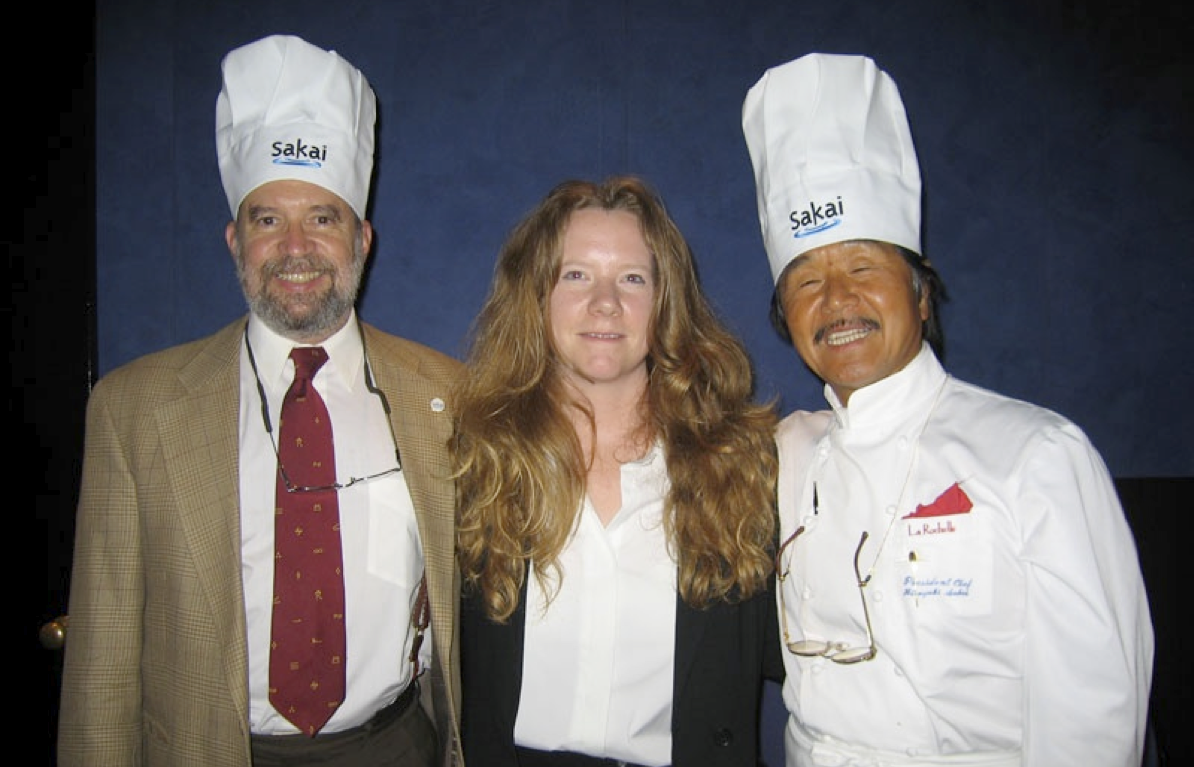
\includegraphics[width=0.7\textwidth]{images/Susan-Joseph-Hirouki-Trim.eps}
\caption*{Joseph, Susan, and Hirouki (In Tokyo)}
\label{overflow}
\end{figure}

Hiroyuki did not speak any English but it was clear that
he found it pretty humorous that a bunch of Americans had
named a software product after him.
They took a picture of Joseph, Susan, and Hiroyuki with Joseph and
Hiroyuki wearing their white Sakai chef hats.

The week of May 17 was our first integration week.  I knew that
the only way we would get all the little details of Sakai 2.0
wrapped up would be a week of co-development by the technical
leads of the project.  We just had to get into a room and
sit around the table and things would work out.  The people
at integration week included: Lance Speelmon of Indiana,
Chen Wen of Indiana, Glenn Golden of Michigan,
John Ellis of rSmart and OSPI,
David Haines of Michigan,
Gonzalo Silverio of Michigan,
Jim Eng of Michigan,
Zhen Qian of Michigan,
Beth Kirschner of Michigan,
Jon Andersen of Michigan, Daisy Flemming of Stanford, and
Josh Holzman of Berkeley.

The week went really well.  In the first two days we moved very
quickly though the issues list and by Thursday we were starting
to relax a bit.  I set up a camera to record a stop-motion
animation of our activity, added some funny music and uploaded
it to Google Video.

With John Ellis in attendance, we spent some time looking at the
kinds of issues that we would face when we would bring OSPI
into Sakai.  John was one of the technical leads of OSPI and
knew the internal details quite well.  We wanted to identify
if there was a set of small, safe changes that we could make
in Sakai 2.0 that would make it easier to bring OSPI into Sakai
2.0 over the Summer.

One of the most critical features of OSPI was that it needed
to override the default security system at times when it needed
to access files that were included in a portfolio.  As an
example, a student might upload some of their writing to
their workspace in Sakai, and then add that writing to
a portfolio presentation.  The student would then give permission
to several portfolio reviewers.  The reviewers could see
the file if they were looking at the portfolio, but they
could not see the file as originally stored in the user's
workspace.  And if the student removed the reviewer's
permission from the portfolio, the reviewer could no longer
access the files in the portfolio.  In essence, the portfolio
permissions trumped the file's permissions when the
file was being viewed through the portfolio.

We looked at how this was accomplished in the OSPI code that
was based on Sakai 1.5 and felt that it was not very elegant
and prone to failure but that we might come up with a better
idea that would fit nicely in Sakai 2.0 and have value well
beyond portfolio applications.

We broke for lunch and continued talking about the problem
while we ate.  We reduced the requirement down to its simplest
form and realized that all we needed was the ability for any
tool in Sakai to be able to request an override
of a low-level Sakai permission on a file.  The tool would
look at whatever configuration it needed and make the
ultimate decision whether the viewer had permission to view
the file.   If the tool approved the user, they would set
an indicator that would bypass all further security checks
for the file.

We called the idea a SecurityAdvisor and had it
implemented and checked in by mid afternoon.  It was an
example of just how effective the face-to-face time could be.

Lance and Chen had become our experts in bringing Java
Server Faces tools into Sakai 2.0.   They brought their own tools
into the Sakai 2.0 framework and Chen had written the
required implementations of the grade book facade code that
connected the grade book with the rest of Sakai.
With Josh Holzman with us at integration week and Ray Davis
working remotely at Berkeley, we were able to connect
Chen's work with Josh's work, all the while with Glenn
and Lance available to help at any time.

Jon Andersen and Daisy Flemming worked on Samigo all week
long and made a lot of progress.  Slowly but surely, as the
other integration problems were solved, Lance turned his
attention to Samigo which was our last remaining item that
was problematic.

I think that one of the reasons that everyone was so
focused during integration week was because of
the recent tension around inclusion of OSPI in the
Sakai 2.0 release.
They too had been through the last fifteen months of
delivering software that was less than stellar technically
and usually months late with poor quality and poor feature
sets.

We knew that this was the last major effort that we would
function as a ``core team.''   Increasingly as 2005 would draw
to a close, our approach would become more inclusive and
less well funded and our team of 15 developers would evolve
to an open source development community with committers
from many schools around the world.  I think that we all
wanted to produce a release that reflected well on what we
as the core project team had accomplished.

As integration week came to a close, we were in pretty
good shape on all fronts except for Samigo.  Samigo was
just too complex and we were trying to do too much at the
same time.

We were trying to finish the Quality Assurance on Samigo
running in Sakai 1.5.1 at the same time as we were trying
to connect Samigo to the grade book while we were
connecting both Samigo and the grade book to the new Sakai
2.0 framework. There were just too many moving parts.
With the planned code freeze only two weeks away,
it looked like once
again, Samigo would simply not make the release.   We had
released Sakai 1.5 without Samigo, and the Quality Assurance
of Sakai 1.5.1 was struggling with making Samigo work.

We knew that if Samigo did not make the release
fall production would be a disaster at Indiana.
Indiana had been apologizing to their users for the lack
of a assessment engine for nearly a year and
they promised all would be well in fall 2005.

In the weeks after Integration week, Lance spent nearly
all of his time on Samigo.  He just picked it up and made
it his problem.

We released Sakai 2.0.0 Alpha 2 on May 23, 2005.  At
this point we started Quality Assurance in earnest.
By May 26, things were looking really solid and I sent
the following message to the team:\\
\\
\begin{sf}
The problems with transactions and Hibernate Mike and I
mentioned this afternoon were resolved by about 4PM with
a quick QA and signoff by Lance, Daisy, and Jon.\\
\\
We are on track to tag Sakai Alpha3 in about an hour and
issue another internal release.\\
\\
Some cosmetic fixes to Samigo in terms of frame height
were also done so you can see Samigo in its real glory on
my nightly box.\\
\\
It looks pretty.\\
\\
Stop being nervous about 2.0 for a few minutes and feel
very proud of the team.  Then go back to feeling nervous :)\\
\end{sf}

I sent the following note to Brad, Joseph and Rob on
May 27:\\
\\
\begin{sf}
I just want to quietly let you know the magnitude
of Lance's contributions to Sakai over the past two weeks.\\
\\
While Daisy and Jon are doing a great job with Samigo
and working very hard, Lance has made extra effort
to dive into Samigo and figure out any
and every technical sticking point - within *hours*.\\
\\
Yesterday he re-factored a bunch of code (i.e.  Cleaned it
up) just so we could solve the transaction problem.  It
sounded scary to me when he proposed the idea to me at
10AM *yesterday* on the phone and now less than a day
later it is complete, tested, in CVS, tagged, released to
QA and Daisy is on her flight to Germany.\\
\\
In addition to the technical aspects of his work, he has
been sensitive to people's egos as he goes in and does
surgery on Stanford's code.  Everything he has done keeps
everyone in the loop and makes sure that Daisy buys into
and supports his work before he goes in and fixes things.
He does not expect accolades at all - he just passionately
wants this to work.\\
\\
Not to take away from anyone else's contribution over the
past two weeks - but you should be very proud.\\
\end{sf}

I had known all along that there would be countless tiny
issues and had built a few weeks of time to find and
fix the little issues with Sakai 2.0.

On May 25, I made a trip to Indiana to begin the work
of integrating the OSPI capabilities into Sakai.  I had
promised that we would start the work in earnest after
Sakai 2.0 was released and that we would take the
time to do it right.   The May 25 meeting was the kickoff
of the design work around the modifications needed to the
Sakai Resources tool (file uploading and management) to
meet the needs of OSPI.  The idea was that we would look
at all of the slick features of the OSPI replacement for the
resources tool and move them into the existing Sakai
resources tool so it would serve the needs of both OSPI
and Sakai.

On June 7, 2005, Glenn sent the following message to the
Sakai public developers list:\\
\\
\begin{sf}
I'm pleased to announce the pre-release of Sakai 2.0.0.
This is a release candidate that we are testing in
preparation for the final release June 15th. You are
welcome to download it and give it a try. I'd hold off
on going into production with it before the final release,
though :-) We will likely have one more candidate (rc3)
at the beginning of next week, before our final version
on the 15th. You can get the rc2 release from our
pre-release area (see attachment). The code in cvs is in
the "sakai2" module and tagged "sakai\verb"_"2-0-0-rc2". Simply
unzip (windows) or un-tar/gz (*nix, mac) the -demo file,
and see the readme for instructions about how to start
the included tomcat and Sakai.\\
\end{sf}

As tight as the 2.0 development cycle was, we did not have
a lot of time to run Quality Assurance on the release.
Most of the Sakai code was taken straight from Sakai 1.5
which had been given a lot of QA attention.  The grade book
was relatively simple and had a lot of testing as part of its
development at Berkeley and MIT.   Samigo had been
passing the Stanford QA tests
all along in terms of functionality.  And as we began testing
the early releases in mid-March, everything felt solid
to me so it did not feel like we would need to slip
the planned June 15 ship date to allow for more Quality
Assurance.

The only risk in the back of my mind was Samigo.  I was glad
it was finally solidly in the release, but since it was
large and complex, I was a bit worried.  Developer testing is
great but it always misses something and it is particularly bad
at catching problems that happen when software is run in
production at high usage levels.  In my experience, at some point
the only way to catch the remaining few things is to go
into production, encounter the problems, and then fix them.
While we could have slipped the schedule to allow more
testing time, my feeling was that it would barely improve the
quality of Samigo.  With all of the pain that we had endured
to make the schedule, a schedule slip for more testing
that I was pretty sure would not really improve the quality
very much seemed like a bad idea.

\chapter{Lost in Transition}

While the Sakai technical team had been building the release
for the world, Joseph Hardin and the Board had been preparing
for the end of the grant and transition to the project becoming
a stand-alone 501c3 non-profit corporation.   At this point,
with over 100 members and a million dollars of annual revenue,
we needed a business structure rather than a grant account
at the University of Michigan.  Most grants have a fixed
time period and then they are completed.

Sakai was going to have revenue and expenses for years to
come and universities get a little nervous when faculty
operate businesses from within the university.  The
university properly insists that all expenses follow university
policy and if Sakai were to hire staff, they would be hired
as University of Michigan employees, and if there was a contract
to be negotiated, the university would need to get involved.
For those and many other endless details, it was important
that we shift the revenue and expenses from the University
to a non-profit organization.

Joseph had spent a great deal of time researching the formation
of a corporation, building a set of draft bylaws for the
organization, and working with the Board and community with
those bylaws to build consensus around our future governance.

I had not been particularly involved in the formation and
discussion of the bylaws because building Sakai 2.0 had taken every
ounce of my energy just to get it completed.  And I trusted
Joseph to get the bylaws right.  I really had little patience
for long consensus building discussions when I felt the
answer was obvious, but it was going to take
another hour to ``socialize'' the answer.  These
discussions were quite important, they were simply not
something that I enjoyed.  And since I was overbooked time-wise
it was just as easy to miss those meetings.

With Sakai 2.0 looking like it would be successful, I was
starting to spend more time ``promoting our brand'' than
managing a technical team.   I had been working with Scott
Morris of Apple for about a year discussing
whether or not there was a place for Sakai in an Apple product.
Apple has a strategy of bundling free open source software
as part of their OS/X Server product.  I think that Apple's
idea was to cede the raw, basic UNIX server market to Dell and Linux
and make it so that OS/X Server would pre-include all of
the useful software and have a nice simple management
interface.

Our ideal use case was that a small school would want Sakai
so they would buy an Apple X/Serve, install it, press a few
buttons in the user interface and voila!  They would have a
Learning Management System.   All the upgrades and security
fixes would be distributed along with all of the OS/X Server
fixes.

Scott and I did a lot of talking and eating Sushi in Mountain
View, but with Sakai in a constant state of change, we never
really had a moment where the Sakai software was stable enough
to suit the requirements of the X/Server team.  They really
wanted a mature package that would just put out a few patches
here and there.  They did not want major conversions of
user data to happen as part of an X/Server upgrade.

But Scott and I felt that some point in the future, we
might still be able to make it happen.  And in general, we
wanted Apple to have something to talk about in the teaching
and learning space so Scott got me several speaking engagements
in Apple venues.

My first presentation was to the Apple developers at the Apple
Worldwide Developer Conference on June 15, 16 in San Francisco,
CA.  Giving a talk at an Apple Conference is a lot of fun.
I had to prepare my slides well in advance and provided them
to Scott, who gave them to Apple marketing and an Apple graphic designer.  Then
we would go through a series of reviews of the slides.  They
worked through the content, asking me to simplify slides and
move toward a more ``Steve Jobs'' style of presentation where
we would communicate ideas using simple pictures, words, and
graphics on the slide rather than long sequences of text
like I used when I was teaching.  The graphic artist redrew
all the diagrams, simplifying where necessary and adding lots of
pretty eye candy.  The backgrounds of the slides were all black
and the text was all white or bright colors (like Steve's slides).

They made me give the presentation several times to different
small groups from Apple Marketing.  Their comments focused mostly
on me simplifying my narrative and hitting the high points.
I mostly think that they just wanted me to practice before
I got up in front of the crowd at their conference.  They were
sensitive to the fact that when they put me up in front
of their crowd, I was part of their brand.  As a dedicated Apple
fan, I was more than happy to fit into their marketing and
reinforce their messages as much as possible.  After all,
I very badly wanted our Sakai software to fit into their OS/X
Server product.

The presentation went well.  I was disappointed that the audience
was a bit small, but was pleased that I had spoken at an
Apple Developer's conference.  After my talk, I attended
a number of other sessions including how to build an
automatic installation package for Macintosh OS/X.  Sitting
in the back of the session, I built an install package that
allowed you to install Sakai 2.0.0 on a Mac OS/X system in a few clicks.

The Steve Jobs keynote is the highlight of each Apple World Wide Developer Conference
(WWDC).  Of course he is a great speaker
and he loves to introduce new things at the annual developer's
conference.  Since it was the last few days before the Sakai 2.0
release, I spent most of Steve's keynote on my laptop
working on Sakai using the wireless network.

Then Steve announced that the next generation of Apple computers
would support Intel processors and that their support
of the PowerPC would slowly be phased out.  A chill of excitement
went up and down my spine as I immediately realized how brilliant
this would be.  It would allow dual booting of Windows
and really great Windows emulation on the Macintosh.  And
since Apple OS/X was UNIX it could easily be ported from one
hardware architecture
to another while Windows was stuck with the Intel
architecture.  At the same time, the Intel architecture was
cheaper, used less power, and ran faster except for a few
floating-point calculation operations where the PowerPC
had an advantage.

Next, Steve told us that he had a secret lab with five employees
that had kept all of the versions of OS/X running on Intel
hardware for the past four years --- since Mac OS/X 10.0.
I loved this approach where he always kept a ``Plan I''
ready in case the PowerPC processors were
(a) too expensive, (b) used too much battery power, (c)
ran too hot, or (d) could not improve performance rapidly
enough.  When all these became true, it was time to switch
to Intel.

Then Steve talked about an emulation mode called ``Rosetta''
that made it so that old PowerPC software could run on the
new hardware with virtually no performance impact.
He showed us that the computer he had been using all
along to do his presentation and all of his demonstrations
was an Intel processor running most of the software in
emulation mode.  My jaw dropped to the floor.  Steve said
that as we would walk out of his talk, there were several
rooms that would be opened where we could play with working
hardware prototypes and test our software on the newest
version of the Apple operating system running on Intel
hardware.

I ran out and quickly tested Sakai on the new hardware.
It was more than twice as fast to compile and start Sakai
on the new Intel hardware when compared to the older
PowerPC hardware.
The time to start Sakai was 81 seconds on a PowerPC Laptop
and 31 seconds on the new Intel-based prototype Apple
hardware.  I wanted one of the Intel-based Apple systems
just for my own development productivity.
I walked out of the session and called my brother-in-law
and in passing, told him that I believed Apple stock would
triple in three years.
I told him that it would only be a matter of time
before Windows would work wonderfully on the new hardware
and having both Windows and Apple on the same laptop would
be a powerful new way to work with computers.  He took my
advice and invested some of his spare cash in Apple and
did very well the next few years.\footnote{On June 13, 2005 
Apple stock was trading at
38.31 and on June 9, 2008 Apple stock was trading at 172.37.}

For me, it was a exciting feeling.  Our Sakai product
was emerging at just the right time and if we played our cards
right, we might even be able to be included in some
future version of the Apple server operating system and through
that we had the potential of literally thousands of smaller
schools that would be able to run and manage our software
with just a few clicks.   Sakai was going to be a rising star
and I was going to make it happen.

I was really looking forward
to the Sakai Partners meeting the next week
in Baltimore June 8-10, 2005.  It would be the first meeting
where I was not apologizing for a schedule slip or missing
functionality.  It would be the first meeting where I was not
going to have to explain how I got it wrong in the grant
project plan and had come up with a new plan.

Our software was (mostly) elegant, it was (mostly)
production-hardened, it finally had a grade book and
an assessment engine, it supported multiple languages,
its architecture and developer patterns were clean and reasonably
well documented, it had Web Services, and it was coming
out for release the following Wednesday and you could
play with it \emph{right now}.  I kind of felt a bit like
Steve Jobs.  It would be nice to surprise and delight
our Sakai Partners for once.

This was a stark difference when compared to the previous
conferences where I believed there was a decent chance of being
lynched by our partners at each one.  The number of attendees
at the Baltimore conference greatly exceeded our estimates.
People were coming not just to
monitor our progress, but to begin to plan to adopt our
software.   It felt more like a user and adopter conference
than a developer meeting making reports to our partners.
The small rooms were all overflowing
and the presenters were having a great time.  We had to
re-do several of the presentations more than once because there
was so much demand.

We had increased the number of tracks, and provided tracks
for end-users, portfolio, and quality assurance, along with the
traditional developer tracks.  These new tracks reflected
our transition from a heads-down grant-funded group building
software to being a much larger community of interest around
our emerging product that we would soon collectively own.

It was particularly satisfying to see all the members of the
Sakai team getting attention and accolades for the work they
had done over the past 18 months.  And the OSPI / Sakai 2.0
tension of the past few months seemed behind
us.

Baltimore was also the first time we allowed people to attend
from schools that were not yet partners.  Up to that point,
you could only come to the conference if you were a partner,
and if you were a partner the conference was free.  The food,
drink, snacks, and wireless Internet were all paid from the
member dues.  And we hosted some pretty fun conferences.

For me, this was the first conference where I was no longer the
center of attention.  I had a few talks on architecture and status
reports, but increasingly those were just one of many talks.  I
liked the new pattern.  I spent a lot of time in the
hallways and in small rooms with the technical team, going over
the final testing and details around next week's release.

Our keynote speaker was Brian Behlendorf of the Apache
Foundation.  His speech was perfectly timed as we were imagining
how our community could become a Foundation like his Apache Foundation.
Brian eloquently described all of the open source principles
that I so passionately believed in.  It felt great to have his
commentary on the very day before we were going to have a
whole day meeting discussing and editing the by-laws for the
soon-to-be-formed Sakai Foundation.

I was more than happy to be too busy to sit through the bylaws
discussion.   Joseph had recruited John Norman of Cambridge and
Chuck Powell of Yale to lead the bylaws discussion.   He wanted
to make sure that the bylaws reflected the entire Sakai Community
and not just the Sakai Project institutions.  This made a lot
of sense because going forward there would be no ``core schools''
and ``Sakai Partners.''  Everyone would simply be members of the
Sakai Foundation working together.

The bylaws conversation went well, each time I read
a draft, I was always pleased.   Everyone was doing a great
job looking at Jasig, Apache and other foundations that had
come before us and making wise choices.

Sakai 2.0.0 shipped Wednesday June 15, 2005.  The feature list
for 2.0 was:
(a) tools user interfaces reworked to be style guide compliant,
(b) new portal navigation (Charon),
(c) improved ability to customize the user interface (re-skin),
(d) re-written framework,
(e) supported any number of languages,
(f) grade book,
(g) assessment engine,
(h) web services support,
(i) architecture design documents, and
(j) improved install documentation.
It was an impressive feat for a hard-working and talented
team of individuals.  The timing was perfect for us to take
our place in the market.  We had opened a window into the market
in January 2004 and had driven through that window in June 2005.

There was no time to celebrate. I had sold my soul to keep
OSPI out of the Sakai 2.0 release and I had promised I would
make it good with Indiana over the summer.  Indiana was going
to put a lot of energy into bringing OSPI into Sakai 2.0 so
they could run it in production in the fall. I would be spending
a lot of time in Indianapolis and Bloomington over the summer.
Our first meeting to work on moving OSPI into Sakai was a
week after the Sakai conference on June 17.

We also had another fun trip on June 20-22 to the 2005 IMS
Alt-I-Lab conference in Sheffield, England.  It was time to
demonstrate the implementations of the IMS Tools Interoperability
specification.  Travel to a fun location, having drinks and
dinner together always rebuilt team cohesion.  We could talk
tension out and forgive each other and talk about the future
instead of the past. And if I had offended anyone on the team,
I could apologize over beers.

In particular at this meeting, it was a bit of an
introduction of Sakai to the marketplace with most
of the international players in the LMS marketplace present
at Alt-I-Lab.  Unlike at the Sakai meetings, Sakai played
a relatively small part.   There were no keynote speeches about
Sakai.  At this meeting, Sakai was a product in the marketplace.  And most
importantly, if you look at who had shown up, it looked like
the market leadership was Blackboard, WebCT, Moodle, and
Sakai.  ``And Sakai'' sounded so wonderful in particular because
I knew that our 2.0 software was very strong.  Thanks to the
work of Beth Kirschner and the team at the University of Lleida,
we were truly ready to play on the international stage.

The real work of the demonstration fell to Anthony Whyte
of Michigan and Lydia Li of Stanford.   There were only two
tools that had been part of the demonstration along with the
four learning management systems.  But Samigo was the only
real assessment engine.  Assessment was the core use case
of the Tools Interoperability approach.  Tools Interoperability
could launch a tool and have a score sent from the tool back
to the LMS.

Samigo was the star attraction.  All of the LMSs
did their demonstrations focusing mostly on how
Samigo worked in WebCT, Blackboard, Sakai, and Moodle.
During the run through the day before the demo, we stressed the
hotel's network and Internet infrastructure so badly that they
had to drive up from London with new network hardware.  But for
an experienced demonstrator, this was just par for the course.
If you look at my video from Alt-I-Lab 2005, you can see Anthony
and Lydia relaxing after the run-through, totally confident
and relaxed.

Anthony Whyte had picked up the development tasks around the Sakai
implementation of Tools Interoperability since I had so much
going on with Sakai 2.0.  I pretty much was a cheerleader for
most of the Tools Interoperability work while Lydia and Anthony
did the hard work.

The demonstration went well and the crowd was pleased
to see the four competing LMS systems cooperating. It showed
a window towards a possible future where standards would
increasingly make it less important which LMS you had.  There
was a long way to go, but it was time for celebration.

The Tools Interoperability group celebrated both
at Kevin Riley's house and a pub in Kevin's
neighborhood.   While we had been meeting and working with Kevin
all around the world as the project manager for the IMS Tools
Interoperability specification, Sheffield was Kevin's hometown.  So
the whole IMS Tools Interoperability demonstration group
trouped over to get a tour of Kevin's amazing bachelor pad.
After the tour, we went to the Kelham Island Tavern
down the hill from his house
and celebrated with some food and a few beers.  I love small,
local, unique, intimate dining experiences and this was perfect.
Kevin even knew the dog that lived in the pub and the dog sat under
the tables as people talked about everything under the sun.

The next day, it was time for the IMS Technical
Advisory Board meeting and introduce the idea of the
IMS Common Cartridge that we had discussed with the publishers
back in April at the Stanford meeting.  Ray Henderson
of Pearson Education introduced the idea of developing a standard (IMS CC) 
to be a common import and
export format for publishers and learning management systems.
The timing was perfect and we had the perfect person doing the
presentation.  We had just finished a great demonstration
of how all the marketplace could work together cooperating
instead of fighting.  The IMS Common Cartridge idea
went over unanimously and in the excitement, we promised
that we would have an equally awesome demonstration at
the Alt-I-Lab 2006 conference that would be held
in Indianapolis, Indiana.

For me the week at IMS Alt-I-Lab in Sheffield reminded me that
my goal for Sakai was to change the marketplace.  It
was clear to me that we *could* use the influence of Sakai
as a gentle agent of change in the marketplace.  As we had built
the IMS
Tools Interoperability specification, the University of Wisconsin did the
majority of the
Moodle work without help from the central Moodle development
team.
Blackboard participated in the specification development
and demonstration but they were never leading the design work.
Since WebCT and Sakai had jumped headfirst into
Tools Interoperability, Moodle and Blackboard had to
come along for the ride or they would have been left out.

Since Sakai and WebCT were the up-and-coming LMS systems
and Blackboard was the entrenched old-guard in the marketplace,
Blackboard knew that if the cowboys (Sakai and WebCT) were
successful and Blackboard was shown to be a ``foot-dragger'', that
both the smaller players (Sakai and WebCT) could use it
against Blackboard in their marketing.

I liked working with Chris Vento and the others from
WebCT.  They liked new ideas and were a more
agile company than Blackboard and were far more willing to
take risks and invest in emergent
ideas.  I knew that I could build up the alliance between WebCT
and Sakai and use it to gently begin to move Blackboard in the
right directions.

The next week, on my way back from England, I stopped in
Washington, DC and with Jim Farmer's help I had my first
face-to-face meeting with Martin Dougiamas, the creator and
lead on the Moodle project.  Martin is a great guy with
great charisma and we hit it off right away.  I felt
absolutely no need to compete with him.  We talked for a while
and I shot a short video interview so I could introduce
Martin to the Sakai community to make him seem less
of an opponent and more like a fellow innovator working on the same
challenges as we were.   Moodle and Sakai were more like cousins
than enemies.

On July 4 2005, John Merlin Williams, the Executive
Director at the University of Michigan Media Union, asked me how
I was doing and I replied with the following message:\\
\\
\begin{sf}
Keeping one step ahead of things.  The big conflict is and
will likely continue to be the "inside of Sakai" politics
versus the "outside of Sakai relationships and opportunities".\\
\\
These two pools of thinking need to inform one another,
but the "insiders" are all focused on the next three
months building a learning management system.\\
\\
People like Joseph, Brad, and Rob Lowden also operate in
both arenas so it is not so bad, but hopefully after the
first of the year the "Sakai insider club" will be a
little less self-focused.\\
\\
Until then it seems like I lead a split life :)\\
\end{sf}

On July 18, 2005, we had our first community developers meeting
at Yale University.  Now that we had delivered Sakai 2.0,
it was time for me to focus on enabling more schools
outside of the core to adopt and install the product.  Our
documentation was weak so we hoped to just get people
from the community together and work through the issues.

As the workshop started, I gave a few presentations
that covered Sakai at a high level and when I finished,
I opened the floor for questions.  The questions quickly
moved into areas that were beyond my expertise. In reality,
I was one of the less technically skilled people at the
workshop and there were clearly a lot of details about
Sakai that I was unaware of.

But before it became clear that I was clueless,
the workshop attendees started answering each other's
questions.   While I had been distracted trying to manage
the project, others in the community were digging through Sakai
to figure out how to install it and make it work.

It got so bad, that at one point someone asked if we could
have a tool that would allow technical support staff to
switch into a user's account so they could check to see
if the user was having a problem.   I gave a long answer
that talked about how hard such a tool would be to build
and what parts of the Sakai architecture would need to be
addressed to build such a tool.

When I finished my little speech, Zach Thomas of Texas
State San Marcos piped up from the back of the room and
said, "I already have written a tool to do what
you need and you can download it and use it.".

As the day went on, I increasingly realized that the
Sakai community was already quite strong and that
I no longer needed to be the only
expert on all things Sakai.   Since we were open
source and we had a lot of schools interested in Sakai,
we had a lot of bright people in the community that
were starting to take care of each other.

It was a great feeling to know that as we were
finishing the grant-funded phase of the project,
we already had a growing talented community that
would own the project starting in 2006.

At the end of the first day, I sent the following
message:\\
\\
\begin{sf}
The Yale meeting is going really well.  We have a
number of short presentations.  \\
\\
We have covered a lot of ground:\\
\\
-  Andrew Poland's talk about how IU runs in Production\\
-  Seth Theriault's discussion of perl and web services to
   pre-populate courses in Sakai 2.0\\
-  John Leasia redid his Baltimore talk.\\
-  We had an overview of CAS from Yale\\
-  We had  talk about Shibboleth from Steve Carmody
   from Brown\\
-  Zhen talked about providers\\
-  Jon Anderson talked about how UM maintains our
   production environment\\
-  Vihsal from SunGard is here and we are doing some
   initial WSRP integration for 2.1\\
\\
The breaks are buzzing - lot of code being worked on and
people sharing stuff.\\
\\
Walking away from this meeting I am far more comfortable
that our fall 2005 sites will actually make it.\\
\end{sf}

As the meeting wound down on the second day, and
I was starting to relax,
several attendees started a conversation
about their complaints
about the QA in Sakai 2.0 and complaints as to how
priorities were set in the project.
The points everyone brought up were
reasonable and mostly due to the difference between
the priorities that the founding Sakai organizations
needed to pursue for their own production needs and
to meet the requirements of the initial Mellon grant
which was to be completed December 2005.

I had no good answers to the complaints.  So I just
let them vent.  For me it was frustrating to end the
otherwise successful Yale developers meeting with
negative energy.

As we moved from July into August, the Indiana and Michigan teams
were installing, configuring, and testing their
Sakai 2.0 production environments.   Since I was
not directly involved in either school's production
environment, this gave me a good chance to work on
my National Science Foundation grant tasks, so
I scheduled a weeklong trip to Indiana and Illinois
the week of August 8-12.

The week started very well. Over the weekend before
I left for Indiana, I had built a JSR-168 portlet that allowed
us to plug a simple version of the Sakai user interface into
any of a number of JSR-168 compliant portal systems.  It felt
good to be making progress on both the research and teaching
and learning applications of Sakai.

But on Thursday August 11, I found out that Indiana was having
significant problems with Sakai in production.  It was running
out of memory and then hanging and crashing.  Michigan was not
crashing under similar testing and load.

Unfortunately, I was not experienced in the subtleties of
running a complex Java application like Sakai.  The
University of Michigan was not yet running the Samigo testing
engine.  Indiana needed to run Samigo because the system they
were replacing had a testing engine.

Because Indiana and Michigan were running different
configurations, it did not look like the Michigan team would
be able to help Indiana.  And I did not have the skill to
solve their problem.  The only other school that might be
able to help was Rutgers University.  They were also going
into production with the Samigo testing engine.

On the morning of August 12 at 9:41AM, I sent this note to
Chuck Hedrick and Bill Crosbie at Rutgers.  Chuck was
the Chief Technology Officer of Rutgers and Bill was a
developer on the Rutgers Sakai team.  Both were active Sakai
developers.\\
\\
\begin{sf}
Bill and Charles,\\
\\
Indiana is struggling with a memory leak (we
are guessing that your memory leak is the same
problem).  I suggest that we work together and
share knowledge and results.   Our basic problem
is that neither IU nor UM have much experience
with memory leaks.  Neither IU nor UM has much
experience with profiling.\\
\\
Here is a summary of the situation:\\
\\
- IU is running some code beyond 2.0 and
using Samigo/Grade Book (GB) and running out of memory\\
\\
- Rutgers is running stock 2.0 and Samigo/GB
and running out of memory\\
\\
- UM is running code beyond 2.0 (mostly 2.0.1
plus local stuff) without Samigo and *not*
running out of memory.  UM is doing heavy testing
of the application with stress tests, and has
seen no memory related problems.\\
\\
We suspect the Samigo or GB code mostly because
those are new and to date has not run in large
production like much of the rest of the software
but have no real evidence at all of that
hypothesis other than the information above.\\
\\
Bill and Chuck,  I would be most appreciative if
you could contact Andrew Poland quickly and
share knowledge and help if at all possible.\\
\\
Anyone who has something to add should feel free
to comment on this to this group.\\
\\
Thanks in advance.\\
\end{sf}

I sent the note just hoping against hope that something
good would happen because I knew that I would not
be able to figure out their problems.

By noon, Bill Crosbie had responded with an initial
assessment of the problems and a summary of what
Rutgers was doing and had been doing.
The message was very detailed with
a clear roadmap of what was wrong and what steps
Rutgers had taken in investigating the problem
and what steps Indiana should take to further
investigate the problem.  The following is just a
small part of Bill Crosbie's message that went on
for several pages.\\
\\
\begin{sf}
On Aug 12, 2005, at 11:59 AM, Bill Crosbie wrote:\\
\\
I think Chuck [Hedrick] is in meetings for the day,
so I am taking first responder role.  C. Hedrick will
surely respond with more detail on top of this.\\
\\
When we were getting OoM [Out of Memory] errors we
noted that there was plenty of physical memory still
available, but it was not being used.  There was a
lot of suggestions about config parameters, but there
was little understanding of what was actually
happening in memory.\\
\end{sf}

With Rutgers coming to the rescue, I could again breathe
a sign of relief.  We had made it past another
crisis that had the potential
to derail the project, and as was to become an increasing
trend we found the talent to move the project forward
from sources outside the four founding universities.

On August 16, we released the Sakai 2.0.1 release
with over 160 bug fixes and improvements.  This was
timed so schools could upgrade in time for the start
of the fall semester.

Two days later, we had another Sakai Developer's meeting
at the University of Michigan in Ann Arbor.  It was a
lot of fun and a good time for us all to spend
time together and plan for the upcoming semester.

One of the attendees at the Ann Arbor meeting
was Steve Githens.  He was a
programmer who just loved being part of an open
source project.  He had recently graduated
from Michigan Technological University and was working
as a Chemistry lab assistant at Northwestern University.
Without ever meeting anyone in the community or working
at a Sakai school,
Steve had built and distributed a set of simple
web service end-points that many schools
were already using to
handle repetitive or automated administration tasks
for their production Sakai systems.

I made a video where I interviewed Steve and asked him
about his ideas regarding what it was like to
participate in Sakai and some of the ideas and plans
he had for Sakai.   You could easily see his excitement
and the energy he brought to his work in Sakai.

In September, as part of the ramp-down of the
grant phase of the project, we disbanded the "Tools
Team".  The Tools Team and Architecture Team were the
two planning structures that guided the grant phase of the
project.   The Architecture team was more of the
technical members of the project while the Tools
team focused on the user features and style guide
for Sakai.

There was some natural tension between the desires
and goals of the two teams.  For me, the problem
was that we never were out of a crisis for long
enough to allocate resources to most of the issues
raised by the Tools Team.  This led to the Tools
Team feeling that they were generally ignored most
of the time.

% http://bugs.sakaiproject.org/confluence/display/REQ/2005/09/09/Sakai+Core+Requirements+Process

The Tools Team wrote a final report that summarized their
activities and views of the project and put it in
our Sakai wiki.  A few excerpts from that document
capture the sense of tension and disappointment.\\
\\
\begin{sf}
\\
"The Architecture Team, like the Tools Team,
had representation from each of the core schools. The
Team met regularly to build consensus, but almost all
framework-related decisions about what did and didn't
get done ultimately were made by the project lead and the
framework architect. Again, it is not clear to what
degree functional requirements were considered in the
deliberations and making decisions."\\
\\
"Having been the lead on most of these
requirements gathering efforts, I think I can safely say
that they have been largely ignored in subsequent
development activities, the one exception being Course
Management (in development now)."\\
\end{sf}

It would be fun sometime to go back in time and do a project like
Sakai without any time pressure and whenever something
went wrong, simply slide the schedule out a bit to allow
sufficient reflection and time to recover.  Unfortunately
if you have the luxury of slipping schedule in an attempt
to make everyone happy, you usually end up with a product
that never ships.

Reading the report felt like a personal failure on my part
to do more and be more responsive to their issues.  But
at least we had shipped software and that software was
running in production at scale at two schools.

In a sense, given that we had started on the Sakai
2.0 rewrite in January 2005 and were in large-scale
production at two schools in September 2005, was a
testament to our ability to ``make an omelet'' even
if we had to break few eggs in the process.

Now that we had software worth keeping for the long run,
it was time to build a strong worldwide community to sustain
Sakai.

\chapter{The Great Beyond}

As September 2005 started, it looked like Sakai
was here to stay.   With Indiana and Michigan
solidly in production and a number of other
partner schools putting it into production, it looked like
there was more than enough commitment to the
Sakai software to insure that we would have a solid
long-term open source project with a diverse and
supportive worldwide community.

I had a busy fall planned with lots of travel, so before
it all started, I took Brent up to Leota, Michigan
for a weekend of dirt bike and ATV riding in the
pinewoods of Northern Michigan.  Over the
summer he had become an accomplished rider and he
was quite good at ripping around the high-banked
sandy corners on the trails through the woods.

We were starting to drive fast enough for it to
be fun for me and each time we would take a ride
he would push himself even further.  I took lots
of pictures and videos of his ever improving
riding ability.

We stayed at a small hotel called the Leota
Lodge and eat all of our meals at the Riverside
Bar (the only restaurant\slash bar in town).  We had been
to the Riverside Bar enough times that the staff
greeted us by name and knew our orders.  Given that
Brent always arrived in hand-crutches, it never
took anyone too long to remember us.  It was a lot
of fun to get away from the meetings and airports
and just hang out with Brent in the woods.

On Sunday, we got up and took a few rides before
packing up to go home.  It had been a great weekend
and we kept going faster and faster as confidence
grew.  By the third ride of the day, we were
starting to get a little competitive.  As we came
around one corner onto a straightaway at about 20
miles per hour, Brent's ATV drifted to the side
and his left front tire caught a root that stuck
out of the side of the trail and he rolled his ATV
right in front of me and he ended up underneath
the ATV.
In a moment, I was off my motorcycle and at his
side.  His 90CC ATV was quite light and I easily
lifted it off of him and set it upright.  Luckily,
he had landed in soft sand and the ATV was so
light that he was not hurt at all.
I picked him up out of the sand and sat him
on the side of the trail and brushed him off.

We sat for a bit and then laughed as we
decided that perhaps we had reached the limit
of how fast we should be going.  We decided
that from that point forward, our goal would no
longer to be to go faster and faster but instead
to slow down a bit and have more fun.  And in
particular, we would stop racing with each other
to see who was the fastest rider.

After a bit, we hopped back on and finished
the ride back to the parking area, loaded
up the bikes and went home to get some clean
clothes and take a nice shower.

By this point my wife Teresa had decided that
all this motorcycle and ATV riding was too much
fun and she insisted that we needed to buy
her an ATV as well so she could come up and
ride her own.  So I started looking for a used
Polaris 200 ATV that we could buy for her.

Back in civilization, the University of Michigan
was running the entire campus on Sakai in the first
few weeks of September, so Joseph and I could
increasingly look towards the post-grant phase
of the Sakai community.

We wanted to get a second round of funding
with a more narrow focus of dedicating resources to further
strengthening the core architecture of Sakai.   In our
hurried Sakai 2.0 re-write in January 2005, we had run out
of time to rewrite everything so at some point we
stopped rewriting Sakai 2.0 and plugged
the rest of Sakai 1.0 into Sakai 2.0.

We felt that as the more schools adopted Sakai, there
would be increasing pressure to add user-facing features.
We felt that the open source community priorities would
not address core long-term internal architecture issues.

We wanted grant funding so we could have a dedicated
team to focus on completing the rewrite and set Sakai
up with an elegant internal
structure that would make it possible to build a number of
whole new kind of distributed teaching and learning tools.

Through 2004 and 2005, the University of Michigan had been
particularly generous making about five developers available
to me to work on the issues that I saw as high priority
for the Sakai community.  Since Sakai was based on CHEF,
my feeling was that all the requests from outside Michigan
had higher priority than the end-user requests from
within the University of Michigan.

That meant that the University of Michigan end-users of
CHEF and then Sakai saw a series of changes to the software
that were driven by community needs and desires while
their needs and desires were being put on hold.
I was concerned that the University of Michigan would
rightly want to change this arrangement once the grant
ended in December 2005 and switch their resources
from community priorities as determined by me and to local
priorities responding to the on-campus end-users.

I felt that getting a second grant was the only way to assure
that at least some of those resources would continue
to be available to work on community priorities first.
The other Sakai schools were applying for Mellon
funding for their own community source projects.
Indiana was starting their Kuali project for
open source administrative computing and Berkeley
and the University of Toronto were planning
the Fluid project.

It made good sense that the core schools that worked
on Sakai had proven their talent in the open source
space and were good candidates for the next round of
funding.   But for me as these schools moved on to
their next projects, I wanted to make sure that
Michigan received some compensation to provide
continuity for the Sakai software.

Joseph and I went to Princeton to pitch the
idea of funding architecture improvements to Sakai to Ira
Fuchs of the Mellon Foundation.   Ira had given Joseph
the original grant for Sakai and we felt that we had
done a pretty good job of delivering on the original
multi-institutional Sakai grant.   We hoped that Mellon
would see that we were a good bet for a smaller and
more focused  investment.   Ira listened to our proposal
and suggested that we write up a pre-proposal document to
get things started.  We needed to finish the Sakai project,
and put in the report before we would be seriously considered
for follow-on funding.  That made good sense to me.

We also visited Chuck Hedrick, Bill Crosbie, and
the Rutgers team on the trip.  For me it was a great
opportunity to convey my thanks in person for their help
with the performance issues that Indiana had faced
early in August.  I tried to make it clear that
without their help, we would have been in a very
dire situation.

% 2005-09-12-18 Japan Visit Sakai - Chuck and Beth

When we got back from the Princeton and Rutgers visit,
I was off on a visit to Japan to meet with the
Sakai community in Japan with Beth Kirschner.

From the moment the University of Lleida in Spain
did the first translation of Sakai, Beth Kirschner had
become the czar of Sakai translations.  She worked with
communities around the world building their translations
and getting the translations committed into the
source tree for each release.  It was an amazing amount
of technical work and more importantly it required
the right kind of person to gently motivate all
of our worldwide collaborators.  And Beth has always
done an outstanding job.

Our primary contact in Japan for the trip was
Shoji Kajita of Nagoya University.   I first met Shoji
when he was leading the internationalization and
translation activities for the uPortal project.  Shoji
was involved in his campus portal, educational technology,
multimedia, and even high performance computing. As soon
as Sakai was formed, Shoji became involved in Sakai.
He was very good at getting research grants in Japan
to work collaboratively on projects like Sakai with his
students.

Shoji had arranged the following schedule for us
in Japan:\\
\\
\begin{sf}
Sept 12: Arrive at Nagoya Airport from DTW at the evening\\
Sept 13: Aichi Expo for adjusting the jet-lag\\
Sept 14: Localization and Internationalization discussions at Nagoya University\\
Sept 15: Sakai Workshop (whole day) at Nagoya University\\
Sept 16: Hosei University in Tokyo\\
Sept 17: Sightseeing in Tokyo area\\
Sept 18: Leave for DTW from Tokyo-Narita Airport\\
\end{sf}

On the first day, to keep us moving and walking
so we would adjust to the time zone change,
Shoji took us to the Expo 2005 Worlds Fair.
We rode the Linimo magnetic levitation train
out to the Expo and had a great day.

On the second day, we met with Shoji's development
team at Nagoya University to talk about
moving beyond the problem of
simple translations of the user interface and we started
to identify needed changes to how the software
needed to function to be truly translatable.

Beth and I gave a day of presentations at the
Sakai Developers Workshop, then we went to
Tokyo for a series of meetings with Kazou Yana
and others at Hosei University.

When we got back from Japan, I took a quick weekend
run up to Leota to go ATV riding with Brent and
then it was back to the airport to begin the trip
to England and the Cambridge Sakai Developers
meeting.

One of my secondary goals of the trip to England was to make a
visit to the Open University in Milton Keynes, UK and
try to convince the Open University to join the Sakai
community.

I had been aware of the Open University since the late
1990's.  The Open University was one of the world's
leading distance-education Universities.  They had a
large campus in Milton Keynes with a large faculty
and staff but no students.
All of the education was done at a distance using
a wide range of technologies.

The Open University
was designed from its founding in 1969 to be
the ``University of the Air.''  The Open University
also had a partnership with the British Broadcasting
Corporation (BBC) and for a time, Open University
lectures were broadcast all over the UK on the
BBC channels late at night.

I found their approach and attention
to detail very impressive.
I felt that if we could get the Open University
involved in Sakai, that they would bring a lot
of creativity, talent, resources, and credibility
to our community.

Earlier, I sent a note to Martin Weller to see if I could
spend a day at the Open University.\\
\\
\begin{sf}
Martin,\\
\\
I will be in the UK with some spare time.  I added
two days in case I could spend a day at Open U.
Milton Keynes is "close" to either Nottingham or
Cambridge so it should be pretty convenient.\\
\\
Arrive Monday September 19 - London\\
Monday (19) - Thursday (22) - Nottingham for the JISC all hands meeting\\
Friday (23) - Free day\\
Monday (26) / Tuesday (27) - Cambridge - Sakai Developers\\
Wednesday (28) - Free day\\
Thursday (29) - Depart from London\\
\\
On Sep 2, 2005, at 5:31 AM, M.J.Weller wrote:\\
\\
Hi Charles\\
\\
We'd be happy for you to visit --- the 28th looks the
best bet so far. I have contacted a few others who
would be interested in meeting you. Joel Greenberg
is probably the most significant of these, but he's
on leave till Monday, so I'll come back after that
with some definite plans. But let's say the 28th
now, we'll sort out the details later.\\
\end{sf}

Once we had set up the date for the visit, we agreed that
I would give a talk about Sakai at the Open University.
It seemed like a great opportunity to bring one of the
world's leading universities into the Sakai community.

The trip to the UK started at the eScience meeting at
Nottingham, UK.  This meeting was a great time because Sakai
was different from the other learning management systems
in that it could easily be used for general-purpose
small group collaboration.  Much of my National
Science Foundation grant activity was working with
Sakai to increase its suitability for research groups
to use Sakai for their collaboration interaction.

The Nottingham meeting was the annual meeting of the
eResearch projects funded by the UK JISC
research funding agency.  Everyone showed up and made
presentations and demonstrations of their latest results.
Sakai had made significant inroads into the eResearch
community.  Folks like Rob Allan from Daresbury Laboratory
and Rob Crouchley, Adrian Fish, Miguel Gonzalez Losa,
Ties van Ark
and others from Lancaster University were increasingly
using Sakai in their eResearch projects so the meeting
was a great opportunity for me to see the work they had
done and plan our next moves.

While I was in Nottingham, I had found a Red Polaris 200
ATV on eBay so I put in a bid.

After the conference finished,
I rode back to Lancaster with Rob Crouchley and
we spent two days in the offices at Lancaster University
making some technical improvements to Sakai to address some of their
problems.  A big key for them was
better connectivity between Sakai and various other portal
systems.

Friday night we had a nice dinner at Rob
Crouchley's home.   On Saturday Anthony Whyte
arrived to join us in Lancaster so we could
travel to Cambridge together.
On our last night in Lancaster, we had dinner
with Adrian's and Ties' families.
Ties and Adrian lived next door to each other
in two sides of a duplex so
we had dinner at their combined houses and spent
the evening with both their families.

That evening, the eBay auction on my Polaris
ATV was coming to an end so I spent an hour
sitting in Ties' office pressing refresh on my
eBay page waiting for a sniper
to swoop in and bid up the price.   My bid was an amazing
deal at \$1855 and I was sure that I was about
to get sniped and lose the ATV.  But there was no
sniper and I won the auction.  Sitting in Ties'
home office in Lancaster, UK I was the proud
owner of a slightly used shiny red Polaris Phoenix 200.

I was a little nervous when I sent the seller a message
telling him I needed a few days before I could show
up and pay for the ATV and pick it up.
I said, ``Hi, I am the winning bidder
of your eBay auction --- but I am currently travelling
in England and will be home in five days to pay for
the ATV.''  It sounded like complete spam.  But the seller
agreed to wait until I got back from England.

Once I rejoined the group after successfully winning
my eBay auction, we spent the rest of the evening drinking
good wine and eating fine cheese.  Ties was an absolute
connoisseur of all things cheese, being originally
from Amsterdam.   We all engaged in an extensive
discussion of cheese, Amsterdam politics, world
politics, and pretty much everything under the sun.

On Sunday morning, Anthony and I said our goodbyes and
left Lancaster for Cambridge.

The Cambridge Developers Meeting was September 26 and 27.
When we planned the meeting,
I asked John Norman to set us up with ``The Cambridge Experience.''
I wanted us to meet in on-campus rooms and I wanted to stay in a
college dorm room and eat in the college cafeteria.  I wanted
to see what it was like to be a student at Cambridge and I
figured it would be a lot of fun for the other attendees
as well.

Anthony Whyte and I arrived a day early and we spent time
in Cambridge with John Norman, doing the standard Cambridge
tourist activities like taking a ride in a punt\footnote{A 
``punt'' is a flat-bottomed boat
that is pushed through the water using a pole.}.
on the river Cam.

Later we had a pint of beer at the Eagle,
a pub in Cambridge where the American pilots stationed in
Cambridge during World War II used candles to draw their
initials on the ceiling.  The Eagle has left
the initials on the ceiling and you can still see the signatures
today.  It is one of my favourite places in
Cambridge along with the Anchor pub which is considered
to be the birthplace of Pink Floyd.

The Cambridge workshop was a great success.
We had attendees from England, the Netherlands,
and South Africa.   It was amazing how many people
around the world were interested in Sakai even though we
were less than two years into the project.

The ``Cambridge Experience'' was perfect.  Our dorm rooms
were in an old stone building and a bit damp and cold.
We had an amazing breakfast every morning in a large
cathedral-like cafeteria where we had bacon,
mushrooms, eggs, tomatoes, sausage, and other items.

During the workshop, I was doing very little of
the talking and I liked that.  The other
attendees gave a number of presentations and I could
sit back and watch the community grow and mature.

After the workshop, Anthony Whyte and I
travelled to Milton Keynes and the Open University
on September 28.   After some coffee,
I gave my presentation.  After my presentation,
Joel Greenberg took us on a tour of
the campus including some of the former BBC studios.
As a person with a hobby in television, I really
loved the idea of a university partnering with
a television network.  The Open University provided
both educational programming to the BBC as well as special
high-end support for Nova-like shows.

We also saw the massive printing operation that
the Open University used to print its educational
materials.   Even in 2005, they found that printed
materials were still useful for students
learning complex topics at a distance.

After the tour Anthony and I went back to Joel's
office where we met with two other OU staff members that
we did not know.
It turned out that the Open University was in
the middle of evaluating their learning management
system strategy and wanted to ask some
questions.  It seemed like the perfect situation
to present Sakai, but the topic of the conversation
quickly shifted to be mostly about what I
thought of Moodle.

I have a lot of respect for Moodle and had no desire
to be seen as a competitor to Moodle.  I felt that there
was plenty of space in the marketplace for more than one
open source product.   So my answers to the Moodle
questions were always positive and complimentary
even while I was trying to figure out who these people
were and what their agendas were.

About 30 minutes into the conversation, I was handed
a copy of the recently published ``Using Moodle''
book from O'Reilly and Associates and told that
it was written by Jason Cole (one of the people
in the meeting).  Given that the Open University
already had the author of the Moodle book on
staff, it was pretty obvious that the
``evaluation'' was mostly over and Moodle had
been selected.

This didn't really bother me too much other than
the fact that I had spent 30 minutes talking
to Moodle folks without knowing it.  I quickly
mentally re-checked the conversation up to
that point and luckily everything I said up to
that point was pretty complimentary to Moodle.

We continued to talk more about strategies
for the Open University.  Joel said that they
were considering installing Sakai and Moodle
and trying to come up with a hybrid blend of
the two systems.  Joel asked if I thought
that combining Sakai and Moodle to make one system
would be a good idea.  I said that would be a bad
idea and told him that I would far prefer that
he just picked Moodle and went with it
than trying to take pieces of Sakai and
Moodle and mash them together.

Later, Joel would jokingly tease me by telling
people that I was the one who told the Open
University to go with Moodle (which was
technically true).  Joel and I
continue to be good friends to this day and
we still laugh about that meeting.

I left the meeting knowing that the Open
University would choose Moodle and thinking
that it was a bad idea for them.
I think that part of their reason
to choose Moodle
was that they felt that the OU was late to
the Sakai party. With schools like
MIT, Stanford, Indiana, Michigan, and Cambridge
already at the top, the OU did not want
to have to play catch-up.  I think that
they also wanted to be the largest school in
the Moodle community thinking that would gain them
significant influence.

My feeling is that if the Open University
had joined Sakai at that time and brought
in their development team and strong
design talent, they would have ended up as
one of the leading institutions setting the
future direction of Sakai.

At the same time, I liked the fact that
the Open University could act as a conduit
between the Moodle and Sakai projects.
I felt that both projects needed to cooperate
going forward rather than compete.
With Cambridge and the Open University
less than an hour apart and with leadership
roles in the Sakai and Moodle
communities respectively, it
seemed like a great way to increase the
connectivity between the Sakai and Moodle
projects.

When I got back from England on September 30,
I immediately went and picked up the new
Polaris 200 from the eBay auction.  We immediately
went shopping so Teresa could have a complete set
of red protective gear and clothing to match
her new red ATV.

The next week it was off to Boston and the Global
Grid Forum to work on our National Middleware
Infrastructure grant.  I was working with Marlon
Pierce, Marcus Christie, and Dennis Gannon of
Indiana University and Joe Futrelle of the University
of Illinois at Urbana-Champaign as well as others.
Meeting at the Global Grid Forum allowed us to present
our work and continue to move the project forward.

In a spare day, I went to the Stata Center at MIT
to visit with Hal Abelson to talk about where he
saw the future directions of the Sakai effort.  Hal
had not been deeply involved in the Sakai effort,
but he had been watching closely from the sidelines.
Hal was on the MIT committee considering the future
of learning management system technology at MIT
so it was important that I talked to him to
understand his issues.

MIT had been running their own locally-developed
LMS called Stellar.  Craig Counterman was the
lead developer on that project.  I always felt that
Stellar software was more elegant in its internal
architecture but Sakai was a more solid workhorse
even if Sakai's internal structure and design left a bit
to be desired.  While MIT had agreed to move to Sakai
as a condition of taking the Mellon grant funding,
it looked like they would never really install Sakai.
They kept running Stellar because while they were
not entirely happy with Stellar, they felt that
it was closer to their ideal system than Sakai.

It never bothered me that
MIT did not install Sakai.
I always felt that the founding principle of
open source was voluntary action and if we were to
somehow coerce MIT into adopting Sakai, I would
feel like we had violated that most basic rule of
open source.  In some ways, it felt good to me for
Sakai to be held to a higher technical standard
by the MIT team.  It made me want to strive to make Sakai
elegant enough
that it would be seen by everyone at MIT as a positive
upgrade from Stellar.

When I met with Hal Abelson, he told me that the committee
doing their evaluation kept looking at different LMS systems
with no clear winner emerging.
I told him that I agreed with their
approach and they should probably stand pat until they
truly saw something that they liked.

Hal then laid out what he saw as the critical next
major steps in learning management systems in general.
He felt that learning management systems needed to stop
protecting content and only sharing it between teachers
and enrolled students.  He wanted a world where all
courses would be taught in the open (following the lead
of MIT's Open Courseware) so people could just pore through
the actual courses taught around the world and learn
for the materials in the course, the assignments,
discussions, etc.   He wanted to see Sakai take the lead
as the system that would change the default protection
from ``locked down by default and difficult to open'' to
``open by default and difficult to lock down.''

I
agreed with his assessment and goals but suggested
that there were a lot of legal factors that pushed hard
against such an approach.  Keeping course content
in a walled-garden avoided problems where teachers
were not always careful about copyright clearance
of their materials and legal restrictions on
the privacy of student learning
activities.  He agreed with these limitations but
felt that the software like Sakai should still
lead the way and make it increasingly easier to teach in
the open.

While we were talking, Richard Stallman came into his
office (which was right across from Hal's in the Stata
building) and ended up on a phone call with someone
on the other end where Richard was explaining in
a pretty loud voice the subtleties of the GPL software
license.  I had met and interviewed Richard Stallman
many years earlier at a conference in 1999 and we had
featured him on our television program.  Listening
to him talk in his office was a fun reminder of the kinds
of serendipity that can happen with all the talented
technologists wandering around the MIT campus.

Later that day there was a talk by Sun Microsystems
about some of their efforts to license parts of their
patent portfolio to open source projects.  It was
part of an increasing awareness on the part of
corporations that they were gaining a lot of benefit
from open source projects and that open source
projects needed the same protection from patents
as commercial entities.   Towards the end
of the seminar, Richard Stallman showed up and gave
the speaker a piece of his mind on what was wrong
with the patent system. Richard's comments were a little
misdirected because the speaker was talking about
taking steps to address the shortcomings of the current
system without needing to overthrow the entire patent
system.  Of course Richard's position was that we should
overthrow the patent system and eliminate all patents.

When I got back home at the end of the week, we went
on our first ATV excursion where both Teresa and Brent
had ATVs.  It was a lot of fun and
the trees were starting to display their fall colors.

% 2005-10-12-14
The next week was a trip to California to meet with
the Berkeley team to talk about adding
a facility to support groups of students
within courses to Sakai.
Berkeley needed to write a tool that would
allow students to select a discussion or lab section
for a course within the Learning Management System.
This requirement was due to the fact that their
Student Information System could not schedule
discussion or lab sections.  Stanford had a similar
requirement.

I had been struggling
for a while to find the resources and time
in the schedule to add groups and a general purpose
hierarchy to Sakai to meet these
important end-user use cases.  At the Berkeley
meeting, it finally felt to me that we had come
up with a design for the groups use case that
could be implemented relatively quickly.
It felt like we could implement the new features
and make the December deadline for our
2.1 release.

% 2005-10-13 Hosei Talk in SF
After the Berkeley meeting, I spent a day at the
San Francisco offices of the Hosei University
meeting with their developers and giving a remote seminar
to be streamed back to Japan.  Hosei University
had installed and was evaluating Sakai for use on
their campus so they had a number of questions.

% 2005-10-13

I rounded out the week in the bay area with a visit
to Apple Computer to visit Scott Morris.  The next week
was the annual Educause conference and I was scheduled
to speak about Sakai in the Apple booth on the trade-show
floor and Sakai would be featured in the demonstration
area of the Apple evening gala event at Educause.
Anthony Whyte, Jeff Kahn, and John Leasia were also
going to be in the Apple booth and presenting at the
Apple Gala event.

I always looked forward to the Educause conference because
it was like summer camp for educational technology.
All the companies would put
on their best show at Educause and all my friends
in the business would always show up at Educause.  So
I was really looking forward to the following week
in Orlando, Florida.

The week before Educause
Blackboard announced that they were
beginning the process of purchasing WebCT.  WebCT had
the second largest share in the commercial
learning management system market.
I had gotten quite close to
Chris Vento of WebCT, and WebCT had taken the lead
on the IMS Tools Interoperability specification and
demonstration that was so successful earlier
in the year.

This news was a blow to my strategic plans for
overall market impact.   I was expecting that Sakai
and WebCT would form a long-term alliance and
implement standards like IMS Learning Tools Interoperability
and IMS Common Cartridge and slowly force Blackboard
to come to the table and support these standards as
well.  It was the standard ploy of the number-two and
number-three vendors ganging up on the number-one vendor
in the marketplace.

But Blackboard had removed my new marketplace ally
with a checkbook and the stroke of
a pen. I was back at square one in terms of having
a strategy to force Blackboard to come to the table
and embrace standards for data portability and software
interoperability.
Ironically, my Educause presentations for the next week
already alluded to my strategy for changing the market
using WebCT as a lever against Blackboard.

This was only the announcement of an intent for Blackboard
to acquire WebCT.  Given the relative market shares of
Blackboard and WebCT it would be necessary for them to
prove to the Department of Justice that the
acquisition would not result in a monopoly
position in the marketplace for Blackboard.  But since
the federal government in 2005 had a policy of mostly
letting business ``do their thing'', it seemed like the
merger was highly likely to be approved.

% 2005-10-18-21 Orlando Educause - Apple Booth
The week of October 18-21, 2005 was Educause in Orlando
Florida.  The conference was abuzz with the WebCT
acquisition and I was giving talks about Sakai
at the sexy Apple booth right by the entrance
to the trade show floor.  The whole idea of having me
present was to get the Apple booth to overflow with people
so the rest of the booth staff would be able to interact
with the attendees and show them various Apple technologies
for education.  My talks were essentially ``bait''
for the people walking by the booth.   And with the WebCT
news, folks could not hear enough about Sakai.  Every
time I spoke, the booth was absolutely packed.  Apple
graphic designers had built a beautiful set of slides
and Apple marketing had honed my presentation to make
it short, fun, informative, and punchy.  As I spoke
repeatedly to overflow crowds, I started to feel
a little bit like Steve Jobs.

I had a schedule conflict with the Apple Gala evening event
so it was covered by Jeff Kahn, Anthony Whyte and
John Leasia who all had been flown down at Apple's
expense to participate.  Even though I could not make the
Apple Gala event, I ended up stopping by to help Jeff Kahn
get a particular feature working in his Sakai
demonstration.  I was later bummed to find out that the
shrimp at the Apple event were the largest that Jeff and
Anthony had ever seen.

We also had our multi-project Open Source reception where
we entertained our current and prospective Sakai partners.
By this point in time, we were approaching 120 partners
at \$10,000 per year that assured the
Sakai Foundation of 1.2 million dollars per year for at
least the next two years.

On the last evening of Educause, we all went to the
conference-wide party at Universal Studios.  The
Thursday night Educause parties are always a lot of fun because
by that point in the week, everyone was
pretty much finished with all their responsibilities
and we could relax and enjoy each other's company.

I spent the evening with
Indiana University
folks like Rob Lowden, Kristol Hancock, Stacy Morrone,
and others.   While many universities had contributed
to the overall success of the grant phase of the Sakai
project, the University of Michigan and Indiana University
had provided the strongest leadership throughout the project.
Both schools had brought their best and brightest employees
into Sakai and when the going got tough, both schools
dug deep and came up with whatever additional resources
that were needed to get the project over the finish line.

Thursday night in Orlando at Universal
Studios CityWalk was the perfect time to
hug each other, reminisce about the tough times,
tell tall tales to each other about the
grand battles we had endured during the last 24 months.
But most importantly we were enjoying the new life-long
friendships that formed because of the project.

After Educause, it was time to get serious
about the transition from the grant-funded Sakai
Project to the non-profit Sakai Foundation.
Thanks to Joseph Hardin's wise money management
and the 120 Sakai partners that had already
joined the Sakai Project, we would be able to start
the Sakai Foundation with nearly a million dollars
in the bank and an annual recurring revenue of
1.2 million dollars per year.

Joseph Hardin, John Norman, and Chuck Powell
had crafted an excellent set of bylaws for the
Sakai Foundation and were well down the
path of creating the Sakai Foundation legal structure.
The idea was to have the founding Board of Directors
of the Sakai Foundation be the advisory board from
the Sakai project consisting of
Joseph Hardin of the University of Michigan (chair),
Brad Wheeler of Indiana University (co-chair),
Lois Brooks of Stanford University,
Ian Dolphin of Hull University,
Vivian Sinou of Foothill College,
Mara Hancock of the University of California Berkeley,
and
Jutta Treviranus of the University of Toronto\footnote{
Jutta and her team moved from the University of
Toronto to OCAD University
\url{www.ocad.ca} in 2010 where she founded
the Inclusive Design Research Centre, the Inclusive Design Institute,
and
a Master's program in Inclusive Design.}.

The goal was to slowly move from the founding Board
of Directors to a board elected by the members over time.
The founding board members would draw straws to find if
their terms would expire in 2007 or 2008.
The founding members could run for re-election when their
initial terms expired,
and the Sakai Foundation would elect three new at-large Board members from
the community at the end of 2005 who would serve on
the Board for three years. Board members could serve no
more than two consecutive three year terms.  It seemed
like a nice gentle transition from an appointed Board
to an elected Board.

Joseph filed the papers to form the Sakai Foundation
as a Michigan non-profit corporation on October 12,
2005 and I was quickly nominated to run for one of the three
community-elected Board positions.

The following was my platform statement:\\
\\
\begin{sf}
Going forward, the Sakai Foundation intends to produce the best collaboration and learning environment with a limited number of directly funded employees. The real work of Sakai will be done by "volunteers". Sometimes those volunteers will be institutions and sometimes those volunteers will be individuals. Sakai must properly harness and orchestrate all of the talent in its community.\\
\\
Thanks to the hard work of the Sakai Project, we are starting out with a nice piece of software in the form of the Sakai 2.1 release. This software has a reasonable set of features, is production ready, and is in production at a number of institutions. The Foundation's challenge is to determine how we move forward from here and build on the work of the Sakai Project in a sustainable way.\\
\\
Perhaps the best example of how I see the future working is how the MailTool is being developed. This tool was developed by an individual who was adding a feature to their own Sakai. The tool started out very simple and then several other Sakai sites adopted the tool. These sites helped improve some of the little flaws in the tool until it met their needs. Then the Sakai Project took a look at trying to include the tool in the 2.1 release.  It was still a little too rough on the edges so the team went back to cleaning it up. After the 2.1 release introduced sections and groups in the Sakai framework, the MailTool team is setting about how to make the tool section aware and getting it ready for possible inclusion in the 2.2 release.\\
\\
This is an example of the community at work. It happened in a somewhat organic fashion. But it did happen in the context and community of Sakai. The design and implementation work is all done in the open and the entire Sakai community is informed of the project and welcome to join the project. The Sakai architecture, release and QA folks drop in on the project from time to time and give some guidance as to how to best fit this into Sakai --- but otherwise the project is left to its own devices. It finds and uses resources, it makes design decisions, it fixes bugs. In short, it is its own little entrepreneurial "nexus" within Sakai.\\
\\
There are other excellent examples of dynamic teams which have done development in the way that I see the future of Sakai: Melete, JForum, IU Discussion, Rwiki, OSP, and the SU tools are excellent examples where work was accomplished by teams that did not require continuous involvement from Sakai --- each of these teams has self-organized and self-managed. Sakai "staff" have only been consultants to these projects as necessary. The Sakai community members are informed of the work in these projects and get involved in the projects as they see fit.\\
\\
The Sakai Foundation is not the "Vendor" or "Creator" of Sakai --- the Sakai Community is where Sakai is created and evolved. The Foundation must focus its energy in building the community and then supporting and coordinating these distributed efforts and insuring that the efforts eventually improve the overall Sakai product. Individuals and institutions affect Sakai by their contributions to the community.\\
\\
The good news is that we have already made progress in changing the thinking from "Project" to "Community" already --- the 2.1 release effort included developers from 10 (not 4) institutions\\
\end{sf}

My platform statement walked a fine line --- trying to get the
community to think beyond a top-heavy
meeting and committee-oriented management structure
that we used in the grant-funded phase of the project.
I was concerned that
the community would decide that the governance structure of the
Sakai Project should simply continue as the governance
model for the Sakai Foundation.
And with so many of the Board of Directors coming
directly from the Sakai Project to the Sakai Foundation, this was a
very real risk.

I wanted to move the community toward real open source
meritocracy as the way we would guide our efforts.  I was
honestly tired of being forced to talk to project participants
that liked to talk a big talk at meetings and then not deliver
when it came to building software.  I wanted the "talkers"
to slowly fade out of the project and have the project led
by the organizations and individuals who were doing the work.

But I had to walk a fine line because I needed to win
the election to get on the board so there would be some
developer representation on the board.  First
I would get elected and then I would slowly adjust the
governance to be more Apache-like.

Once my nomination was completed and the election had started,
it was time to get back to work on the last sixty days of the project.

\chapter{Finishing on a High Note}

As October 2005 drew to a close, with sixty days
remaining on our two-year Mellon grant for the
Sakai project,  I wanted to
finish on a high note and send the project into its
open source community phase with a lot of positive inertia.

In the first week of November 2005, I was back in the
Bay area with a visit to Scott Morris at Apple
Computer to talk about how to build on our success from
the Educause presentations.   We looked into bundling
Sakai into Mac OS/X Server, but Sakai
was still too much of a moving target to meet the
requirements to be included in OS/X Server.

% 2005-11-04
After my visit to Apple Computer, I drove out to
the University of California at Merced to visit with the Sakai
team there.  UC Merced was a brand new
campus founded as an expansion to the UC system
1995.  Since UC Merced was a brand new campus,
it wanted to take a fresh look at all aspects
of what it meant to be a University.  Roger Kogut,
the Chief Information Officer (CIO) of UC Merced
decided that one attribute of the university of
the future would be to rely on Open Source software
as much as practical.
The UC Merced focus on Open Source solutions made
Sakai the perfect choice as their Learning
Management System.  They had been an early
Sakai Partner and I wanted to take the chance to
visit them and thank them in person for their
long-term support.

The following week, I was back in Michigan
and drove to the University of Toronto to
meet with Jutta Treviranus and her team.  Jutta
was one of the world's leading experts on
the design of accessible web sites.  Jutta
led the development of the Canadian and
worldwide standards for accessible web sites
and it was a great honor to have her on the Sakai
Board.  I really wanted Sakai to have outstanding
support for users with accessibility issues so
I wanted to make sure to align Sakai's project
goals with Jutta's team.

Jutta's team also had built a successful
open source learning management system called
ATutor led by Greg Gay of the University of Toronto.
While ATutor had a small worldwide
share of the LMS market, well behind the market share
of Moodle and Sakai, it was still a quite successful
project and Jutta and Greg used ATutor to showcase
the latest and best approaches to accessibility.
I wanted to make sure to create a supportive
alliance between Sakai and ATutor going forward.

The University of Toronto had also developed a
lecture recording technology called "ePresence" which
I found quite interesting because of my prior
work in lecture recording in my Sync-O-Matic
and ClipBoard-2000 projects.

After I got back from my visit to Toronto, it was
time to go to an IMS quarterly meeting in Princeton,
NJ.  The IMS Global Learning Consortium was in a
management transition.   Ed Walker had
stepped down as the CEO of IMS and they were in the
process of interviewing the new candidates for the
CEO position in IMS.

But there was no time to pause because we were working
furiously to finish the IMS Common Cartridge
specification in time for the demo we had planned
for the Alt-I-Lab meeting in June 2006.  Even with
Blackboard acquiring WebCT, it looked like we were on
track to have an excellent demonstration.  The publishers
were still making a strong push to keep the standard
moving forward and when Angel Learning became increasingly
involved in the standards effort as it looked like
Angel Learning would inherit the number-two
market share position from WebCT.
This would put Angel in an excellent position to be seen
as the ``commercial alternative to Blackboard.''  The
acquisition of WebCT further reinforced the notion of
``Blackboard as the mean and nasty market leader'' and
Angel knew that they would quickly be seen as the
``good guys'' in the market.

If Angel could cooperate with the publishers and
support Common Cartridge as the way to get
standards-based publisher content into
their system, it would put a lot of pressure on
Blackboard to open up and further strengthen Angel's
position in the market.

\begin{sloppypar}
For me, having Angel Learning start to take the initiative
in the IMS Common Cartridge work was a great turn of events.
I now had a new long-term strategy.
I could align Sakai with Angel Learning
and use that alliance between a strong commercial player
and a strong open source player to push my
tool interoperability and data portability agendas
in the marketplace.
Angel and Sakai would be a great combination, both were
still small enough to be hungry and both were in a great
position to increase market share.
\end{sloppypar}

Even more ironically, Angel Learning was founded
using the Microsoft-based Indiana University
OnCourse software that Sakai was replacing
at Indiana University.   Indiana
had built OnCourse based on Microsoft technologies
but a campus wide strategic decision to move toward
open source resulted in Indiana's participation in
Sakai and the deployment of Sakai on their eight
campuses as OnCourseNG (or Next Generation).
David Mills had been a contract developer who had
been paid to work on OnCourse to develop its Tests
and Quizzes module.  When the work was done, he liked
it so well that he made arrangements with Indiana
University to license the software and formed
Angel Learning just before Indiana's involvement
in Sakai.  It also meant that Angel's world
headquarters were in Indianapolis, Indiana and it
was only a four hour drive from my home to Angel
headquarters.

% 2005-11-15-16 JISC/CETIS Conference Edinburgh - PLE

On November 15, I was back to Edinburgh, Scotland to attend
the JISC\slash CETIS meeting on virtual learning environments.  A major
buzz of the conference was about the concept of Personal
Learning Environments (PLEs).  The idea was that a
Virtual Learning Environment (what the British called
Learning Management Systems) was set up by the teacher and used
by the students.   A Personal Learning Environment
would be fully under the control of each student and they
would gather and share resources with each other Napster-style
and take more control of their learning.
Given the increasing interest in lifelong learning, the concept of
Personal Learning Environments was attractive to people
trying to imagine an alternate future vision
for educational technology.  And given that
funding agencies tend to prefer spending money researching the
future, it made good sense for JISC\slash CETIS to be exploring PLEs
to better understand their potential.

I am usually a bit too pragmatic to get research funds because I
tend to want to build the software that people need now, rather
than coming up with ideas that might make sense in the future.
The JISC\slash CETIS meetings were full of bright talented people involved in
teaching and learning research in the UK and
there would certainly be a lot of great brainstorm sessions that I
could learn from.  With Sakai in hand, it might be fun to imagine
what the next steps in the industry might be.  After all, Joseph
Hardin and I were hoping for some follow-on funding from the
Mellon Foundation to build capabilities into Sakai to enable applications
like Personal Learning Environments.

The brainstorming sessions came up with a nice model for a Personal
Learning environment.  The idea was that an individual's learning
environment was drawn from many sources including their
schools, courses, teachers, fellow students, and friends.
With a PLE the student would interact with all of these sources
and accrete learning resources.  The PLE was more of a
long-term personal repository that held their own searchable copies
of the resources they encountered while learning.  It also helped
the student contribute resources to the various courses and group
learning activities they might be involved with and retained copies
of those learning artifacts.   One of the uses of the PLE was to be
able to republish their personal learning content and reflect on
that content as part of a personal portfolio.

While the model felt pretty good to the attendees,
it seems as though even now no one
has built a Personal Learning Environment
using this personal-repository model.  Much of the PLE work
continued to approach the notion of a PLE as a Napster or Torrent-like
peer-to-peer resource sharing network where resources moved from one
end-user computer to another.

I gave myself an extra day before the meeting and went to Hull University
to see Ian Dolphin.   Ian was a Sakai Project (and soon to be Sakai
Foundation) board member and we had a good relationship.  In
addition to being involved with the Sakai project, Ian was a member of
the Jasig (uPortal) board, involved in digital library projects
like Fedora and DSpace, and very well connected in the UK higher
education research space.  Ian worked in the University of Hull Library
and the University of Hull was gently considering adopting Sakai
so we took the opportunity to have me meet with a few key people at
Hull.

% 2005-11-18 Supercomputing - GCE 2005 Workshop

As soon as I got back from Scotland, it was off to the Supercomputing
2005 conference in Seattle, WA.  Supercomputing was another of my
favorite conferences of the year because of my previous research in
High Performance Computing and my involvement in the National Middleware
Infrastructure project.   Supercomputing had a large trade show where
I would be able to run into all of my friends from the industry and
catch up.   The NMI project had a day-long workshop were we were
to present our results of the grant.  This workshop would also
generate a special issue of the ``Concurrency and Computation:
Practice and Experience'' journal.   I gave a talk
at the workshop about the research applications of Sakai and
contributed a paper to the journal.

% 2005-12-01-02 Montreal, Quebec

On December 1, I went to Montreal, Quebec to meet with a group
of Quebec Universities that were interested in Sakai.
The various universities of Quebec had an approach
where they would coordinate their strategies on technology
and software.  The idea was that by working as a group, they
would be more efficient and could help each other.  Some
of this coordination work was done by an organization called
CRIM (Computer Research Institute of Montreal) {\url{www.crim.ca}}.

CRIM had coordinated a multi-university and multi-school effort
with uPortal called Mille and I hoped that CRIM might lead
a similar effort to support Sakai across Quebec.  Most of the
Quebec Universities were customers of WebCT.  The origins of
WebCT were at the University of British Columbia so it made
sense that it would appeal to other Canadian universities.
But with the Blackboard acquisition of WebCT, the universities
had become quite nervous about the future of WebCT and were
interested in having CRIM do an evaluation of Sakai.

The primary purpose of the trip was to
give an overview of the Sakai community and a technical
overview of the Sakai product and then meet with critical
stakeholders from the participating universities.
For me, having the activity coordinated by CRIM was an
excellent structure. I told them that by pooling their
resources together, the Quebec universities would have
much more influence in the future directions of Sakai.

On December 2, we released Sakai 2.1 --- the final
release of Sakai under the grant-funded phase of the project.  This
was our last moment to define the legacy of the grant and the last
moment to attempt to meet the deliverables we had set out for
ourselves in the grant.

Since Joseph and I had not yet secured additional funding, it was also
the last time where we would have guaranteed resources on the
project so I made sure we cleaned up as many loose ends
as we could.   The release felt like a very
solid product, particularly having survived a semester of
heavy usage at both the University of Michigan
and Indiana University.

Sakai 2.1 contained the following features:\\
\\
\begin{sf}
Sakai 2.1 release: December 2, 2005\\
Web Services for Remote Portlets Producer\\
Community Driven Release and Quality Assurance\\
Resource tool with support for Open Source Portfolio\\
Group and Section Support (Berkeley)\\
Course Site Template / Student Role\\
Translations: Chinese / Korean / Dutch / Japanese\\
In Progress: Danish / Hebrew / Portuguese /
  Slovak / Catalan / French / Spanish\\
Database Performance Improvement\\
Improved user and roster providers\\
The SakaiScript web services (Stephen Githens
  and Seth Theriault)\\
The "Become User" Tool (Texas State San Marcos)\\
The "Roster Tool" (Indiana University)\\
Wiki Tool (Cambridge University)\\
Repository OSID / TwinPeaks (Indiana University)\\
\end{sf}

While it was not everything we promised in the grant, it
was an impressive list of accomplishments.  In particular
with all of the contributions from schools and individuals
outside of the founding institutions, we were already well
on the way to being a community-driven product rather than
a grant-driven project.

This was a good indication that the Sakai community
and Sakai Foundation had a long and healthy future
ahead of it.  I had made a conscious decision in the last
half of 2005 to build the community involvement in the
product rather than simply trying to be as true to the
grant proposal as possible.

On December 6, Carol Dippel sent out a note of thanks for
the Sakai 2.1 Quality Assurance effort:\\
\\
\begin{sf}
Special thanks go out to Boston University,
Cambridge University, Columbia University, Edgenics
Learning Institute, Indiana University, Massachusetts
Institute of Technology (MIT), Stanford University,
University of California-Berkeley, University of Capetown,
University of Michigan and Virginia Polytechnic Institute and
State University (Virginia Tech). Please make an effort to
personally thank colleagues from these institutions when
you get a chance. Thanks! --C.\\
\\
Sakai 2.1 QA Working Group Metrics:\\
27 Institutions 54 People 6 Countries\\
\end{sf}

This was another strong indication of the broad
support for Sakai worldwide.

Once the Sakai 2.1 release had been shipped, Carol Dippel
resigned as the Sakai Project Quality Assurance Director.
She had done an outstanding job on an impossibly vague
task under extremely demanding conditions and was
underpaid for her contributions.  She wanted to continue
to be involved during a transition but she needed to go
back to her career and pick it back up. Carol didn't
make it to the Sakai Conference in Austin so I composed
a song titled, ``We Love You Carol, Oh Yes We Do'' and
I made one of the plenary sessions sing the song to Carol
and I recorded it and sent her a copy.

I was elected to the Board of Directors of the freshly minted
Sakai Foundation
along with John Norman of Cambridge University, and Chris
Coppola of the rSmart Corporation.  My term would begin
December 10, 2005.   Going forward, it was
time for me to get involved in Sakai on a political level
in addition to my promotion, marketing, technical and project
management involvement of the past two years.

With so much of the Board of Directors from University IT
management, I knew it would be hard as the only real developer
on the board to get the Sakai Foundation to appreciate
how open source projects needed to run.  Their first instinct
always was to run it like any other University IT project
but with staff from more than one organization.

I always felt that the only way to scale up a worldwide community
of part-time developers was to treat them as valued volunteers,
each with their own resources and motivations, and use the
Foundation to coordinate and support those volunteers.

% 2005-12-07-09 Sakai Meeting Austin, Texas
December 7-9, 2005 was the fourth Sakai conference in Austin, Texas and it would
be the last meeting we would have as part of the grant-funded
phase of the project.  It would be the first meeting that Rob
Lowden of Indiana University would miss because he was days
away from having his first child.  He wrote me the following
note to introduce me to Megan May.  Megan had been the Indiana
lead for the Sakai Quality Assurance effort.\\
\\
\begin{sf}
Chuck,\\
\\
While you are in Austin next week, if it is not
too much trouble, would you please seek out Megan
May and introduce yourself and say a few words of
encouragement.  She is a super trooper and has only
been with the team for 1 year, but she is an amazing
addition to the team and she is going to go places.
Thanks.\\
\\
Rob\\
\end{sf}

I not only introduced myself to Megan in Austin, I immediately
asked if she would be our Quality Assurance Director going forward.
She accepted the job and started working on the Sakai 2.1.1
release in early January.   Later we would work out the
details of a contract and the Foundation
hired Megan as the QA director half-time with Indiana University
paying the other half of her salary.

I really enjoyed the Austin conference because it was a
bit of a ``victory lap'' for the grant-funded phase of the
project, and for the moment, there was nothing more that
could be done to address the deliverables of the grant.
For better or worse, the grant would be over and then
the history could be written.

I really relished the notion that from that point forward,
we would never again have to talk about things like,
``but we agreed to this in the grant'' or worry about
the distinction between the ``core team'' and the
``Sakai Educational Partners.''   From that moment forward,
we were one community with the sole goal of building great
software that we all could use and the members of the
Sakai community would be whoever wanted to use the software
and whoever showed up with resources to work on
the software.

There also were a number of attorneys at the Austin conference
interviewing people about the Blackboard acquisition of WebCT.
The key question was whether or not the combined company
would have such a large market share that it would border on
a monopoly.

Blackboard had timed the acquisition perfectly with respect
to the Sakai community.   We had just formed our non-profit
corporation, just released the very solid Sakai 2.1
release, and were in a hotel with  a bunch of Sakai fans.
We also were quite sure that Sakai would be able to sweep in
and take a number of WebCT customers away from Blackboard.
And with WebCT no longer in the marketplace, Sakai would be
even more prominent as the alternative to the commercial
enterprise learning management systems.

I felt like the Blackboard acquisition of WebCT
would only benefit Sakai in the market.  I confidently told
the lawyers that the merged company would not be a monopoly
and that Sakai was certainly a strong and viable
alternative in the marketplace and I was not really
worried at all about the WebCT acquisition.

% 2005-12-13 Indiana Visit - Research

% 2005-12-14 Boston / UMass Amherst - Talk

On December 14, Rob Lowden's son was born.
At this point, Sakai was like a large worldwide family
and we appropriately forwarded the
birth announcement around the world.\\
\\
\begin{sf}
On Dec 14, 2005, at 9:24 AM, Wheeler, Bradley C. wrote:\\
\\
Baby 1.0 is Released\\
\\
Brandon Robert Lowden was born this morning weighing
8 pounds and 5 ounces with a full head of hair.
Initial QA reports that all is well with baby,
mother, and project manager.\\
\\
-- Brad\\
\\
From: Hancock, Kristol Joy\\
Sent: Wednesday, December 14, 2005 2:09 PM\\
\\
Good afternoon!  As you may have heard, Baby Oncourse
was born this morning around 8:15 a.m.  His name is
Brandon Robert Lowden and he weighs 8lbs 5oz.\\
\\
I was told by the proud papa that I could send out
pictures to anyone at all, so here they are:\\
\\
https://oncourse.iu.edu/access/...\\
https://oncourse.iu.edu/access/...\\
\\
Kristol Hancock\\
Oncourse - Indiana University\\
\end{sf}

% https://oncourse.iu.edu/access/content/user/rlowden/DSC01473.JPG
% https://oncourse.iu.edu/access/content/user/rlowden/DSC01478.JPG

Five days later on December 19, Anthony Whyte's son
Jack Frederick Robert Whyte was born
Anthony sent the following announcement to
the Sakai worldwide family:\\
\\
\begin{sf}
Jack Frederick Robert Whyte, 8lbs, 3 oz., 20.5
inches long, born 19 Dec.  2005, 10:33 am.  \\
\\
Momma and Jack doing well, Poppa in awe.\\
\\
P.S.  Apologies for the spam.\\
\end{sf}


It was further evidence of how productive the members
of the Sakai project had been for the past two years.

% 2005-12-20 Working on the Sakai Desktop Application in Visual Basic
% 2005-12-31 Wrote Sakai Apple Desktop

As the year wound down and folks starting going on their Christmas
holiday, I decided to spend a few days exploring some of my
ideas around a desktop interface to a Learning Management
System similar to some of the Personal Learning Environment
ideas we had talked about back in Edinburgh at the JISC\slash CETIS meeting.

I ended up writing a Sakai desktop application for Windows
using the Visual Basic Language and another Sakai desktop
application for Apple in Objective C.   It was fun to
shut off all of the Sakai group activity and work on an individual
project all by myself between Christmas and New Years.  I often take the
time between the year-end holidays to play a little bit with
technology or write a book\footnote{This book was written starting
December 26, 2010 and finished in May of 2011.  Virtually all
of the writing was done during the holiday break, spring break,
and the week after final exams.}.

\chapter{Beyond the Mellon Grant}

% 2006-01-06 SUNY SLN report
As 2006 started, there was a lot of interest in a Request for
Information (RFI) from the State University of
New York(SUNY).  SUNY had a long history of innovation in
teaching and learning technology and they represented
over 20 SUNY campuses around
the state.   For me, SUNY represented the potential for
increased adoption, but more importantly would increase our
developer talent pool.   And since they would come into Sakai
with an agenda and resources, we could learn a lot from them.

SUNY had proposed a SUNY Learning Network (SLN 2.0) that would be
a mash-up of the best of breed capabilities from various
learning management systems like Sakai, Moodle and the Learning
Activity Module System (LAMS).   What was particularly interesting
to me was that their current learning environment (SLN 1.0)
was based on Lotus Domino.  Sakai (and CHEF) were designed
to be a replacement for Lotus Domino so it might be a perfect
match for SLN 2.0.

The central idea of SLN 2.0 was that all of the learning would
be rolled up and presented to the user through uPortal in a single
unified user interface.  While this idea sounded wonderful on
paper and when drawn on a white board in a conference room, in
reality, it was simply not possible at that point in time given
the maturity of the products in 2006.

Even though I did not feel that SLN 2.0 was even close to being
technically feasible, it gave a bold vision of the kinds of
choices that should be available to teachers.  Even though
the deadline for formal public comments was in November
2005, Patrick Masson encouraged me to send in a response.
I wrote an unsolicited 25-page response
to the RFI and submitted it January 4, 2006.

The SUNY Request for Information was a great trigger to get
me to take a moment and reflect on the larger picture of
where we had come from and where Sakai was going.   For the past
two years, I had focused on making one project successful and
meeting the requirements of a grant.   In my response to the SUNY
RFI, I laid out a vision of where we all might go together.  You
can read the entire report online.  Here is an excerpt from
the conclusion of the document:\\
\\
\begin{sf}
My overall goal of this document is to try to get SLN to view its technical efforts in the context of a larger picture. Everything in this space is a moving target and there will be wonderful new capabilities built over the next few years. Reading the Technology Strategy Report, I got the sense that SLN felt that with enough careful analysis, SLN could "pick" the right combination of things and then make that combination work.\\
\\
The problem is that the combination that SLN picked and the way that was described connecting the components together (some of which I have made assumptions on) is a challenging path forward. SLN has chosen to use technologies in ways quite different than other organizations. I appreciate trying to jump "ahead" at the moment where you are considering new technology so as to skip as many intermediate steps as possible.\\
\\
However, when I look at migrating a large (and relatively happy) user base from one technology to another, I get pretty conservative. I don't like promises of future features from any vendor (commercial or open source). I like to make my decisions on what I can see, download, install, and use today.\\
\\
I prefer to innovate in an iterative fashion, always working from a safe production environment. You may think that faculty and students want rapid innovation and to use the best-in-class technologies all the time. My experience suggests that this is not generally the case. Solid production environments that evolve and improve slowly over time are what make users the happiest.\\
\\
If SLN makes the right choices and invests their development talent wisely, SLN can have a dramatic impact on the still evolving Open Source teaching and learning field all the while keeping your faculty, staff, and users happy with solid production services based on the best available open source solutions.\\
\end{sf}

I was both advocating for the use of Sakai and gently encouraging
them to think about bringing their development talent into Sakai.
I was explicit with SUNY because I felt earlier I had made a mistake
not explicitly telling the Open University that they could have had a lot
of influence in Sakai by bringing in their development team.
In general, my goal was to grow the developer community as my
top priority.   Expanding the adopter community for me was
secondary.  In a sense, every new adopter that brought no
additional resources into the community was a drag on our
limited resources.  I was not opposed to expanding adoption,
it was relatively low in my priorities.

Inadvertently, just at the moment we were transitioning from the
grant-funded phase of the project to the open source community,
the SUNY RFI had triggered me to think deeply about not
only my ideas on their technical path forward, but also my
views as to where Sakai should go over the next few years.

The future world would not be one of monolithic Learning
Management Systems but increasingly we would need to function
in an ecosystem with many sources of learning capabilities.
But there was still a long way to go and Sakai still had some
glaring technical holes that needed fixing.

% 2006-01-10 Blackboard - IMS Meeting - IMS Common Cartridges
On January 10, I went to an IMS meeting at
Blackboard headquarters
in Washington, DC to talk about the IMS Common Cartridge
specification and demonstration we had planned for June 2006.  Crunch time was coming
and we needed to make some progress.
It was my first trip to the halls of Blackboard so it was
a bit fun for me.   I had gotten to know Jan Posten Day since she
came to all of the Sakai conferences and had gotten to know
Bob Alcorn through our work on IMS Tools Interoperability
and IMS Common Cartridge.

I had never even used the Blackboard Learn and was never
at a school that used Blackboard so it was a
curiosity to me.   There were many angry Blackboard
customers and former customers in the Sakai community
but I had never experienced either the good side or the
bad side of Blackboard.

One of the important agenda items for me for the trip was to
have a steak at the Sam and Harry's Grill in Washington, DC.
One of my ``bucket list'' items was to have a steak at all
of the ``Great Steakhouses of North America.''  The
steakhouses were listed in an advertisement in every issue
of the Northwest airlines magazine.   Since I had done
so much travel
and seen the list of steakhouses so many times that
I decided to make it a point to go to all of them.\\
\\
\begin{sf}
Sam and Harry's Grill, Washington DC\\
Metropolitan Grill, Seattle, WA\\
Gene and Georgetti, Chicago, IL\\
Rainwaters on Kettner, San Diego, CA \\
Pierpont's at Union Station, Kansas City, MO\\
III Forks, Dallas Texas\\
Brook's Steak House, Denver, CO\\
St Elmo's, Indianapolis IN\\
Vic Stewart's, Walnut Creek, CA\\
Manny's, Minneapolis, MN \\
\end{sf}

I had made a reservation at Sam and Harry's Grill, but it was a bit late
and the other attendees wanted to go to a nearby Morton's
steak house instead.  But I wanted to have dinner and
talk with them so I decided that I would go both to Morton's
and Sam and Harry's Grill.  Kevin Riley of IMS agreed to join me
later at Sam and Harry's Grill so I would not have to dine alone.

As the evening started out, at Morton's and I only had
an appetizer and a glass of wine.   Everyone felt
sorry for me when the steaks came that they cut off
small pieces of their steaks and gave me a little
steak sampler.  Morton's makes a very nice steak and they
all were different but wonderful.  When the Morton's dinner
finished, I went to the Sam and Harry's Grill and met Kevin for
my real dinner.

Sadly the steak at Sam and Harry's Grill was not as good as the
Morton's steaks.  Just to be clear, the ``Greatest Steak
Houses'' list is simply an advertisement.   But since
this was a ``bucket list'' item, I was happy
to have it taken care of\footnote{I do highly recommend the steaks at
Gene and Georgetti, St Elmo's and Vic Stewart's.
The shrimp cocktail at St. Elmo's is simply the best
shrimp cocktail in the world.
I would also add
Alexander's at Urbana-Champaign, IL and Little Zagrebs in Bloomington, IN
to your ``must dine'' list.}.

Towards the end of January, I had a meeting of the JSR-286
expert group at the IBM facility in Boeblingen Germany
where the JSR-286 lead Steffan Hepper lived and worked.
The JSR-286 standard was to be the follow-on specification
to the JSR-168 portlet specification.  For me it was a great honor
to be invited to be part of the expert group.   I hoped
that I could represent the use cases needed in a teaching
and learning environment.  I also figured that it would force me
to learn more about portals and portlets and make good
connections with the other projects like the Apache Pluto and
JetSpeed portal projects.

Like I usually do in these types of trips, I added extra
time at the beginning and end of the trip to visit potential
new Sakai members. I had arranged a meeting with Intel Corporation
in Munich with Craig Zematis and Andy Powell.  Intel spent a lot
of money supporting educational activities as part of
its marketing and outreach activities and I hoped to interest them
in joining Sakai and joining IMS and generally supporting our
efforts.

It was the first time I had rented a car on a European trip.  I
got a cute little Mercedes Benz A140.   I was looking forward to
driving on the Autobahn and experiencing roads with
no speed limit.  It took me a while to understand the signage
to figure out what the speed limit was.  It turns out that there
are only certain segments of the road that had no speed limit
and some segments would change based on the traffic level.  After
a while I figured out that they would put a number on a sign
like 100 kilometers per hour when you were subject to a speed limit.
And then when you approached a road segment with no speed limit,
they would put up a sign with the number 100 on it and a ``not''
symbol across the number.   I took this to mean ``the speed limit
is no longer 100 kilometers per hour.''  Sometimes they had electronic signs
which would display either a number or a red circle with a line through
it to indicate ``no speed limit.''

Driving on the Autobahn in the country was the most fun.
What was interesting was that I could drive whatever speed
I liked.  I did not floor the accelerator and drive at the vehicle's
maximum speed, but instead I just found a speed where the vehicle seemed
to be nicely balanced and running smoothly at a reasonable pace.
And you never looked at the speedometer.  Instead you watched the road,
other traffic, your mirrors and the pretty scenery.
Of course you also avoided
the far left lane where other drivers in beautiful luxury sport
cars would absolutely fly by.

What was also interesting was the fact that whenever the road
had tight turns or traffic constriction, there would be a very
conservative speed limit.  And all the cars would slow right down
and obey the reduced speed limits because these were the places
where the police would sit and watch for speeders.  But it was great
fun and relaxing to drive on the Autobahn.

% 2006-01-26 Germany Munich Intel
Craig Zematis and I had arranged to meet for dinner the night before
our meetings at Intel.   We had a nice quiet dinner at a small restaurant
and after dinner we were walking down a nearly deserted street as a light
snow was falling and Craig asked if I wanted to have a beer.  Of course
I said, 'yes', so we continued to walk a few more blocks.  It was
so quiet and empty that I kept wondering if this was the day of the
week that all the shops were closed (like Sundays in
Geneva Switzerland) and everyone stayed home.

Finally we turned into a building and walked in.  The place was
brightly lit and absolutely packed with people sitting at long tables
drinking beer from large glasses, eating pretzels and listening to
a loud band playing drinking songs.    As we sat there with our beers,
the band would strike up a song that everyone knew and the whole place started
singing along with the band and swaying back and forth.  The reason
we had not seen anyone on the streets was that they were all in
the beer hall!   It was a lot of fun.

The next day, we met at Intel and talked of possibilities.   Intel
had provided a lot of support for the development of a suite of SCORM
content for K12 students in the European SchoolNet project.  We talked
about ways to bring Sakai and IMS into such a project, or perhaps have
Intel support our activities.  We never really came up with a solid idea
but agreed that something might happen in the future.

% 2006-01-28 Chateau LeBow
After my meeting at Intel, I had a free weekend so I drove down to visit
my friend David LeBow near Zurich, Switzerland.

% 2006-01-30 Geneva - Giosue Meeting
Dave had recently moved to a house near the top of a ski slope
near Zug, Switzerland,  so we spent the weekend walking around the ski area
and riding his sled down the ski slopes.  On Sunday I started back towards
Germany, stopping for lunch in Zurich with Giosue Vitagliano who had
now moved from the Naples area up to Zurich to work developing games
for mobile phones.

After lunch, I continued my drive from Switzerland back to Germany
for the meeting at IBM.  I finally was able to talk to Paul Courant of
the University of Michigan about the information he was gathering as he was
preparing a report titled, ``OOSS (Organization for Open Source Software) Study''
for the Mellon Foundation.   This report is now generally referred to as
``The Courant Report.''
The problem\slash question at the heart of Paul's investigation for this report
was how academic institutions should approach open source projects.  In a
sense, the two sides in the debate differed in how these projects were to be
governed.

When we wrote the grant for Sakai, we did not call it ``open source.''
Instead we invented the term ``community source'' to capture
the notion that our project was more than simply a collection
of random individuals working in their spare time on software with an
open license.  In the Sakai project, the contributors worked for
schools like the University of Michigan, MIT, Indiana, and Stanford
and were being paid by those organizations to work on the Sakai project.

The plan was to pool all of the developer resources into one centrally
managed group whose resources would then take their guidance and
priorities from several steering committees.  In Sakai the guidance
and priorities were to be set through a combination of the Advisory
Board, the Architecture Team, and the Tools Team.   Schools that
contributed more resources to the pool of developers would get more
influence when the steering committees would make priority and
functionality choices.  There was to be one (or a few) central staff
that would project manage the contributed resources to achieve
the priorities and goals set out by the steering committees.

In the Sakai structure, I was to be that central person that would
make sure that the collective will would be achieved using the shared
resources provided by all of the participating partners.

In the case of the Sakai project, things did not exactly go according to
this structure which looks quite nice drawn up on paper.  One simple
explanation was that I was just a terrible manager and instead of
taking the collective input, I just took off like a cowboy with
my own agenda using my central power to roll over those who might
disagree with me.

I think that by the end of the Sakai grant, there
were plenty of people who would make this claim and in some ways, it
was true.  I certainly do not deny that after I took the input from
a wide range of stakeholders, I came up with project plans that
I felt were achievable based on the actual resources and talent
that were available.  Making everyone feel good was not my goal.

On the other hand, there were a number of factors that simply made
it impractical to run the project in the manner that we laid out
in the Sakai grant proposal including: (a) the software was very
immature at he beginning and needed basic cleanup work
before we could just set 20 developers loose coding five days
per week and without clean documentation only the most talented
developers could actually work on the code,
(b) there was no filtering process nor requirements
as to the staff that each school actually contributed as their
'share' of the resources,
(c) the schedule was overly optimistic and was structured with
the assumption that the hard work would be nearly done well before
the project started,
(d) the folks who wrote the project plan
(Joseph and me) had little understanding of the real scope and
complexity of a learning management system, and
(e) we were told
from the beginning that we needed to recruit and involve a large
community of partners and convince them to pay us a
partnership fee and this goal conflicted with the goal of writing
software to meet the needs of four schools.

Some schools contributed their best and brightest staff for the
entire two year period with no strings attached.  Other schools
provided requirements experts and project managers when we needed
developers.   Still other schools hired brand new staff and
contributed the new staff as their resources.  And the worst
problem was that the software needed so much work in a short period
of time and the software requirements expanded greatly within a few
months after the start of the project.

In retrospect, it was not so bad that the large number of Sakai
partners distracted us from exclusively focusing on immediate
needs of the four founding schools.   By listening to the needs of
the broader community (i.e. this software needs to support more
than one language), we laid a foundation for the long-term
survival of the Sakai effort.

It would have been straightforward to deal with some of these issues
if it would have been possible to expand the two year schedule to four
years.  But no one was willing to take twice as long to finish the
software.   All four founding schools had their pride on
the line because the grant was from the highly-respected Mellon
Foundation, and none of the schools wanted to disappoint them.
I especially did not want to disappoint the Mellon Foundation.
As a matter of fact, my goal was for Sakai to be the single most
amazing project ever funded by the Mellon Foundation regardless of
any challenges we might have faced.

So Sakai made it up as we went along at a high rate of speed.  There
was no time for long deliberative design processes, nor staff training,
nor carefully weighted votes as to each and every priority on a project
plan.  Instead I simply figured out where the talent was and used whatever
talent I had to make it through one way or another.  We made it through the
project one week at a time but I did break a few eggs as we went along.

Since the Sakai project had not worked out as it was planned,
it was logical for the Mellon Foundation to commission
the Courant study across multiple projects and multiple stakeholders
to see what the right approach might be to these kinds of projects.
Higher Education needed to look beyond the particular example of Sakai and
find the general best approach.

I talked to Paul Courant for about an hour as I was driving from
Switzerland to Germany.  We had to reconnect several times as I would
cross a border and my cell phone would have to be turned off and back on
or I would drive behind a mountain and lose a signal.

I told Paul that the structure needed to be far more dynamic
than we had proposed in Sakai and in particular we needed to deal with
the widely varying kinds of resources that schools contributed.  What
worked best to get Sakai out of the chaos was to have multiple teams
with local senior leadership at each school to train, mentor, and monitor
the employees working at the schools.  We had to accept the fact that
schools wanted assurance that their ``contributed staff'' generally
worked on things that blended their local priorities with the overall
community priorities.  In a sense, the proper structure
was a combination of individual resources and organization-provided
resources with central coordination and communication but
not strict central control over priorities, dates, and deliverables.

I felt that we needed to model the resources as
``volunteers'' and allow them to work on things that scratched their
own personal or organizational itches.   I felt that we only needed
central resources to enhance communication amongst the groups and
take care of giving the groups a sense of identity through
conferences and other meetings where folks could get together
and do joint planning across the resources from
many sources.

I said that top-down central control that flowed from a board of
management down through a set of hierarchical committees
would result in slow-moving projects that consumed lots of resources
and took a long time to complete.
After about an hour of conversation, dropped calls
and mountains, Paul thanked me and said he had gotten what
he needed from me.

Since it was pretty clear that Ira Fuchs of the Mellon Foundation
(also the former Chief Information Officer of Princeton University)
preferred a top-down approach, I expected that a recommendation for a
central management structure would be the inevitable conclusion
from Paul's report.  I expected it would go on to say that
the Sakai project, while moderately successful, was an aberration
from the ideal model\footnote{I was surprised to find out
later that Paul's report did suggest that it was a good idea
to model organizations and individuals as volunteers.}.
I was ready to accept that conclusion.  I hoped future projects
might learn from the pain that we had endured during the Sakai
project.
I felt good that I had been asked for my opinion as I flew
by the rural German countryside with no speed limit.

% 2006-01-27 iTunesU support in Sakai (design)
While I was at Dave's house, I also worked on the design of the
Sakai support for iTunesU.  Apple was rolling out a project to
host audio, video, and documents on their iTunes servers and allow
these resources to be directly referenced through a Learning Management
System like Sakai.  The iTunesU support used a simple and elegant
launching protocol to allow professors to upload materials
to iTunesU and only share them with the students in their classes.
Apple and Stanford had done a small technology demonstration pilot
and now it was time to build support into Sakai for the iTunesU
launch protocol.

I loved the idea that Sakai could build the software before iTunesU
would be rolled out and we could be part of the iTunesU launch.
I had so badly wanted Sakai to be part of Apple's education strategy
and while we had never got to the point that Sakai was in the Apple
OS/X Server distribution, being part of the iTunesU rollout would be
a nice indication of our growing position in the marketplace.

% 2006-01-27 Sakai Fellows idea
Another idea that came together was the notion of ``Sakai Fellows.''
The idea for Sakai Fellows actually started months earlier while
John Norman, Anthony Whyte and I were punting on the river back
in Cambridge on the Sunday before the Cambridge Developer's meeting.
We were brainstorming ways that the Sakai Foundation
could compensate our best ``volunteer developers'' with some form
of recognition or financing.  The idea was to publically thank
these most talented people for their
contribution to the needs of the community.
Often these people worked nights and
weekends on community priorities after completing their local
organization's work during the day.  We wanted to find a way
to encourage and tangibly reward that behavior.

I sent the following note to my fellow board members
with my latest thinking:\\
\\
\begin{sf}
One of my action items was to define the concept of Evangelist.
I decided that (1) this was a loaded term and while Microsoft
uses it, we should not and (2) as I thought more about how the
Evangelists would be picked I became concerned that this would
become a way that I (or others) would reward pals or folks that
have helped - that smacked to me of opportunity for some
conflict and tension when we said "no" to someone's nomination.\\
\\
So here are my newest thoughts.\\
\\
(1) Call them Sakai Fellows\\
\\
(2) Define the financial scope of their benefit - say \$3000
that they could spend on travel or equipment  - with the ability
to fund additional requests on a case by case basis with board approval.\\
\\
(3) Make them two-year grants - with the opportunity for
re-nomination and re-selection.\\
\\
(4) Have a clear and community-led process to nominate and
choose the Fellows (just like IEEE).\\
\\
(5)  I think that we should limit the number of fellows based on
membership.   IEEE demands that the ranks of fellows be no more
than 0.1 percent of membership.  Perhaps the number should be
something like we have one fellow for each 10 Sakai members.
That would put us at about 10 right now at a budget cost of 30K.
This is something that is a value proposition for membership -
If you join, you are supporting our "Fellow Program!".\\
\\
(6) Give them business cards, and shirts (of course there must be
a special shirt - this is Sakai after all)\\
\\
We might want to fill all 10 slots in the first year - the top five
fellows get the 2-year gigs and the next five get 1-year gigs.\\
\end{sf}

We had talked about Sakai Fellows off and on during the project, but now that I was
on the board, I wanted to move the idea forward so that we could nominate,
select, and announce the Sakai Foundation Fellows at the June 2006
Sakai conference in Vancouver, BC.

Travel always provided a lot of idle time and for me that time was a
great opportunity to let my mind to wander and work through back-burner ideas.

% 2006-01-31-02-02 JSR-286 Meeting IBM - Chat Presence in  Sakai
The JSR-286 meeting at IBM in Boeblingen, Germany was great.  There were
the best and brightest architects from companies like Liferay, Oracle and JBoss as
well as open source projects like Apache Pluto and Apache JetSpeed.  I had
tried to get Eric Dalquist of the uPortal project invited to JSR-286
but since I had slipped in just under the wire, they would not allow me
to bring Eric in as well.  Eric was far more an expert in Portal and Portlet
technology than I was but I was more well-known by that point in time.

I did have one advantage over the other attendees.  I was carrying
a University of Michigan credit card connected to the Sakai Project
grant account and I was authorized for hosting expenses.  I could
not pay for any alcoholic beverages, but I could pay for dinner.  So
at dinner the first night I picked up the tab for all the attendees.  It was my
way of putting myself on their radar.  Since they were all working engineers
and not sales people at their organizations they thought my credit card was
pretty cool and magical.

People misunderstand the value of paying for food.  It is one of the
least expensive ways to build relationships.  The cost to the Sakai Project for
that dinner might have been about \$450.  But if you think about the
daily cost of the talented engineers plus the travel expenses of coming to
Germany for a three day meeting, it is an insignificant cost.  And if it was
enough of a business value for Sakai to pay \$2500 of my travel
expenses to put me in that meeting, adding \$450 to make sure that
I made a few more contacts was a solid value.

One thing that I absolutely love about the University of Michigan is how it
allows faculty and staff to function like entrepreneurs in startups if they
have the money, follow the spending guidelines, and fill out the proper
paperwork.  Sakai was a startup.  It needed to function like a startup in
all ways and needed to be able to do whatever was necessary to gain
an advantage.  The University of Michigan understands this and devolves
decision making to the edges of the organization wherever possible.
I could not act outside of policies, and I needed approval for the expenses,
but the policies were reasonable and the approval was Joseph.  So as long as
we had grant funds in the Sakai account, it was like I was the CEO of a
20-person startup.

% 2006-02-05 Boston IMS - Rob Abel was there

Once I got back to the states, I was immediately off to the IMS Quarterly
meeting in Boston, MA.  IMS had selected Rob Abel as their next CEO and
he was at the Boston meeting hanging around in the background and soaking
things up while Ed Walker did most of the work running the last
meeting Ed would run as CEO.

% 2006-02-10 Argonne Labs - Meeting to develop SCIDAC proposal
After I got back from Boston, I made a trip to Argonne National Labs
to meet with Marlon Pierce from Indiana University and the others
from our National Middleware Infrastructure grant.  The goal
was to think through a follow-on proposal that we might
prepare and submit to the
Department of Energy SCIDAC \url{www.scidac.gov} program
that would allow us to continue to build infrastructure
for collaborative eScience portals.

% 2006-02-11 Decatur Alabama - Herb Wiggins

% 2006-02-14 Indianapolis

% 2006-02-15 Purdue Nanohub

% 2006-02-16-17 Indianapolis

% 2006-02-20-21 Montreal, Quebec, CRIM

% 2006-02 WebCT Acquired by Blackboard

\chapter{To Be or Not to Be}

During the first few months of 2006, the Sakai
Foundation Board was in the
process of hiring an Executive Director.  I
assumed that with my pivotal role in the project so far,
I would be the obvious choice for the
Executive Director when the position was filled.  But for the
moment I was merely a member of the Foundation
Board of Directors.

After two years of sprinting, it
felt to me like we should relax a bit
and clean up some of the rough edges in the software and
really consolidate our gains in the marketplace and set
ourselves up for a nice future where we slowly improved
our software and increased the size of our developer
community.  I was worried that our hype was still too far
ahead of our software and I wanted to quietly get
the software in better shape before the market looked
at it too closely.

I felt that as Executive
Director, I could usher in a period of calm and quiet
and get away from the pattern of frenzied last-minute
heroics to meet deadlines and political games-playing
that to me characterized the grant-funded phase of the
Sakai project during 2004 and 2005.

On Saturday March 4, 2006 we had the first face-to-face
meeting of the Sakai Foundation Board of Directors in
New York City.  I was one of the three newly elected members
on the board and the other board members
were grandfathered in from the advisory board from the
grant-funded Sakai Project.  I was looking
forward to announcing my candidacy for the Executive
Director to the other board members, get the hiring
process over with and get to a calmer and less political
way of doing business.

Part-way through the meeting when the discussion about
executive director position came up, I announced my
interest in the position.  While I had talked to
some of the board members about my candidacy, I had
not talked to all of the board members.  When I
announced my candidacy, one of the board members spun
around with a look of shock on their face and asked,
``What?''  I continued and said that I was planning to
fill the role of Executive Director and have Glenn
Golden, the long-time technical lead for the Sakai
effort as my chief architect.  Furthermore, I was going to focus
for a few months on getting the software locked down
and add some polish to the software so we could
confidently go forward with an intention of sustainable
market share.

My candidacy and approach clearly did not set so well
with several of the board members.  I think that their
plan was to hire someone else as the Executive Director
and keep me as the Chief Architect and have someone a
little more ``businesslike'' and less technical make the
decisions and talk to the Board while I would stay in
the back room and quietly work to clean up all the
technical bits, and take orders from the Board and
their more businesslike Executive Director.

In retrospect, I guess I should not have been surprised
by this reaction from the Board.  I was well-liked
by the developer community but I had not invested much
time in making the Sakai Advisory Board happy during
the 2004-2005 period.  My priority was always getting
working software released in a timely manner.
I was less worried about who ended up feeling good and
who ended up feeling bad.   I tended to make decisions
based on the technical needs of the product.  In order
to reduce risk, I limited what we put in each release
so we could ship the product on-time.

The advisory board always wanted more features and more
capabilities in the same time frame and while I did my
best, at times I had to cut out work in order to keep
a release on schedule.    Sadly because the project was
done in two-year sprint, short-term survival
usually trumped Board wishes.

I wanted things to be better going forward.   I wanted to
take six months and polish what we had so we could
technically breathe a sigh of relief and then move toward
a model where we could pick and choose the things we
wanted to add to the product going forward.   Clearly as
tired as I was of the Board's attempts at meddling with
the priorities, the Board was equally tired of me ignoring
their requests, because of one or another ``crisis'' that
we encountered over the past two years.

Now that we were a non-profit corporation, the
board was no longer an ``advisory
board to a grant.''  The board was a corporate board with
the ability to hire and fire staff and owned the
copyright of all of the Sakai software.  This gave them
real power if they chose to exercise it.
I had promised the community
members repeatedly that they were joining an open-source
effort --- not supporting some centrally-run bureaucracy.

While I was thinking about the fact that my nice simple
model of the Sakai Foundation going forward might not
work out the way I had imagined, the Board
suggested that I recuse myself from the rest of the
meeting so they could go into executive
session and discuss the Executive Director position.
They also asked Mary Miles, who was the Board secretary
to leave the meeting as well.

Mary and I went down to the hotel bar to wait out the
rest of the board meeting.  I was feeling a little
down because I had assumed everything was going to
go smoothly and I knew I needed some time to recompute
my expectations and plans.   When I sat down, there
was Guinness on draft right in front of me.  One thing
that all the travel for Sakai had done for me was
introduce me to lots of new beers but I had never
tried Guinness.  It always looked kind of scary ---
I imagined it might even be somewhat gritty and thick
like sandy pudding.   But since I was kind of down, I
figured that I might as well try a Guinness --- after
all how much worse could the day get?   It turns
out that I loved Guinness, it was smooth with great
flavor and I realized that I had made a mistake
avoiding it up to that point.

So Mary and I sat in the hotel bar, passing the time
until the Board meeting finished and the Board came
down and we all went to a nice dinner.  I
particularly remember Brad Wheeler of Indiana
University ordering a tower of seafood
as an appetizer and we had some good wine and I
had a great steak and I was in New York City on a
weekend with the Sakai Board members.  While I
often disagreed with the Sakai Board as a Board ---
they individually were wonderful bright and funny
people that I liked to spend time with.   I
had plenty of time to work out the details of my
plans for the Executive Director position --- that
night I just enjoyed myself with good friends
celebrating a successful two-year project that
had great potential for the future.

On Monday we went to the annual Mellon Foundation
retreat where various funded projects
meet together
and give each other status updates on their progress
and help the Mellon Foundation Program Director Ira
Fuchs brainstorm where he should invest in the next
round of Mellon Foundation funding.

These Mellon retreats were energizing because some
of the brightest people in higher education were invited
and everyone put forth their best efforts and showcased
their greatest accomplishments. Of course everyone was
also hoping that they would be selected for another
round of funding.   For me, these meetings were
particularly enjoyable because it gave me a chance
to measure the success of Sakai against other projects
like Mitch Kapor's Chandler effort and the Fedora
project led by Sandy Payette as well as
MIT's DSpace project led by MacKenzie Smith,
and others.  I always felt that at least on one
measure, we were the most successful Mellon-funded
effort ever.  The measure that meant the most to me
was how fast we produced software, how quickly that
software was adopted, and how large our real market
share had become.

In a sense, when the Mellon Foundation funds a project,
their goal was always to take a project that was
``ready to go big time'' and provide some short-term
funding to get the right project over the hump and
to the point where the market would pick the project
up and move it forward with no further funding from
the Mellon Foundation.   This made a lot of sense
because it would just be too easy to come back to
the Mellon Foundation year-after-year for renewal funding
and have a project keep slogging along with grant
funding without having any real impact.  By Ira taking
a ``tough love'' approach to his projects, we all knew
that we needed to take advantage of the funding while
we had it and use the funds to quickly ``get to the next level.''

Sakai fit this model perfectly --- in two years, we had
gone from zero market share to a two percent market share
worldwide, a million daily users of the software, and
had a million dollars of revenue coming in to our
non-profit foundation each year to help sustain the
Sakai community and effort.   None of the other projects
could claim as quick a rise to market share nor such a
solid sustainable funding model.  I was pretty proud of
how hard we had worked and how much Sakai had accomplished
in such a short time.   It was a nice feeling to have
met and exceeded expectations (at least by my own
measure) and to be able to present our results to all of
the other awardees.

But there was no time to gloat, because I could not
stay in New York City for the second day of the Mellon
retreat.  Richard Wiggins my lifelong best friend
and television co-host was having his 50th birthday
on Tuesday March 28.

Rich did not want a big fuss over his birthday so he
conspired to be in Key West on his birthday to insure it
would be a low-key event.   He had announced his plans
to hide away in Key West for his 50th birthday months
earlier to make sure that no one made any plans for
any kind of a surprise party back in Michigan for him.
Of course that approach backfired because it gave the
rest of us several months to come up with a plan to
surprise him despite his best efforts.

The plan was for me to secretly come to Key West and
bring a webcam with me.  There would be a party for
Rich back in East Lansing, Michigan with a webcam.  I
was to fly from New York City to Key West and sneak
unnoticed into Rich's hotel.
Then I would surprise him and use the webcam to
bring him a 50th birthday party from the people in
Michigan who would be all at his favorite bar back in
Michigan over the Internet.

I left New York City early on
the 28th to arrive in Key West about 3 PM.   When I
got near the hotel, I called Rich's wife Judy Matthews
and it turned out that Rich had decided to take a nap in
the afternoon so we set up the camera and network
connection at the Tiki bar at the Southernmost Hotel
in Key West.   I sat at the bar with Judy and waited
until Rich woke up and came around the corner to see
me at the bar and a bunch of crazy people celebrating
Rich's birthday over a webcam.

As another surprise, another friend John Liskey
(who was the executive producer of our Television
programs)
had shipped a replica of Rich's ``Internet'' vanity
license plate and had it mounted on the wall at the
Half Shell Raw Bar.
We went to see the license plate and then
went to dinner.  After dinner, we walked to the
Hogsbreath Bar on Duvall Street to have a nightcap.
I could not stay out late because I had a very early
flight to Syracuse, New York to participate in a
meeting talking about the
SUNY Learning Network (SLN 2.0) hosted by the
State University of New York (SUNY).

The next morning I got up early and jumped
into a cab for the Key West Airport.
I was worried that I would miss the Key West flight and
then since I had a tight connection in Atlanta, I
might even miss my flight from Atlanta to Syracuse.
I made the Key West Flight with a only few minutes to spare
and I rushed through the Atlanta airport and made my
connection to Syracuse in Atlanta.

Once I was seated on the nearly empty flight from
Atlanta to Syracuse, I finally felt I could relax after
five days of pure adrenalin.  As I started to relax I
let my mind drift back to the Sakai Foundation board meeting
and the Executive Director position.

I knew I needed to rethink my ideas and recompute my plans
in light of the recent board meeting and board member
negative reactions to my interest in the Executive
Director position.

My mistake was that I had not calculated the effect
of having the initial
Sakai Foundation Board be the same people as the
Sakai Project Advisory board.  If I became the
Executive Director and I did not please the board, I would
be fired.  My loyalties were to the Sakai software
and the Sakai community.

Usually when I am faced with this kind of
``success-is-not-an-option'' situation, I just walk
away and let the other side have their way.  I always
think, ``If you
think you are so smart, lets see how well you do it
without me.''  After all, I quit my job three times
between 1999 and 2002 because my management would not
let me work on the kinds of projects I found
interesting.  And I had threatened to quit Sakai back
in May 2005.  It was never hard to find a new job.

But then I started to think about the open source Sakai
Community that I had personally recruited and assembled
over two years from the talented people I had met
from around the world.  These people deeply cared about
Sakai and deeply cared about each other.  And they trusted
me (mostly).  It felt to me that the community was not quite fully
formed and without clear leadership and the Board
switching from my ``organic management'' approach to the
Board-preferred ``centrally managed'' approach, I feared
that our nascent community would dissipate rather than
grow. I also thought about the Foundation employees who
might lose their jobs if things fell apart because I
walked away at such a vulnerable time.

I found myself caught between my own self interest
and my view of what would be necessary for the survival
of the community.  If I stayed and became the Executive
Director, everything would seem fine to the community
and we could clean up the software as I had planned.
With more time to grow, the community would become
stronger and be able to sustain itself regardless of
the kind of management structure that came from the board.

But I also knew that if I stayed, I would continue to
do what was in the best interest of the community and
continue to ignore the political agenda of the Foundation
Board of Directors.  And with an already frosty relationship
between me and the Board, it would only get worse over
time and would eventually get to the point where the
Board would get fed up and take a vote and fire me.

As the plane taxied out to the runway at Atlanta airport
my choices became clear to me.   I could not be
selfish and walk away because of all the community who
had placed its trust in me personally to be there for
them.  If I stayed, I would  eventually be fired and
perhaps even be viewed negatively.
If I stayed, it would give the community a sense of calm and
security for a while to let the software and community
solidify.  When I considered all the consequences,
it looked like staying was the only logical choice.

As the plane started its climb out from Atlanta, it
struck me that my remaining time in the Sakai project
now was rather limited.  Seven days earlier I had a
plan to run Sakai as its Executive Director
until I retired
and make it the best open-source software product the
world had ever seen.
Now sitting in seat 27D I realized that my tenure as
a leader in the Sakai project would be over quite soon
and that until my tenure was over, my remaining time
as its leader would be a tense and painful existence.

I did a quick recheck of all of my assumptions and
concluded that at the highest level of analysis, I
was not going to be able to finish what I started and
the tears started to flow.  I knew I needed to grieve
and get it over with so I could be strong
going forward.  I needed to be strong enough to not
question my commitment to the Sakai community even if things
got a little rough with the Board of Directors.

I needed to execute my plan for
the next year or so without letting my emotions factor
into my thinking --- so I let my emotions have their way
until the attendant came by with the beverage cart.  I
took a few napkins to dry my eyes.  She never gave me
a second glance. I am sure that in her line of work
she sees people who need a tissue during the climb
pretty regularly.

By the time the flight landed at Syracuse, NY I was back on
my game, focused on the task of building the
Sakai community and convincing SUNY that Sakai was their
best option for the SLN 2.0 project.
My decision to become the Executive Director had been made
and it was time to execute on the plan and focus on
taking things one day at a time.

\chapter{Onwards, Upwards, and Down Under}

Feeling sorry for oneself is generally a waste of time.
And in a sense it is wrong.  While my long-term prospects
as the leader of the Sakai community felt pretty dim,
my short-term prospects were still going to be a lot of
fun while they lasted.
I was still in charge of a high-energy open source project
that folks all around the world wanted to hear about
and talk about.  And the more we pushed, the more impactful
we could be in the marketplace.

And the next place I was scheduled to go was Australia.
I had never been to Australia so I had been
looking forward to the trip for months.

Since Northwest did not fly to Australia, and no airline
flew direct from Detroit to Australia, I broke the trip
into two flights.  I would first fly Northwest to San
Francisco and then take a less-expensive roundtrip from
San Francisco to Australia on United Airlines.  It saved a lot
of money and it would also would help
the jet lag if I could spend one night in
San Francisco.  But since the flight to Australia
left late in the day, I found myself with a spare
morning in San Francisco.

I had arranged a visit to the headquarters of
Mitch Kapor's Chandler
project to build an open source calendaring system.
The Chief Architect of the Chandler project at that
time was Lisa Dusseault.  Lisa was one of the
WebDAV and CalDAV working group leaders and a
worldwide expert on distributed content and
distributed calendars.  I had met Lisa at one of
the Mellon retreats and Lance Speelmon and I had
also had spoken with her about content strategies
for Sakai at an Educause conference.

Lisa agreed to give me a tour of the headquarters of
the Open Software Applications Foundation
(OSAF)\footnote{\url{http://www.osafoundation.org/}}
where the
Chandler calendaring system was being developed.
OSAF was founded by Mitch Kapor (founder of Lotus)
and Mitch was providing some of the start-up
funding for the Chandler project.  The Chandler
project would later be documented in
``Dreaming in Code'' by Scott Rosenberg.

My visit with Lisa was mostly just to see the
inside of a California-style start up and have
some Cappuccino from their free coffee machine.
Sakai already used WebDAV and the CalDAV
specification was still being feverishly developed.

In retrospect, the Chandler project never really
produced any significant software, but because
they spent resources (in the form of Lisa and others)
working through CalDAV issues, the entire marketplace
ultimately benefitted greatly from their effort.
The fact that my calendar in 2011 moves seamlessly from
my laptop to the web to my cell phone is
due in a large part to the work of Lisa and
the others at OSAF back in 2006.

After spending the morning at OSAF, it was time
to get back to the airport for the long flight
to Australia.  I had long ago learned to arrive
early at the airport for international
flights.  When I came up to the United counter
to check in, the agent looked calmly at my
passport and flight reservation and asked,
``Do you have a Visa for Australia?  You do
know that Australia requires a Visa for Americans
to go to Australia.''  My heart sank.  I
told the agent that I did not have a Visa for
Australia and asked her what I would have to
do to get one.  She informed me that I would have to
purchase a Visa and
that I could purchase a Visa
there at the counter for \$50.00.  Whew!
I am sure she did that many times per day
just to see the look of terror on people's faces.

My schedule for the trip was as follows:\\
\\
\begin{sf}
Arrive March 11 Sydney\\
March 13-15 Visit to MELCOE - Sydney (LAMS)\\
March 16 Visit Charles Sturt University - Bathurst Campus\\
March 17 Visit Australian National University in Canberra\\
March 18-19 Weekend in Brisbane\\
March 20 Queensland University of Technology - Brisbane\\
March 21 Travel from Brisbane to Melbourne\\
March 22 Visit to Melbourne University and Monash University\\
March 23 Open Seminar  from 10.00am to 2.00pm\\
March 23 Late afternoon and dinner with Sakai partners \\
March 24 AM: Sakai Partners meeting in Melbourne \\
         PM: Department of Education, Science and Training (DEST) \\
Leave March 25 Melbourne\\
\end{sf}

We had scheduled the trip for two weeks because it took so long to recover
from jet lag.  We figured that I might as well stay for a while.
Given that it was my first time to Australia, the local
Sakai partners took care of all my hotel arrangements
and flights within Australia.

Mike Rebecci of Charles Sturt University did most of the
coordination across the schools to get the schedule put
together.  At one point, I suggested that I just rent a car
and drive from one city to the other.  Mike laughed at my
complete misunderstanding of Australian geography.  Australia
is a big place and while there are not too many cities they
are far apart.  So they wisely set up local flights
between the various cities.  It would be a blur of meetings,
hotels, and flights for two weeks.   I loved it!

Starting in Sydney, I spent a day recovering from
jet lag and then another day doing a few tourist things
like taking a boat tour and taking the required picture of
the Sydney Opera House.

Then it was on to Macquarie University and a visit to
James Dalziel of the LAMS (Learning Activity Management
System) project. I also met with James' architects
Fiona Malikof and Ernie Ghiglione.   LAMS was very
different than Sakai in that Sakai was focused mostly
on content distribution and asynchronous
learning activities.  LAMS was aimed at learning
situations where more synchronization was needed.
LAMS was useful in K-12 education where students would
collectively go through a structured exercise over
a few hours.  LAMS was interesting to higher education
but Sakai was a better fit for how higher
education tended to use technology.

The combination of Sakai and LAMS would appeal to a much
broader audience than either product would by itself.
So the goal of the meeting was to better understand
each other's technology and see if there were places where
we could share technologies and approaches.

They had designed an elegant way of plugging learning
software into LAMS called the ``LAMS Tool Contract.''
Sakai's approach to adding a tool required writing a
bunch of Java code and having the tool call Sakai's
Java Application Program
Interfaces.   The LAMS Tool Contract was much simpler
and actually more powerful.

Plugging a tool into LAMS was done through a simple set
of Web URLs and data transfer conventions.  The LAMS
Tool Contract had provisions for: (a) content authoring,
(b) content launching, (c) monitoring progress and
returning results, (d) tool administration, (e)
import and export of a tool placement, and (f)
the production of a portfolio-oriented view of the
tool data for inclusion in the student's portfolio.

The LAMS Tool Contract was the most sophisticated
and rich tool integration approach that I have ever
seen.  It's combination of the richness of feature set
and simplicity of use is still innovative years later.
It would have been a logical move to adopt
and support the LAMS tool contract inside of Sakai
so we could reuse all of the LAMS tools
within Sakai.

Even though using the LAMS Tool Contract outside of LAMS
was a really great idea on paper, so far it has
not happened.   There are a couple of reasons for this.
First Sakai and LAMS took different approaches
internally in terms of how they wrote their software.
For system administrators to install, maintain, and patch
a combination product, it would be like running
two systems instead of one.  Another problem is one of
funding.  LAMS was a grant funded project and needed
to move down its own path to insure a continued funding stream.

Sakai's development path depended on the
priorities of the schools that contributed their developers,
and those schools usually were interested in short-term
focused improvements rather than investing in
long-term elegance.  Reworking your code to elegantly bring
in a new approach takes a lot of effort and management
and funding agencies see the internal elegance of software as
something that makes programmers happier.

It is hard enough to get funding and resources to do the
things that your end-users are demanding.  So there are
almost never any resources to invest in long-term benefits.
Both Sakai and LAMS were innovating at a fast pace down
their own independent paths so there was little time
to stop and align the two projects technically.

Our meeting was not so much about tight technical
integration between LAMS and Sakai but more about
making sure that we fully understood each
other's architecture and approaches so
that if an opportunity arose in the future, it would
be easier to coordinate activities across both projects.
Also it was important to make it clear that Sakai and LAMS
were not competitors and both would be supportive of each
other in the marketplace and to funding agencies.
The marketplace loves to pit folks against one another
because it is a natural human instinct to assume that
everything is a battle.  We needed to make sure that
all of our communication internally and externally
made it clear that Sakai and LAMS were friends
and supportive of one another.

Here is the trip report that I sent to the Sakai
community:\\
\\
{\bf Report of Australia Trip}\\
Charles Severance\\
March 25, 2006\\
\\
Hello all,   For the past 2.5 weeks I have been traveling in Australia talking Sakai with our Australian partners and friends of Sakai.   I visited the following locations:   MELCOE (Sydney),   Macquarie University(Sydney), Charles Sturt University (Albury), Australian National University (Canberra), Queensland University of Technology (Brisbane), Monash University (Melbourne), and Melbourne University (Melbourne).  \\
\\
The main reason was to talk with James Dalziel about moving forward and getting Sakai to work better with LAMS 1.1.    I made a Sakai Interview Video with James\\
\\
Most of the topic was about Sakai and eResearch.   Most of the universities I visited are pretty happy with their current home grown and commercial LMS solutions.\\
\\
I need to give a hearty thanks to all the people who arranged this and made sure I was never allowed to get lost in the Outback and killed by poison toads: Mike Ribbechi, James Dalziel,   Ernie Ghiglione, Fiona Malikof, Matt Morton-Allen, Vic Elliott, Regina Obexer, Nathan Bailey, Claire Brooks,   David Hirst, and many others.\\
\\
{\bf MELCOE, Macquarie University, Sydney (2 days)}\\
\\
The org structure of LAMS is a small foundation that owns the copyright to the LAMS software, then there is a company called LAMS International which makes money off LAMS in many ways - any code LI writes comes back to the foundation under GPL. MELCOE is an academic center in Macquarie which does grant funded work, also giving its code results to LAMS Foundation.     \\
\\
http://www.lamsinternational.com/\\
http://www.lamsfoundation.org/\\
http://www.melcoe.mq.edu.au/\\
\\
The initial purpose of the trip was to meet with the technical folks from MELCO to discuss LAMS and Sakai.   I spent two days with their tech lead Fiona Malikof and Ernie Ghiglione. We covered their next generation "Tools Contract" which is a set of rules that tools must follow to "fit" in with the LAMS system.   \\
\\
The summary is that there are a series of URL conventions between the LAMS and any tool for configuration, playback, printout, etc.   If a tool meets the contract LAMS can make it work.   We also did some code review of both Sakai and LAMS looking for the best way to implement the Tools Contract in Sakai.\\
\\
{\bf Macquarie University, Sydney (1 day)}\\
\\
In terms of an LMS, Macquarie currently is running WebCT - they are in the middle of an LMS evaluation - I gave a talk with their evaluation committee and it went well.   I talked about research agenda and the Twin Peaks repository integration.\\
\\
http://www.mq.edu.au/\\
\\
{\bf Charles Sturt, Albury (1 Day)}\\
\\
Much of this trip was arranged by Mike Ribbechi of Charles Sturt University - many thanks to Mike.   \\
\\
I first met with the teaching and learning group.   Charles Sturt is a big distance education place - they are like the Open University in UK.   They have a large staff of instructional designers and production support.   They have a careful process to produce high quality materials for their courses.   They allow instructors to put up optional materials in a Sakai-resources area like tool.   \\
\\
They are not thinking seriously of Sakai as a potential LMS for now.   Their LMS is a homegrown set of connected products they have built over time.   They have recently written a nice course evaluation system in Java - I suggested that this might be a fun thing to move into Sakai someday.   I also went into a discussion of TwinPeaks   - I talked about it as a way for instructional designers to deliver their leaning objects into a course.\\
\\
Next I met with the production deployment folks.   They will be deploying Sakai in production in support of research in April.   They have a strong and well managed team led by Dorothy Cottee (aka Dot).   I met with the developers, project managers, production folks, and Data Base Administrators.   \\
\\
Next I met with their academics (that is what they call faculty) from their Information Sciences area and we talked about ways to get funding with Sakai.   \\
\\
Reference: http://www.csu.edu.au/\\
\\
{\bf Australia National University (ANU), Canberra (1 Day)}\\
\\
ANU is an interesting place.   Over 2/3 of their staff are non-teaching.   They have 11,000 students.   They run the supercomputer center called the Australian Partnership for Advanced Computing (APAC).   ANU is also Michael McRobbie's most recent stop in Australia before coming to Indiana.\\
\\
We talked a lot about NEESGrid, Shibboleth, MAMS, and Globus and the difference between research software and production software.   We also talked about portals and portfolios as well.   We also talked about using Sakai in the EOT activity of the APAC.\\
\\
There is also a big effort working with DSpace at ANU as well as a strong interest data archive related to high performance computing.   One of the current DSpace committers - Scott Yaden was part of the meeting.   I talked in great depth with Scott and the other library guys about all of the phases of TwinPeaks including some of the RDF, Web 2.0, and Semantic futures.  \\
\\
The ANU conversation went well into the evening - Robin Stanton and I were still talking loudly about some technical thing well after midnight   - much to the chagrin to the other people who having dinner with us :)\\
\\
References: http://www.anu.edu.au/, http://nf.apac.edu.au/\\
\\
{\bf Queensland University of Technology (QUT), Brisbane (1 Day)}\\
\\
QUT has an LMS called OLT.   They have 40 instructional designers.   Their instructional designers like it a lot.   It is like Melete but with the ability to place interactive bits anywhere on the page.   In a sense in OLT, Melete *is* Site Setup and things like discussion, etc are just part of the modules that OLT organizes.\\
\\
QUT is in the middle of LMS evaluation. I did an extensive demonstration of Sakai in teaching (my guest account in Etudes came in really handy here), research (using collab), and e-Portfolio using the nightly server.   \\
\\
Reference: http://www.qut.edu.au/, https://olt.qut.edu.au/\\
\\
{\bf Monash University, Melbourne (1 day)}\\
\\
Monash is a WebCT Vista shop.   It is a recent roll out and they are pretty happy with it.\\
\\
In terms of research we had a lot of good conversations - I gave my complete NEESgrid and Sakai\slash eResearch talk and left them with a bunch of papers including the US/UK Sakai in eScience paper.\\
\\
A new Synchrotron is being built at Monash with a beam line starting up in 1.5 years.   We talked about Sakai as part of an e-Research toolset around that project.\\
\\
Monash has two neat digital library projects.   The first is   Australian Research Repositories Online to the World (ARROW).   This is more about publishing valuable information to the world.   This project uses Fedora.\\
\\
The Data Acquisition Accessibility and Annotation e-Research Technologies (i.e. DART) project is about capturing large data sets as might be generated by an experimental facility.    DART will use Storage Resource Broker(SRB), Fedora, and Semantic technologies.   \\
\\
References:\\
http://www.monash.edu.au/\\
http://arrow.edu.au/\\
http://dart.edu.au/\\
\\
{\bf Melbourne University, Melbourne (1 day)}\\
\\
Melbourne is an "old-school" university (buildings made of sandstone).   They have 40,000 students and focus on face-to-face instruction.   They are ramping up their campus-wide   Blackboard rollout so our conversations focused on Sakai as an eResearch platform.  \\
\\
I spent most of my time with the campus-wide Instructional Designers and media folks.   This is a professional and strong organization which produces good work.   They are in one of the older buildings on campus (made of sandstone), but the inside looks like a California startup company.\\
\\
They currently have a nice home grown system which works like a like a super-Melete called NEO (yes it is from the Matrix).   Their designers effectively can use NEO to make a sequence of modules, or even clean it up a bit and make it seem like an interactive web site with the little NEO bar across the top.   Some of it also reminded me of LON-CAPA.   They have a quizzing tool.   \\
\\
Probably the coolest thing I saw was a tool they called ``strata'' - it is a role-based messaging system that is used in a number of different teaching contexts.   You pick a role (like a doctor) and things start happening (all messages) - you get a patient report and have to react - based on the reaction something happens.   Sometimes the responses are from other participants and other times the responses are canned coming because the student ran across a trip wire.   They have success in using it in Medical for problem based learning and journalism courses.   I thought this was very cool and wished we had something like this in Sakai because it seemed like a useful pedagogy that is not in common use.\\
\\
Since Melbourne is a big research place, we also talked about Sakai as a research application - I suggested that they start with a simple Sakai to get people working together (meeting support, etc), then they find some of the neat data oriented web silos and wrap Sakai around those data sources to build communities around those sources, and then move towards common data areas using technologies like ARROW and DART.\\
\\
References: http://www.unimelb.edu.au/\\
\\
{\bf Sakai Seminar, Melbourne University}\\
\\
This was an open meeting with 60 attendees both from the Melbourne campus and around Australia and New Zealand.\\
\\
The first speaker was   James Dalziel - he was speaking on Open Source in general - he has a grant to be an Australian version of OSS-Watch (ASK-OSS).   This was an early version of a keynote he will be giving   April 10-12 at the OSSWatch meeting in Oxford covering open source in general.   \\
\\
I was the second speaker - and gave my Sakai Overview talk for the 12th time in two weeks :)   It went very well.   Good questions, etc.   \\
\\
Mike Ribbechi of Charles Sturt was the third speaker.   He gave a great talk.   It was extremely pro-community source and had a bunch of neat analysis in ways I had not previously thought about.   A lot of it focused on agility rather than Total Cost of Ownership (TCO).    I thought it was an insightful view of things.\\
\\
James was the fourth speaker and he talked about LAMS and LAMS-Sakai going forward - an overall good talk.\\
\\
{\bf Sakai Partners Meeting}\\
\\
The overall wrap up for the two weeks was the Sakai Partners Meeting Friday in Melbourne where all of the folks on the trip came together in a single meeting.\\
\\
We discussed how the Sakai partners would present and organize themselves in Australia.   They will soon have a web site as a starting place.   \\
\\
We had a discussion about eResearch - I presented some ideas that I called "Putting Science at the center of eScience" and suggested that we write a white paper describing the vision in some detail.\\
\\
The University of Auckland was invited as a potential Sakai partner - after the meeting a few of us hung around and they demonstrated their recently rolled out local LMS called CECIL.   CECIL is written in .NET it is   quite impressive - looks like Microsoft Outlook - A combination of Sakai features and Melete features but with an outstanding look and feel using AJAX, drag and drop.  \\
\\
Reference: http://www.cecil.edu/\\
\\
{\bf Conclusion}\\
\\
Most universities were quite happy with their current commercial or homegrown LMS systems, so much of the discussion focused on research applications of Sakai.   We had a lot of good conversations about SakaiBrary\slash Twinpeaks, Portfolio use of Sakai, Australian Wineries, poison toads, and other topics.\\
\\
Another important theme was our work in standards and commitment to working with commercial vendors - things like Tool Interoperability were well received as it gives them a chance for their commercial LMS systems to perhaps play in the Sakai world (especially eResearch).    \\
\\
All in all a great two weeks.   Thanks to all the folks who took time to meet with me.\\
\\
{\bf -- End of Trip Report --}\\

For the weekend in Brisbane, I decided to act like a tourist and
explore some of the Australian tourist destinations.  I would
rent a car and drive north of Brisbane and visit the Australia
Zoo and the Sunshine coast.

I had never driven a car with a right-side steering wheel so I
figured it would be a bit of an adventure learning to drive.
I guessed that learning to drive on the wrong side of the road
would be mentally taxing so I made sure to get a really good
night's sleep the day before I rented the car.

Driving out of Brisbane,
everything went surprisingly well.  Having the steering
wheel on the other side was a constant reminder that
things were different and it did not take long before
I was making turns and finding the proper lanes.  It actually
helped a lot when there was more traffic because you
could simply follow the other cars.  The only
problem I kept having was turning on the windshield wipers
when I wanted to use the turn signal.

As soon as I could, I turned into a residential subdivision
to give myself some driver's training.   I could practice
left and right turns, starting and stopping, going into
driveways and properly backing out into the correct lane.
I kept driving in the subdivision until I was confident
I would not make a mistake on the highway.

I headed north and drove to Steve Irwin's
Australia Zoo.   Steve, Teri, and Bindi were not there
but I really enjoyed my visit.  I particularly liked the large
area where we could walk around and feed the Kangaroos.
They were kind of like giant rodents but they were
quite friendly.

After the Australia Zoo, I drove further north to the
Sunshine Coast.  The scenery was beautiful and I passed
these volcanic structures called Glass House Mountains.
The climate and vegetation was like the Los Angeles
area.  It was tropical and somewhat dry but with enough
water to support abundant vegetation.  I drove by
lots of pineapple fields.   At one point I stopped
at a road-side stand and had a ``Pineapple Smash.''
It was a simple drink: take a perfectly ripe pineapple
from the fields and put it in a press and squeeze it
until you get a drink of mostly juice and a bit of pulp.
It tasted amazing.

When I reached the Sunshine Coast I kept driving until I found
a beach.  It was beautiful with white sand.  I was amazed
that it was so deserted with very few houses
on the beach.  I kept thinking that this must have been
exactly how Los Angeles would have looked before all of the
people showed up.

After the beach I drove back to Brisbane and turned in my rental
car without any scratches.  I was pretty happy that I had
survived a whole day of driving on the left hand side of the road.

After I got back from Australia, it was time for a family trip to Memphis and Nashville.
It was a music-themed trip with visits to Graceland and the Sun Studio while we were in
Memphis.  When we got to Nashville, I had to take a quick day trip from Nashville to
New Brunswick, New Jersey to speak at Rutgers for a day.  The topic of
my talk was a perspective on how I might do eScience differently if I could start
over and do it again.   I felt bad that the NEESGrid project had not turned out
as well as I would have liked and just wished I could get the chance to do the same
kind of project again, but this time starting from scratch. After the talk, I flew right
back  to Nashville to rejoin the family and go to the Wild Horse Saloon, buy some cowboy
boots, and go to the Grand Ole Opry.
We stopped by the mall on the way to the Grand Ole Opry. While there, a tornado
warning sounded we were made to move into an interior hallway.   I wanted to be outside
to take a picture of the tornado but Brent and Teresa vetoed that idea.

After the tornado warning cleared, we walked over to the Grand Ole Opry.
I was not looking forward to the show because I don't find old-time
country music particularly appealing and I don't know any of the artists.
But it turned out to be a lot of fun because of the fact that we are the studio
audience for a live radio show so we could watch all the production activity
during commercial breaks and that made it a lot more enjoyable to watch.

The next day we drove north going home and drove right through the area where
the tornado had touched down.  It was not a laughing matter.  It literally
looked like a big vacuum cleaner had been dragged across the landscape.

We had our Integration Week for Sakai version 2.2 the week of May 1, 2006.
Integration weeks were in Ann Arbor, Michigan and we were getting to the
point where these meetings were a developer retreat.   We would always go to
Ashleys and Ann Arbor Brewing Company for beer and Zingerman's deli for lunches.
It was a great team-building activity that allowed us to both get a lot of
work done and also reaffirm our friendships and personal commitment
to each other.

In the second week of April, we had an IMS Quarterly meeting at
Stanford University to do the final preparation for the IMS
Common Cartridge Demonstration at the upcoming Alt-I-Lab
meeting in Indianapolis.

There was also a JSR-286 experts group meeting at Oracle the second
half of the week.  This was the second meeting of the group and the first meeting
in the United States so we met a few new faces including David DeWolf
from the Apache Pluto Project.  David was an independent
contractor working in Washington DC on a number of government software projects
and on his nights and weekends, he had become the lead committer on the
Apache Pluto project.  In a way, he simply had ``taken over'' the Pluto project
between versions 1.0 and 1.1.

The Apache Pluto project was the ``reference implementation'' of the JSR-168
specification\footnote{The JSR-168 Portlet specification was the precursor to the
JSR-286 Portlet specification}.
The Java Community Process (JCP) requires that the lead
company that was producing the specification provide both a reference
implementation of the standard as well as a test kit to verify that other
software that would be developed complied with the standard.  The Apache Pluto
1.0 product was the required implementation for the JSR-168 product.
Ken Weiner had used pieces of code from the Pluto
1.0 project to quickly add JSR-168 support to uPortal 2.4 back in March of 2004.

But the Pluto 1.0 code was not designed to be reused in other portals, so
Ken had to split Pluto into two pieces so they could plug the
lower-level support for JSR-168 into uPortal.  It was a crude and effective
technique but it was hard to maintain given that there
were now two slightly different copies of the Pluto code being separately
maintained in both the Pluto and uPortal projects.

Over the years, a number of projects were forced to perform this ``hack'' on Pluto
1.0 to re-use it in their own environments.  At one point David DeWolf proposed
that the Pluto project should restructure the Pluto code into two parts.  One part
would be a reusable library of low-level code that could be used to
add JSR-168 support to any Java-based web application.
The other part of the Pluto code would be a simple
portal that used the Pluto library and functioned as a demonstration as
to how the reusable Pluto library code was to be used.

Initially, the Pluto team members were not too excited about the idea of
restructuring their code base to make this reusable library,
so David set out on his own, calling his project Pluto 1.1 and agreeing
that he would prove that his ideas were feasible by simply doing the work.
After David was finished, virtually everyone liked what he had
done, so they accepted his work as the next version of Pluto and
he promptly became the new lead committer on the Apache Pluto project
from then on.

I was impressed when I met David at the JSR-286 meeting at Oracle 
Headquarters in Redwood City.
He was young, bright, energetic, yet
thoughtful and a good listener.
He spoke calmly and quietly from a deep technical expertise.  He fit right
in among the legends of commercial software and open source
projects we had around the table.  I felt a bit like an outside observer
with all the talent at the table.

% 2006-05-18-19 Flying to UIUC with Beth- Sakai/MAE meeting with Bill

When I got back from California, we had a meeting with Bill Spencer
whom I had worked so closely with on the NEESGrid project.  Bill
had a new project called the Mid-America Earthquake Center (MAE)
that he had gotten funded and he wanted to explore the option
of bringing some of the NEES team back
together.   He invited Beth Kirschner and I down to Urbana-Champaign Illinois
along with Greg Peters.  Beth is a private pilot and is a one-quarter owner of a
single-engine plane.   We decided that we would fly ourselves
from Ann Arbor, Michigan to Urbana-Champaign, Illinois.   I also had a pilot's
license but had not flown in a small plane in many years so this
sounded like a great idea.   Beth even said she would let me take the
controls for a while to let me see if ``I still had it.''

One the way down, I sat in the back seat.  I had my laptop, cell phone,
and my battery-powered GPS and did some coding on the flight down. I figured
Beth didn't need me looking over her shoulder and right-seat-driving.
I would get to fly in the right seat on the way back.   Greg was a little queasy
about flying a small plane so he sat up front on the first
leg of the trip.

As I watched Beth fly the plane it was obvious that she and I had
different approaches to flying.  I always approached flying
as if I were a commercial pilot (in a tiny plane) and worked to be
precise at all times in terms of navigation and attention
to detail.  Beth on the other hand flew with emotion.  She should have
been a barnstormer in a bi-plane or at least have an open cockpit with
a white scarf, leather bomber jacket, and goggles.  She flew with so much joy
whereas I flew with my brown leather jacket and Ray Ban sunglasses
and clipboard, trying to look oh-so-commercial-pilot in my tiny
single-engine plane.

Ironically, in terms of approach to programming, our personalities
were the opposite.
As a programmer, I was the creative fearless barnstormer with
the white scarf and goggles and Beth was the precise, logical
professional programmer
with her Ray Ban sunglasses and clipboard.

It was fun to watch Beth fly --- it was as if she was playing with the clouds.
She did not spend much time looking at the map, nor was she obsessed
with the navigation radios.  Most of the time she was looking outside
the plane at the absolutely beautiful day with blue skies and widely
scattered clouds over a pretty patchwork of farmland.   While I was
watching Beth fly out of the corner of my eye and, coding with my laptop
on my lap\footnote{Like I am writing this very sentence in a bouncing
shared-ride van en-route to Logan Airport}, I was also quietly watching
my GPS.  Back when I had been flying small planes,
GPS units were not commonly available so I wanted to see how they worked on a plane.
Beth was not a fan of GPS units. I think they got in the way of
her creativity and enjoyment as a pilot.

But as we were approaching where Beth thought we should be seeing
Urbana-Champaign, my GPS indicated we were lost.  We were 35 miles
east of where Beth thought she was.  We had plenty of fuel
and it was an absolutely gorgeous day and I was just enjoying
being in the air so I decided I would wait and see how long it
would take Beth to figure out she was
lost.  She was confused because where she had ended up, there was a city
and she knew that at Urbana-Champaign the airport was a few miles
southwest of the city, so she wandered southwest of the wrong city
for a while looking for the airport that she would not find.  With
my GPS and peering at the map over her shoulder, I knew that
we were flying over Danville, IL and not Urbana-Champaign.

At some point it dawned on Beth that
the airport was not where she expected it to be and the city was
more of a town and way too small to be Urbana-Champaign.  As she was
discussing her thoughts about being a little confused with Greg, I just
quietly mentioned that I wondered if we might be over
Danville instead of Urbana-Champaign.  Beth quickly took a look
at the map and everything she was seeing quickly confirmed that
we were indeed over Danville so she headed west following I-74
and quickly found Urbana-Champaign and the airport.  I waited
until we landed to tell her that I had cheated and used my GPS.

The meeting with Bill went well.  Unfortunately, I was so deeply
involved in Sakai that I really could not help him in his new project.
Beth was also pretty busy at the time as well so we decided that
Greg would be the primary MAE contact on the work and Beth and
I would act as consultants to the effort.

On the way back it was my turn to sit up front with Beth in the right seat.
True to her word, Beth let me fly for a half hour or so after we
got to altitude.  I was surprised at how rusty I had become after fifteen
years of not flying.  But after a while the ability to hold a heading and
altitude started to come back.   It felt great to be flying again.
After a half-hour, I gave the controls back to Beth and simply enjoyed the
rest of the flight home with Beth at the controls.

\chapter{V-Day}

At the end of May, it was time to go to Vancouver BC for the fifth Sakai
meeting.  This would be the first meeting of the Sakai as a community
of peers with our non-profit Sakai Foundation as the host of
the conference.  It was also the meeting were the board would select the
Executive Director.  I was a candidate for the Executive Director position
and quite confident of being selected.

I was not really nervous at all when I
thought about the Executive Director selection.  In a way, I
was mentally prepared for someone else to be selected as the Executive Director.
If the board selected someone else, my plan was to simply fade out of the
technical side of the project and watch what would happen from the
sidelines.  After all, I was still legally elected to the
Board of Directors with a three-year term.  If they selected someone
else, I would still be in Board meetings for the next
three years so I would be able to watch events unfold first-hand.

The Vancouver conference was an absolute blast.  The community was
continuing to expand and energy was high.  Sakai 2.2
had slipped about a month --- but a lot of effort in Sakai 2.2 had been spent on
making it a cleaner and more elegant product in terms of its internal structure.
The Samigo testing engine was becoming more solid and more of the Open Source
Portfolio features were being brought into Sakai.   Our developer and QA teams
were humming.  Megan May was an outstanding QA director.  She had worked closely
with Carol and made some improvements to our processes.  She also had Indiana
resources that she could use to help move QA forward.

We had also started to greatly expand the number of schools and developers directly
involved on the core software development and testing.  With the Board recovering from
the grant period and spending most of the spring focused on
the Executive Director hiring, I could actually
direct our resources the way I saw fit for the first six months of 2006.

I finally got to have some input on our Thursday evening conference party at Vancouver.
Historically Joseph did all of the conference planning and we always had some type
of open bar / community party on Thursday nights.   It was usually Thursday nights
that I would get in a bit
of trouble at the party and after parties.

Most of the Thursday parties were hits, but at the
Austin, Texas conference, Joseph hired a country band and we were all supposed to learn
to line dance.  I had brought a cowboy hat and cowboy boots\footnote{Purchased during my
trip to Nashville.}
to Austin to be a team
player.  But the Austin party was not one of our better parties.
The band was way too loud so no one could talk.   And few people wanted
to dance --- after all, we are computer nerds.

Given the disappointment in the Thursday entertainment at the Austin meeting, Joseph
actually asked other folks what we should do on Thursday night in Vancouver.  We did
an open source party planning exercise.  I of course
suggested Karaoke and others suggested a bunch of video games with big screens.  So the
Vancouver Thursday party was an open bar, a Karaoke DJ, and group video games.  It
was great.   We laughed, drank, and talked and it was perfect.
Who knew Zach Thomas from Texas State at San Marcos was in a punk\slash metal band and had a great singing voice!

The board had been interviewing Executive Director candidates throughout the week and
they announced at the Thursday party that I had been selected as the Executive Director.
That made it even more fun and relaxing because that weight was off my back.  Later
that night, a few of us went to a Vancouver blues bar to relax and I met Amy Stephen,
a long-time contributor to the Joomla project.  A few years earlier the Joomla project
had been called Mambo but there was a rather public blowup between the developers
and the copyright holders resulted in the project being forked and the developers
calling the forked version Joomla.  For a while the company that owned the Mambo
copyright claimed that they would continue without the volunteer developer community
but that did not last very long at all and Mambo quickly faded from the marketplace.
It took a few months for Joomla to get reorganized and get its feet back under itself,
but after that it took off and has never looked back.

Other than a few blog posts while the Mambo and Joomla combatants were shouting
at each other, there was never much detail revealed about what happened.  Since
I was anticipating that at some point there might be a need to fork Sakai and form a whole
new product.
So I was curious to learn about the internal details of the Mambo / Joomla
battle.  Amy was pretty tight-lipped about the details regarding the conflict,
probably since we had just met, so I let the matter drop.

Friday morning we had an outstanding keynote speech from Mitchell Baker, the CEO
of the Mozilla Foundation.
Mitchell's husband Casey Dunn was a Sakai developer working at Stanford University.
Mitchell talked about open source
and how the Mozilla policy was that Mozilla employees
did not get the right to commit to the product until those employees were accepted
by the community.  She understood that even when there was sufficient money to hire
developers, it was important
to stay true to the core principles of Open Source.  It sounded a lot more
ideal to me than the Sakai Board's approach to ``community source.''

After Mitchell finished, I gave a short speech as the new Executive Director.
Everyone applauded and we closed the conference.

After my talk, Mark Norton came up to me and told me that now that I was an
executive, I should invest in some more clothing.  Up to that point, I pretty much
had worn the exact same suit for every talk that I gave.   It was a nice 100\% wool
double-breasted suit that I liked a lot, but Mark suggested that I needed to have
more than one suit.

When I got back home from Vancouver, I went to a clothing store and promptly
purchased a navy blue and grey suit so I could look more executive-like.
Several days later, I got a call from the credit card company because their
software had detected a possible fraudulent transaction.  Now this was a credit
card that I had used all around the world for travel and expenses at a wide range
of locations.  Sometimes I would use the credit card in Tokyo and then 72 hours
later I would be charging with the card in Amsterdam.   Actually I was surprised that
I did not get these ``suspected fraudulent charge'' calls more often.

The charge that was suspicious was the purchase of the two suits.  Apparently
their artificial intelligence software knew me so well that their software was sure that
(a) I would never purchase a suit at a real clothing store and (b) I would never
pay non-clearance prices for a suit. I assured them that it had really been me
that had purchased the two suits.

I would later find out that the decision to select me as the Executive Director
was by no means a unanimous decision.   Actually it sounded as if less than half
of the board members had me as their clear first choice.  The other top candidate
was impressive with skills that some felt were complimentary to my
own skills.

One board member who I have a lot of respect for suggested that I consider finding
a way to involve the other candidate in the foundation one way or another, perhaps
in a marketing role.  This sounded like a really great idea but I was worried
about the financial stability of the Foundation and was absolutely not in the mood
to expand expenditures (in particular recurring expenses like salary) until
we could see what the post-grant run-rate of income
and expenses.

My goal as Executive Director was to clean up loose ends and get the Foundation
running smoothly with a positive cash flow.  I already had excellent employees
that knew how to do their job without much supervision.  Mary Miles could run the
finances, Anthony Whyte was the community liaison, Megan May was our Quality
Assurance Director, and Peter Knoop was our project coordinator.   We had already
been working together for over a year and each person knew their role.
When I run organizations, I try to get everyone to the point that they can manage
themselves.  I wanted to get to the point where I would sign a few papers every week
or so and otherwise my time would be 100\% free to work on improving the Sakai
product and growing the Sakai community.

The finances of the Foundation sounded pretty good on the surface since we had a
solid revenue of 1.2 million dollars per year for the next two years and a staff
of 4.5 FTE.  The problem was that Joseph loved to host a very nice conference.  We had two
conferences per year and each conference typically lost \$250,000 per conference.
Also, up to the point where I was selected as the Executive Director, the University
of Michigan had paid for my salary as the Sakai Project Chief Architect.
So that would be well over \$100,000 of expenses to the Foundation when benefits
were included.   My back of the envelope calculation was that from the very
first day I became the Executive Director, we were in a negative cash flow situation.

This negative cash flow was masked because we had a million dollars in the bank
thanks to Joseph's wise money management throughout the grant.  The money was
spread between Sakai Foundation accounts and University of Michigan accounts
and we were not so good at accounts receivables or balance sheets for the nascent
Sakai Foundation.  This all made it hard to get a precise sense of where we stood and
where we were going financially.   It would take months to figure out the
real financial position of the Foundation but I was pretty sure we were not
in a positive cash flow.

The Board was not as obsessed with the finances of the Foundation as I was.
Their prior experience was during the
grant funded period where the Mellon Foundation, Hewlett Foundation, and Sakai
Partners poured money into our accounts.  Indiana University
and the University of Michigan went way beyond their required contributions in terms
of staff, salary and other generous support for Sakai.   As far as the board
understood, we had an infinite amount of money and we could fund any idea they
came up with.  Now that my salary and the salary of four of my friends was
coming from this tiny non-profit company, I wanted to be a bit more conservative
with the spending.  At the same time, I now was an employee of this board
of directors and knew that I had only a slight majority of board members that
would support me when push would come to shove.  I knew it would be hard to tell them
``no'' when their brainstorming sessions came up with some new initiative for us
to spend money on.  But I was pretty certain that I did not want to
agree to add \$150K of recurring salary expenses within the first 12 hours of
my tenure as the Executive Director.

After the Vancouver Sakai conference I took a quick trip to
the Second Holland Open Software Conference in Amsterdam, NL.  It was 
fun to be promoting the Sakai Foundation as its first Executive Director.

% 2006-06-19-22 Indianapolis Alt-I-Lab IMS Common Cartridge Demonstration
% 2006-06-22 Workshop sponsored by Joel Greenberg - Martin remote trouble

When I got back home from Amsterdam, it was time to go to the IMS
Alt-I-Lab meeting on June 19, 2006.   It had been a year since our IMS
Tools Interoperability demonstration in Sheffield England and about 18
months since the publishers and Sakai had hatched the idea for IMS Common
Cartridge back at the secret meeting at Stanford.   And now at Alt-I-Lab,
we were going to see demonstrations of support for IMS Common Cartridge
from Pearson and McGraw-Hill, Sakai, Blackboard, WebCT, and Angel Learning.
We would generate a cartridge at one table and put the cartridge on
a USB drive and walk around and import it into the LMS systems.

The demonstration worked wonderfully and I produced a video featuring
Chris Vento (now working at Blackboard) and David Mills
of Angel Learning.  The video also included Mike Farnesi and Mladen Maljkovic
of Pearson Education.   Toward the end of the effort, David Mills had
really stepped up as the leader of the group.   Angel Learning was
far enough along in their support for IMS Common Cartridge that they
were shipping support for importing IMS Cartridges in their next release
of the product --- even before the specification was completed.  They knew
the specification would likely change a bit before it was finalized,
but Angel Learning was so excited that they just could not wait.

Moodle did not participate in the IMS Common Cartridge demonstration,
and while it was not a big deal, it allowed me to begin to show how
Sakai was more aligned with the commercial vendors that were focused
on the ``enterprise'' space for learning management systems.  While
I had no desire to directly compete against Moodle, it was good to
be able to find a bit of the market space that could belong to Sakai
uniquely.

Another thing that was great about the 2006 IMS Alt-I-Lab conference
was that it was in Indianapolis and all of the developers from
Michigan and Indiana descended on the meeting.   So it was a great
retreat for the two leading schools in Sakai at that time.  And in
particular, we were not getting together to plan, debug, solve some crisis,
or argue over priorities.   We were just having a great time together
sitting in sessions and attending a conference.
It also allowed a lot of the Sakai developers who did not do much
travelling
to tangibly see our place in the marketplace as genuine peers to
Blackboard, WebCT, and Angel Learning.  It was a great time to relax,
soak it all in, and celebrate how far we had come in thirty short
months since January 2004.  We were the real thing.  What we had done was
very much worthwhile.

The last day of the conference was a workshop organised and convened by
Joel Greenberg of the Open University. It was a significant event,
being the first time that Open Source and commercial LMS vendors
as well as users had come together in such a forum to discuss common
issues as well as their views on the future of online learning.

I gave a presentation that talked about some of the ideas that Joseph and I had
proposed to the Mellon Foundation for follow-on funding.  We called
it the ``Swiss-army knife.''  The idea was that the data in Sakai would
be accessible through any number of standard protocols.  Martin Dougiamas
of Moodle was also scheduled to be there and I was looking forward to
seeing him again.  I also wanted to show Sakai as being on equal
footing with Moodle in terms of our commitment to Open Source and
pushing forward with innovations that the commercial vendors might never
consider.  Martin never made the meeting and ended up giving his talk
over a really bad network connection from a Los Angeles hotel.
I felt pretty bad for him.

Martin was both the chief evangelist for Moodle and its lead developer,
so he avoided too much travel.  In particular since he was based
in Perth, Australia, it took a lot of effort for him to make it
to the US and Europe.  I had a tremendous advantage being based in Michigan.
The Detroit airport had direct flights to every major city in the country
and I was just a few hours from anywhere in the US, UK, or Europe.
And I had an unlimited travel budget.  I also had Glenn Golden,
Lance Speelmon, Anthony Whyte, Gonzalo Silverio and others who focused
on the technical detail of the project.

I would code up nifty ideas sitting in an airport or hotel, and then check
it in to the source tree for Sakai and someone else would jump
in and make it professional.  With such a great technical team behind me,
it was pretty straightforward for Sakai to move forward quickly
during 2006.  I knew we had started out way behind Moodle in maturity
and market share, so I had to make up for that with a lot of travel
and talks to give us time to catch up.

\chapter{Family ``Vacation'' Time}

I had scheduled a combination work/vacation trip to England with my family
toward the end of June 2006.  This was our itinerary:\\
\\
\begin{sf}
06-26 Family in London (Weekend)\\
06-28 Manchester eSocial Science Meeting @ NeCSS\\
06-29 Cambridge workshop, Web 2.0 and Beyond\\
07-03 Working at Lancaster\\
07-04 Family time at Rob Crouchley's house (Weekend)\\
07-06 JISC Meeting in York\\
\end{sf}

This would be the first time Teresa, Brent or Mandy had been to England.  I
had been to the UK so many times that it almost started to feel like a
second home to me.  When we arrived at Victoria Station from the Gatwick
Express, everyone was a bit tired so we decided to take a cab to our hotel.
I was amazed to see the cab driver fit four people, our luggage and a
wheelchair all into one of those amazing black London cabs.  We got to the
hotel about noon, checked in, freshened up and then it was off to
sightseeing.  I always like to push at least until dark on the first day after
arrival to cope with jet lag.  We wandered around London that first
day, finally ending up at Big Ben as night fell.   We had walked a lot so
we were plenty tired and everyone slept well when we got back to the hotel.

On our first weekend, we did all the tourist things,
London Eye, the Globe Theater, Natural History Museum, Harrrah's,
and Chelsea Stadium.  It was a bit of a marathon because we only had the
weekend and I wanted them to see everything so we would run to one place,
get a few pictures and then run to the next place and get more pictures.

We loved the London busses.   For three pounds, you could get an all-day
pass and go anywhere you liked.  And with Brent in his wheelchair, we
were impressed with the way the busses handled handicapped people.
They have a special button by each door that can be pushed from a wheel chair.
When you push the button, a little mini ramp comes out so you can roll
right into the bus.  And each bus had a nice little area for wheelchairs.
If people were in the wheelchair areas, they would always give up the space,
even if the bus was quite crowded.

Also, there was absolutely no reason to pay 35 pounds per person
for the double decker tour bus.  By the
time you have taken a couple of bus trips with transfers, you have seen
all the sites of London for a three pound daily bus pass.   And most of the
transfer spots are right at the tourist destinations.

The one thing that Brent and Mandy
loved the most about London was going to a Blue Man Group show.  It was the
first time they had seen the show.  After the show, where everyone crowds around
the Blue Men, a staff member noticed Brent in the wheelchair and
took us to a little private after-show meeting with our own Blue Man.  We
got lots of pictures and the Blue Man took some paint off his face and
gave both Mandy and Brent their own blue stripe on their faces.

After London, it was on to Cambridge for the family.  I had rented a small
van that we picked up in the North of London. Since I had one day of
left-side driving experience from Australia, I decided I was an expert.
The kids were impressed that I could competently drive on the wrong side of
the road.

I actually had a one-day meeting in Manchester so I drove my family
to Cambridge, checked them into the hotel there, gave them a
quick tour of Cambridge, and then I continued up to Manchester for
a one-day eSocial Science Meeting.
At the meeting, I gave a talk titled ``Collaborative eScience: Evolving Approaches''
where I looked back at various eScience projects such as
NEESGrid and talked about what went wrong on those projects and
imagined how I would have done them differently if I could do them again.

Once the eScience meeting was completed, I drove back down
to Cambridge to attend a one-day workshop
looking at where we saw Virtual Learning Environments (VLE)
headed in the Web 2.0 era.  I gave a talk at that meeting titled,
``VLEs Going Forward: Scanning the Horizon''
where I showed a Learning Management System market would increasingly
support standards like IMS Tools Interoperability and Common Cartridge
and then proposed some ideas for data interchange even beyond those
standards.

After the meeting, I introduced my family to
Ian Boston, John Norman and every else one at the Centre for Applied
Research in Educational Technologies (CARET).  James Dalziel
of the Learning Activity Management System (LAMS) from Macquarie
University in Sydney was also at CARET for the Web 2.0 meeting.

% 2006-06-29 Sakaiger picture - First sighting at CARET\\

At CARET, I had my first encounter with the Sakaiger.  The
first Sakaiger was an image drawn by Andrew Thornton at CARET.
It was a happy blue and white tiger dancing on top of the
bottom half of the Sakai logo (\url{www.sakaiger.com}).
He was very cute and happy.  I was later told that
the Sakaiger was the second Sakai-related animal that they had drawn.
They claimed that the first animal mascot they had drawn and discarded
was the Sakainoscerous.  

\begin{figure}[ht!]
\centering

\includegraphics[width=0.3\textwidth]{images/Sakaiger.eps}
\caption*{The Sakaiger}
\label{overflow}
\end{figure}

I took the family punting on the river Cam and we
had a bit of a scare when we nearly dropped Brent into the river
lifting him out of the punt
We had a nice lunch with
John Norman and his wife and we visited the Anchor and Eagle Pubs.
Cambridge was one of our family's favourite stops on the trips because
it was a pretty small town with plenty of shops and restaurants
and easy to get around using taxis.


We left Cambridge and drove up to Lancaster.   We had scheduled a few days
of coding at Lancaster University and then planned to spend the weekend
visiting with friends in Lancaster.  Our trip overlapped the World
Cup soccer tournament so we became honorary fans of the England team.
I remember listening to the game on the radio as we drove and then
stopping at a rest area to watch the last few minutes of one of the games
on television.

When we arrived in Lancaster, Rob Couchley's wife Dorothy had volunteered
to entertain Teresa, Brent and Mandy for the two days I was working with Rob
and Adrian by giving them a tour of the cute villages in the Lake District
and the home of Beatrix Potter who wrote ``The Tale of Peter Rabbit.''

At Lancaster, we really focused on the eScience applications of Sakai and
came up with the idea that instead of mashing uPortal and Sakai
together as one product, what we should do was add JSR-168 support to
Sakai so we could build a single tool and have it work in both Sakai and
uPortal.  The idea was that we would use the Apache Pluto 1.1 code
to insure portability of tools between the various eScience portal systems.
This seemed like a better solution than trying to force every project
to use the same portal system.  We did some feasibility analysis and
concluded it would probably work.

We decided that the quickest way to get the work done might be to pay
David DeWolf (the lead committer of Apache Pluto) to do all or part
of the work adding Pluto 1.1 to Sakai and uPortal.  We agreed that we could split
the costs between my National Science Foundation grant for
the National Middleware Infrastructure program and their UK JISC grants
for eScience.  For me it looked like it might finally be a way forward
to meet the original commitment I had made to supporting JSR-168
in Sakai back in 2004.

After the meeting was over, I sent the following note to David DeWolf:\\
\\
\begin{sf}
David,\\
\\
Hi - I sat next to you are the JSR286 expert group meeting
at Oracle.  I really would like to get Sakai to have Pluto 1.1
"embedded inside of it".  We last talked about possibly hiring
you to help do this.  I may have come up with a funding source
for this and would like to touch base to see if you are interested.\\
\end{sf}

On the weekend, we all drove to a country estate named
Holker Hall\footnote{\url{http://www.holker.co.uk/}}
to spend the day.
Adrian's wife Becky and Rob's wife Dorothy made all kinds of
wonderful food for the picnic and
we spent the whole day on the grounds of the estate, taking
a tour, having some ice cream, and walking the gardens.
It was absolutely lovely, the food was great, and we needed
a rest day with no rushing whatsoever.

After lunch, they brought out a bat, ball, and wicket
to play cricket.  I had never played cricket but I watched it on television
and I was quite sure that we didn't have enough people to field two
cricket teams.  But they told me not to worry.  We didn't need two teams
and really we didn't even need one team.  All we needed was a bowler
(i.e. pitcher), batter, and a few fielders.  We would each take a few
turns batting and we would keep score for each batter individually.

We only had enough fielders to cover half of the outfield so we
declared that hitting to other half of the field would be an out.
So the only way for the batter to score was to hit it towards the
fielders and for the fielders
not to catch it.  It was an absolute blast and everyone had a great time.
After a while we just stopped counting the scores because Adrian had
five times as many points as anyone else.  He was a good cricket player
and he would hit these booming drives that we would all run like crazy
to catch but were never be able to do so.   It was so much fun and
was unlike any cricket game I had ever seen on television.  As the
afternoon wore on, we just relaxed, sat and talked under the trees.

The next day was July 4 and Rob Crouchley planned a barbecue and party
at his house so the American guests could celebrate even when we were
in England far from home.  Rob's children had made a poster for the
party that said ``Happy Independents Day.''  Rob Allan came
up from Daresbury for the party.  It was great.
Part of the reason I planned this type of trip was to
get away from the tourist activities and see real people and real homes.

I later found out from Brent and Mandy that Ties Van Ark had taken them
aside and explained to them in some great detail (as they told it) how
bad the United States was in terms of politics, energy use, poor public
transportation, and a host of other issues.  Of course Ties had never been
to the United States but he apparently knew a lot.  Later when they
told me of their conversation with Ties, I had to laugh.  Another of
the wonderful aspects of international travel for Americans is that
people will tell you what they think of America.  Sometimes it is good
to hear about your own country from someone else's perspective
regardless of how ``accurate'' the perspective might be because
all too often perspective is reality and that is an important lesson
to learn as well.

% 2006-07-05 Mandy Go back
The day after the party Mandy had to return home.  We took a
train ride to the Manchester airport, checked her in, and sent
her through security to fly home alone.  Teresa had realized that Mandy
would be traveling without a cell phone so she had spent a good bit
of money to purchase a UK pay-as-you go phone so Mandy could call us
from the Amsterdam airport in case she got lost while changing planes.
She didn't get lost, never had to make a single phone call,
and made it home safely where the phone didn't work at all and had to be thrown
away.

The last stop on the trip was York, England where I would be attending a
two-day JISC meeting on education and research.  York is a beautiful city
with city walls that date back to Roman times and tiny streets that
give a medieval feel to the city.   We did standard tourist things
like visit the Cathedral, shop for souvenirs, and we went to the Jorvik
museum and tour.

About this time, the stress of sprinting for two-and-a-half weeks was
starting to get to everyone.  Since England usually has pretty mild weather,
they don't have air conditioning in many hotels.  In York, we were staying
in a nice hotel right on the river with no air conditioning.
We were experiencing record high temperatures and sleeping in the hot rooms with
only a fan was starting to fray a few nerves.   At one point, we decided
to go to a movie theater to catch a movie and cool off in some air conditioning
for a while.

% 2006-07-08 Oldest Pub in UK

After our visit to York was complete we drove all the way back down to London
and Gatwick airport to go home.  On the way, we stopped in Nottingham to have
a meal at the ``Ye Olde Trip To Jerusalem'' which was the oldest Inn in England,
continuously operating since 1068.

Everyone was pretty happy to get home and I learned an important lesson ---
never again plan a family vacation of more than two weeks long, especially
one that included international travel.

% 2006-07-02 Sakai 2.2 Released

While I was on the trip to England sitting on the grounds of a country
estate with my family, we had released Sakai 2.2 with the following
features:\\
\\
\begin{sf}
Framework cleanup - more logical naming conventions\\
Improvement of the primary key pattern for user accounts\\
OSPI tools were in the release as provisional tools\\
Indiana had written a new tool called Message Center\\
Ian Boston of Cambridge had added content search\\
We added a Small Calendar tool from Nuno Fernandez from
  Universidade Fernando Pessoa in Portugal\\
We added a tool called ``PostEm'' from Indiana University
  that was used to distribute grades from a spreadsheet\\
\end{sf}

I was happy that the release both improved the internal elegance of the
product as well as added needed user-facing features.  By taking a more
flexible approach to planning, each of the contributors to Sakai was
working on what they wanted to work on and as such they were
working more effectively.

While I was in England, I was appointed as one of the IMS Technical
Advisory Board co-Chairs along with Linda Feng of Oracle.  It felt good
to have gained enough respect in IMS through the Tools Interoperability
and Common Cartridge efforts to be given this leadership position
in the IMS organization.  It also was a further indication that Sakai
was becoming an increasingly significant player in the industry.

Once I got back, I worked up some design ideas for JSR-168 support
in Sakai and forwarded them to David DeWolf to get him thinking about
what it would take to do the work.

July 17, it was back across the Atlantic to the Edinburgh eScience
Center in Scotland for a Portlets and Portals workshop.  The Edinburgh eScience
Center had become one of my favourite places to visit.  It was a nice modern
facility that was crafted into the inside of an old stone building.
It was the place where JISC-funded eScience researchers would
go from time to time to hold workshops, meet, and share ideas.
My first international talk about Sakai was also at Edinburgh eScience
Center back in January 2004 so every time I would come back, it was
like coming back to where it all started for me.

This workshop brought together the brightest folks in the
eScience portal world for a one-day retreat.  The group included Jason
Novotny (gridnomad) from the GridSphere project in Berlin, Rob Allan
from Daresbury, Rob Crouchley from Lancaster and Marcus Christie
from Indiana University.
This was a group of people that had been
working collaboratively in the problem space for over two years
and we were really getting to the point where we understood the
problems and their solutions.  Now since we had what I thought
was a great technical strategy for portlet support in Sakai, we
were right in the mix of the innovative thinkers.

I remember Jason Novotny giving a really great talk about how he
thought that after all the fuss about portals and portal
technology and all the software we had written, that we had missed
the point somewhat.   We needed to take the next step and
understand that these were simply rectangles and we needed to make
it as easy as possible for users and developers to put rectangles
on a page.  He suggested that we needed to reduce the placement of
a rectangle to be almost as simple as embedding a YouTube video
on a web page.

His ideas spoke to me and I started hacking on Sakai's portal
with the ideas of making it far simpler and improving its
accessibility.   Our portal uses an HTML technology called
''iframes.''  The best way to describe iframes is that they are
seen as tacky and harmful to accessibility and Sakai was always
criticized for using iframes in its portal.  Sitting in the meeting
I had an inspiration on how we could create a frameless portal
based on some earlier work by Ian Boston of Cambridge.
I would also create a simple user interface that would support
smaller portable device like phones and hand-held computers.

On July 19, 2006 I sent the following note to some of
the workshop attendees and the Sakai developers who
were working on the portal.\\
\\
\begin{sf}
I spent the last 24 hours in airports and in
airplanes building an iframe free PDA friendly version
of Sakai.  It is a hack.  I followed Ian Boston's
lead using filters but instead added portal navigation
to the tool output *after* buffering the tool output.\\
\\
I got inspired by the comments made by Marcus and
Jason about making "portals" not such a big deal
and getting portlets as the important thing.\\
\\
It has good potential to be extremely accessible.
Maybe when I get back to the states, I can sit with
Gonzalo and tune up the HTML and give it a whirl
for accessibility.\\
\\
Here are some cool images and the source code can be dropped
into 2.2 - IT IS A BAD HACK - but was a fun way to
spend 24 hours.\\
\\
Now that it works - I have to rethink the right way to
do it - Chopping Charon to bits is a bad approach.\\
\\
When I get it up on a network box, I can really test
it with my PDA.\\
\end{sf}

I liked travel and I liked writing software.  It had been
a pretty fun month up to that point.

\chapter{Educational Community License}

I didn't come straight home after the Edinburgh Portals
and Portlets workshop.  Instead, I planned a quick side-trip
to Lleida, Spain.  I decided that it was time to visit Lleida
and personally thank David Barroso, Carles Mateu, Alex Ballest\'{e}, and the
others who had done all of the development work to make sure
Sakai could be translated into so many languages.  I still
feel that the work by Lleida in Sakai 2.0 was one of the
top five most significant contributions to the success of Sakai,
in particular the timing of their work meant that
Sakai 2.0 was ready to be translated when it was released.

To me that was worth a trip to Lleida to  thank them and
buy a few beers.  I flew into Barcelona and spent the
first night there.

The idea was that David Barroso and Carles Mateu would drive
down from Lleida in the morning spend the day in
Barcelona with me going to meetings and then they would
take me to Lleida at the end of day.  David
had arranged a breakfast meeting with representatives from
the Univesitat Oberta de Catalunya (Open University of Catalonia)
as well as staff from a
Catalan government initiative called the ``Campus Project.''

The Campus project was a Catalan government-funded
effort to build a comprehensive set of open source software
for the various universities across Catalonia to share.
There was a strong passion for everything open source
in Catalonia.  I think that it is because the
Catalan culture is passionate about
controlling its own destiny.  Since Spain has the second
highest level of involvement in Moodle (behind Australia),
it was logical that many would prefer that
the Learning Management System for the Campus project would
be Moodle.  David, Carles, and the others from Lleida
also wanted Sakai to be included as an alternative LMS
in the Campus project.  If we could get Sakai included
in the Campus project, funds could flow to support
Sakai development at the University of Lleida and it would be
much easier for other universities to adopt Sakai.

The Univesitat Oberta de Catalunya (UOC) was founded in 1994
to provide distance
and technology enhanced education broadly across
Catalonia and the world.  Dr. Valverde
was the Vice President for Technology
of UOC and at breakfast he told me
they were in the middle of an LMS evaluation.
The UOC was also going to be a big part of the technology
development for the Campus project as well.

So while the breakfast started out to be just a cup of coffee
and a meet and greet, it turned out to be a situation
when I might be able to recruit some significant
additional development talent and resources for Sakai.
And given that both the UOC and Campus Project were
going to fund creation of new technologies, and the
fact that the University of Lleida had already shown
that they were quite skilled and good at participating in
open source, getting UOC involved in Sakai would add valuable
talent and resources.

The staff from the Campus Project told me that there
was some concern about the Sakai licensing terms
and that the Sakai license was not considered to
be ``GPL-friendly'' by their lawyers and that we would
have an extended meeting later that day so I could have
a chance to talk to their lawyer.

This was not the first time someone had accused the
Sakai software license of not being ``GPL-friendly.''
Actually, way back on May 19, 2005, there was a
discussion about Sakai in a forum on \url{moodle.org}
where Martin Langhoff claimed\footnote{
\url{http://moodle.org/mod/forum/discuss.php?d=22988}
Search for ``May 19, 2005''} that the Sakai
Educational Community License was a less-than-ideal
license that would make it hard to fork.

Here are Martin Langhoff's comments from May 19, 2005:\\
\\
\begin{sf}
Charles, cheers for joining in (courageous ;)! I
have a quick question. \\
\\
What is the reasoning behind Sakai's license? From a
FOSS (Free and Open Source) point of view, it cuts
SAKAI from the community:
SAKAI can't use GPL (GNU Public License) code, can only really use BSD-style
licensed code, and pretty much no-one can grab SAKAI's
code. Leads to a lot of wheel reinvention / NIH. \\
\\
The "supply original code + separate patches" clause in
the license also means you can't really fork it, should
SAKAI's central development line stagnate. Has this been
considered?\\
\end{sf}

The word ``fork'' is used to describe the right of
a new group of developers to take a copy of an open
source project and move it forward in a different
direction than the original creators of the software.
The term comes from the phrase, ``You are at a fork
in the road.''

Martin Langhoff was one of the leaders in the Moodle
Community and it was a great opportunity for me to
make some friends in the Moodle community by showing
now nice and reasonable I was.

So (back in 2005) I replied:\\
\\
\begin{sf}
The intent of our license is to allow anyone to take any
portion of our code and use it in any way they see fit
and with no constraints on the license of the resulting
derivative work. So a GPL project should be able to take
Sakai code and use it in any way it likes and keep the
GPL license of that software.\\
\\
Someone *can* fork the code - I sure hope so if the
central line stagnates. \\
\end{sf}

We talked further and Martin pointed out the
modification notification clause in our license.
While I somewhat saw his point, I knew that it was
the explicit intention of the Sakai Project to
have a forkable license.  Since in May 2005, we
were in the final throes of the Sakai 2.0 release,
I didn't think much more about the conversation at the
time.

Back in Barcelona, we went to the offices of the
Campus Project to meet Malcolm Bain who was
the lawyer who had concluded that the Sakai license
terms were not ``GPL-Friendly'' so it could not
be part of the Campus project in any way.

Malcolm went on to say that the Sakai license
had a clause requiring
``notifications of modifications'' that many
interpreted as making a project unforkable.  In a
way it was a benign-sounding poison pill in an
open source license.

For me the short-term issue was getting access to
the resources and developers from Catalonia, but
the license also had implications for my own
plans for the future of Sakai.  Throughout
the entire Sakai project, as there was friction
between me and the board, I had a backup plan
to fork the project myself and take the developers
with me to form a new project.  If there was a
clause in the Sakai license that made it difficult
to fork as Martin Langhoff had said in 2005 and
now Malcolm Bain was again saying at this meeting
in July 2006, it made me quite concerned
about our license.

Up to that point, I had assumed that our license
was forkable because I knew it was the intention
of the Sakai board when it created the license
to make it forkable because we knew that the
``right to fork'' was an essential tenet of
open source.  I was in the meetings where we designed
the license and talked about how important it
was for a license to give the right to fork.

When we came up with the license for Sakai
back in early 2004, instead of using one of the
widely available Open Source Licenses such
as the GPL, BSD, MIT, or Apache
licenses, we had invented our own license and called
it the ``Educational Community License.''  We created the
license by taking bits and pieces
of various licenses and gluing them together to make
our own license.  It didn't seem like a big deal at
the time to invent our own license.

There are hundreds of different open source licenses
and to truly describe them all and their subtle
strengths, weaknesses, and differences would
take many thousands of pages so please forgive me
if the following is a highly over-simplified summary.

The goal of a software license is to define the rights
of someone who ends up with a copy of your code.
Basically an open source license allows
someone other than the original owner of the code
to make a copy of the code, make changes to the code,
and specifies some terms as to how the modified
software can be re-used and re-distributed.

The simplest open source license was the MIT open
source license.  It really said, ``Here is some
software, do anything you want with it.  You cannot
sue us.''
The MIT license was typically used when someone wrote
a small clever bit of code that they just wanted to
give away.  The MIT license was also used when
a group was releasing software at the end of
its lifecycle and they didn't want to throw it away.
A kind of software recycling as it were.

As open source projects became more organized,
larger, sophisticated, developed brands, and lived
for long periods new problems popped up and
open source licenses began to be increasingly
complex.

Some projects were concerned that another group
would take their software, change two lines of
code and publish a competing product with the
same name.   This led to open source projects
trade marking their names and changing their
licenses to prohibit any derived versions of the
software by new projects from distributing
a modified version using the trademarked
name of the project.  They didn't prohibit
forking of the code but they did prohibit
using the name of the original in the forked
version.

Some universities like the University of California
Berkeley were concerned that those who created
derivative works would use Berkeley in their advertising
to gain credibility for their product.
If the resulting modified product was not of
high quality, it would reflect badly on Berkeley.
So the BSD (Berkeley Software Distribution) license
had a clause prohibiting mentioning Berkeley in
advertising regarding the product without
prior permission.

Some projects were concerned that some company might
take their open source project, make a copy, make
some changes to the product and then hide the
resulting source code and release a new product
under a different name.  There are plenty of examples
of these companies turning around and marketing
against the free versions of the software they took
and claiming their commercial version was better
and spreading FUD (Fear, Uncertainty and Doubt)
about the free version.  Which as you can well
imagine didn't sit well with
passionate and high-strung open source
developers who carefully
built and then gave software to the marketplace
as a gift.  So this led to clauses in licenses
that insisted that all modifications to the
software must be published.  At least we could
see the changes the company made to the software
and might be able to debunk their marketing claims.

Other projects such as those under the Apache
Foundation wanted to encourage lots of commercial
involvement in their open source activities so they
explicitly permitted creating closed-source versions
with no requirement for publishing modifications.
Since the commercial companies wanted to make
a lot of money off the software, they were
concerned about software patent issues. So the Apache
license added some clauses around what would
happen if an open source contributor added something
to a program that happened to be patented by the
contributor or their company.

And other projects wanted to take a strong, activist
approach to open source.   The GNU Public License (GPL)
used by Linux, Moodle, and many other
open source projects insisted that any and all
derivative works that were derived from or even used
this particular bit of software, needed to be (a)
open source and (b) must be distributed under the
GPL license.  Fans of the GPL call it a ``copyleft''
license as in ``copyright + left wing'' while
those who prefer other licenses tend to call the
GPL license ``viral'' because it infects every
thing it touches.

Both characterizations are accurate in that the
goal of the GPL license is to increase the amount
of open source software over time in a ratchet-like
manner to the point that perhaps after 50 years or
so, we will have sufficient open source to solve
all the challenges in computing.

So, with that as introduction to the variation
amongst licenses, I can now describe
what the Sakai Project *intended* to accomplish with
the Educational Community License (ECL).  We wanted our
license to be commercial-friendly like Apache
to the point where we were quite comfortable if
companies like rSmart, IBM, or Oracle would make
a copy of our code, modify it, and redistribute
it as proprietary software.  Our only caveat was
that we owned the Sakai trademark and were
investing a lot of energy
in creating the Sakai brand worldwide so we added
an advertising clause to the ECL.

Since we were investing so much effort in
the product, we didn't want another project to
spring up, take our code, make a few changes and claim
that they were the ``real Sakai.''  At the same
time, we wanted to leave the option open so
that if the Sakai project ran out of steam and ceased
to work on the code that it would be OK for a new
group to pick up and take over.  To address this, we added
a clause that said that any modifications that
were made to the product would need to be
published.

The two clauses in the ECL that got us in trouble
with folks were two requirements that the license
placed on anyone who redistributed the code:\\
\\
\begin{sf}
Notice of any changes or modifications to the
Original Work, including the date the changes were made.\\
\\
The name and trademarks of copyright holder(s) may
NOT be used in advertising or publicity pertaining
to the Original or Derivative Works without specific,
written prior permission.\\
\end{sf}

The Notice clause was really the biggest problem
because it could be interpreted as making the
software difficult to fork exactly as Martin
Langhoff had pointed out back in 2005.

Since the GPL community was somewhat activist,
they took steps to make a list of which of the
other licenses were and were not compatible with
the GPL and they published a list of what the
creators of the GPL ``considered'' to be compatible
with the GPL.  The GPL list didn't list the
Educational Community License as either ``compatible''
or ``not compatible'' since from their perspective,
the Educational Community License was a small,
boutique license.  But they generally considered
licenses with ``notice of change'' clauses
as incompatible with the GPL\footnote{As of 2006,
the GPL list did consider some licenses with
notice clauses as ``compatible.''  Other licenses
were deemed ``not compatible'' because of
notice clauses.  In my opinion the formulation of the list was
somewhat less than legally precise.}.

I could see the point of being concerned
about a ``notice of change'' clause in a license.
In particular because the clause was vague.
Lawyers have to consider worst-case scenarios
where folks are quite upset at one another.

In the Mambo\slash Joomla situation where there was a
dispute between the copyright holder for Mambo
and the developers of Mambo.  Mambo had an open
source license (in this case GPL which does not
have any notification of change clause), so when
the developers decided to walk away and ``fork''
the code, they grabbed the latest copy of Mambo,
trademarked the name Joomla, changed the name of
the product from Mambo to Joomla and told the
Mambo copyright holder to ``piss off.''  And
for a while the Mambo copyright holder was pretty
pissed off.

Imagine for a moment if the copyright of Mambo
was the Educational Community License instead
of the GPL license and contained a ``notification
of modifications clause'' that did not specify
what was sufficient to count as notification.
Most folks at that point generally assumed that
if you made a web page that listed the modifications
or if you published the new source code,
that was sufficient.  But what if the Mambo
copyright holders decided after Joomla was created
that this was not sufficient and informed Joomla
that in order to meet the notification requirement,
that Joomla must send Mambo a letter describing
each modification in detail and send that letter
to Mambo headquarters by registered mail and it
needed to arrive within 10 days of when the
modification was done.  And if this was not done
for every modification, Mambo would find Joomla
in violation of the license and have the Mambo
lawyer send a cease-and-desist letter to Joomla
shutting the Joomla project down forever.

Now this all sounds unreasonable and
petty and no sane group would ever go to such
lengths or expense to hassle another group
in a way that they probably would not even
ultimately win in court.  Mambo would probably
lose based on the argument that if the requirement
for notification included registered mail, then
they should have put it in the license.

But you need to understand that when an open
source project
is forcibly forked like the Mambo\slash Joomla split,
it is worse than an extremely bitter divorce because
there can easily be hundreds of people involved.
These projects are like tight-knit extended families
with deep emotional ties.  And when
these ``families'' are split in half because of
a dispute over Intellectual Property, the loss
of that closeness can be a painful loss
for everyone.

Back at the meeting in Barcelona with
David Barroso of Lleida and
Malcolm Bain from the Campus Project, my mind
was spinning at a fever pitch.  I realized
that this was a real significant problem and
in particular, I saw a scenario where the Board
could stop me from forking the Sakai code.
So I was quite nervous.  But I did not want
anyone to know I was nervous, so I told
Malcolm that I would look into it and get back
to him as quickly as possible.

When we left for the one
hour journey by car to Lleida, my mind
was still crunching on the licensing problem.
As soon as I checked into the hotel in Lleida,
I grabbed a network connection and dumped
all my thinking into a message to the Sakai board.\\
\\
\begin{sf}
I came to Spain just to "say thanks" to the team who
did the original Sakai internationalization back in
2004 at Universitad de Lleida.  But things got
pretty exciting quickly.\\
\\
Back in June David Barroso of Lleida had mentioned
something about the Catalan Government standardizing
on an LMS.  He asked if I could come over in June
but since it overlapped the Vancouver
meeting - I had to say "no".  He told me that my
coming was not crucial at that time and that he
and others at Lleida would be able to represent
Sakai at the meetings.   I had not heard anything
about the meeting since then.\\
\\
As I came down to the hotel lobby this morning for
coffee I was met by five people:\\
\\
o The CIO of the Open University of Catalonia \\
o Two program directors from the Catalonian government \\
o David Barroso and Carles Mateu from Lleida that
I was expecting to meet and have Tapas with over the next
few days\\
\\
Here is the situation.  The Catalan Government has
funded have a 5 million Euro project to build a
software distribution for teaching and learning for
Catalonia that will also be used by the Catalan
Universities.  The Catalan Government has stated that
*anything* produced with Government funds *must* be
GPL.  Period.\\
\\
Sakai *cannot* be part of the distribution because
the government's open source lawyers (more later) decided
that the ECL was "not GPL friendly" because of the
patch clause in the ECL.\\
\\
Later in the day, we had another meeting at the government
office with the program officers, Lleida folks, and the
government attorney.  He was a sharp guy and was very
deeply into open source licensing - we had a great conversation \\
\\
Brad - we might want to invite him to the IP summit at
some point - perhaps to offer an international perspective.
He is also on the review panel for the OSI group and well
connected to OSWatch at Oxford, etc.\\
\\
He reiterated the problem with the ECL.\\
\\
All they need is for Sakai to have an OSI certified and GPL-friendly
license to remove the roadblock.  If Sakai were to use Apache 2 -
they would be ecstatic and all of the problems would be resolved
because it would allow them to brand their *distribution* as GPL
and feature Sakai in the distribution licensed as Apache 2.
They would carefully separate any contributions back to Sakai
in the form of patches and let us have them.  If the project
(\$5Mil) built new tools - they would have to be GPL - but we
can tolerate that - it would just be two distributions if our
users wanted these tools.  Work done outside this grant
(such as Lleida) is not subject to the rules and can be given
to Sakai without using GPL.\\
\\
So the short version here is that this is a very good time to
switch to Apache 2 from ECL.  We have been talking about this
for over a year and so far we keep delaying the decision.  But
for me now is the time to "just do it".\\
\\
If we do not do this, it is likely that the Catalan project and
the Open University of Catalonia will go Moodle.  Just telling
the lawyer that the "We think the ECL *is* GPL friendly" or
that "Sakai has a FAQ about the ECL" will hold exactly zero
water in this situation.\\
\\
Regardless of the outcome, places like Valencia and
Lleida (already well into Sakai) will stay with Sakai - they
like Sakai well enough to ignore the direction of the masses.\\
\\
But to lose this opportunity to be the centerpiece of the
Catalan project and project and to run at the Catalan Open
University over a license issue would be a pretty bad mistake IMHO.\\
\end{sf}

Of course my own agenda was to quickly get the license
switched to something forkable in case I had to execute
my ``Plan F.''  I knew it would take some time for the license
change to percolate through the source code, and I wanted
to put the license quickly in place so that the upcoming
Sakai 2.3 release (which was looking really nice) could
have an Apache license.  If I was going to fork the
project, I wanted to fork the project based on a version
that was nice and polished and had gone through our
Quality Assurance and testing.

Within 15 minutes, Brad Wheeler replied with the following
message:\\
\\
\begin{sf}
Thank you for sharing this.  Licensing is going through
the "tunnel of chaos" chapter now, and we are likely
to face many different "absolutes" from here, there,
and yonder in the coming months over licensing.  Thus,
the timing of the Open Source Licensing Summit is right.
I am hopeful that Mellon will provide some support funding
very soon.  We have tentative dates, and invite list, and
an agenda...more to follow.  And yes, we would be delighted
to include Malcolm in the conversation.\\
\\
My next message will be a forward from the Open Source
Initiative's "License Proliferation Committee" that is not
yet public.  I've had no contact with this work, but I
was **delighted** to see they classified ECL as a "Special
Purpose License" suitable for educational establishments
like the NASA license is suitable for government use.\\
\\
That has always been my point....it is about higher ed
being able to control our licensing destiny as our industry
is not like many other industries. A few years ago, almost
no one had patent language in their licenses, and now that
is a concern for revision.   What comes next?\\
\\
What if higher ed NEEDS a provision that Apache does not
find palatable in the future?\\
\\
I'm 200\% behind revising any language in ECL that makes
it a stronger open-open, GPL-friendly, and clear license
for higher ed.  That is an explicit work objective of the
Summit for completion by the end of this year. The other
work objectives are a comprehensive review of the CLA
and a set of educational materials as part of "An Licensing
and Policy Framework for Open Source Collaboration in
Higher Education" -- though I see no strict issues re
HE versus other parts of education.\\
\\
Thus, Chuck, you said there are specific working problems
that in their view make ECL unfriendly to GPL.  I would
like to fix that rather than switch to Apache as that could
just be changing our current problem for a different one
down the road.\\
\\
Can you enlist their help for the revision and participation
in the Summit?  More to follow.\\
\end{sf}

Since there was a whole series of Sakai-like projects
(Kuali, OpenCast, Fluid, etc.) that were in the pipeline,
Brad was seeking funding to support a two-day wide-ranging
summit to figure out these licensing strategies once and
for all and in a way that would work across all schools and
all projects.  We hoped the summit would be sometime in
fall 2006 once Brad had secured the funding.

Brad was right in that we were between a rock
and a hard place at that moment.  We knew what was wrong with
the Educational Community License but if we revised even
one word of the license, it would take months
(or perhaps never) to get the modified license approved
as truly ``open source.''   And once we made that change,
we might find another problem and have to go through the
process all over again (and over and over and over).

After I had sent all of the emails from my hotel room, David was going
to take me on a tour of the Lleida sights and then we would meet
with Carles later in the afternoon for a few beers to watch the sun set.
David's wife Yolanda pulled up in the car to pick us
up for the tour.  David's wife was wheelchair-bound with no use of
her legs and she was going to drive us around Lleida on the tour.

Given that Brent was also in a wheelchair because of reduced ability
in his legs, I was curious as to how this was all going to work
out.  From the first moment I met Yolanda, it was clear that she
didn't need any help and was fully independent.  David is a big guy
and could have helped with a lot of things like getting the wheelchair
into and out of the car, but it was clear that
David and I were just to be passengers as we drove around
Lleida.

The car had a hand-actuated accelerator mounted on the steering
wheel that Yolanda operated with her left wrist as she held the steering
wheel with her left hand.  She had a hand-operated brake mounted below
the steering wheel that she operated with her right hand and she also
operated the transmission with her right hand.  Lleida is a medieval city
with lots of hills and twisty narrow roads.  It was pretty clear
that I had nothing to dread.   Yolanda deftly operated the controls
as we zipped around Lleida.  When we would come to a stop at one
of the sights on the tour, Yolanda would whip out her wheelchair from
behind the driver's seat, hop into the wheelchair using her arms,
close the door and be ready to go well before I had time to climb out of
the back of the car.

It was cool to watch, but in particular as the parent of a physically
handicapped child who would someday need to learn to drive, watching
Yolanda drive with her handicap made it clear to me that I didn't
have to worry too much about Brent learning to drive.  I would think back to
my driving tour with Yolanda many years later as we were working
through the seemingly endless issues getting Brent a driver's license.

As we finished the city tour, Carles rejoined us at a cafe outside
the Cathedral at the top of the hill in the center of Lleida and we
watched the sun set and had a few more San Miguels.  This was followed
by a dinner of baked land snails ---
a Lleida specialty.

Every May, Lleida shuts down for a city-wide
three-day snail festival.  There is music, much drinking,
and consumption of massive quantities of snails.  It helps
if you know a local so you can join their group's area for
eating and drinking.

All my prior snail-eating experience
was eating butter drenched snails as an Escargot appetizer at French
restaurants.   But in Lleida, snails are the main
attraction and main course.  The snails are baked over charcoal.
They put about 120 snails in a square metal pan, still alive
and in their shells, with their ``feet'' facing upwards.
They then sprinkle salt and spices on the snails and bake them.
You eat them right out of the pan.  You pick up each shell and
use a needle-like instrument to pluck out the snail flesh and
eat it.

They were tasty, spicy, salty, and delicious.
We had plenty of San Miguel beer (locally brewed in Lleida)
to wash down the snails.  I thanked them many times
and many ways and they kept saying that they were honored
just to find a way to help and excited to see their work
being used worldwide.  Sitting there in the tiny restaurant
in Lleida with my new friends, sharing stories,
snails and beers with my friends, it felt like I was the
luckiest person in the world to have such a wonderful job.

The next morning, I got up and went to the Lleida campus
to meet the rest of the Lleida team and talk in more depth
about Sakai, Lleida, and the Campus Project.

When I walked into Carles Matheu's office, I was
surprised and pleased to see that he had two giant computer
monitors on his desk and they were filled with code.
It was Sakai code all over his screen.  Carles was both the
Chief Information Officer of Lleida and an active Sakai developer.

I seldom got to meet a CIO who was actively slinging
code in as complex a system as Sakai.  As I talked to Carles
and with the rest of the Lleida team, it was clear that
they were not just using Sakai as a Learning Management
System.  They liked it so well that they had decided that
Sakai would be their primary solution for enterprise applications
on their campus.

They had built Sakai tools to handle student registration, their
library system, and a myriad of other general university
services.  They had even built an application development
framework called ``Virtual Secretary''
(similar to Rails or Django) in Sakai that allowed them
to build new enterprise applications quickly.

The reason that Lleida was able to do so much so quickly
in Sakai back in early 2005 was that their entire IT organization,
from the CIO down to every developer were working on Sakai.
It was pretty much their entire technology solution for
campus applications.  It was a beautiful example of how
a smaller campus with a clever and coordinated IT operation
could achieve amazing efficiency and flexibility with open
source.

We talked about the Campus Project and how Lleida wanted to
build a whole new kind of tool that would work equivalently
in Sakai and Moodle and how strongly they felt that the Campus
Project needed to include both Moodle and Sakai so that
they could create new groundbreaking tools that could
plug into any learning management system rather than just
building more Moodle modules.   With all my experience in
IMS standards and the IMS Tools Interoperability specification
and demonstrators, I agreed that any future-looking
effort needed to think across multiple Learning Management
Systems.

I knew that building tools that worked across Learning Management
Systems was a daunting technical design and programming task.
It was far more difficult that drawing a few boxes and
lines on a whiteboard.  But since the Campus Project had five million
Euros to spend in a coordinated fashion, it felt to me like
the effort had a good chance of success if we could get the
Sakai licensing worked out in a timely manner.

Earlier in the year, the Mellon Foundation had developed an award
program called the ``Mellon Award for Technology Collaboration''
(MATC)
to recognize participants in open source projects that had
made a great contribution to a project without ever receiving any Mellon
funding.  I nominated the University of Lleida for the award
and they were one of the winners of that award in 2006.

After the meetings, they had arranged for a car to take me back to Barcelona.
I had a few hours to see a bit
of the Gaudi architecture before I hopped in a cab back to the airport.
Two days in Barcelona and Lleida was were not enough time for me.  Thankfully
the friendships I made in Catalonia would continue to grow and
I would be back to Barcelona, Valencia and Lleida many more times.

Once I was back in the mindset of going back to the states, and starting
again on Sakai my thoughts once again turned back to Sakai's licensing
problems.  I didn't want to wait for the outcome of Brad's
Intellectual Property Summit because I felt that our license was broken
and I wanted to fix it as quickly as possible, even if we had to fix it
twice.

My proposal was that the Board would immediately switch the license in
the source code to the Apache 2 license for the Sakai 2.3 release and then
have the IP summit.  If the summit came up with a revised Educational
Community License, we would again switch to the new license.  The Board
could switch licenses with a simple majority vote.

After about a week of E-Mail discussion with various Board members, I
had an informal count of an 8-2 majority of the board members willing
to switch to Apache 2 as the interim license and then switching again
to whatever license the IP summit would select or develop in the fall.
But the vote was never taken because the board was striving for
unanimous consensus.

It was frustrating to me to have a simple, obvious, safe, solution
to the Educational Community License problem in hand with a majority
of the board ready to adopt it and then being told to wait for six months.

I was so frustrated with the board on the licensing issue that
I spent one of my hour-long morning commutes thinking of good names
to call Sakai after I was going to fork the project Joomla-style.
I came up with a number of new names and registered the domains
opencollab.com, opencollab.org, opencollab.net, freecollab.com,
freecollab.org, and freecollab.net on August 8, 2006.  I had no
immediate plans for these domain names, I just wanted to have
them in case something came up.

But there was soon to be an Intellectual Property problem that
would make the issues around the Educational Community License
almost insignificant by comparison.

\chapter{U.S. Patent No. 6,988,138}

When you work for a non-profit corporation that is built around an
open source community building a learning management system,
you know it is a bad day when you pour yourself a cup of coffee
and read your E-Mail to find out that the market leader
with a cantankerous reputation announces that they have been
awarded a patent on the core function of a learning management
system and have immediately filed a lawsuit against one of
Desire2Learn for infringing on the patent.

It was doubly sad that the entire marketplace had shown
unprecedented cooperation six weeks earlier in the IMS
Common Cartridge demonstration at the Alt-I-Lab meeting.
If you look at the video I shot at the Alt-I-Lab
meeting, there is a certain innocence and happiness that
comes through.  Engineers from many different companies
(even fierce competitors) were laughing, joking and buying
each other beers.

But now all that innocence was gone. The U.S. Patent Office
had awarded Blackboard Patent No. 6,988,138 --- ``Internet-based education
support system and methods.''  The following is the abstract
from the patent:\\
\\
\begin{sf}
A system and methods for implementing education online by
providing institutions with the means for allowing the creation of
courses to be taken by students online, the courses including
assignments, announcements, course materials, chat and whiteboard
facilities, and the like, all of which are available to the students
over a network such as the Internet. Various levels of functionality
are provided through a three-tiered licensing program that suits the
needs of the institution offering the program. In addition, an open
platform system is provided such that anyone with access to the
Internet can create, manage, and offer a course to anyone else
with access to the Internet without the need for an affiliation
with an institution, thus enabling the virtual classroom to extend worldwide.\\
\end{sf}

In their infinite wisdom, the U.S. Patent Office had given Blackboard a
patent on the very concept of a learning management system.
It was as if the U.S. Patent Office had issued Blackboard a
patent on the very air we were breathing.

I have never met anyone in the software development industry that likes
software patents.  Since computer science is such a young field
and continuously innovating and most of the early innovators are academics
focused on the discovery of new ideas, it was seldom that the
person who first came up with an idea actually patented that same idea.
New ideas and techniques became obvious and widespread so quickly that
no one really felt the need to patent those ideas.
Academics would figure something out; write a paper, and then move on
to their next idea.   Diving into your next idea was always so much
more fun than spending two years talking to lawyers and filling out
patent paperwork on your last idea.  Academics were not compensated to
write patents that had a small chance of generating revenue.  There
was almost no risk to an academic that they would get sued years later
by someone who might file a patent on their idea because they would likely
be working on something different by the time the patent
worked its way through the system.

But companies (including Blackboard) could not take the same risk.
They had to patent even the seemingly obvious ideas, even if they were
relative widely known.  If they didn't patent the obvious idea,
their competitor might and then years later they would get sued.
Companies made sure that their engineers and researchers were
compensated when they filed and received patents, often providing
support staff to handle the dull paperwork needed to get a patent.

Filing patents on a company's core technologies and ideas was just
standard operating procedure and most companies like Sun,
IBM, Microsoft, and Oracle amassed gigantic patent portfolios.
Very few of these patents ever generate any real licensing revenue.
Since the Patent Office was pretty clueless about computer technology
in general and patents were likely to be about relatively advanced ideas
the Patent Office tended not to reject patents and figured that
if a patent was awarded as a mistake, that it would all work out
when the combatants would go into court.

So while software professionals universally hated software patents,
they created quite a revenue stream for attorneys.

Companies would amass large portfolios of ``defensive
patents.''  To illustrate how defensive patents work, you need to
remember that the patent office awarded lots of overlapping patents.
Lets say that Microsoft got a patent on something and decided to
sue IBM to try to collect license revenue.  The IBM lawyers would
look through the IBM patents and find ten or so related patents that
IBM had received in the same area that Microsoft might be infringing
on.  Then they would call a meeting and say, ``we have these 10
patents that you are infringing on and we are preparing to sue you
unless you drop your suit against us.''  Usually they quickly reached
some arrangement that did not require a protracted court battle.

The scenario would be even worse if Microsoft decided to sue IBM, Sun,
and Oracle at the same time as all three companies would get together
pool their patents together for just long enough to
pound the Microsoft patent lawyers into submission.

The result of this was an uneasy peace in regards to software patents
among the large well-established software vendors.  But when one of the
companies was much smaller than the other, this
``mutually assured destruction'' did not work so well.  And it did
not matter which of the two companies was smaller.

If the company holding the patent and filing suit
was really tiny and not actually operating in the
marketplace, they really had nothing
to lose.  So they could drag the larger company into court
and hold on for dear life until the company either lost the suit
or settled out of court.  We called these companies ``Patent
Trolls'' because they sit under a bridge until some company walked
across their bridge and then they would pop out and extract
a ``patent toll.''

When the company doing the suing was much larger than the organization
being sued and the organization being sued had no patents to use
as a counter-suit threat, the game was pretty much over.  Fighting
patents was an expensive proposition and the smaller company
would bleed money until it died.  Once you are dead, it hardly mattered
that you had the high moral ground or not.   You were still dead.

This was the problem we had with Sakai.  The Sakai Foundation was
tiny and had no defensive patents.  Thus, Blackboard possessed the instant death ray
for us.  From that moment forward, Blackboard could shut us down
pretty much with a single cease-and-desist letter from their
attorney.   As the Executive Director, they would send that letter
to me and I would be the one to open it.

My first reaction to the patent news was actually pretty Zen.  I
quickly realized that we had absolutely no chance if Blackboard
attacked us.  But until they attacked us, I thought that I might
as well not lay awake nights waiting for the letter to come.
It was kind of the natural developer reaction to anything to do
with patents.   If you ignore something, maybe it will go away.

But the Sakai Foundation board was not as Zen about the Blackboard
patent.  Joseph Hardin had spent some time acting as a
consultant in a number of patent lawsuits regarding early
web innovations.  Since Joseph was at NCSA at the time when
the web really took off outside of academic circles and he was a
founding member of the World-Wide-Web Consortium (W3C),
he was a walking encyclopedia of the history of web innovations.
Joseph disliked patents because he saw them as constraining
free innovation.  Particularly when a patent was filed
well after the innovation had become common and widespread.

Brad Wheeler was beginning to develop the Kuali Foundation
series of projects that would develop open source products to
compete directly with costly products like PeopleSoft
from Oracle.  Brad knew that Learning Management Systems were
small potatoes compared to Human Resources, Payroll, General
Ledger, and Student Information Systems.  Once Kuali got
started and started to erode Oracle's market share, the
gloves would come off.  It was easy to see that the Blackboard
patent suit was just a skirmish in a potential major war
as Higher Education started building its own software rather
than buying software from vendors.  Sakai proved that such
a model could actually build and deliver open source
end-user application software that could replace commercial
products.  It might take longer to build a general ledger,
but once it was done, the money saved by using an open
source general ledger would be significant.

Brad did not want Sakai to fold under the pressure from
Blackboard.  Instead, he wanted Sakai to go on the offensive
and make an example of Blackboard to send a strong message
that commercial companies should not mess with academic
open source projects like Sakai and Kuali.

Chris Coppola of rSmart also was concerned with the
potential impact of the patent on the future of
his company.  Their business model was to take open
source software like Sakai and Kuali and
``productize'' it so schools could use the software without
requiring a large IT staff.  Customers could treat the
rSmart product almost like a commercial product except
that it was lower cost and backed by an open source community.
So Chris Coppola and rSmart were also highly motivated
to go on the offensive in regards to Blackboard to
make Blackboard look like even more like the ``bad guy.''

It turns out that some open source projects and the
companies involved in those projects had realized some
time earlier that open source projects did not have the same
protection against patent suits that large companies had.
In February of 2005, a number of companies including IBM,
funded the creation of the Software Freedom Law Center (SFLC)
with the intention of providing free legal counsel to
open source projects if they were subject to a patent
lawsuit.   Companies including IBM and SUN also made
a number of their patents available to SFLC and open source
projects to be used to defend against patent lawsuits.
The SFLC had some very high-powered lawyers.  The most well-known
of these was Eben Moglen from the Columbia University Law School.
Eben was a fighter.  He was not afraid of anyone or any company.

So while I really had no clue as to what to do about the
Blackboard patent, Joseph, Brad, and Chris knew exactly what
to do.  They contacted the Software Freedom Law Center
and got Eben Moglen involved.  They also made contact with
Martin Dougiamas of Moodle and Greg Gay of ATutor and they
agreed to allow Eben Moglen and the SFLC to represent them
as well.

Creating the coalition of open source projects was essential
because it emphasized that all open source projects were all
equally at risk
and galvanized the customers and stakeholders of all the
open source projects against Blackboard over the next few
months.

Many in the higher education community came to the defense
of Desire2Learn.  The most important task in any patent
lawsuit was to find as much ``prior art'' as possible
to prove that the patent was not novel because the ideas
claimed in the patent were already public knowledge
at the time the patent was developed.  If enough
convincing prior art could be assembled, it could be
used to overturn the patent.

Since the concept of a learning management system
was well understood by the year 2000, there was
a lot of potential prior art.   The
community built web sites
to collect the entire body of prior art and place it on
a timeline.  Hundreds of people combed their archives
and hard drives to come up with evidence to kill
the patent and provide it to the collective defense.

I did my part, looking for any prior art
I could find and contributed it to the cause,
but with Joseph, Brad, and Chris on the job,
I trusted them to pursue it and focused on the
Sakai software and the Sakai community for a while.

\chapter{The Fall}

During the fall of 2006, the Board was focused
on the Blackboard patent and I was focused on moving
Sakai forward both technically and as a community.

% 2006-08-22 Washington DC, NSF Cyberinfrastructure,

In the last week of August, I visited the National
Science Foundation as part of the wrap up of the
NEESGrid project.   The National Science Foundation
was accepting the final project report and making
some press releases.   We were bringing the miniature
version of the MOST\footnote{MOST stands for Multi-Site
Online Simulation Test.} experiment from the University
of Illinois.   The Mini-MOST would stress and twist
a miniature reinforced concrete column
using hydraulic actuators
until cracks
would form, and the column would eventually break
into pieces.  It was visually entertaining
and did a good job showing the kinds of experiments
that the NEES funding made possible.

It was a great time to catch up with Bill Spencer
and the rest of the NEESGrid team and celebrate
the results of the project.

% 2006-08-25 Visit Georgia Tech

When I returned, I got word that Georgia Tech
was curious about Sakai.   I generally did not go
on ``cold sales calls'', but since I knew that
Georgia Tech had a great computer science department
and was generally a tech-savvy organization,
I figured that they would be a great addition
to the Sakai community development resources
so I quickly set up a trip
to Atlanta with some talks and meetings
and to answer any questions they
might have about Sakai.

They were happy to see me as they were talking about
really ramping up their on-campus resources dedicated
to technology, teaching and learning.  They were
excited about Sakai and wanted to be part of helping
build Sakai to its full potential.  This was wonderful
news, If Georgia Tech selected Sakai as their next
Learning Management System, we could count on
solid technical contributions from them going
forward.  They still needed to do an evaluation
to select an LMS and I promised to answer any questions
they might have in that process.

I liked the fact that Sakai was becoming
almost the automatic choice of LMS for the top-tier
research schools around the world.  It is a very
powerful brand position to have.  We were
starting to reach a ``tipping point'' where top
research schools were starting to feel that they were
on the outside looking in if they did not have Sakai
as their LMS.

% 2006-09-06-07 Lubeck - European Sakai

The first week of September, I went to Lubeck, Germany
for the European Sakai members meeting.  This meeting
reflected the increasing interest in Sakai in various
European universities.  I gave a talk at the
meeting titled, ``The Story of Sakai'' where I looked
back at the people, organizations, and timeline of the
Sakai project.  I was trying to move the image of Sakai
from struggling, emergent open source entry in the
marketplace to an image of Sakai as a well-established
safe and solid choice.  Now that we had a bit of history,
I wanted to emphasize out how far we had come in such
a short time.

% 2006-09-08 Visit Roskilde University in Denmark

After the Lubeck meeting, I took a short trip up to
Copenhagen, Denmark and visited Roskilde University
to produce a video about their use of Sakai.  I was
consciously changing the topics of my video reports
from a focus on technical contributors to Sakai to
end-users and the applications of Sakai in diverse
teaching and learning environments.

% 2006-09-11-15 Sakai 2.3 Integration Week

When I got back from Europe, it was time for the
Integration Week meeting to prepare the Sakai 2.3 release
in Ann Arbor.  I had kept a pretty tight rein
on extending Sakai throughout most of 2006 because
I really wanted to nail down the core of Sakai before
we started working on end-user features.
There were a few in the community who chafed at my
conservative approach to the product during 2006,
but I was trying to get the product stability and reliability
high enough to catch up with the marketing hype that
we seemed to keep generating.

% 2006-09-19 SIFA Meeting
% 2006-09-20-21 NC State - Friday Institute, Behlendorf

The IBM corporation had arranged a meeting at North Carolina
State University to explore the use of open source software
in K12 schools September 20-21.  Open source like Linux and
Sakai were making good inroads in higher education, but K12
adoption was moving slowly.  The idea of the meeting
was to bring bright minds together to think through how
open source communities might break through this logjam
and begin to make an impact in K12.

It was a wonderful meeting. I was on a panel with Brian Behlendorf,
the creator of the Apache Foundation and I interviewed him
for one of my video reports.  He described how Apache was formed
by a group of web masters who were using the HTTP web server
from NCSA (developed by programmers working for Joseph Hardin
at NCSA in 1993-94) and when those programmers left and went to
form Netscape, the folks who had been using and fixing (patching)
the NCSA web server decided to get together and share their
patches.   Because the first purpose of the organization was to
collect patches for the NCSA web server, they called the resulting
product jokingly called, ``A Patchy Web Server'' that later
was shortened to be the ``Apache Web Server.''

In a sense, both the Apache Foundation and Sakai Foundation could both
be traced back to Joseph Hardin who played a pivotal role in
their creation.  For me, it was further evidence of the amazing
and unsung impact Joseph Hardin has had on the web, open source, and
Internet that we now enjoy today.

% 2006-09-25-27 UK Tetra / Bodington

Next I went to Oxford England to participate in a meeting
between the Bodington and Sakai projects.  Bodington was another
open source learning management system that was actually older than
Sakai.  Bodington had been started by Dr. Andrew (Aggie) Booth
and John Maber of Leeds University.   They built a small collaboration
of schools using Bodington including Oxford and the University of
the Highlands and Islands in Scotland.  Bodington was a nice product
and the collaboration was working quite well, but with Sakai's
dominant market position in top research schools around the world,
it was pretty clear that Bodington really did not have
much of a future competing with Sakai for adoption and developer talent.

After a few initial discussions, it seemed that a good approach would
be for the Bodington schools to transition to the Sakai instead
of continuing to ``go it alone'' with only three schools.  The meeting
in Oxford was to make sure that the Bodington schools and developers
felt comfortable with the Sakai community.  I wanted to make it
clear that the Bodington schools should come into Sakai and help
us improve Sakai in whatever way they felt was necessary.   I did not
want them to feel as if they were guests in Sakai.  I wanted them to
feel like they were part of the core of Sakai from the moment they
joined.

We had a tremendous advantage in that Cambridge had become one of the leading
worldwide contributors to Sakai, so the Bodington schools could work
with a fellow UK school as their mentor as they joined Sakai.

The Oxford meeting went well and we agreed in principle to slowly
fold the communities together going forward.  I made a video introducing
John Maber as the lead architect for Bodington to the Sakai community
in order to build relationships between Sakai and the new Bodington
developers as quickly as possible.

It took some time for the communities to blend together.  Oxford was the first
Bodington
school to make a real commitment to Sakai, and it did not take long
for Oxford to be a strong force in Sakai in its own right.  Oxford, Cambridge,
and Michigan worked closely together (and still do) to take the lead in the
all-important portal code for Sakai that provides the entire site and
tool navigation.  Oxford was able to introduce features into the Sakai
portal over the next few Sakai releases that allowed them to replicate
many of the needed navigation functions from Bodington in the Sakai portal.

University of Leeds and the University of the Highlands and Islands did not fare
so well.  The University of Leeds was already moving away from Bodington and
the Leeds leadership decided to get out of the open source
business and install Blackboard, much to the chagrin of Aggie Booth, the
original creator of Bodington.

The University of the Highlands and Islands spent several years trying
to come up with a unified LMS strategy across all the UHI campuses.
I worked with Sean Mehan and Alun Hughes to try to form that unified
strategy.
Our hope was that Sakai could be selected as the UHI-wide LMS system.
But after several years, it just become too politically complex
so UHI stopped trying to install a system-wide
LMS and let the individual campuses run whatever LMS they liked.

I suggested that we invite Aggie Booth as the keynote speaker for the
December 2006 Sakai meeting in Atlanta, Georgia since he had  strong
user-centered perspective in learning management systems and I thought we
could learn a lot from his Bodington experience.

% 2006-09-29 MSU 50 Years
% 2006-10-03 Michigan Higher Education Sakai Conference IBM at LCC

The next major event was the Educause meeting in Dallas, Texas
October 9-12, 2006.  Educause was always a great opportunity to
see where we fit in the marketplace.  Since most of the CIOs and all
the vendors were at Educause, it was easy to talk to virtually any
of the movers and shakers at in the industry in one location.
Like the previous year, I was invited to speak about Sakai in the
Apple booth.

In a sense, there was less Sakai buzz
in this year (2006) than there was in 2005 when Educause was
fresh on the heels of the announcement of Blackboard acquisition
of WebCT.

At the 2006 Educause it seemed like Sakai was just another product
in the marketplace.  Sakai was no longer exotic, scary, or emergent.
Sakai had arrived.  It made me both happy and sad to have arrived
as a solid market player.   In one sense, it meant all the work
of the past three years had been successful.  In another sense,
it meant Sakai was becoming boring and normal.

But just like the previous year's Educause conference, the controversy around
Blackboard's behavior was the center of attention.  This year
all the fuss was around the Blackboard patent that had been announced
almost three months earlier.  By the time the Educause conference
rolled around, people had been talking heatedly about the patent
for quite some time.   The general conclusion was that Blackboard
was being evil and not at all playing by the rules.

Blackboard had vastly underestimated the fury that the patent
would raise in both their current and prospective customers.
It is a pretty rare occurrence for an entire customer base to get
riled up over a software patent lawsuit.  Usually these lawsuits
were settled in some mahogany-lined conference room filled with
lawyers.   But this patent and the lawsuit between Blackboard
and Desire2Learn was being fought on a public stage.
The academic customers felt that Blackboard did not deserve
the patent because a role-based LMS was such an obvious idea.
It was almost like Blackboard was a student caught cheating on a
final examination.

There were presentations where otherwise quiet and reserved
CIOs stood up and started shouting at Blackboard in the middle
of the presentation.  Blackboard was starting
to have a bit of a black eye from all of the public relations beating it was
receiving at the hands of its current and prospective customers
because of the patent.

The Thursday night Educause party ended up going
pretty late.  The next morning, I got up early
and went down to the
conference center.  I had forgotten that the trade
show closes on Thursday night and gets torn down
on Friday morning.   Since I only had a trade show badge
(i.e. not a full conference badge), I could not go
to any of the Friday morning sessions.

Since I was
pretty tired and had a bit of a headache from the
night before,  I found a quiet area in the hall
behind a half-wall.  Using my backpack as a pillow,
I took a quick nap, hoping I would feel
a little better after a bit of sleep.

I had the unfortunate luck that shortly after I fell
fast asleep in the hallway, the Friday morning
sessions finished and everyone streamed out into the hallway
or the morning coffee break including Lance Speelmon
and Rob Lowden of Indiana University.  They saw me
sleeping in the hallway lying on the floor with
my backpack as a pillow.  They found some
cardboard and made a sign that said, ``Will write
code for food.''  They then took turns posing with
big grins on their faces,
as they held the sign in front of my chest while I slept.

I must have been pretty tired because I never woke
up while they were posing and taking the pictures.
They never told me about the pictures until they
got back to Indiana and put them up
on Facebook and we all had great laugh over it.

% 2006-10-18 Cal State Retreat - Golfing with CIOs, Visit Etudes,
% Visit Stanford - talk about Re-factor Samigo
% 2006-10-18 The license/IP summit - Brad - I could not come
% 2006-10-19 Video Tape Paul Kunz of SLAC
% 2006-10-20 Alamedia Education - Kids thing

When I got back from Educause, I had a double-booked
schedule conflict.  I had been invited to give a keynote
speech about Sakai to a retreat of CIOs of the
California State University System on October 18
and the Intellectual Property summit where folks
from all over open source would meet and work through
the problems with the Educational Community License
was being held in Indianapolis on October 18.

I was torn because the Cal State CIO retreat was an opportunity
to promote Sakai to all the Cal State campuses at the same
time and the IP summit would hopefully give Sakai a real,
respectable open source license.  Even after the Sakai
Board had refused to allow me to change the Sakai 2.3
license to be Apache 2.0, I had continued to talk with
various Board members about the issues around licensing
in preparation for the summit.

In one session, I spent an hour on the phone
with Brad vigorously debating the license issue
and he suggested that I write down my position and
send it around.  I spent the weekend really digging
into the details of my position so I could
produce an air-tight case.\\
\\
\begin{sf}
After I had a hour-long conversation about the evils
of the ECL with Brad - he challenged me to write up
my position and hit him with my best shot.\\
\\
In writing it up I started doing some research to
prove some points that I had previously thought were
obvious.  As I continued to write all weekend - my opinion
began to change because the data and reality was pointing me
in a different direction.  Perhaps someday I will reveal
version 1.0 of this document :)\\
\\
Here is the short and surprising summary.\\
\\
ECL 1.0 still sucks - because it is a copyleft license -
I think I know how the clause got in\\
\\
The claim that ECL 1.0 is not GPL-friendly is badly
flawed - I think that ECL 1.0 is provably GPL-friendly\\
\\
Apache 2 is *not* GPL friendly - we kind of knew this -
but it turns out to be important\\
\\
When you look at the intersection of the GNU-declared
GPL-compatible licenses and the OSI-Certified licenses
an amazing trend emerges - there is no suitable license
for an organization which does not want copyleft and
wants to be GPL-Compatible.  I allude to the gamesmanship
that is going on the part of GNU and suggest that
there are fundamental problems keeping Apache and GPL
from fitting together well.\\
\\
My ultimate recommendation is that we produce a ECL 1.1
removing the copyleft clause - submit it to GNU first
and then submit it to OSI for approval.  My comments
below can be recast to make a case that OSI needs to
certify ECL 1.1.  If approved we switch to ECL 1.1.\\
\\
If ECL 1.1 fails either test - we pretty much should
go to Modified BSD - not Apache 2.  If Apache and GPL
ever work things out - we could then go to Apache.\\
\end{sf}

This was just a moment in the discussion as many
others including Chris Coppola, Mara Hancock,
John Norman, and Joseph Hardin were all deeply
involved in thinking the licensing through.  In
a few short months we had become more knowledgeable
on the nuances and complexity of Open Source
licensing.

Following my message, there was a discussion
about the definition of ``GPL-friendly''
around the board that Chris Coppola summarized
nicely in this message:\\
\\
\begin{sf}
Being GPL friendly isn't all that clear. There are as
many attorneys who specialize on this stuff that will
say Apache 2 is GPL friendly as there are that will
say it's unfriendly.\\
\\
The choice to stick with ECL or switch to a popular
license is one choice and is based on factors like
those Brad posed in the Summit site. \\
\\
If we believe that we are best served (all things
considered) using a popular license that is being maintained
and kept current with the ideals it holds, then we
should look at which license serves us best. This
decision should be made in concert with an attorney who
is very knowledgeable of the issues and can advise us
on the complexities.\\
\\
My belief remains that we should move to a popular license,
and that the best choice is Apache 2. I've described in
more detail why in the Summit site.\\
\end{sf}

By the time the conversation was over, while it did not
feel like we had an absolute conclusion in hand, it was
clear that we all would recognize it when we saw
the right answer.

To me it was a great example of collective wisdom because
there was vigorous debate with strong contradictory positions
being taken and explained to the group and I was allowed
to get a little passionate at times.  We all kept listening
to the substance of each other's positions and our
collective understanding improved greatly.

I told Brad that I was really pleased with our collective
understanding going into the summit and we
agreed that it might be best if I did not attend the summit
because I was so passionate about the issue.   There would
be a lot of attorneys at the summit and Brad felt that
they could work through the issues.  I might
not be patient enough to let those detailed discussions
happen.  I agreed that I was not needed at the summit
so I could go and speak at the California State University
CIO retreat in Monterey, CA.

The trip to California was the first leg of a trip that
would include New Zealand as well as Australia so it would
also be an extended period where I would be away from
politics and working with the members of our community.

I arrived in Monterey a day early so I could catch a round of
golf with a few of the retreat attendees.  Now I am not much of
a golfer but I do enjoy it.  I hadn't played
around of golf in over five years, but since I play
in a hockey league every week, I have decent hand-eye
coordination hitting small objects with long sticks.
In preparation for the round of golf, I had hit a few
buckets of balls at a driving range before the trip.

We met at the Pacific Grove Municipal course.
The other players were skilled golfers so in order to make
it interesting, I told them that I needed a handicap factor
of two.  The idea would be if they took four shots on the
hole and I took seven shots on the hole, I would win the
hole.  And if they took four shots on the hole and I
took nine shots on the hole they would win.

My logic was to avoid trying to hit the ball as hard
as I could.  If I tried to overpower the ball on each
stroke in order to maximize distance, I would hook and slice
most of my shots and waste a lot of time searching
for lost balls, embarrassing my golfing buddies, and
possibly endangering the other golfers on the course.
My idea was to just hit the ball smoothly and
accurately and as straight as possible.  Then we would ride
the cart down the fairway and hit the ball again.
With this strategy, I did hit somewhat between half
and two-thirds the distance of the other players.
And given that they were better at putting than me,
my rule of double strokes worked out pretty well
and kept each hole interesting and competitive
even with the significant mis-match in golfing
talent between me and the other golfers.

At the end, I actually won the round by a small
margin when their score was doubled. It had been
a really fun day.

The next day, I gave my talk at the Cal State
CIO retreat and had a number of great conversations
with the CIOs.   In a sense they were not really
all that interested in Sakai because several of
the more technical Cal State campuses had already
gone to Moodle and were seen as leaders in the
Moodle community.

Several of the University of California campuses were
playing a significant role in
Sakai including UC Berkeley, UC Davis, UC Santa Cruz, and UC Merced.
Also, the Etudes group at the
Foothill College campus was quite successful
with Sakai in California Community Colleges.

So it made sense for the Cal State
system to make a choice of Moodle to
be distinct from the UC System
and the California Community Colleges.

But at the same time they were curious about Sakai
and I was always looking for universities that
might serve as connection points between the
Sakai community and the Moodle community so
the trip was still worth my while.

Back in Indianapolis, Brad's Intellectual
Property summit was going very well.  It was
a two day meeting, and Brad had been able
to assemble the right groups of Open Source
experts and university attorneys.   I was getting
e-Mail and text updates as the IP Summit
progressed.

When the IP Summit finished, it had come to
a good but somewhat surprising solution.  As the
discussion progressed, what emerged were some
real ways that universities were truly
different kinds of organizations from large
companies particularly when it came to patents.
While a company like Sun or Microsoft has a
patent portfolio that consists almost exclusively
of technology related patents, a university
will have patents across a wide range of
disciplines from pharmaceuticals to
agriculture.   The blanket patent clauses that
companies were willing to sign in the Apache
contributor agreements and license did not
sit well with lawyers from schools like
Berkeley and MIT that had relatively large
and diverse patent portfolios.

The idea was to take a
close look at the Apache 2 license and try to
find the smallest alteration to the license
that would make it acceptable to those university
attorneys.  In the end, they found they
could fix the license by removing something like
17 words.  This felt really good to me as a
nice middle ground.

The proposal was to call the slightly-altered
Apache 2 license the Educational Community
License version 2.0.   We would submit the
modified license to the Open Source Initiative
for approval along with the solid rationale
for the license.  If OSI certified the new
ECL 2.0, the Sakai board would change the Sakai
license to ECL 2.0.  If OSI refused to
certify the ECL 2.0 license, we agreed that
we would change Sakai's license to Apache 2.
I absolutely loved this outcome because the
logic and rationale was so solid.  And one way
or another, in a few months the Sakai code base
would be truly ``forkable.''

Brad had invited Malcolm Bain of the Campus
Project to the Summit so Malcolm could work with all of the other
lawyers thinking through the proper license.
I hoped that once he was part of the discussion, that
he would approve the use of Sakai in the Catalan
Government's Campus project.  I don't know the exact
detail as to how it happened, but ultimately
Sakai was allowed to participate in the Campus
Project.  It was great.  I would have a whole new set
of friends that I could work with and visit and in
Barcelona.

I had an open day in California before I left for New Zealand
so I had arranged
to interview Dr. Paul Kunz at the Stanford Linear
Accelerator (SLAC).  This interview was not particularly
Sakai-related, it was more my continuing fascination
with interviewing people who had made contributions
to the Internet and World-Wide-Web.  It was like
a continuation of my television show, even though
I no longer had a television show.

Paul Kunz installed the first World-Wide-Web server
in America on December 12, 1991.  Up to that point all
of the 20 or so web servers were installed at CERN
and in Europe.  When Tim Berners-Lee and Robert Cailliau
invented the web at CERN, they were solving a problem
of distributed hyperlinked programmer documentation
for the software that was being built to analyze the
data gathered by the high-energy physics experiments
being run at CERN.  The Web was originally intended
to be a distributed, editable source of online
documentation for programmers.

In the fall of 1990, Tim Berners-Lee showed Paul
how the web could be used to search the online
documentation and Paul decided to try to build a
web interface to search the online database of 300,000
Physics papers hosted at SLAC.  So Paul came back
to SLAC and used the CERN web server on the IBM
mainframe to connect
the SLAC database of papers to the web.  You might
call it the ``first search engine.''

The SLAC papers were the first example of connecting
an existing well-known (at least within high-energy
physics)
source of information to the web.  When people saw
the SLAC database easily accessible, it started
people down the path where they saw the value
of the web outside of the documentation editing
realm.

I have always been fascinated by moments where
a technology reaches a turning point.  Far too
often, we think of technology as this inexorable
march forwards.   In my experience luck and
serendipity play a much more significant role in major
breakthroughs than anyone would like to admit.
For me the chance meeting and Tim Berners-Lee
demonstrating the web to Paul Kunz in his office
was just that type of serendipity that ultimately
may have led to the creation of an entire industry.
Sometimes it is the small things that make the real
difference.

% 2006-10-22 Off to New Zealand Business class \\

% 2002-10-23 University of Auckland\\

My trip to New Zealand was paid for by the University
of Auckland.  I had met Scott Diener on a trip to
Australia and at the Sakai meeting in Vancouver.
Scott was a little different than most of the members
of the Sakai Community in that he liked Microsoft
products.   His team at the University of Auckland
had developed an excellent Learning Management System
called Cecil \url{www.cecil.edu} based on Microsoft
technologies.   They were quite happy with Cecil since they
had just finished it and rolled it out campus-wide.
So Scott was not interested in switching to Sakai,
but he saw a great future in worldwide cross-institutional
collaboration on open source projects.  He figured
that in a few years, they might need to retire Cecil
so he was interested in Sakai as a potential
future direction.

The University of Auckland was also interested in learning
more about the open source trends so they had funded
a speaker series where they would bring a speaker in
for a week to give a talk and
also participate in a series of smaller
meetings with various campus stakeholder groups to
discuss the topic in the context of those groups.

Scott invited me to the University of Auckland as part
of that speaker series.  All expenses would be paid and
I would fly to New Zealand in Business Class.  After all of
this travel, it would be my first international flight
in Business Class.  I never used my frequent flier miles
for upgrades because I needed to save the miles to take
my family on cool trips.  As a result, I spent every international
flight in coach class.  But this time I would fly business
class and be able to lie down to sleep for the first time
ever.

My week at the University of Auckland was excellent.  I
gave an introductory talk and then met with many groups
including the enterprise architecture team, the
library team, the computer science department, and
the Cecil development team.   I always learned so much
from the various interactions and perspectives.  It was
great fun presenting ideas and getting feedback from
so many different people.

One thing I particularly loved at the University of Auckland
was that they had a wonderful ``computer museum'' sitting
in the hallways of the computer science building.  It was
as if, every time they were throwing away some technology
over the past 30 years, they would throw all of the items
away except for one item and then leave that item somewhere
in the hallway.  There was an old IBM-026 keypunch machine that I
had used to type FORTRAN programs back in 1976 when I
was first learning to program.  None of the items were behind
glass so you could touch them and play with them if you
liked.   It was like a chaotic impromptu hands-on computer
museum.

% 2006-10-27 Sailing\\

Once the work was done at the University of Auckland,
the plan was to spend the weekend at Scott's home
on Waiheke Island.   It was about a 20-mile ferry ride
from downtown Auckland.  Scott
lived about a 30-minute drive to the opposite side of the
island from where the ferry dropped you off.

Scott was originally from San Diego and he loved to sail.
When he was living in San Diego, he lived on a sailboat
moored at a marina.  At some point, he must have done well
in some business so he retired early and decided to
sail across the Pacific in his boat.  He was in no hurry
and as he crossed the Pacific he would stop at many of the
small islands in the South Pacific.   But as he tells
it, when he saw Waiheke Island he knew that his wandering
was over.  His house overlooks his own personal cove where
he keeps his sailboat moored.

The island and climate were amazing. There is plenty of rain
and it never gets below freezing at any point in the year
so the vegetation is green and lush.  Scott has an orange tree
in his back yard and a year-round garden.

We spent the weekend working, talking, eating, drinking wine,
and watching movies.  On Saturday afternoon, he
took me sailing on the Pacific Ocean.  It turns out that there
are a lot of people in high technology fields that love to sail
and there are a number of people in the Sakai community like
Joseph Hardin, Scott Diener, and Ian Boston that are excellent
sailors.  At the Vancouver conference back in June, a group
of people arrived few days early and rented a pair of sailboats
and sailed up and down the coast of British Columbia for
a few days.

I was definitely not one of those sailboat people.  I was
far too impatient to ever depend on the wind to get from
one place to another.

Scott plotted a nice route that took a few hours to circle a small
island and then come back to his cove.  It was wonderful.
Scott was very good at sailing and he quickly trained me
so I could help with simple tasks like adjusting the sails
or steering the boat.  Scott's boat was an oceangoing sail
boat so it was solidly built to withstand storms and rough
weather in the middle of the ocean.  In a sense, as long
as you are patient, sailing is quite simple and since
the wind is free, you can go long distances at low
cost.  For that afternoon, I could relax and get a sense
of the Zen of sailing.

% 2006-10-30 Australia\\
% 2006-10-29 Charles Sturt University\\
% 2006-11-01 Return from Australia\\

After the weekend with Scott on Waiheke Island, it was time
to go to Australia for a quick visit to Charles Sturt
University for a few days.  Charles Sturt had selected Sakai
as their next Learning Management System and we wanted to
sit down and talk with the development team, taking
advantage of the fact that I was already close by in New
Zealand.

We released Sakai 2.3.0 on November 3, 2006.   We had promoted
the Cambridge Wiki and the Universidade Fernando Pessoa developed
Calendar Summary tool to be core tools.  The Podcast tool
from Indiana University, LinkTool from Rutgers University,
and Blog tool from Lancaster University were added to the
2.3 release as provisional tools.   Provisional tools were tools
that were ``on probation.''   We wanted the provisional tools
to be used and tested by the community, but we wanted
to get some real feedback about the quality of these tools
before we placed them in the core distribution.  Sakai
2.3 also included the code to import IMS Common Cartridge
that Zach Thomas had developed as part of the summer
Alt-I-Lab demonstration.  The Common Cartridge specification
was still under development but we figured some support
for Common Cartridge in Sakai was better than no support.

The 2.3 release was the last release where I held the line
on who could work in the core of Sakai.   Up to that
point I had
tried to be quite conservative as we added or changed
the core features product.   But a number of schools
chafed when I said 'no' to a framework change or feature
request.  After almost two years of me holding back certain
innovations, there was a small group of people that were getting
pretty upset and putting increasing pressure on me to
loosen the reins a bit.

After the 2.3 release, I had to relent and start allowing
a wider range of people the ability to work in the core of Sakai.
The pace of innovation quickened, but the quality of the code
dropped somewhat and the Quality Assurance cycles started to
get longer and longer as more people started working in
the core parts of Sakai.

% 2006-11-06-10 Amsterdam, Alfa College, Heerlen IMS Meeting, OUNL, Castle

My next trip was to the IMS Quarterly meeting in Heerlen,
Netherlands at the Open University of the Netherlands (OUNL).
I added two days to the beginning of the trip to visit Alfa
College in the Netherlands.  Alfa College was a trade school
that had been using the Sakai Open Source Portfolio (OSP)
successfully.  Since my understanding was that the OSP code
was still quite rough around the edges, I was curious to find one of the
places that had actually made it work.  The visit to Alfa
College had been set up by Jim Doherty from \url{portfolio4u.nl}
who had set up the systems at Alfa College.  My goal
was to make a video to send to the community to help everyone
better understand how we could make portfolios work in Sakai.

It turned out that Alfa College was indeed successful
in using OSP for their portfolios.  One reason was that
Alfa used paper-based portfolios as part of their
overall teaching approach since long before Sakai and OSP
were developed.  All they had done was to convert their paper-based
system to an online system using Sakai.  It turned out that their
use cases were a perfect match for the OSP software
and they were impressed.

By using the Sakai OSP system, Alfa College
no longer had to maintain
rooms full of file cabinets with paper portfolio
documents.   Students and teachers could work on a student's
portfolio any time of the day or even on a weekend.  And when
the student graduated, they could keep copies of all of their
digital documents.   All in all it worked well and my
video turned out nicely.

The IMS Quarterly meeting in Heerlen was a nice weeklong
retreat for me to get away from Sakai issues.   It was held at the
Open University of the Netherlands (OUNL).   I really wanted Sakai
to be adopted by as many of the ``Open Universities'' as
possible.  The OUNL was in the same space as the Open University
(UK), Open University of Catalonia, Charles Sturt
University in Australia, and UNISA in South Africa.  I saw the
Open Universities as having an increasing influence on educational
technology going forward with their emphasis on distance and
online education.   These Open Universities also had a long
history of significant software development investment and I
wanted their resources and talent to be part of the Sakai
community.

At the OUNL I met Rob Koper, who was the designer of the
Kopercore software that implemented the IMS Learning Design (LD)
specification.  I was not a big fan of the concepts behind
the Learning Design specification.  I always felt that IMS
LD was aimed at a model where instructional designers created
material and instructors used the material.  I always
preferred approaches where teachers prepared their own
materials.   But Rob Koper's team had built the only
complete implementation of IMS Learning Design so
I knew they were quite skilled.  I never could get
them interested in Sakai.

% 2006-11-14 Tucson - Kuali Days - Poker

When I got back, it was off to Tucson, AZ to attend the first
Kuali Days meeting.   Kuali was an open source project
intended to build open source software to support the
needs of administrative computing in higher education.
Indiana was the leading institution in Kuali and Brad Wheeler
had built Kuali from the ground up to be a
community source organization.  As Brad built Kuali,
he was careful to imitate what worked well
in Sakai and tweak areas that needed some improvement.

He decided that Kuali needed fewer partners that
would be more deeply
involved in Kuali development activities
with more solid contributions of funds and staff
from each institution.
Kuali was going to be more organized in terms of
requirements gathering and priority setting than Sakai.

The technical direction of Kuali efforts would be guided
by a Functional Council with designated
representatives from the partner schools.  The Functional Council
was to be the application stakeholders (i.e. not the developers)
and the Functional Council would negotiate feature sets, roadmaps,
schedules, and priorities.   These priorities would be fed
to Kuali project managers and multi-university developer teams
to be built.  The entire process would have lots of communication
and feedback so that everyone was aware of how the work
was progressing.  Regular reports would be prepared and given
to the Functional Council and the Kuali Board.

It had more of a top-down structure than I preferred, but given
that the initial application developed by Kuali
was a general ledger system, their structure made a lot
of sense.  The experts in what the
software needed to do were on the Functional Council and
so it made sense to have the Functional Council as the primary
driver in the process.

It was a lot of fun to go to Kuali Days in Tucson, particularly
since I was there as a guest, listening and absorbing.  It was
fun to watch a new community starting to form and gathering
inertia as it prepared to move forward.  It was almost exactly
like a Sakai meeting, except it was less chaotic.  Everyone seemed
to know their place and know where they were going.  One night
we had a great evening playing Texas Hold'em until the wee hours
of the morning.

% 2006-11-16 Stanford Samigo ??

% 2006-11-20 Columbia
% 2006-11-21 Joint Sakai Board/JA-SIG Board meeting with Mellon Foundation

% 2006-12-04 Rob Allan can pay David DeWolf

\chapter{The Winter}

After Blackboard had been shouted at during its Educause
meetings, they began to realize that perhaps they had stirred
up the wrong hornet's nest and that unless they did something
differently the anger against Blackboard would simply keep
growing.  And all the fuss was greatly benefitting Desire2Learn.
Until the patent, Desire2Learn was virtually unknown as a market
player.  But as soon as the Blackboard lawsuit was made public,
every university that was running a Request for Quotation (RFQ)
for a learning management system started to include Desire2Learn
in their vendor list.

All the fuss seemed to be helping Desire2Learn in the marketplace
and greatly hurting Blackboard.  The CIOs in higher education
had done such a good job of educating one another about the patent
so that it was impossible for Blackboard sales people to go and visit
their customers without being grilled constantly about the patent.

The problem was that while Sakai and Moodle still had relatively
low market share, they were seen as a way to keep the market
fair and keep Blackboard honest.  Lots of customers running
Blackboard with no intention of switching to Sakai liked having
an alternative in the marketplace.  Many Blackboard schools
paid \$10,000 to join Sakai just so they could wear their
Sakai lapel pin to the meeting where Blackboard would negotiate
the annual price increase.

But the Blackboard patent had the open source projects scared
so we were making quite a fuss.  Blackboard repeatedly
said that ``they had no intention to sue any open source
project'' but no-one (including me) believed that line even
for a second.

By late October, Blackboard was beginning to negotiate with
the Sakai Board through Brad and Joseph and well as Eben
Moglen and Richard Fontana of the Software Freedom Legal Center
(SFLC) about the possibility of formally
granting open source projects a permanent license for the
current Blackboard patent and several later related patents
that were in the pipeline and likely would be awarded to
Blackboard.

This idea sounded great to me as it would allow Sakai, Moodle,
and ATutor to get back to building innovative software and
let the closed-source companies beat themselves up over
the patent. I just wanted the patent to be a non-issue.
I just wanted it to go away so I could focus on working
on Sakai.

% 2006-12-04 JA-Sig
% 2006-12-06 Sakai Meeting - Aggie Keynote Atlanta?  Matt/Eben Talk.

The idea was discussed and went back and forth through several
iterations during November 2006.   Things were not resolved
by the time the Sakai winter conference rolled around on
December 6, 2006.  Joseph came up with an idea that we should
have a lunch time panel discussion with Eben Moglen of the
SFLC (our lawyer) and Matt Small who was the general counsel
of Blackboard and our primary point of contact for the patent
negotiations.  After Matt and Eben made their initial comments,
there would be an open question and answer session where the
audience could ask questions of Matt and Eben.

We recorded the session and you can listen to the session
online.  The session started with Joseph posing some broad
questions and then giving Eben and Matt time to answer
the questions.  The initial responses to Joseph's questions
were well articulated.  At about 31 minutes into the talk,
the gloves came off a bit and Eben went on the offensive.
All in all it was a entertaining afternoon and emphasized
to Matt that the only option to Blackboard was to license
all of their patents to any and all open source projects.
There was not going to be a simple handshake and pat on
the back and this would be over.

In the closed Board meeting we reiterated that Blackboard's
only option was to unconditionally grant a license for all
of their patents to all open source projects.  We were going
to legally pursue Blackboard through the SFLC until the
patent was either destroyed or Blackboard relented and
give all open source projects a formal written non-revocable
license to all of their current and future patents.

% 2006-12-10-14 CERN Trip with Joseph and Homer

% 2006-12-15 Brian Behlendorf note about opencollab.net

In the middle of December, I got a note from Brian Behlendorf,
the founder of the Apache Foundation.  Brian had given the
keynote at the Sakai Summer 2005 conference in Baltimore
and I had met Brian at a conference on Open Source and K-12
education at North Carolina State University back in September.
I made a video interview of Brian where he talked about
his CollabNet company (\url{www.collab.net}).

It turned out that his company had started a new initiative
that they called \url{open.collab.net}.  But when people
heard of the initiative, they mistakenly typed
\url{www.opencollab.net}.  That was one of the domain names
I had registered back when I came back from Barcelona
thinking about what I might name a forked version of
Sakai.
Brian's customers were typing the \url{opencollab.net} URL
and ending up looking a picture of me on
\url{www.dr-chuck.com}.  Brian was calling to find if I would
sell him the domain.   I told him I would sell it to him
for a free beer the next time I was in the bay area.


% 2006-12-18 Boston Northeastern University, MIT Xmas Party,

% 2006-12-20 Note from Ian about Sakai / JSR-168

The Board conversations for the second half of December increasingly
focused on what would be acceptable language for the
Blackboard patent pledge. The pattern would be that Blackboard
would propose some text, our lawyers would look at the text,
we would review and find any issues with the text and
send those issues back to Blackboard, and then Blackboard
would revise the text and send us a new copy of the text
and the process would continue.

We made good progress on the pledge in a few weeks.  Blackboard
kept trying to limit the scope of the pledge in small ways,
but Eben and the Board stuck to their guns and Blackboard
pretty much ended up accepting all of the points that we wanted.
The resulting document was pretty reasonable and felt pretty
airtight from our side as long as the software in question
was open source.

One of the problems that slightly confused these discussions
about the pledge was that Blackboard
was trying to accomplish two things at the same time.  First,
they wanted Sakai, Moodle and ATutor out of the patent fray.
They also wanted to become
``friends'' with Sakai over time.  Blackboard wanted the
Sakai Board to show some public appreciation for the sacrifice
that Blackboard would be making in providing Sakai and the
rest of the open source community a no-cost license for
the patents.

The Sakai Board and Sakai community were not in any mood to
publicly thank Blackboard for publishing the patent pledge.
We thought that Blackboard had done a downright mean, nasty,
and rotten thing in using such a crap patent so aggressively
and while we would be happy to no longer be operating
under the dark shadow of the patent, there was little interest
in praising Blackboard.   What the Sakai Board would have
preferred was for Blackboard to publicly apologize for its actions
and hang its head in shame for a while.

I could see what Blackboard was trying to do and I could also see
that there was no way that the Sakai Board would ever give
Blackboard any public kudos just because Blackboard made the patent
pledge.  About the most positive thing the Sakai Board would
say was that ``Blackboard sucks a little less because
of the patent pledge.''

We got to the point during December that
negotiations were starting to go in circles because neither
the Sakai Board nor Blackboard were communicating what
they really wanted.   Both sides were 99.9\% in agreement on the
substance of the wording of the patent pledge but it seemed
like the negotiations over the press statements were either going to
drag on forever or fall off the rails.

It seemed like the more Blackboard hinted that they wanted
some positive press about the patent pledge from Sakai,
the more the Sakai Board started to talk about how
they should continue the fight and punish Blackboard
because Blackboard had done something wrong.

By the end of December 2006 and in early January 2007,
Blackboard started to realize
that they were wasting their time attempting to get any
positive words from the Sakai board
for the grant of immunity from the Backboard patent.  Blackboard had to
decide whether to try to play hard ball with the Sakai board
or just publish the patent grant to defuse the tension so
everyone would stop talking about the patent.

Thankfully, Blackboard decided to press forward and publish
the patent grant and stopped trying to negotiate with the
Sakai board for a positive press release.

The following is the text of the patent pledge:\\
\\
\begin{sf}
Blackboard hereby commits not to assert any of the U.S.
patents listed below, as well as all counterparts of
these patents issued in other countries, against the
development, use or distribution of Open Source Software
or Home-Grown Systems to the extent that such Open Source
Software and Home-Grown Systems are not Bundled with proprietary
software.\\
\\
Patents covered: 6,988,138,  7,493,396, and 7,558,853\\
\\
The commitment not to assert any of these named U.S. patents
and all counterparts of these patents issued in
other countries is irrevocable except that Blackboard reserves
the right to terminate this patent pledge and commitment only
with regard to any party who files a lawsuit asserting patents
or other intellectual property rights against Blackboard or its
parent or subsidiaries. This pledge is binding on Blackboard's
successors and assigns.\\
\end{sf}

I was happy when the patent situation was resolved because
I could get back to working on the Sakai software and Sakai
community.  The patent had been a nearly all-consuming distraction.

\chapter{The Tipping Point}

The University of Michigan was in the Rose Bowl January 1, 2007.  Jim Eng
(a senior Sakai developer at the University of Michigan responsible for the Resources tool) was able
to get me four tickets to the Rose Bowl.  I decided to surprise my son Brent
and nephew Brandon Shotwell and his dad Ted on Christmas day with Rose Bowl tickets and
plane tickets to Pasadena California for the Rose Bowl.  It would be an all-guy
trip.

While I was in Los Angeles on vacation, I took one day to meet with faculty and
staff from UCLA.  Many of the other UC systems (Berkeley, Davis, Merced, Santa Cruz)
had chosen Sakai and I was hopeful that I could convince UCLA to join Sakai as well.
We had a good meeting, but it was pretty clear that the UCLA faculty already had
a strong preference for Moodle.  I said that I understood how important
it was to make the faculty happy and that I
hoped the UCLA and the other UC-campuses could work together to enhance
communication and cooperation
between the Sakai and Moodle communities.

We had a great time on the trip and while the University of Michigan lost to
USC in the Rose Bowl, it was very much worthwhile.  It was a nice
distraction from the intense discussions between the Sakai board
and Blackboard around the patent.

When we got back from the Rose Bowl, it was time to leave on my
trip to China.
It would be my first trip to China and I would be accompanied by
Zhen Qian from the University of Michigan.  Zhen was a senior Sakai
developer at the University of Michigan responsible for the Site Setup
and Assignment tools.  We figured that we needed a native Chinese speaker
on the trip to make sure that the meetings were productive.

Zhen had been involved in Sakai from the beginning and was an expert
in Sakai from a programmer perspective as well as the open source
governance perspective.   Zhen made all of the travel arrangements
and set up all of the meetings.  I knew that I was mostly coming along
as the symbolic ``head of state'' while Zhen would do most of the talking and
answer most of the questions.

Here is our schedule\\
\\
\begin{sf}
1/15: Beijing Normal University\\
1/16: Beijing University of Posts and Telecommunication\\
1/17: Beijing University\\
1/18: China Open Resources for Education(CORE)\\
1/18: afternoon flight from Beijing to Wuhan\\
1/19: Huazhong Normal University\\
1/21: Flight from Wuhan to Shanghai\\
1/22: Shanghai Jiaotong University \\
1/23: Huadong Normal University\\
\end{sf}

This trip was going to be a lot of fun for me as my job was
pretty simple with Zhen as my guide.

The pattern for most of the meetings consisted
of me giving a talk in English and answering a few questions
and then we would go into a room with the leadership from
each university and have in-depth discussions where Zhen would
do all of the talking in Chinese.  I was comfortable
because I knew that Zhen and I were on the same page.

I was struck by the fact that the notion of open source was
somewhat foreign to most of the people we spoke with.   China
was clearly interested in opportunities to make money and
we were pressured to sign some kind of ``exclusive'' arrangement
for distribution of Sakai in China.   I kept reiterating that
in an open source project, the notion of ``exclusive distributor''
made no sense.   It was cool to see the level of entrepreneurial
activity at each of the universities we visited.

Outside the meetings, Zhen and I had a lot of fun.   Because she is
a native Chinese speaker, and familiar with the cities we were
visiting, we would often go off on some kind of adventure well off
the beaten path.

One evening after we finished our discussions at the Beijing University
of Posts and Telecommunication (BUPT), Zhen decided she wanted a haircut.
She claimed that the only people who could cut her hair properly were
barbers in China.   We stopped into a hair salon.
Zhen decided that I should get a head massage so I would not be
bored while she got her hair cut.  The woman who gave me the head massage
had extremely strong fingers.  While I was getting my head massaged,
I could watch Zhen getting her hair cut and talking to her stylist.
After a while I got the sense she was telling the entire story of our trip,
who I was, and what we were doing in China.

After a while her stylist started talking about me and pointing at me and
it appeared that Zhen and the stylist were making some sort of plans.
Of course, not knowing any Chinese, I had no idea what the detail of the plans
might be.   After Zhen's hair cut and my head massage, Zhen
told me that the stylist had suggested that she get a facial.
Zhen said that I could wait or I could get a facial as well.

We both went into the back room and were treated to an hour of face massage,
some kind of skin peel, cleaning, steaming, hot towels, the whole nine yards.
It was great fun and it felt great.  Zhen and I were in the back of the salon
being pampered and chatting on and on about Sakai, the trip and lots of other
topics.

Afterwards, my skin felt great.  I can see why people like facials and
spa treatments.  They make you feel great.  Perhaps I will get another facial
sometime when no one is watching.

In another of our adventures, I wanted to buy a fake Mont Blanc pen.   As you walk
around in tourist areas, you are continuously approached by people selling you
knock-offs of brand name items.   But with Zhen as my guide, we actually went
through a bunch of alleys to the little stores where they had a much wider selection
of counterfeit items.  I limited my purchase to a few fake Mont Blanc pens
that actually broke even before we got back to the United States.  It was
fun to have a local guide.

Our trip was planned across three cities so I got to see a number of different
views of China.   And Zhen always had built in a little spare time so we could
explore each city.

Beijing is the traditional city with beautiful classic architecture.   We
visited Tiananmen Square, and toured the Forbidden City and Imperial Palace.

Our second stop was the City of Wuhan.   Wuhan is a large modern city and
crowded.   It was a study in contrasts.   Most of the automobiles
were old and produced a lot of exhaust fumes which left a haze over most
of the streets.  But the stores were nice with an amazing array of
products and food items.

Our last city of our visit was Shanghai.   Shanghai is an amazingly modern
and impressive city.   One day, we took a trip on the Shanghai Maglev Train.
The Maglev train has a top speed of 258 miles per hour and travels between
downtown Shanghai and the airport.   Since we wanted to take a ride, we just
booked a round trip ticket so we would get off at the airport and get back on
for the ride back downtown.  The train was very fast and since it was ``floating''
on the magnetic fields, it moved from side to side with bouncing off the
vertical magnetic fields that kept the train in the middle of the tracks.
Overall you got the feeling that you were not really connected to anything
but you were flying along at almost 300 miles per hour.  It felt like a
fast, flat roller coaster.  It was great fun and very exciting but it was
not particularly relaxing because it was a little scary.

When I got back from China, I had scheduled a meeting with John Merlin-Williams to
talk about my role in Sakai.  John was the Executive Director of the
Media Union (now Duderstadt Center) where the University of Michigan had
started and hosted the Sakai project.   The Media Union was intended to be an
agile organization that could react quickly to opportunities and new projects.
While I was employed by the Sakai Foundation as its executive director, the funds
were routed through the Media Union and I was paid as a seconded University
of Michigan employee.  This made John my on-campus management reporting structure.

% 2007-01-29 Chuck and John MW Meet

Over the past few months, I had told John about my frustration with the Sakai
Board of Directors.  In my January 29 meeting with John, it was really
clear that my frustration level was at a peak because of the stress of the Blackboard
negotiations and the general tension between me and the Board.  John made it
clear that if I ever wanted to come back to the University of Michigan as a
regular employee, he was sure that they would find a place for me as soon as I
was ready.   I really appreciated having a backup plan in place because
I knew that once the Board set its sights on making me obey them, it would get pretty
ugly pretty quickly.

There were several points of significant disagreement between me and the Board.
The first was our financial health.   We had a million dollars of revenue per year
from over 100 members, each paying \$10,000 per year.   Those membership
arrangements were for three years and since most universities had joined in 2004,
those memberships were up for renewal in 2007.

It turns out that over half of the 100 members had never installed the Sakai software,
and had been to zero or one of our conferences.   They initially had joined to support
Sakai either to make the market fair or out of curiosity, but they never
seriously intended to run the software.
And since we were successful, it was not clear that these schools would continue to
pay \$10,000 per year.   So there was a reasonable chance that our revenue would drop
to \$750K per year.

The second hot button was the cost of the conferences.   Back when the project started,
the conferences were "partner" conferences and only official partners that had paid their
\$10,000 fee could come to the conferences.   But once you paid the fee, conference
attendance was free.  And we put on some lavish conferences, with each conference
typically costing the Foundation \$250K per conference for a total expenditure of
\$500K per year.

I knew that we would need to add a registration fee for conference attendance to make
the conferences more revenue neutral in the long run.  But Indiana University and
University of Michigan usually sent twenty staff to every conference.   And since the
conferences were twice per year, a \$300 registration fee would cost Indiana and Michigan
an additional \$12,000 per year in addition to their \$10,000 fee.   Given that
Michigan and Indiana were the leading board members, adding a conference fee
would be a touchy subject.   Also, when we polled members, they often said that
``free conference registration'' was one of the clear value propositions that would
allow them to justify the \$10,000 annual membership internally within their
organizations.

So the combination of the worry about member renewals in 2007 and adding conference
registration cost for member schools made it seem to me that I should not
add a registration fee for members until 2008.  But because I could not reduce
the obvious large expenses in 2007, to me that put the Foundation finances at risk.

If you added up the roughly \$500K of annual salary and approximated
some level of revenue loss in 2007, things looked pretty bleak financially to me.

One the other hand, we had money in the bank left over from the project phase so
the board members felt that I was just being a ``chicken little'' when I raised
financial concerns.  I wanted to keep our reserves as reserves and get to the point
where we had a positive cash flow and then strategically invest the positive cash
flow above a reasonable level of reserves.

The other area where I disagreed with the board was how the community should be
run and how resources should be invested.  The Board was holding on to the notion that
they would set high level directions for the Sakai product and I was to herd
the volunteer contributors to achieve the goals of the Board as we had done with
varying levels of success during
the grant-funded phase.   The problem was that even during the grant-funded phase
of Sakai (2004-2005), each organization and programmer pretty much made their
own decisions as to what they would be willing to work on.   And while the Sakai
Foundation could make sure that the different community members operated in a
coordinated fashion, we could not tell someone in the community to stop working
on their own priorities and instead work on the Board's priorities.

The final area of disagreement between me and the Board came down to how the
Foundation would interact with the rSmart company.  The rSmart company was one
of the first commercial affiliates for Sakai and one of the most supportive and
active commercial partners.   Chris Coppola was the CEO of rSmart and had been
elected as a Sakai Foundation Board member in 2006.

My model for commercial affiliates was based on the Apache Software Foundation's
model.   We welcomed commercial participation in Sakai, we had a
commercial-friendly license for Sakai that allowed a great deal of flexibility
in commercial offerings, and we were happy to feature our commercial partners
at our conferences through sponsorships, talks, and demonstration areas during
conference receptions.

The Board saw our relationship with rSmart going beyond these arrangements.  There
was a sense that rSmart should be viewed as a logical extension of the Sakai community
and the Sakai Foundation should take steps and invest money to insure rSmart's
long-term success with Sakai.  In a sense, some of the influential Board members
felt that rSmart's priorities were to be my priorities.  And with the CEO of rSmart
one of the influential Board members, any opposing opinion did not have much chance
of success at the Board level.

All these conflicts came together when the board decided that the Sakai Foundation
needed to hire a permanent staff person focused on improving the usability and
look and feel of the Sakai software.  The claim was that rSmart was having difficulty
marketing Sakai against Moodle because we were not ``flashy enough'' and we needed
to spend the first few months of 2007 making Sakai look better so rSmart would have
something better looking to market for the fall 2007 school year.

This went against my grain on several levels.  First, I felt that we could not
afford a new staff member with the current financial troubles.  Second, this was
an open source project, and if rSmart wanted to make the product look better,
they could hire their own staff and improve Sakai all on their own and contribute
those improvements back to Sakai.  I felt
that rSmart was supposed to give resources to the open source community,
not be given access to community funds to meet their commercial goals and agendas.
The final problem I
had with the idea was that the Sakai community developers really would barely care
if someone with a lofty title like ``Associate Director for Usability'' started
wandering around the community barking out orders to volunteer developers.

Hiring someone to fill a User Experience position had ``failure'' written all over it.
I knew it would be a complete waste of
money and it would simply fail and the Board would blame me for not forcing
the volunteer developer community to take orders from the new employee.

But the influential Board members thought it was the best idea ever.
I had a convenient excuse to miss a few Board meetings while I was in China
where the Board worked through their logic as to why they wanted me to
hire such a person.   After the Blackboard patent was no longer their
primary topic, this new hire became the focus
of their discussions during their meeting every two weeks.

Every time the topic of the new hire was brought up, I would cite financial
concerns, but the board would just roll on in their brainstorming as to why it
was such a great idea.  To them it was such a great idea that it was worth
taking the financial risk.

At some point, I missed a board meeting and the board took an on-the-record vote
to force me to hire a Director of User Experience.   When I found out about this
vote at the next meeting, it was not too pretty.   The nice formulation
of my comments was that I told them ``no'' and that I would not consider such a hire
until later in 2007 when we would have a better picture of our member renewals.

% 2007-02-03 Washington DC, JSR-168/ uPortal - Peter, Eric, Chuck and David DeWolf\\

February 2, I made a trip to Washington, DC to participate in a two-day code marathon
to combine the code from the Apache Pluto project, Sakai, and uPortal.   We were
going to fly in Peter Kharchenko and Eric Dalquist from the uPortal project and me from
the Sakai project and all meet in David DeWolf's basement in Washington, DC
for two days of coding.
David DeWolf was the lead developer for the Apache Pluto JSR-168 project.

The idea was that we would just sit around the table and fix whatever needed
fixing between the three projects for the two days and then be done.
We figured that by sitting together with committers from each of the three projects,
we could quickly fix anything quickly.
It was a great two days and by the end, we had a first cut
at compatible JSR-168 support in both
Sakai and uPortal based on Pluto's 1.1 library code.  This nicely cleaned up the
uPortal support for JSR-168 as well as giving JSR-168 support to Sakai.

For me it was important to complete this work because it was something I had promised
to the Mellon Foundation back in 2004.  And even though that grant had been over for
more than a year, I still felt a need to complete the milestone.  Most of the Sakai
community was no longer interested in JSR-168, but I knew it would be a valuable
addition, particularly for the research portal applications of Sakai.

February 5-8, 2007 was the IMS Quarterly meeting at Oracle Headquarters in Redwood
Shores, California.   It was a pretty cool meeting, Michael Feldstein of Oracle gave
a great talk about Oracle and Sakai and how he saw things going forward.   I was
proud to have been part of a project that had grown to the point where we were
on Oracle's radar.

On February 7 I had a free afternoon and I got a text page from Ian Dolphin that
there was an invitation-only Sun Higher Education meeting in downtown San
Francisco.  He thought that if I could get down there he could get me a
registration for the event and for the fancy dinner party.   I always loved
hobnobbing with folks in educational technology so I rushed down, and
Ian got me a complimentary registration.   It was one of those cool
serendipity moments where things fall nicely into place.
The afternoon sessions were really interesting
and I got to see a lot of Sun's strategy for engaging higher education.

The evening dinner was on the top floor of the hotel with a wonderful view
as the sunset and the city lights coming on throughout the evening.   I was
sitting at a table with Ian Dolphin and Lois Brooks of Stanford University.
Ian and Lois were on the Sakai Board of Directors but they were not the problem.
Sadly, there were three Board members that did nearly all of the talking and
most of the other Board members (including Ian and Lois) mostly listened
patiently to the three most talkative Board members.

The evening was going really nicely until I ran into John Robinson of rSmart
in a hallway outside of the elevators.  While Chris Coppola was the
President and CEO of rSmart and on my Board of Directors, John Robinson
was the Chairman of the rSmart Board of Directors and had founded rSmart.
John had a long and successful history
in technology in higher education, having started, built and sold several
successful companies including SunGard SCT and others.   John was
passionate about open source and evolving technology around open source in
higher education.   This was one of the reasons that he founded rSmart.

Since John Robinson was the chairman of the board of rSmart, he was effectively
Chris Coppola's boss.   So I decided to have a quiet hallway conversation with
John about how I was becoming frustrated with Chris' behavior on the Sakai board.
I told John that it seemed as though Chris wanted to run the Sakai Foundation
from his board seat and that was not right.  I told John that unless Chris backed
off, I would likely resign as the Executive Director of the Sakai Foundation.

John seemed to miss the point of my comments and his next suggestion was that if
I decided to leave the Sakai Foundation, that I should come to work for rSmart.
At that point, I got a little more upset and I started using vocabulary and tone of voice that were
not suitable for a businesslike conversation.

The conversation ended and the rest of the evening was without incident.   But
word of my outburst was quickly communicated throughout the Sakai board of
directors.  It was definitely ``behavior unbecoming to an Executive Director''
since I had lost my cool.

Ironically, on the exact same day (February 7, 2007) the Chronicle of Higher
Education ran a story on the Blackboard patent pledge, effectively announcing
to the public that Sakai was no longer subject to the patent.   Sakai, Moodle,
and ATutor had won the battle with Blackboard and pretty much won on our terms.
But the tension and stress that had built up over the past few months, left
me wounded and angry.

This was not the first time I had gotten myself in trouble due to some outburst
or disagreement.   In all of the previous incidents, I had apologized profusely
and Joseph had helped me recover from my mistake.  But somehow this time
I was not sure I wanted to apologize.

The following is a note I sent to a board member on February 9 that gives a sense
of my state of mind two days after the outburst in San Francisco:\\
\\
\begin{sf}
Your assessment is essentially accurate on all counts.   It is why
I expect that in a few weeks the only conversation will be a transition
strategy to a new ED.\\
\\
In my private discussions with "friendly" board members - most think
I am wrong in my approach to the situation.   Another indication that
it is time for me to step down as ED before I cause damage to something
I care a lot about.\\
\\
In my career when I find myself at odds with people I consider to be
very bright and talented and that I generally respect and care for -
it is just time to walk away rather than fight forever with those people.\\
\\
This is not about any of the individuals - it is how the board operates
when they get together.\\
\end{sf}

% 2007-02-12-13 Birmingham - Workshop SOA Scott Wilson - Open University??\\
% 2007-02-14 Leeds - Aggie interview \\
% 2007-02-15-16 Visit with John Norman\\
% 2007-02-17 Cambridge Club Rugby Game\\
% 2007-02-19 Cambridge Tetra-dev\\
% 2007-02-20 Back from UK\\

I had a trip scheduled to the UK to attend a Service Oriented Architecture workshop at
Birmingham, and then planned to spend the weekend at Cambridge with John Norman who
was the chairman of the Sakai board and a good friend.  I had also scheduled an extra day
to visit Leeds University so I could do a video interview of Aggie Booth,
one of the founders of the Bodington project.

Once I got to Cambridge, John and I spent two days together
just talking.  Most of the time we would
talk logically about how to deal with the situation,  how we could improve
how the way the Board operated and how I would deal with the Board.   The conversations
would be punctuated with me losing my temper and going off on a rant about
one thing or another.   I never got upset at John --- I would just rant about
the situation between me and the Board.  John would calm me down and we
would talk logically for a while and then off again I would go on a rant.

It was a strange experience for me, I was in one of my favorite places in the
world, with good friends that I cared about and respected, and yet the anger
at the Sakai Board just kept coming over me in wave after wave of emotion.
At some point, we just gave up trying to reason with me.

On Saturday February 17, I went to a Rugby game at the Cambridge Rugby club with
John and his family.  I remember that day as one of my most enjoyable experiences
throughout the Sakai project.  The day was cold, and there was a light rain falling
and these Rugby players were running around with their shorts and no protective
equipment.  They would tackle each other and mud would fly everywhere.  John played
Rugby as a child and he was carefully explaining the details of the game to
me on each play.  John's sons were watching the game and John was explaining it to them
as well.   I thought to myself that I must be the luckiest person in the world
to have a job where I could be paid to spend such a lovely weekend in Cambridge
with such good friends.   I wanted to relish the experience because I figured that
my time as the Executive Director of the Sakai Foundation and its worldwide travel
would soon be ending.

Once it became clear that I might be resigning, I had several conversations with
Joseph Hardin who was the founder of the Sakai project and Board Chair for most
of the life of the project.   He was very supportive and wanted me to do what
was best for me.  He never said anything, but I got the sense he was a little
disappointed in my decision to resign.   I understood completely.  There had been
so many times that Joseph had rescued me from crises of my own making over the
past three years.   No matter how bad I messed things up, he never gave up on me
and he never gave up on Sakai.  And now I was giving up.   But he never complained,
he simply supported me in whatever I needed to do.

Once I got back, I gave myself a week to cool off but at the end of the week,
I still had not cooled off.  I decided to resign on March 1, 2007.  But there were a
number of details that needed to be worked out.   First I needed to write a resignation
letter.

This was my first version of my resignation letter that I sent to a few friends
on March 2.\\
\\
\begin{sf}
Subject: Resigning as Executive Director\\
\\
I would like to submit my resignation as the Executive Director of
Sakai.  Increasingly it is becoming clear to me that I am not the
right person for the job.  Continued conflicts between my vision
for the Sakai Foundation and the board's vision for the Sakai
Foundation put me in a position where it is not possible to fulfill
the duties of the job as I see them.  I hope to find a way in
my next career move to remain involved in the Sakai community and
Sakai software development effort.\\
\\
I would like to cooperate in any way possible to ease the transition to
new leadership.  I am happy for the resignation to be effective
anytime between now and three months from now.  I would like to hand
over my responsibilities for the operation of the Foundation and
interaction with the Foundation board to someone else and to turn
my focus to transition issues and my career options looking forward
as quickly as possible.\\
\end{sf}

No one seemed to like my wording when I sent it around to my friends.
One friend said that it was the
worst resignation letter they had ever read.  They said they
would not resign from job at a fast-food restaurant
with such a letter.

If I was resigning, it was foolish to put a cheap shot
in my resignation letter. I should find a way to take the high road
on the way out as much as possible.

Also the University of Michigan wanted to make sure that my resignation
was not seen as a reduction of Michigan's commitment to Sakai and
so I had several meetings on March 5 to get the story straight.

On March 6, I sent John Norman, the Sakai Board Chair, my formal resignation:\\
\\
\begin{sf}
I hereby resign my position as Executive Director of the Sakai
Foundation, effective June 1, 2007.\\
\\
I want to thank the Sakai Foundation Board for the opportunity to
lead this historic effort.  Not only have we built a world-class
collaboration and learning environment serving over a million users
around the world, we have also demonstrated for the world a new
model for software development - community source.\\
\\
I have already discussed my future options and am pleased that
the University of Michigan has a position for me that will allow
me to continue my involvement in the Sakai community.\\
\\
As I make this transition from Foundation employee to community
member, I will of course assist the Board in transition issues,
and in any other ways that advance the Sakai mission.\\
\end{sf}

It was certainly far more professional than my first draft.  Sometimes
it is good to let folks who are calm help craft your message when you
are under stress.

Interestingly the morning before I sent my formal resignation to
John Norman as the Sakai Board Chair on March 6, I was already in
discussions with the University of Michigan's School of Information
regarding a possible faculty position for the fall of 2007.  They had seen my
draft resignation note that I had sent around on March 2 and already
were interested in talking to me about a teaching position.
It felt good to have the beginnings of a plan as to what I would do
after Sakai.

My resignation was announced to the Sakai community on March 20.
It caught a lot of people by surprise.

\chapter{After the Fall}

Once I resigned as the Executive Director of the Sakai Foundation,
things got easier.   I no longer had to go to the Board meetings and
I no longer worried about the long-term financial health of the
Sakai Foundation.   I could focus on putting as much energy into the
Sakai software and community as I could during my remaining time as
the Sakai ED.

% 2007-04-16-19 IMS Learning Impact at Vancouver - group Karaoke, CEO talk with Annie

In mid-April, there was an IMS Learning Impact meeting in Vancouver, BC.
Going to an IMS meeting was a great way to distract me from issues in Sakai.
IMS Learning Impact meetings are like a small version of Educause where
mostly leadership and executives show up and talk strategy publically 
and privately.   I always enjoyed Learning Impact meetings because it
let me see the shape of the Learning Management System market outside of
Sakai.   

We had developed a large group we called the 
``Karaoke BoF''\footnote{BoF is short for ``Birds of a Feather''.}
and since we had now been to Vancouver several times, we had found some favorite 
Karaoke hangouts.   We went out for group Karaoke for two nights with 
large groups and had a great time.   It was a great way for me to feel
part of something broader than Sakai.

% 2007-04-23 Leave for Sydney

Before I resigned, I had been invited to give a keynote at the Australian
Educause conference.  Since they would cover my travel expenses, I decided
to extend my trip a bit and visit some of the universities that had adopted
Sakai in the previous year.

I went to Charles Sturt University in Bathurst, and had two-days of
intense design discussions focused on what they needed to change in Sakai to
meet their use cases.   The discussions were very wide ranging.  One particular
feature that they wanted was to associate two Sakai ``sites'' in a parent-child
relationship.  Many courses would have a single lecture and a number of
smaller discussion section meetings associated with the lecture.  They wanted
a way to visually connect the lecture materials with the discussion materials.

Having hierarchical site relationships was one of the most-requested features in
Sakai dating back to March 2004 when we had our first reviews of the CHEF software.
Over the years I had come up with a number of elegant but complicated
designs to solve the problem.
But we never had time to do the complex implementation I had designed so the feature
just hung out there as an obvious and painful shortcoming.   I had been in
many design reviews over the years where the feature was requested and
I had a whole little speech
about how hard it was to implement the feature.

Paul Bristow (a Charles Sturt software architect) and
Matt Morton-Allen did not like my stock answer even when I kept repeating it over and over.
They kept telling me that they needed the feature so badly that they would force-fit it
into Sakai one way or another no matter how ugly it might be.  After a while, it was
clear that they would indeed do whatever was necessary to add the feature, so the conversation
switched to what the most elegant hack might be.

We started to think about the simplest and quickest hack to Sakai to make the feature
work even if it was kind of ugly under the hood.  But as we started to draw pictures
and think through possible approaches, a reasonably simple and elegant design started
to emerge.  As a matter of fact, the design was so elegant that
I decided that I would immediately build it and add it to Sakai instead of letting
the Charles Sturt developers do it as a patch.   It was a feature that everyone
would like and a feature that I had been dreaming about for nearly three years.

I started working on the feature constantly as I traveled from Bathurst to Melbourne
for the Educause conference where I was on the program giving a keynote along with Brad
Wheeler.  It would be the first time I saw Brad since my resignation.

The night before my keynote, I could not sleep so starting at about 3:30 AM, I decided
to pitch my slides for the keynote and write a whole new slide set about the overall experience
around Sakai including my motivation for getting involved, and how we figured things out
as we went along, and how well everything had turned out.  I thought it was a pretty
good talk reflecting on the past three years.  I carefully avoided any vitriol about the board.
Brad spoke right after I spoke and gave a great talk on the philosophy, economics
and business case
for open source in higher education.

Without even coordinating or sharing slides, our two talks fit together perfectly.
I presented the technical perspective and Brad presented the business perspective.
I sat watching Brad's talk and thinking that we made such a great team when we were
working together for a common goal.   But at the same time, I knew it would be the
last time Brad and I would deliver awesome one-two punch speeches on the same
topic, on the same project, as a team, and from the same stage.

My friendship with Brad would continue but our extremely close collaboration
trying to make Sakai a success for the past three years was at an end.  I already missed
that closeness.

By any analysis, me leaving as Executive Director was entirely my fault.
I would love to pin the blame on someone else or pin the blame on the Sakai
Board but I cannot blame anyone except myself.
I never made it easy on my friends on the Sakai Board.
We simply had differing views on the definition of open source and I was never
going to compromise.  For three wonderful years, the forces that held
us together were stronger than the forces pushing us apart.   But in early
2007, the balance shifted and the forces pushing us apart finally became
larger than the forces keeping us together.

On my last night in Melbourne, I decided not to sleep in order to get a head start
on my jet lag adjustment going back to the United States.   The conference hotel was very
close to a riverfront casino so I decided I would go to the casino and
play Texas Hold'em until I ran out of money.   I had about \$100 of Australian money
and taxis in Melbourne take credit cards so I intended to lose every penny
of my remaining Australian money at the poker table.

I converted all my cash to Casino credit and sat down at about 10 PM at a Texas Hold'em
table with six other people.  The players were all pretty well matched and the money
flowed back and forth.   After about two hours we were down to four players and I
had doubled my money to about \$200.   Just after midnight, two new players sat down
and then it seemed like my luck changed.   Slowly but surely each of the four remaining
players who I had been playing with for the past two hours ran out of money, losing to
the two new players.   And pretty quickly, I was out of money as well, having lost to
the two new players so it was time to go to bed and get ready to return to the
US.

As I walked back to the hotel, it dawned on me that from 10PM to midnight, I was an
unskilled tourist playing with other unskilled tourists and that after midnight two
real poker players showed up to take all the money away from the tourists.   Given
that they showed up at the same time, there was a pretty good chance that they were
cooperating in their fleecing of the happy tourists.  Of course this just seemed funny to
me as my whole purpose was to lose all my remaining Australian dollars and have
a good time losing my money.

The next morning, I got back to building the hierarchical site capabilities that we
designed at Charles Sturt University earlier in the week.   I had made a lot of
progress and thought I might be able to finish up the work during the flight back
to the US.

As the United 747 took off, we heard a loud ``bang'' on the right side of
the aircraft.   Everything seemed OK as we climbed out over the Pacific Ocean
to go back home.   I immediately started working on Sakai to finish up the hierarchical
sites feature.   After a few minutes, the pilot came on the intercom and said,
``I would like to apologize to the people near row 23 on the right-hand side
of the plane.   I understand that there is quite a vibration for a few rows.
We have talked to the maintenance crews on the ground and while the
vibration is annoying, it poses no safety of flight issues.''

I continued working on the Sakai hierarchy feature until my laptop battery ran out
and then I fell asleep.   I was awakened after a few hours by the pilot
once again coming on the intercom and saying, ``Sorry folks.  It looks like
we are going to have an unscheduled landing in Hawaii.  It is the only airport
between here and San Francisco and we need to land.  I am sorry for the
interruption of your flight.   When we get on the ground, you will all be rebooked
on other flights to San Francisco.''

We landed without incident, but as we left the plane, we could see a three-foot
diameter hole in the plane just under the right wing.   And there was hydraulic fluid
streaming backwards from the hole covering much of the right side of the plane.
The general consensus of the passengers was that it was probably a good idea that
we landed in Hawaii.\footnote{Much later I learned that John Baker, the founder and CEO
of Desire2Learn was also on this same flight with one of his executives.}

The rebooking process in Hawaii was a disaster.  They were not prepared for a 747 full
of people to be dumped into the tiny airport.   There were only two agents on hand to do the
rebooking and as usually happens, the first few people in line spend 30 minutes griping
to the agent to try to get an upgrade or some other perk for their trouble instead of
getting a boarding pass in two minutes and letting everyone get back on a plane.  The line
moved agonizingly slowly and there was no air conditioning because I guess they thought
the weather was always perfect in Hawaii.   It would have been perfect if we were
wearing shorts and Hawaiian shirts but for folks in business clothing it was
pretty uncomfortable.

The rebooking process took nearly four hours during which two half-full flights
took off to San Francisco because we could not get our new boarding passes quickly enough.
Our line snaked around and we all sat there with our luggage scooting forward a few feet
every 5-10 minutes.

The good news for me was that the line snaked past a series of electrical outlets.
While I was sitting in line, I plugged in my laptop, charged it up, and got back to working on
the hierarchical sites feature in Sakai.   I put the finishing
touches on the code sitting and waiting in line to be rebooked.  When I finally
got my boarding pass and went through security, I found my way to the WorldClub (thankfully
with air conditioning) and using the free WiFi, checked in the feature into the Sakai source
code and sent a note back to Paul and Matt at Charles Sturt University.

Back in the states, I purchased and read the ``Dreaming in Code'', the book that
described Mitch Kapor's Chandler project.   It told a story of too much
discussion and not enough action.   It seemed that each time they added staff, the
new staff wanted to throw the old code away and start over.  This was why the
project never finished and at times seemed to be moving backwards.

It was kind of bittersweet to compare Mitch's approach to Chandler with my approach to
Sakai.  In Chandler they were consensus-based and really wanted to find solutions
that had strong buy-in from the entire team. In Sakai, I would listen to people for
a while and when the conversations started going in circles, I would make a decision
and we would move forward.   At some point neither approach was 100\% successful.
Chandler never delivered a project, and I had to resign as Executive Director before I
got fired by the Board because people got tired of being told ``no.''

It was doubly sad because my guess was that after I left, Sakai would likely swing
towards the more inclusive discussion-oriented management style and end up going in
circles for a while and losing its forward momentum.   But that was no longer my
problem.

My old-timer hockey league playoffs were also going on during May.   I had played in
a Sunday-night beer league for the past 10 years and had never won a
playoff championship.   But this year, my team was very strong and we kept winning
in the playoffs.  In the semifinals we were up against one of the best players in
the league but he was on a somewhat weak team.   The standard defense in this situation
is to swarm the star player and never let him get any inertia.   We knew that we had
to play team defense to win.

At one point, he got the puck behind their net and I rushed to cut off his escape route
to force him to pass.  Instead of passing to the center of the rink, he tried to
shoot it past me on the boards before I got there.   But I beat the shot to the
boards so his very hard shot was coming right at me in a sensitive area.   So I
moved my hand to protect myself and my hand took a direct hit.   My hockey gloves were cheap
and did not have much padding so the shot hurt my hand.  When I got back to the bench,
I looked at my hand and a puck-shaped bruise was already starting to form on the back
of my hand.   But I continued to play and we won the semi-final game and made it
to the finals.

After the game I decided to go to Redi-Care to get it checked out.   I figured that it
was just a bruise but I wanted to be sure.   When I got to the Redi-Care they laughed
and told me that I almost certainly had a broken finger.  X-Rays confirmed
that the puck had broken my left index finger.  Luckily the rest of the hand was OK.
They suggested I go to the hospital and get it set and cast.  That would mean
that I could not play in the hockey tournament finals the following week, so I declined
the hospital cast.   They made me a temporary cast that could be replaced with an
ACE bandage.   They said it would help with the pain.

That week was also when I was going to give my ``interview talk'' to be considered
as a faculty member in the University of Michigan's School of Information.  I gave the talk
with a giant ACE bandage cast on my hand.   I thought the talk went really well.

The next Sunday, I played in the tournament finals and we won the championship.  I had
wrapped my index finger tightly and it really did not hamper my playing too much.

The next Monday I went in to get the bone set and get a real cast put on my finger.
It was pretty painful to set the bone and the doctor was not too amused
that I had waited a week before getting the bone set so I could play another
hockey game.

% 2007-05-22 Windsor talk - Power Failure - Bring back t-Shirts from Vancouver

The next week, I was scheduled to give a keynote talk at the University of Windsor
at a technology conference.   The University of Windsor had just converted to Sakai
so they invited me to speak as part of their campus communication plan for their
Sakai rollout.  And since Windsor was a short drive from Ann Arbor, it made a lot
of sense.

Just as my talk was about to begin, the entire campus had a complete power outage.
No microphone, no laptop, no projector and a room full of people ready for a talk.
The organizers checked and it looked like the power outage was going to last a while
so I decided to just make up a talk and give it off the cuff.   I just started to
tell them the story of Sakai (kind of like a short version of this book) and went on
for the hour.  It went really well and suggests that perhaps it is a good thing to
lose all of our technical crutches sometimes and just sit and talk.

My trip to Windsor had a secondary goal.  Back in June 2006, our conference was
in Vancouver, BC.   We had shipped a bunch of shirts and gifts to the conference
and were having trouble getting the left over shirts shipped back to the United
States because of customs issues.  It was silly because we could prove that all
the shirts were made in the USA and we had paid proper import duty on the shirts
when we shipped them to Canada.   We should be able to legally ship the shirts back
to the US without any duty but no shipping company would ship the shirts without
charging a duty.

We had shipped the shirts and gifts to Windsor and the idea was that we would
put all the shirts and gifts in the trunk of my car and I would drive them back
to the United States.  Mary Miles had given me all of the receipts proving the
purchase of the shirts in the US and payment of the Canadian import tax.  So as
I was preparing to leave the University of Windsor, we packed my trunk full of
Sakai T-Shirts.

As I drove towards the border, I debated whether I should just pull a James Rockford and
not mention the shirts (i.e. smuggle them in) and slide through customs or should
I admit I had the shirts and deal with whatever happened.   The problem was that I
was going straight to the Detroit Airport to leave for a trip
to Edinburgh Scotland and the last thing I needed was to end up talking to US Customs
agents for a ``few hours.''

I had not made up my mind what to say even as I pulled up to the border officer.
He said, ``Do you have anything to declare?''  On the spur of the moment,
I decided to tell the whole
truth.  At least if they confiscated our T-Shirts I would make my flight on time.  I told
him that I had a trunk full of T-Shirts that were made in America, shipped to Vancouver,
then shipped to Windsor and now in my trunk going back to the United States.  I showed
him all the receipts.   He looked at the receipts for a while and then looked at me for
a while and then asked me to stay in the car and open the trunk.  He rooted around in the
trunk for a while and then closed the trunk, came up to the window, handed me the receipts,
and told me I could go.

Once I got out of sight of the border, I did a little fist pump and drove off to the Detroit
Airport and my trip to Edinburgh.

When I got back from Edinburgh, I did something that I wanted to do for a long time. I went
down to Blackboard headquarters for a day.  Since I was technically still a Sakai Foundation
employee and the Sakai Board would not likely approve my visit to Blackboard
headquarters, I took a vacation day, and paid for all of the trip expenses personally.

I went to Blackboard and spent the day with Jan Posten Day, John Fontaine, Bob Alcorn, Matt Small,
and Michael Chasen.  First I thanked them personally
for the patent pledge.  I told them that they had done the right thing by making the patent
pledge and I wanted to point out how the patent pledge had taken the wind out
of the Sakai Board's sails.   Even though the Sakai Board never gave Blackboard any positive
kudos for the patent pledge, the Board simply woke up one morning no longer the center of
attention and with no further reason to badmouth Blackboard publically.

The furor had died down quickly after the patent
pledge and while the Desire2Learn suit was still in progress,
the market had pretty much stopped fussing about the patent.   I wanted to emphasize that
even though they did not get any positive press from Sakai, Blackboard ``did the right thing''
and things worked out well for them.   I wanted to make sure that in the future they would
perhaps ``do the right thing'' right away instead of living through six months of an angry
marketplace.

I also wanted to tell them that I had wanted to work with them all along but the Board
just was completely irrational in its hatred of Blackboard.  I also thought having a company
with ``We Hate Blackboard'' as its primary marketing message as a Sakai Board member was
a massive conflict of interest but that no one else on the Sakai board agreed with me.
I also told them that if they had been more open about their own products like
Building Blocks and had not sent so many cease and desist letters to their customers who
looked at the Blackboard database, Sakai might never have happened.   Sakai happened
because of Blackboard's mistreatment of their own customers.

I also told them that the patent pledge was effectively the reason I resigned (before
I was fired).   I told them that once the patent was no longer the Board's primary focus,
it was only a matter of time before they would see me as an Executive Director that really
did not care about making them happy and that they would start taking action to
``rein me in.''  And of course I would not take kindly to being micro-managed by the Board
and that led directly to my resignation.  I said that I did not care that I had
lost my Executive Director position and that having the patent pledge was worth whatever sacrifice
I personally had to make.

While I did most of the talking during my Blackboard visit they shared some of their plans to
make Blackboard capable of including more than one Learning Management System (i.e. Blackboard
and WebCT running in the same system).  The idea was that Sakai and Moodle could also
be plugged into the Blackboard portal using the same technique.   This sounded appealing
and later this idea evolved into the Blackboard Learning Environment Connector
project that was a pretty cool
technical result but not much of a market success.  They also asked if I was interested
in working for Blackboard.   I said I was not interested because I needed some time away
from the rat race.   I needed some time to reflect and recover.

As I came home from Washington, DC after my Blackboard visit, I felt really good.  My goal
in starting Sakai was not to create a combative product to wrest market share from the
commercial vendors, but instead to use an open source alternative to affect the marketplace
in positive ways so that all the products would get better and all teachers and students
would benefit from better educational technology.

I did not know where the path forward would lead, but I knew that to the extent I would
continue to be involved in Educational Technology going forward, that I would never
again focus on a single project or product to the exclusion of others.
Sakai had ``unfrozen the marketplace'' as I had predicted
back in December of 2004 and I was excited to start working in and influencing that new,
unfrozen marketplace.

\chapter{The End of an Era}

After my resignation, I had virtually no communication with the Sakai Board and I liked
it that way.   Joseph Hardin was still on the Board, but he never told me anything that
happened at the Board.   We always kept our conversations very partitioned.

I was blissfully unaware of the process they were going through to select my successor.
I later found out that they selected Michael Korcuska as the new Executive Director.  Michael
was from Berkeley, CA and most interestingly, he had interviewed for the Executive Director
position back in June 2006 in Vancouver when I was selected as the first Executive Director.

Michael was the person that they wanted me to hire back in June 2006 because they thought he
could bring a lot to Sakai.   He had impressed the Sakai board and to be frank, he almost
beat me out for the job back in June 2006.   Given that it was less than nine months after my
hire and Michael was still available, it made really good sense just to go ahead and hire
him as the Executive Director.

Michael could not start right away due to a prior commitment so I would continue to be
the Executive Director until July 23, 2007.  This timing was perfect for me because my new
faculty position in the University of Michigan's School of Information was starting September 1,
2007.   I could continue to work on Sakai nearly the entire summer and then make the switch to
teaching in September.

% 2007-06-12-14 Amsterdam - Turnover to Michael

Even though Michael could not formally start until the end of July, he would attend the Sakai
meeting June 12-14 in Amsterdam where we would both be at the meeting and I would make my final presentations
as the Executive Director and Michael would be introduced to the community.  The timing worked
out very well for the Foundation and the community and for me.

I don't remember when I first met Michael in person, but I do know that I liked him from our
first interactions and meetings.  Michael was taking over my pride and joy and I
wanted him to succeed because I wanted Sakai to succeed.  I knew his job would not be easy.
All of the financial concerns that I knew were present did not just vanish with a new
Executive Director.
In some ways they were worse because Michael's salary was more than mine and Michael needed
to quickly build relationships with partners who would be thinking about their renewal options
at the end of their three-year membership contracts.

Just because the board liked Michael, it did not change their desire
to spend money they did not have to try to make Sakai a competitive alternative
in the marketplace.   And Michael was coming into a situation where he knew that there had
been intense conflict between me and the board so he would be well advised not to cross
swords with an already cranky Board of Directors early in his tenure.

I liked Michael personally and really hoped he would succeed so I could ride off
into the sunset taking credit for the success of Sakai.  At the same time I felt sorry for
him because he inherited the mess that I was escaping from.

With the new Executive Director chosen, we need to at least informally
figure out who would be the new technical lead for the Sakai community.
Glenn Golden had already moved on from his project-wide leadership position to
work on a more narrow project called ``Mneme'' where he was building a
new testing engine for Sakai.  He also was tired of the stress and pressure of
being the center of attention for three years.

An additional problem was that the University of Michigan and Indiana University were
stepping back somewhat from their strong leadership position so to focus on meeting
the needs of their on-campus users.  This made a lot of sense, given how much both schools
had sacrificed from 2004-2006 to make Sakai a success.

The heir apparent as the technical lead for the Sakai community was Ian Boston
from Cambridge University.  Ian had become a strong force in the Sakai 2.2 and 2.3 releases
and he had developed the Wiki tool and Sakai's search capability as well as putting a lot
of effort into the Sakai portal.   Ian was quiet and calm and skilled and it seemed
as though Cambridge was stepping into leadership roles in Sakai.  If you look historically,
Cambridge was an early partner with MIT in the OKI project, and an early partner in the Sakai
project, but had never really led a project on their own.  It made good sense for Cambridge
to take a leadership role going forward and to be celebrated for taking that role.

% 2007-06-04 Inverness, Skye, Karaoke

We decided to hold a retreat at the University of the Highlands and Islands
in northwest Scotland.  Sean Mehan of UHI would host Ian and me for a two day retreat
where we could think things through.  Sean was involved because he was one of the leaders
of the Bodington project and felt that the Bodington relationship was something we needed
to take good care of during the transition.   We took a few days right before the Sakai
conference in Amsterdam and just sat down in Skye and worked through what we thought would
make sense going forward.

I left Scotland from Aberdeen for a quick trip to Barcelona before the Sakai Conference
in Amsterdam.  The night before I left we found a Karaoke bar in Aberdeen, and I sang
``Born to be Wild'' and a ``Summer Nights'' duet.

% TODO: 2007-06-10 Barcelona with Jeff Merriman - Bodega with Pablo and Francesc Santanach

I had squeezed a one-day trip to Barcelona in between the Scotland retreat and 
the Sakai Conference in Amsterdam.   The Open University of Catalonia (UOC) was working
on their Campus Project to build a tool that could connect both into Sakai and Moodle
using the MIT Open Knowledge Initiative (OKI) approaches.  We had a number of great meetings
during the day with all the stakeholders to describe the overall approaches at a high level.
After all the meetings and dinner were over, two of the architects of the 
project, Francesc Santanach Delisau and Pablo Casado Arias took me off to a small 
bodega called ``La Bodegueta''.   We had tapas and beer and did an architecture review of 
their software approach by drawing block diagrams on napkins well into the night.

The Sakai conference in Amsterdam was pretty surreal but also a wonderful for me.
All the stress was gone, Michael Korcuska was there, I had not talked to the Board in nearly
four months, it was our first international conference and the community felt very strong.
I gave my farewell talks including a talk titled, ``Sakai Technical Future Musings'' where
I just laid out the things I would do with the product going forward without taking any
responsibility for delivering on the ideas.

While the Sakai meeting in Amsterdam in June 2007 was my last meeting as the
Executive Director of the Sakai Foundation, it was the first meeting where
the Sakaiger (\url{www.sakaiger.com}) actually appeared in physical form.  We wanted
some kind of gift to give all of the people who had worked with Megan May on
the Sakai Quality Assurance team over the years.  We had talked about creating
a stuffed animal version of the Sakaiger off and on but it seemed impractical
because most stuffed animal orders require an initial purchase of 1000 items.

I found a seamstress who would hand-make the Sakaigers.   She designed
the Sakaiger based on a Simplicity 3779 pattern for a stuffed rabbit.  The seamstress
adjusted the arms, legs, and ears to make it look more like a tiger.   We made a 10-inch tall
Sakaiger for Megan and twenty smaller 8-inch tall blue and white ``baby Sakaigers'' for
Megan to give out to her QA team.   The entire development of the Sakaigers was
done in secret and they were all brought to Amsterdam in various people's
luggage with everyone sworn to secrecy.

Megan always gave a report of the Quality Assurance at each of the Sakai meetings
and when she was finished with her report in Amsterdam, we surprised Megan with the
big Sakaiger and the baby Sakaigers for her to give away to her
volunteer QA team.  You can see a picture of Megan and that first Sakaiger on
\url{www.sakaiger.com}.

Everyone wanted a baby Sakaiger since they were so cute. No one could purchase
a Sakaiger at any price and we made a rule that the only way you would ever
receive a baby Sakaiger was to put in significant effort into the Sakai Quality
Assurance effort and be awarded a baby Sakaiger by Megan.

On Thursday in Amsterdam, Michael Korcuska gave his first presentation to the
community as the incoming Executive Director.   At the end of his talk, he graciously
thanked me for all my effort getting Sakai started and off the ground and they
gave me a standing ovation.  It was a nice way to formally end one phase of
the project and begin the next phase of the project.   I didn't cry.

% 2007-08 - Conflict regarding turing on the hierarchical feature

\chapter{Epilogue}

The story continues after June 2007 on a somewhat different arc.
In the fall of 2007, I started full-time teaching and had no time
to work on anything else.
I continued to attend Sakai meetings during late
2007 and early 2008, but I really had not let go emotionally.
As often as not, I would get in arguments with people about
Sakai governance and make a fool of myself.  I just needed more
time away from Sakai.

I maintained my involvement in the IMS Global Learning Consortium, working
on the IMS Learning Tools Interoperability and IMS Common Cartridge specifications.
In February 2008, Rob Abel mentioned that I might be interested in joining IMS
as a consultant to act as an evangelist to get the IMS standards adopted in the
various learning management systems.

The idea of working with IMS really appealed to me because it would mean that
my sphere of influence would be the whole marketplace and not just a single
product.  Working with IMS would allow me to travel worldwide and continue to
work with all of the people I had gotten to know during my years with Sakai.

Before I could start working with IMS, I needed to work through
the conflict-of-interest issues at the University of Michigan as
I was the official IMS representative
for Michigan.   The University of Michigan saw my deeper involvement with IMS
as a positive step so we decided Noah Botimer would take over as the Michigan IMS
representative and I became a part-time IMS employee in March 2008.

In the summer of 2008, I participated in the Google Summer of Code where
I advised two students who worked on adding Simple Learning Tools Interoperability
to both Sakai and Moodle.
Simple LTI was an informal
prototype specification that I extracted from the IMS Learning
Tools Interoperability.
The Sakai work was done by Katherine Edwards of McGill University.
The work in Moodle was done by
Marc Alier and Jordi Piguillem from the UPC. Universitat Polit\`ecnica de Catalunya.
Marc and Jordi were part of the Moodle development community.

\begin{sloppypar}
Over the summer, I also worked with Microsoft, Angel Learning, McGraw-Hill,
and Pearson Education to demonstrate plugging content securely into
learning management systems using Simple Learning Tools Interoperability.
We showed these integrations at the October 2008 Educause conference.
While this demonstration was rather small and limited, it followed
the pattern of
on the earlier multi-vendor Alt-I-Lab demonstration projects.
The demonstration allowed us to
use engineering exercises to inform and motivate standards building activity.
\end{sloppypar}

In 2009, we decided to evolve Simple LTI to produce IMS Basic Learning Tools
Interoperability and release Basic LTI as a formal standard with a certification
suite.

% 2009-05-06 Blackboard Buys Angel Learning

In May 2009, Blackboard announced that they were purchasing Angel Learning.
This was pretty disappointing as I had built a good working
relationship with David Mills, Ray Henderson, and Kellan Wampler of Angel
Learning.   I was hoping to use that relationship to have Angel release the
first commercial implementation of IMS standards as we developed them.
I was planning to use Angel's quick action to motivate Blackboard to
move forward.  And once Blackboard would move, then pretty much the rest of
the market would have to follow and match Blackboard.

But like they had done in purchasing WebCT two years earlier, all my plans
were disrupted by a checkbook and the stroke of the pen.  It really
drove the point home that no for-profit commercial player in the marketplace
was above being sold.   In a sense, if a school really wanted to avoid being
a Blackboard customer, the only option is to choose an option owned by a
non-profit corporation or use open source software themselves.

As 2009 drew to a close, I started to feel like I had been away from Sakai
long enough.   And looking at the Sakai public tax returns (Form 990),
it was clear that Sakai's finances were in pretty bad shape.  Michael Korcuska
was doing a great job, but during 2008 and 2009 Foundation revenue started
to drop as the number of members dropped from 120 down to 80.
The drop in membership level was affected by an economic downturn and
higher education budget cuts.  The other cause for the drop was that quite a few
schools had initially joined Sakai but had not adopted Sakai.

At the Board's urging, Michael had hired a number of additional Foundation
staff members with a goal of increasing adoption of Sakai.
The resulting negative cash flow resulted in dipping
into the Sakai Foundation's cash reserves, and slowly increasing the
attendee costs for the conferences, and dropping from two conferences per
year to one conference per year.

Even with those cost savings, the Foundation's negative cash flow
eroded the reserves.  The Foundation then moved to billing
memberships up to three years in advance, and then started
dipping into the pre-collected revenues to cover negative cash flows
once the cash reserves were depleted.

On December 15, 2009 Blackboard dropped their patent suit against
Desire2Learn.  It had been over three years of tension in the marketplace
that added little value.  Many in the market felt that this happened
partially because
Ray Hendersen (formerly of Pearson, formerly of Angel Learning)
was now in charge of the Learn products at Blackboard.
It was good to close that chapter of the marketplace and get back to
innovating for teachers and learners.

At the end of 2009, I decided that it was time to run for the Sakai Board
again.  There had nearly been a 100\% turnover of the Board members since
I was Executive Director and I hoped that perhaps we could slowly adjust the
mission of the Foundation to be more in line with my earlier visions.
I knew it would take a long time to change the Sakai board culture, but I was
in no hurry.

In January 2010, my son Brent was the lead singer in a heavy metal band
named ``This Day Means Nothing'' (\url{www.td-mn.com}) and he wanted to get
a tattoo.  I decided that I should get a tattoo first to test out the tattoo shop
and see how it all worked so I had the Sakai logo put on my right shoulder.
I figured that if I ever wrote a Sakai book, I could use the tattoo as part
of the cover art.

Early in 2010, Michael Korcuska left the Foundation to work as an executive
at LinkedIn.  LinkedIn was a great opportunity for him.
Michael made many contributions during his tenure including:
finishing the transition to an independent corporation with one set of books,
nurturing the involvement of teachers focused on the pedagogy around the use of Sakai,
and forming a structure and gathering resources for the Sakai Open Academic
Environment\footnote{The Open Academic Environment (OAE) was initially called
``Sakai 3''} effort.
I never blamed Michael
for the financial situation because I was pretty sure that the board was always urging him
to spend money.

With Michael leaving, the Foundation once again needed to hire an Executive Director.
Over the first few months of 2010, it became increasingly obvious
to the Sakai Board that their finances were in rough shape and that
they needed to rein in their spending or go bankrupt.

In May 2010, the IMS Basic Learning Tools Interoperability specification
was published with a full certification suite, and we had a number of LMS
vendors and tools already certified to be compliant with the standard on the day
the standards was released.   No vendor had native support, but a number
of people had built plug-ins that added Basic LTI support including Stephen Vickers
of Edinburgh University and George Kroner of Blackboard.
It was a proud moment for me.

In June 2010, the Sakai Board hired Ian Dolphin as the Sakai Foundation
Executive Director.  Ian had been on the Sakai Board of Directors
during my tenure and
he was the one who texted me to come to downtown San Francisco to the
Sun meeting where I later lost my temper talking to John Robinson.  (I never
blamed Ian for the incident by the way.)

Ian was an excellent choice as the new Executive Director, because he saw the
problem areas right away and got to work getting the Sakai Foundation
back on solid financial footing during the last half of 2010.

At the June 2010 Sakai conference in Denver, the Sakai technical
community formed the Technical Coordination Committee (TCC).
It is the first form of governance in Sakai where the primary
criterion for membership was being a long-term committed
contributor to the Sakai Collaboration and Learning Environment
(CLE).

The TCC was founded on real bazaar-style open source principles.
Everyone is a peer and everyone is judged by the quality of their work
and the quality of their ideas.  The formation of the TCC gave me
a structure that finally made me comfortable rejoining the Sakai
community as a contributor.  I am happy to be judged by my peers.
My fellow members of the TCC were the people who earned my respect
over the years because of the work they did rather than the
title they held.

Here are the founding members of the Sakai CLE TCC:\\
\\
\begin{sf}
Alan Berg, Universiteit van Amsterdam / Sakai Foundation\\
Noah Botimer, University of Michigan\\
Matthew Buckett, Oxford University\\
John Bush, rSmart \\
David Horwitz, University of Cape Town\\
Matthew Jones, University of Michigan \\
Beth Kirschner, University of Michigan\\
Jean-Fran\c{c}ois L\'{e}v\^{e}que, Universit\'{e} Pierre et Marie Curie\\
John Lewis, Unicon\\
Megan May, Indiana University\\
Charles Severance, University of Michigan\\
Steve Swinsburg, The Australian National University\\
Seth Theriault, Columbia University\\
Anthony Whyte, University of Michigan / Sakai Foundation\\
Aaron Zeckoski, Unicon\\
\end{sf}

The TCC founding members represented a great deal of
talent and commitment and reflects the heart and soul
of the Sakai community.  These are the people who are around
for the long-term.

At the October 2010 Educause meeting, Desire2Learn announced support
for the IMS Basic Learning Tools Interoperability and IMS
Common Cartridge import in their core product.  This was a major
breakthrough and frustrated Blackboard because Desire2Learn had beaten
them to the market even though Blackboard was one of the co-chairs
of the IMS Learning Tools Interoperability Working Group.   Of course
I was pleased to see a little competition starting to happen as to
who would be the first to support a standard.

The University of Wisconsin was in the 2011 Rose Bowl and my father
Russ Severance is an University of Wisconsin graduate.  So I
surprised him on Christmas day with a Rose Bowl ticket and
first-class plane ticket (frequent flier miles) to Los
Angeles.  It would be a father-son trip to the Rose Bowl.

I was deep in the middle of writing Chapters 1-10 of this
book during the trip, so when we had down time or were on a plane,
I had him review draft chapters as I typed in
new chapters and printed them on hotel printers.  We had a lot of fun
and while Wisconsin lost the Rose Bowl, it was a great time.

Also in January 2011, Blackboard released their 9.1 Service Pack 4 with
support for IMS Basic Learning Tools Interoperability and support
for IMS Common Cartridge import and export and in February Blackboard
announced their CourseSites offering
where they provided a hosted
instance of Blackboard available at no charge for
faculty to use\footnote{\url{www.coursesites.com}}.
By providing IMS Common Cartridge export and providing a free
hosted instance, Blackboard one-upped Desire2Learn.   This kind
of competition to show which vendor could better serve
teachers and learners through standards and interoperability made me happy.

For me Blackboard 9.1 and CourseSites marked an important tipping point
in the marketplace where I think we will begin to see the emergence of
whole series of Web 2.0 teaching and learning tools and content
that work broadly across a wide range of learning management systems.
While there is still far more work to do, it was a proud moment for me.

With Blackboard supporting Basic LTI out of the box, the list of Basic LTI
compliant systems included: Desire2Learn, Blackboard, WebCT, OLAT,
Sakai, Moodle, Jenzabar, and Learning Objects.  Penn State University was working on a
version of Basic LTI for Angel Learning and once that was completed, it would mean all of the
LMS systems with significant market share supported the specification.

In many ways, having a open specification to plug tools
into the market-leading learning management systems with a minimum
of technical effort was what I had been working towards since 1996.

I was pretty satisfied with how far the market had come but a new problem
was that Sakai was no longer the market leader in terms of the
``best support for interoperable standards.''   So I decided to spend
some time in 2011 working on helping Sakai catch up with Desire2Learn
and Blackboard.

It feels good to be playing catch up.

\chapter{Reflection}

The Sakai Project and Sakai Foundation were an amazing experience.
For me it was a once-in-a-lifetime opportunity to have virtually
unlimited travel budget and an outstanding team of people
dedicated to the simple purpose of making Sakai a success,
whatever ``Sakai'' might mean.

We had broad commitment from people with a very wide range of
talents and this diversity is what led to our rapid success.
When I look back at the team we formed somewhat by happenstance,
we ended up with coverage of all the necessary talent areas for
a successful startup.

We were a startup and we functioned like a startup.  Our success
was viral, and that left us out of breath and feeling out of
control for three exciting and stressful years.   And yet we
emerged with something wonderful --- just like a startup.

It is important to note that successful diverse groups are those
that can have strong disagreements and work through those
disagreements using reasoned discussion.  Quite often this worked
to perfection in the Sakai project.  The results
of the Sakai licensing discussion was a collective learning and
growth experience for all of us.  We ended up with
a collective result that was better than anything we would have come
up with individually.

There were of course, conflicts that did not resolve so nicely
and in particular, there was a pretty fundamental disagreement
between me and the Sakai Board(s) about the core values of
the organization.  This disagreement would show itself over and
over in little ways throughout the project and ultimately
I snapped in February 2007 because I just was tired of
the continuous small battles.  It was clear to me that the underlying
disagreements were going to be with us forever.

We simply had differing goals and core values at the founding
of the project.

At the beginning, everyone agreed that the goal was an open source
product with an open license and an open developer community.
When we started, we carefully did not call the project
``open source.''  We described Sakai as the first example
of a ``community source''
project because we understood that the universities were first-class
stakeholders in the Sakai project.  We knew that virtually all of our design,
development, and quality assurance resources would come from universities so
we needed a way to engage those universities more broadly than just through
their technical staff as individuals.

We were trying to find a way to have a more sustainable long-term source
of resources than the typical Apache project.  Some Apache projects (i.e.
the Apache Web Server) have large robust teams with lots of long-term developer
commitments, but there are far more small Apache projects with teams in the range
of 1-10 people and widely varying resource availability.   We hoped that by
creating a community, with conferences, a Foundation, and a small central staff
that we could create a solid point where resources could be aggregated for the
overall good.

Up to this point, we all agreed with the goals and values and structure
of the organization.  Where the disagreement starts, was the mission
and purpose of the Foundation, its Board of Directors, and the centrally
funded staff positions.

My opinion was that the purpose of the Foundation was to have a light
touch and focus on nurturing the individual and organizational members
of the community.   The Foundation was to be the cheerleader, the communicator,
throw good parties several times per year, give awards like the Sakaiger,
choose fellows and generally give folks a rallying point to find each other.
My view of the Foundation was modeled on
the Apache and Python Foundations
with a bit more money available centrally.   A critical element of my view
was that the Foundation was never to take the responsibility for the direction
of the product, nor should the Foundation hire core developers, nor should the
developers report to Foundation staff to receive their assignments.

The opposing view held by the majority of the board members was that
the Foundation and Foundation staff
were a form of command and control with the top of the authority
hierarchy as the Sakai Foundation Board of Directors.  The organizational
management stakeholders were concerned that letting individuals
and organization make their own priority decisions in regards to development
activities would be too risky for the adopting schools.   Central control and
guidance was needed to insure that the product would move forward according to
a well-defined and well-understood roadmap and do so on an agreed-to schedule.

Brad Wheeler summed up our shared intentions nicely using a reference from Eric
Raymond's book, ``The Cathedral and the Bazaar'' which compared
hierarchical organizations (Cathedrals) with more organic and self-organizing
open organizations (Bazaars).  Brad would say, ``Community Source is neither
a cathedral nor a bazaar, it is more of a pub where we get together and talk
and work things out.''

Brad's characterization fits my model at a high level, but there was still a
subtle difference between our two models.
In Brad's pub, depending on the project, there would be roles
and a structure.  As an example, there might be a table
labeled ``functional experts'' and another other table labeled
``development team.''  Information
flowed freely between the tables but at the end of the day,
the one table would make design decisions and another table would be tasked
with implementing those decisions.
In my pub, everyone was just a worker.  Management and
leadership were important tasks to be done and as such managers and
leaders were welcome at any table as long as
their purpose was to bring value to the effort and not just sit back
and make decisions.
Brad's pub had job titles, committees, procedures, and structure.
My pub is organic,
unstructured, focused on finding whatever resources were needed and
connecting them to get work done.

It would be wrong to characterize either of these approaches
as universally wrong and the other approach as universally correct.
Both approaches have their place and I think that it really depends on
the kind of community you are trying to build and the kind of software
problem you are trying to solve.

The reason that I prefer a bazaar-style organizational structure for
Sakai was that software for teaching and learning is something that
everyone understands and has feelings about.   We all are teachers,
learners, and parents of learners.   There is not one set
of designated experts who can define and design teaching and
learning software and hand that design to some developers and
have them ``code it up'' as if programming was an advanced form of typing.

Teaching and learning software is always evolving and in a state
of flux, good ideas can literally come from any part of the
world and an idea can come as easily from a student as from a professional
instructional designer.   So I felt that it would be
wrong to let design and priority decisions rest in the hands of a select few.

On the other hand, Brad formed the Kuali Financials project using his hybrid-cathedral
structure and I think it works well for that application.  Kuali Financials is
accounting software supporting general ledgers, chart of accounts, etc.  Unlike
teaching and learning software, there are identifiable domain experts that
know the right way to build accounting software.  The developers
building accounting software are not as likely
to be the source of innovative ideas for accounting software, so it makes perfect sense
to do design and prioritization in a more centralized manner.  And in Kuali there is
still the opportunity for teams or individuals to make local choices and add innovative
features on their own initiative.

I like to think of Kuali Financials and the Sakai Collaboration and Learning Environment (CLE)
as two points on a continuum where
the extreme end points are labeled ``Cathedral'' and ``Bazaar.''  Apple Computer
would be at the Cathedral end and Apache Pluto would be at the Bazaar end.
Both Sakai and Kuali Financials are somewhere in the middle with
the Sakai CLE slightly
closer to ``Bazaar'' than Kuali Financials.

There is not a right or a wrong --- there just are governance dials that
can be adjusted to adapt to the kinds of applications a group of people
are trying to build together.

My hope is that the long-term contribution of the notion of ``community source'' is that
we can pick and choose pieces of the Cathedral and the Bazaar to produce interesting and
useful structures.   I hope that future projects can learn from the Sakai
and Kuali experiences and end up building the right structure for themselves
without having to go through an extended period of conflict debating over
the right model.

I need to emphasize (one more time) that while there was a lot of stress,
tension, and conflict for me in Sakai from 2003-2007, things never got
so bad that people stopped being friends.

My final reflection is about Joseph Hardin.  In the book,
``The Starfish and the Spider: The Unstoppable Power of Leaderless
Organizations'' by Ori Brafman and Rod A. Beckstrom, they suggest
that there are two important archetypes needed to create long-lived Starfish
organizations.  The ``Champions'' are those in the organization who
promote the organization and recruit new members and explain it to
the new members.  Sakai had lots of outstanding Champions in Brad
Wheeler, Mara Hancock, Rob Lowden, Lois Brooks, Vivie Sinou and others.  Our
Champions had magnetic personalities and were excellent speakers
and were trusted and well-liked and were great assets to
the project.

But the most important archetype in a Starfish organization
is called the ``Catalyst.''  The Catalyst is the one who causes
the organization to form and establishes its core values
over time.  Generally
the Catalyst is quieter and more thoughtful and focuses their
energy on helping and guiding everyone else in the organization.
Catalysts have the ability to set things up and then trust the
organization enough to step back and let the organization take its
own path.

Joseph Hardin was the Catalyst for Sakai.  His contributions were
the most important contributions of all.  They were quiet and subtle
and he never took any credit for what he did.  He just helped and
supported everyone in the project regardless of what each of us
needed.

Joseph made it possible for all of the giant talent and giant egos
that we brought together in the Sakai project to work together and accomplish
great things even during times of conflict.

Joseph Hardin was the force that held everything together and made
the project possible.  And regardless of the magnitude of Joseph's
contributions, he always let someone else take the credit.

% \begin{quote}

\chapter{Timeline / Notes}

\emph{TO DO}

Find the date of the CHEF Workshop in 2003\\
Research the letter to Mellon about Blackboard \\
When did LTI v2 start?\\
What dates did Jutta, Mara, and Vivie come onto the board.\\
When did OSP actually go into the release?\\
When did SAM and Navigo merge?\\
When did Stanford take over Samigo exclusively?\\
When did Melete development start?\\
When did UM turn off CourseTools - at least mostly.\\
When did Apple join Sakai?\\
When did IBM join Sakai? Where was that Chuck vision document?\\
When did I write and check in web services?  Sitting at the kitchen table.\\
When was the UM-found dav security bug\\
When and what was that UCB-found security bug\\
When did we put the Hedrick access patches in because of the refactor?  2.1 or 2.2?\\
Get Release Notes for Sakai 2.1.1 and 2.2\\
When was the Vancouver meeting where we demonstrated the mini-most and flew the seaplane?\\
When did we actually change the source code to ECL 2.0?\\
When did I apologize to Lance at his house?

\emph{Time Line}

1996-03 Internet:TCI Show 8 - Berners-Lee and James Wells

1999-06 Started work at University of Michigan

1999-07 CERN trip?

2000-06 ??? Barbara Leaves for NW

2001-01 Went to work at Strategic Interactive

2001-10 Tried to come back to Michigan 

2002-02 Joseph is going to MIT

2002-08 Came back to work at the University of Michigan

2002-10 OKI Meeting Educause Atlanta

2002-10  NEESGrid meeting at ANL

2003-01-10 IU/UM Assessment (PowerPoint) - What was this conversation about?

2003-03-10 CHEF Architecture Talk - Includes Grid Proxy Discussion (PowerPoint) - JSR-168 on the horizon - but unknown

2003-06-02 Navigo Update @ UM

2003-06-09-10 JA-Sig - Denver CO

2003-06-23 OSPI @ UM (Was this the meeting at the League upstairs OSPI 1.0??)

2003-07-02 Fermi Lab

2003-07-07 Brent Surgery @ Mott

2003-07-10 Bill Spencer Joe Futrelle

2003-07-14-18 Edinburgh - Portals and Portlets 2003 

2003-07-30 MOST at UIUC

2003-08-05 Chicago - NeesGrid data workshop  and Geek Summit (?? Where?)

2003-08-07-08 Ithaca, NY uPortal/JaSig developers meeting at Cornell University
\url{https://wiki.jasig.org/display/UPC/uPortal+Developers+Meeting+at+Cornell+-+08.2003}

2003-08-15 NEES / Oregon

2003-08-23-27 NEES Executive Board Meeting - San Diego - Trisha and Brent

2003-09-01 NMI Awarded - 0329756
NMI: Collaborative Proposal: Middleware for Grid Portals 

2003-09-22 IMS Meeting Ann Arbor

2003-09-29-30 Ann Arbor NMI Meeting (see under grants/2003-nmi)

2003-10-06-07 GGF Chicago

2003-10-16-17 UIUC Meeting

2003-10-20 NEES System Admin Workshop

2003-10-21 IU Meeting - Including Brad

2003-11-07 NEES Year 3 Subcontractors Meeting at Argonne

2003-11-17-21 Supercomputing

2003-11-20-21 Sakai Board Meeting

2003-11-24-25 Indiana

2003-12-01-02 NEES Workshop at Kansas

2003-12-03 NEES UG Davis

2003-12-05 Meeting at ISI

2003-12-08-09 JASig
When was the uPortal 2.4 + JSR-168 delivered?

2004-01-08-09 NEES NSF Visit to UIUC

2004-01-12-16 Idelelo University of the Western Cape

2004-01-20-23 Globus world  at San Diego / SeaWorld

2004-02-02-03 Sakai Architecture Meeting (Where?)

2004-03-02 Chris E. / Blackboard Invites Sakai to Interoperability Meeting

2004-02-04 San Diego - NEES - Visit to SDSC and the D2 Fusion Reactor 

2004-02-09-10 New York City - Mellon Awardees Retreat

Sakai Technology Preview: February 15, 2004
Based on CHEF
Complete removal of Jetspeed and replacement with emulation layer and simple iFrame based aggregation
Support from Java Server Faces 1.0
Replace Turbine with Spring

2004-02-16-17 UIUC - NEES Mini MOST - Integration Week - Rushed to Airport

2004-02-18-20 Arlington Virginia, NEES NSF PI Meeting for CyberInfrastructure Projects ? Did I attend?

2004-02-19-20 Palo Alto California - Sakai Kickoff Meeting

2004-02-23 Edinburgh Scotland - Presenting CHEF

2004-02-24 Cambridge, UK - Meeting with John Norman and Ian Boston

2004-02-26-27 Indiana tools meeting (or) UIUC - NEES - MiniMost ???

2004-03-01 Boston - Sakai Technical Meeting - Hibernate, EJB, OSIDs, Lance, Hans, Peter, 

2004-02-02 New Hampshire - NEES -  Creare

2004-03-03-04 Berlin - Meeting with Jason Novtny / GridSphere

2004-03-04 Ken Weiner releases an early version of uPortal 2.3 
to us with JSR-168 portlet support (E-Mail)

2004-03-06 - uPortal Version 2.3a supporting JSR 168 was delivered to the University of Michigan on March 6, 2004. The original requirement was for delivery in April 2004.

2004-03-05 Warwick, UK ISC Meeting - Keynote - Meet Tony Hey

2004-03-10-12 RPI Albany, NY - NEES

2004-03-15 New York City - Columbia, Jim Farmer, Hypercard, Dan Ellentuck, uPortal Connection

2004-03-14 Bloomington ??

2004-03-18-19 NEES Data Summit - Chicago

2004-03-29-30 Ann Arbor - Sakai Tools Meeting at UM in 1180 - Gap Discussion Starts

2004-04-01-02 NMI  UIUC - 

2004-04-05-08 NEES Kyoto Meeting - Karaoke Bill, Carl Kessleman

2004-04-06 uPortal Version 2.3 was released to the community on April 6, 2004.

2004-04-22 SDSC - Data

2004-04-23 Los Angeles -  Coastline

2004-04-27-28 Ann Arbor - Sakai Technical Meeting - Zingerman's

2004-04-30  NEES meeting at Argonne Labs

2004-05-03 UIUC - Bill Spencer endowed Chair award

2004-05-07 Fort Wayne Meeting with Rob Lowden

2004-05-13 Board considered nominations from Foothill and Berkeley, Brad wanted to tie board membership to contributed resources

2004-05-17-18 NEES - UIUC - Integration Week / MiniMost

2004-05-20 NEES - San Diego - NEES Annual Meeting - On the Beach

2004-05-24-25 Boston - Sakai Tools Meeting - Meeting regarding OSIDs - Extending - Debate lasted until at least 2004-12-15

2004-05-27 Ann Arbor - Sakai Board Meeting Brad

2004-06-01-05 Mini Integration Week

Sakai Alpha 1.0: June 2, 2004
Improved packaging and installation
uPortal 2.x sample integration
Sample tools using JSF and Hibernate
Quick Start

2004-06-10 NEES meeting Chicago ?? - Chinese food

2004-06-15-16 Sakai Developers Meeting (Where??)

2004-06-17-18 NSF NMI -  ??? Washington DC - Visit Jim Farmer

2004-06-21-22 Denver - JASig Meeting

2004-06-23 Chris E. / Blackboard asks to join Sakai as commercial partner

2004-06-23-25 Denver Sakai User Group Meeting - Oysters with Mark - Palm Restaurant

2004-06-28-07-02 NEES - UIUC - Integration Week - NSF Live Demo

2004-07-12-13 Japan Kyoto Meeting NIED - Bill Spenser / Carl Kessleman

2004-07-15-16 Zurich\\
2004-07-19 CERN Talk\\
2004-07-20 CERN Talk / Tour\\
2004-07-20-22 Alt-I-Lab 2004 in San Francisco, CA\\
2004-07-22 Vico Equense\\
2004-07-23 Portal Class\\
2004-07-27-28 Rome\\
2004-07-29 Leave from Rome

2004-07-30 The Sakai Board discussed Blackboard as a partner and rejects them

2004-08-02-06 Vancouver - 13WCEE NEES MiniMost - FloatPlane

2004-08-11-13 NEES End User Workshop @ UIUC

2004-08-17 Visit Stanford with Rachel and Foothill

2004-08-20 PESC Meeting ??

2004-08-26-27 - UIUC Humanities Workshop

2004-08-30-09-01 uPortal meeting @ MIT  (Copyright issue with JSF??)

2004-09-09-10 NMI Meeting @ Bloomington

2004-09-13 Sakai Board Face to Face

2004-09-14-15 Architecture Meeting

2004-09-20-21 UToronto - Content Authoring Group

2004-09-24 Rob Lowden's Wedding

2004-09-28-29 Stanford Gradebook Summit

2004-09-30-10-01 Stanford Tools Team (Gaps)

2004-10-01 Met Carol Dippel at Berkeley - conversation

2004-10-03 Kevin Wiggen of Xythos

2004-10-05 Bald Head (Shipped 1.0)

2004-10-18 Denver IMS TI Face to Face Meeting with Bob Alcorn, Chris Vento

2004-10-19-22 Denver  - Educause 

Sakai 1.0 Release: October 31, 2004\\
Based on software running in production at Indiana and University of Michigan\\
Sakai JSF Widget set\\
Some Gaps Addressed\\
uPortal removed from release\\
Internal iFrame based aggregator (Sedna)\\
Generic WorkSite setup\\
Improved performance - Tomcat 5\\
Cross-webapp Spring service injection\\

2004-11-01-05 JISC Meeting Kassam Stadium Oxford - With Rob's Family - Ares Birthday.

2004-11-02 Java Server Faces flare up with Jim Farmer - Apparently Mark Norton noticed it and mentioned it to me in June when we released 1.0

2004-11-09-12 Supercomputing Pittsburgh

2004-11-12 Meeting at UMich - Glenn / Lance Hierarchy

2004-11-15-16 NSF NEES Opening Mini Most Press / Demo

2004-11-18-19 Sakai Architecture meeting at Indianapolis

2004-11-30 NEESIT Summit Meeting at SDSC

2004-12-01-03 - Phoenix Open Source Summit

2004-12-06-07 New Orleans JA-Sig\\
2004-12-08-10 New Orleans Sakai\\
2004-12-10 Song: "We Are The Developers of Sakai"\\

2004-12-17-22 Los Angeles - Brent and Brandon

2005-01-01-02 Put in Flooring with Ted

2005-01-12-14 IMS TI Meeting at Northwestern - Performance problem at UM AUHTZ

2005-01-16 Boston ??

2005-01-18-19 Indianapolis Board + Tech Team Retreat

2005-01-21 NEES CHEF Workshop

2005-01-25 Berkeley - Gradebook
2005-01-26-27 Etudes

2005-02-03-04 Los Angeles - Etudes?

2005-02-15 UIUC MAEVIZ

2005-02-16-17 DBA/Arch meeting in Bloomington

2005-02-18 Brent Hip Surgery (Speeding ticket)

2005-02-25 Talk at MSU

2005-03-01 Brent in Wheelchair to the movies

2005-03-10-11 - LA Visit - Etudes - West LA College

2005-03-21-22 LA - JASig Dev Meeting (Earthquake)

2005-03-24-25 UM Board Meeting

Sakai 1.5 Release: March 25, 2005\\
Performance fixes\\
Group Provider\\
Realm Provider\\
Samigo released separately\\
Rewritten internal aggregator (Varuna) supporting gallery mode of Sakai\\
Syllabus, Help, and Profile Tools\\
Emergent new Sakai APIs.\\

The Sakai 2.0 rewrite started promptly in January as QA and other issues were worked out for 1.5.  The 1.5 release came out with Samigo as an add-on as we simply ran out of time.  The 1.5.1 release came out later with Samigo integrated in a single release.  Sakai 1.5.1 was the last release where we released *after* the software was in production.  A number of sites took Sakai 1.5.1 and put it in production - OSP 2.0 was based on this Sakai release.

2005-03-28-29 NYC - Mellon Awardees Meeting

2005-03-30 Moodle Forums Start Reacting to Sakai because of IBM Announcement\\
\url{http://moodle.org/mod/forum/discuss.php?d=21040}

2005-03-30-31 Indiana Repository

2005-04-08  MIT ??

2005-04-20 Columbus RDF / Joseph?

2005-04-20 Indianapolis - IT Fair (I think) and meeting with Randall Embry (???)

2005-04-27 Stanford - IMS Common Cartridge Meeting

2005-04-27-29 Stanford Technical and Board Meeting - Glenn visits Apple and Parents - Shout at Rob at Dinner

2005-04-30 Got Brent's Polaris 90

2005-05-02 Toronto Visit with them and their lecture capture code - gave a talk 
\url{http://www-personal.umich.edu/~csev/talks/2005_05_02_toront_v01.ppt}
Also supported an RFQ

2005-05-03 (Saturday) Chuck/Rob/Joseph/Brad phone call about OSPI

2005-05-04 OSP is removed from the feature list of the Sakai 2.0 release

2005-05-09-11 IMS TI Meeting in Wisconsin 

2005-05-13 Fedora User's Meeting Rutgers

2005-05-13 Joseph and Susan meet Hiroyuki in Tokyo

2005-05-16-17 UM - Integration Week - Jon A is still there John Ellis, Lance (SecAdvisor)

2005-05-19 Martin Langhoff criticism of ECL 1 - Early Moodle view of Sakai
\url{http://moodle.org/mod/forum/discuss.php?d=22988} Search for 'May 19, 2005'

2005-05-21 Brent ATV Training

2005-05-26 Sakai 2.0.0 alpha3 released

2005-05-25 IU Resources Tool

2005-06-01 Added to sakai-core-dev Nadine Blackwood <flmover1@yahoo.com> Margaret Petit <marith@stanford.edu> Michael Beasley <abeasley@umich.edu> James Williamson <jwilliamson@oid.ucla.edu> Seth Theriault <slt@columbia.edu> Theron Feist <tfeist@jhu.edu> Clay Fenlason <clayf@bu.edu> John Norman <john@caret.cam.ac.uk> Ian Boston <ieb@tfd.co.uk> (afterthought)

2005-06-02 Note to John Ellis - Rob and I are hatching an idea to try an OSPI 2.0 / Sakai 2.0 merge starting June 15.  We should talk on the phone.

2005-06-03 Made the Research Discussion Group

2005-06-06 Apple Developer Conference - Presentation re Sakai

2005-06-06 Apple announces support for Intel processors

2005-06-08-10 Sakai Conference - Baltimore\\
- School of Rock shirts\\
- Overflowing\\

As Sakai 2.0 came together - the framework looked very nice - there had been extensive design documentation written as Sakai 2.0 was developed.  In April and May we moved the applications from the Sakai 1.5 framework to the Sakai 2.0 framework.  This was the first Sakai integration Week May 16-20, 2005 - where the Sakai teams assembled and performed the final integration of the tools into the 2.0 release.  Sakai 2.0 was released June 15, 2006 - right on schedule.  Sakai 2.0 was the first Sakai release that (a) happened on schedule and (b) happened before it was put into production.  Many schools installed Sakai 2.0.

Sakai 2.0 Release: June 15, 2005\\
Tools 80\%  style guide compliant\\
New internal aggregator - Charon\\
Improved Skin\\
Completely re-written framework 2.0\\
Internationalization\\
Gradebook\\
Web Services Support\\
Architecture design documents\\
Development overlapped between 1.5 and 2.0\\
Coordinated Community QA\\
Improved install documentation\\

The Sakai 2.0 release began a transition in technical approach and governance as Sakai prepared for the transition to the "post-project" phase.  Increasingly developers and QA folks from outside the core team were becoming involved in the development and release of the product.  With a stable framework for the first time, the whole project was quite productive.  A decision had been made to merge the source trees of the Open Source Portfolio and Sakai projects so as to have a sustainability model for the OSP code after the OSP grant finished.   Over the summer, Indiana University produced a version of Sakai 2.0 that also included OSP 2.0.

2005-06-11 OSPI decides to merge into Sakai in terms of governance and let the OSPI governance cease at the end of the year

2005-06-16 Zach Thomas' installing Sakai videos

2005-06-17 Indianapolis Visit ?? What is this?

2005-06-20-22 Alt-I-Lab - Sheffield, England

2005-06-23 Manchester, UK - e-Social Science

2005-06-24 Met Martin Dougiamas in Washington, DC

==================================

2005-06-25 Henrich Wedding - Los Angeles

2005-06-28 ???

2005-07-01-05 Camping Vacation - Dune Driving

2005-07-06-07 Boston Tech + Board

2005-07-08 ATV Driving

2005-07-11 Elected as IMS Tech Board co-Chair (note from Lisa)

2005-07-12 Sakai Desktop Portal

2005-07-13 UIUC With Joseph (Pic of Mosaic building)

2005-07-18-20 New Haven, CT - Developer Workshop - Jon still there\\
- Githens write SakaiScript - 40 web services - provisioning perl Seth\\
Zach su tool\\
Jon SSO\\
Made video\\
Clay / Carol fuss at the end

2005-07-22 Mail with Josh about Sections tool also July 24 "Berkeley Patterns"  Mara July 25 - Sections/groups spec July 25 - Ray July 26 - Response July 27, Ray response July 28

2005-07-23 Block Party - Holbrook

2005-07-25 Sections  / Groups Designs - (Take a look at this)

2005-07-25 "more on course management tools" - John Leasia tension also "Just got off the phone Rob Lowden" July 26

2005-07-25-27 PKI Dartmouth

2005-07-28 "Governance and Organization" email / internal versus external

2005-07-28 Mail to Joseph about the Yale bitching session

2005-08-03 Note to Joseph about just being part of JA-Sig (Crazy Idea)

2005-08-04-05 Penn State (with hockey bag) lots of talks / footsie

2005-08-07 Wrote JSR-168 portlet (Sakai Launcher)

2005-08-08 NCSA Monday/Friday - Bloomington Tue-Thu

2005-08-10 Indiana Lead Project Marcus Christie - Lunch at basement sub shop

2005-08-11 Indiana Production with 2.0 is falling apart - 
Bill Crosbie and Chuck Hedrick save the day.

2005-08-15 CHEF / Sakai Workshop (message July 22) At Ann Arbor

2005-08-16 -  Sakai version 2.0.1 was released today.  
Version 2.0.1 is a bug fix release for 2.0.0 in which over 160 issues were addressed.  

2005-08-16-19 UMich Meeting

2005-08-23 Hosei University Talk

2005-08-24 Githens gets permission to work on Sakai from his NW bosses

2005-08-25-26 rSmart Visit - John Ellis' house + Poker

A large number of sites came up for the North American Fall semester.  Indiana University tried to shift nearly their whole population into Sakai.   This led to some performance tuning "opportunities" and showed that the Samigo product has significant weaknesses and issues with scaling.  

2005-09-05 ATVing

2005-09-06-07 Chicago JaSIG - uPortal 3.0

2005-09-09 Visit to Princeton with Joseph to talk to Ira abut RDF in Sakai

2005-09-10 Visit to Rutgers

2005-09 Japan Visit Sakai - Chuck and Beth\\
    12: Arrive at Nagoya Airport from DTW at the evening (by NW)\\
       (it indicates that you need to depart on Sunday, 11th Sep)\\
    13: Aichi Expo for adjusting the jet-lag\\
    14: Localization and Internationalization discussions at Nagoya University\\
    15: Sakai Workshop (whole day) at Nagoya University\\
    16: Hosei University in Tokyo\\
    17: Sightseeing in Tokyo area\\
    18: Leave for DTW from Tokyo-Narita Airport\\

2005-09-18 ATVing

2005-09-19-22 Highlands e-Social Science Conference - (Where??)

2005-09-22-25 Lancaster, UK - Meetings - Rob's House - Bought Polaris 200

2005-09-26-27 Cambridge, UK Developer Meeting - 
Punting John and Anthony - Eagle - Developer Meeting - 
Met SA folks - Stayed in Dorm - RSF First time

2005-09-28 Visit to Open University - KMI - Moodle Meeting - Decision
http://kmi.open.ac.uk/seminars/index.php?event=665

2005-09-30 Back home with the Polaris 200

2005-10-03-06 GGF Boston Meet with Hal Ablesen - 
Sun IP - Stallman

2005-10-08-09 Teresa and Brent ATV riding

2005-10-12-14  Berkeley 2.1 Requirements (Was this *that* 
breakfast?)  Carol D. was at the meeting.

2005-10-12 Sakai Foundation legally formed

2005-10-12 Blackboard begins Acquisition of WebCT - Message from Brad
Chris Vento as Sr. VP of Technology and Product Development at Blackbaord

2005-10-13 Hosei Talk in SF

2005-10-18-21 Orlando Educause - Apple Booth

2005-10-22 Subject: I did not get the memo

2005-10-27 Nominated for the Board of Directors

2005-10-30-31 Brent and Brandon ATV Riding

2005-11-02 Visit Apple in Cupertino\\
2005-11-04 UC Merced
http://campustechnology.com/articles/2005/08/it-from-the-ground-up.aspx

2005-11-07 ePresense - Toronto

2005-11-08-11 IMS Quarterly Meeting - Princeton - Rob Abel was 
being interviewed but it was a secret

2005-11-09 I wanted a Sakai Leadership Retreat with Senn-Delaney

2005-11-15-16 JISC/CETIS Conference Edinburgh - PLE

2005-11-18 Supercomputing - GCE 2005 Workshop

2005-11-21 Cleveland - Campus EAI

Sakai 2.1 release: December 2, 2005\\
WSRP Producer\\
Community Driven Release and QA\\
Resource tool with meta Obj\\
Group and Section Support\\
Course Site Template / Student Role\\
Chinese / Korean / Dutch / Japanese\\
In Progress: Danish / Hebrew / Portugese / Slovikian  /Catalon /  French  / Spanish\\
MySql Performance Improvement\\
Improved Providers\\
SakaiScript\\
Become User Tool\\
Roster Tool\\
Wiki\\
Repository OSID / TwinPeaks\\

2005-12-01-02 Montreal, Quebec

2005-12-04 Carol Farewell Note - Find this

2005-12-05 JaSig - Future roadmap of uPortal
https://wiki.jasig.org/pages/viewpage.action?pageId=12774

2005-12-07-09 Sakai Meeting Austin, Texas
Meet Megan.

2005-12-13 Indiana Visit - NMI - Marlon, etc

2005-12-14 Boston / UMass Amherst - Talk
Rob had his first baby 12-14

2005-12-16 NEES Dumps Sakai (email from Finholt)

2005-12-19 Jack Fredrick Robert Whyte, 8 pounds 4 ounces, 21 inches.

2005-12-20 Working on the Sakai Desktop Application in Visual Basic

2005-12-31 Wrote Sakai Apple Desktop

2006-01-06 SUNY SLN report
% http://le.suny.edu/sln/sln_rpcbulletin.htm
http://le.suny.edu/sln/rpc/sln2tsr.pdf

2006-01-10 Blackboard - IMS Meeting - Common Cartridge

2006-01-23 Indianapolis - 2.1.1 Planning Meeting

2006-01-26 Germany Munich Intel 

2006-01-27 iTunesU support in Sakai design

2006-01-27 Sakai Fellows idea

2006-01-28 Chateau LeBow

2006-01-30 Geneva - Giosue Meeting

2006-01-31-02-02 JSR-286 Meeting IBM - Chat Presence in  Sakai
2006-02-05 Boston 

2006-02-10 Argonne Labs - Meeting to develop SCIDAC proposal

2006-02-11 Decatur Alabama - Herb Wiggins 

2006-02-14 Indianapolis

2006-02-15 MAE Strategy Session Urbana IL

2006-02-15 Purdue Nanohub

2006-02-16-17 Indianapolis

2006-02-20-21 Montreal, Quebec, CRIM

2006-02-23-27 New York City, Seth, JA-Sig/Sakai Board, Sakai Board, Guiness Bill Thompson , Mellon Retreat, 

2006-02-28 Key West

2006-02-28 WebCT Acquired by Blackboard
http://www.blackboard.com/About-Bb/Media-Center/Press-Releases/Archive.aspx?releaseid=853691

2006-03-01 Return from Key West - Atlanta\\
2006-03-01 Syracuse University - SUNY

2006-03-07 Visit to Mitch Kapor's Shop and Lisa Rudgers - Chandler\\

Arrive March 11\\
March 13-15th Visit to MELCOE - Sydney (LAMS)\\
March 16th Visit Charles Sturt University - Bathurst Campus\\
March 17th Visit Australian National University in Canberra\\
March 18th 18 Driving Australia Zoo Pineapple Crush, Beach, Kangaroo,\\
March 20th Queensland University of Technology - Brisbane\\
March 21st Travel from Brisbane to Melbourne\\
March 22nd Visit to Melbourne University and Monash University\\
March 23rd Open Seminar  from 10.00am to 2.00pm\\
March 23rd Late afternoon and dinner for partners with Chuck\\
March 24th AM: Sakai Partners meeting in Melbourne hosted by the partners\\
           PM: DEST meeting\\
Leave March 25\\

2006-04-03 Nashville Vacation\\
2006-04-04 Rutgers\\
2006-04-05 Back in Nashville\\
2006-04-07 Grand Old Oprey - Tornado\\

2006-04-11-13 Apple Nerd Ranch - Cupertino\\
2006-04-14 Glenn's Parents again\\

2006-04-19 Community College Meeting Illinois

2006-05-01-05 Sakai 2.2 Integration Week

2006-05-08-12 IMS Quarterly Meeting @ Stanford 

2006-05-11 Sun Executive Center JSR-286 Meeting - at Oracle?? 

2006-05-18-19 Flying to UIUC with Beth- Sakai/MAE meeting with Bill

2006-05-23-28 Open Source In Public Adminstration - CRIM - Montreal

2006-05-29-02-02 Sakai Meeting Vancouver Bluesbar - Executive Director.  Mitchell Keynote.

2006-06-05-06 JA-Sig Meeting - Westin Bayshore- Vancouver

2006-06-06 Strategic Directions for Sakai and Data Interoperability - Chuck/Joseph Vision Paper 

2006-06-15-17 Second Holland Open Software Conference  - Amsterdam

2006-06-19-22 Indianapolis Alt-I-Lab IMS Common Cartridge Demonstration\\
2006-06-22 Workshop sponsored by Joel Greenberg - Martin remote trouble

2006-06-23 Leaving for England\\
2006-06-26 London\\
2006-06-28 Manchester eSocial Science @ NeCSS\\
2006-06-29 Cambridge Bake off Virtual Learning Environments, 
           Web 2.0 and Beyond (James D was there)\\
2006-06-29 Sakaiger picture - First sighting at CARET\\
2006-07-03 Lancaster\\
2006-07-04 Party at Rob Crouchly's house\\
2006-07-05 Mandy Go back\\
2006-07-06-07 JISC Meeting in York\\
2006-07-08 Oldest Pub in UK\\

2006-06-30 Appointed as co-Chair for IMS Technical Advisory Board

2006-07-02 Sakai 2.2 Released
http://source.sakaiproject.org/release/2.2.0/release-notes.html
Package Name Refactor
Eid/UID Separation
OSP Tools Provisional
Message Center
Search
Summary Calendar
PostEm

2003-07-03 Message - David D. I sat next to you...

2006-07-11-12 University of Toronto

2006-07-16 JSR-168 Design Ideas to David D. paid from OGCE and RJA\\

2006-07-17-18 Edinburgh eScience - Portlets and Portals\\
2006-07-19 (Email) Wrote the frameless and PDA portals\\
2006-07-20 Barcelona - Meeting with Dr. Valverde - Campus Project\\
   First time  - ECL License Issue - Malcolm Bain
   See also 2005-05-19 Matin Langhof GPL discussion
2006-07-21 Lleida - David Basrasso's wife driving\\

2006-07-21 (EMail) Licensing and heart rate > 100

2006-07-26 Melete Team Visits UM (3.0) - Frustrating meeting

2006-07-26 Blackboard U.S. Patent No. 6,988,138 for an "Internet-Based Education Support System and Methods." 

2007-07-27 Board *almost* went from ECL 1.0 to Apache

2007-07-31 Nominated LLeida for the Mellon MATC Award

2006-08 The Sakai Project Final Report to the Mellon Foundation (Joseph Hardin)

2006-08-06 Registered opencollab.com, freecollab.com

2006-08-07 Meeting with Barnaby

2006-08-08-09 Ottowa - Merlot

2006-08-11 ATV Riding

2006-08-16 Taped Sakai Overview

2006-08-22 Washington DC, NSF Cyberinfrastructure, 

2006-08-25 Visit Georgia Tech

2006-08-31 NMI Grant Ends - Did I get a no-cost extension?

2006-09-06-07 Lubeck - European Sakai\\
2006-09-08 Visit Roskilde University in Denmark

2006-09-11-15 Sakai 2.3 Integration Week

2006-09-19 SIFA Meeting

2006-09-20-21 NC State - Friday Institute, Behlendorf

2006-09-25-27 UK Tetra / Bodington

2006-09-29 MSU 50 Years

2006-10-03 Michigan Higher Education Sakai Conference IBM at LCC

2006-10-09-12 Educause Dallas.  Apple Booth, Ghost bar, Sleeping Chuck, Barry Samigo

2006-10-14 The Sakai Project Final Report (second round) - Joseph Hardin

2006-10-18 Cal State Retreat - Golfing with CIOs, Visit Etudes, Visit Stanford - talk about Refactor Samigo

2006-10-18 The IP summit - Brad - I could not come

2006-10-19 Video Tape Paul Kunz of SLAC

2006-10-20 Alamedia Education - Kids thing

2006-10-22 Off to New Zealand Business class \\
2002-10-23 University of Auckland\\
2006-10-27 Sailing\\

2006-10-30 Australia\\
2006-10-29 Charles Sturt University\\
2002-11-01 Return from Australia\\

2006-11-03 Sakai 2.3 released (see PDF release notes)
Core: 
RWiki
Calendar Summary
Provisional:
LinkTool 
Blog 
Podcasts
Accessibility: Site navigation and tool titles are now contained in the main document, 
Limited support for IMS Common Cartridge

2006-11-06-10 Amsterdam, Alfa College, Heerlen IMS Meeting, 
OUNL, Castle Dinner

2006-11-13 Phoenix - OSP Meeting

2006-11-14 Tuscon - Kuali Days - Poker

2006-11-16 Stanford Samigo ??

2006-11-20 Columbia\\
2006-11-21 Joint Sakai Board/JA-SIG Board meeting with Mellon Foundation

2006-11 Mneme work begins

2006-12-04 JA-Sig\\
2006-12-04 Rob Allan can pay David DeWolf
2006-12-06 Sakai Meeting - Aggie Keynote Atlanta?  Matt/Eben Talk.

2006-12-10-14 CERN Trip with Joseph and Homer

2006-12-15 Brian Behlendorf note about opencollab.net 

2006-12-18 Boston Northeastern University, MIT Xmas Party, 

2006-12-20 Note from Ian about Sakai / JSR-168

2006-12-30 Off to the Rose Bowl\\
2007-01-04 UCLA Visit\\
2007-01-05 Return Home\\

2007-01-08 Bb Call
2007-01-10 Bb Call

2007-01-13 Leave for Beijing\\
1/15: meet with Beijing Normal University
1/16: meet with Beijing University of Posts and Telecommunication
1/17: meet with Beijing University
1/18: meet with China Open Resources for Education(CORE)
	afternoon/evening flight from Beijing to Wuhan
1/19: meet with Huazhong Normal University
1/20-21 weekend: continue meeting with Huazhong Normal 
    University on 1/20? Flight from Wuhan to Shanghai on 1/21
1/22: meet with Shanghia Jiaotong University
1/23: meet with Huadong Normal University
1/24 Chuck flies back from China\\

2007-01-29 Chuck and John MW Meet

2007-02-01 Video conference UHI

2007-02-02 Ohio Learning Network - Walsh College , Ohio

2007-02-03 Washington DC, JSR-168/ uPortal - Peter, Eric, Chuck and David DeWolf\\
\verb"http://www.dr-chuck.com/images/2007/02/index.php?img=03-02-07_085920_01.jpg"

2007-02-05-08 IMS Meeting - Oracle - Feldstein talks about Sakai and Oracle\\
2007-02-07 Sun - Downtown - hallway encnounter

2007-02-07 Chronicle Article on Bb Pledge (Gmail from Joseph)

2007-02-09 Etudes Board

2007-02-12-13 Brimingham - Workshop SOA Scott Wilson - Open University??\\
2007-02-14 Leeds - Aggie interview \\
2007-02-15-16 Visit with John Norman\\
2007-02-17 Cambridge Club Rugby Game\\
2007-02-19 Cambridge Tetra-dev\\
2007-02-20 Back from UK\\

2007-02-22 University of Rochester - Mellon Library Proposal

2007-03-06 Took the Red Pill (Tuesday)

2007-03-13-14 Bloomington, IN

2007-03-17 MAE Center Meeting

2007-03-29-30 Ira Fest at Princeton - Talk to 
Sandy / Jutta - Developers .vs. usability preso

2007-04-05-06 Apple Advisory Meeting - Limo

2007-04-11 NERCOMP UMass Amherst

2007-04-16-19 IMS Learning Impact at Vancouver - group Karaoke, CEO talk with Annie

2007-04-20 Etudes Board

2007-04-23 Leave for Sydney\\
2007-04-24 Macquarie\\
2007-04-26-27 Bathurst - Charles Sturt\\
2007-04-27 Melbourne - Educause\\
2007-04-30-05-02 Educause - AZ Partners Meeting - Keynote\\
2007-05-03 Subsites Almost Working
2007-05-04 Poker night in Australia\\
2007-05-04 Forced Landing in Hawaii - Checked in the Breadcrumb\\

2007-05-03 Mneme 0.5.0 Released

2007-05-12 Read Dreaming in Code

2007-05-13 Won Hockey championship with broken finger

2007-05-14 Technical Meeting at UM

2007-05-17-18 SI Job Talk

2007-05-22 Windsor talk - Power Failure - Bring back t-Shirts from Vancouver

2007-05-22 Depart for Edinburgh\\
2007-05-23-25 eScience Center - National eScience meeting - Keynote (???)

2007-05-30 Travel to DC - Core dump - Borders Picture

2007-06 Major Mneme rewrite begins

2007-06-04 Inverness, Skye, etc al\\
2007-06-08 Karaoke before leaving Scotland\\

2007-06-10 Barcelona with Jeff Merriman - Bodega with Pablo and Francesc Santanach

2006-06-12-14 Amsterdam - Turnover to Michael

2007-06-19-20 Merit Member Conference - Ann Arbor

2007-06-25-27 JA-Sig

2007-06-27 Michael Phone call (many)

2007-07-16-19 IMS Redmond - LTI 2.0 I became interested

2007-07-23 Red Pill takes effect

2007-08-07-10 Indiana / UIUC\\
2007-08-10 MK Call

2007-08-13-17 Vacation Harrison

2007-08-24 Vintage MX

2007-08-28-29 OUNL Netherlands

2007-08-30 Tola University - Ticer Class - Toothache

2007-09-04 First day of School

2007-09-30 (appx) Talked to Rob about "post-Sakai"

2007-10-02-05 Barcelona - Open University of Catelonia (Under Construction)

2007-10-06 Conference in Ann Arbor with Ties and Adrian

2007-12-04-07 Sakai Conference Newport Beach - 
Lose temper in meeting, Colin talks me down.
Act like a jerk in a hallway until 2AM.

2007-12-14 Milton Keynes - Open University - Workshop 
Future of Interoperability

2007-12-15 Barcelona and Valencia

2007-12-28 Mneme 1.0.0 released to Etudes

2008-02-29-31 Palo Alto - Hewlitt Foundation - SocialLearn

2008-02-12-14 IMS Quarterly Meeting in Long Beach - Talked with Rob about IMS Consulting

2008-03-14-15 Pycon - Chicago - Ran into Guido van Rossum

2008-03-27-28 Etudes in LA (Filming ??)

2008-04-07-11 Barcelona LaSalle

2008-04-08 Geneva - Dr. Chuck Sings the Blues

2008-04-21-23 NYC - Wimba Visit IMS LTI 2.0

2008-04-28-30 JaSig Minneapolis - Hallway talk with Barry 

2008-05-01-02 Sakai Project Meeting Minneapolis - I was a complete jerk to Lance with MK watching

2008-05-12-16 IMS Learning Impact Austin, TX

2008-05-20-23 Edinburgh Scotland - Ran into Tony Atkins

2008-05-28-29 Google I/O - San Francisco

2008-03-30 Mneme 1.1.0 released to Sakai community

2008-06-19 Blackboard in DC

2008-06-30-07-04 Sakai Conference

2008-07-07-09  Cambridge, UK ???

2008-07-??? Barcelona - Marc's house - planning Summer of code - picture of 3

2008-08-08 Brent gets his learners permit

2008-08-19-20 NYC - Wimba

2008-09-01 Glenn starts with Etudes

2008-09-23-25 Authoring Meeting at UM

2008-10-08 Went to Angel Learning, Basic LTI in Angel

2008-10-25-26 Google Summer of Code Party in Mountain View - OLAT - Marc A.

2008-10-27-30 Educause in Orlando - SimpleLTI + Common Cartridge + Bryan

2008-11-03-05 IMS Quarterly Penn State

2009-02 Sakai Board Retreat at Marist - Marketing initiative kick off

2009-02-09-12 IMS Quarterly - Long Beach

2009-02-23-27 University of the Western Cape - Spring Break - Also Free Uni of Amsterdam

2009-03-12-13 Visit Blackboard

2009-27-28 Chicago - Pycon 2009

2009-04-02-04 Penn State IMS Consulting

2009-04-23-24 Etudes User Summit

2009-05-06 Blackboard Buys Angel Learning
http://www.dr-chuck.com/csev-blog/000620.html
http://chronicle.com/wiredcampus/article/3755/blackboard-plans-to-buy-another-rival-angel-learning

2009-05-11-14 IMS Learning Impact - Barcelona

2009-05-17-20 Cambridge Sakai 3

2009-05-26-29 Google I/O - My App Engine Book Published

2009-06 Brent Graduates from High School

2009-07-13-16 Sakai Meeting - Boston

2009-07-13-16 IMS Quarterly Montreal

2009-08-12-14 Open Education Conference Vancouver, BC

2009-10 Decided to run for Sakai board

2009-10-19-22 IMS Quarterly at Oracle

2009-10-23 Etudes board

2009-11-03-06 Educause Denver 

2009-11-13 Pearson Technology Summit

2009-12-15 Blackboard dropps patent suit against Desire2Learn
http://mfeldstein.com/blackboard-v-desire2learn-is-over/
http://www.desire2learn.com/news/newsdetails_154.asp

2010-02 Michael leaves for LinkedIn

2010-06 Sakai Board hires Ian Dolphin

2010-06 Create the TCC

2010-09 Call Chris Coppola - Apology

2010-09-20 Joint Board Meeting with JASig

2011-12-26 Book writing starts

2011-01 Appointed to IEEE Computer Ed. Board - Multimedia 

2011-01-01 Rose Bowl Wisconsin .v. TCU with Russ

2011-01-03 Book draft complete through 2005-07

2011-01-10 Sakai 2.9 Portal Starts

2011-01-15 Blackboard releases 9.1SP4 with Basic LTI and Common Cartridge

2011-02-02-03 IEEE Ed Board - Long Beach

2011-02-10 Blackboard releases coursesites.com\\
http://www.blackboard.com/About-Bb/Media-Center/Press-Releases.aspx?releaseid=1527263

2011-02-14-17 IMS Quarterly Utrecht, NL

2011-03-03 Talk at UMassOnline with Mandy video - Pat Masson hosted

2011-03-01-04 Wrote book draft text for 2006-02 - 2006-12 over spring break

2011-04-07 UNCW - Talk about the History of the Internet

2011-04-26 Go to Indiana to hear Diane Ravitch speak

2011-04-27-31 Finished the book 2006-12 through 2007-09 + Epilogue / Reflection

2011-05-16-19 IMS Learning Impact - Long Beach

2011-05-19 Sakai: Free as in Freedom Book published 

2011-05-20 Work on next book begins

2011-06-01 Meeting in Nashville - Sushi

2011-06-01 Jenzabar JAM - Dinner with Rick Tomlinson / Mike Eruzione

2011-06-02 First Sakai CC demo

2011-06-02 Martin agrees to put BLTI into 2.1

\end{quote}


\newpage

\section*{About the Author}

Charles is currently a Clinical Associate Professor and teaches in the School of Information at the University of Michigan. Charles is a founding faculty member of the Informatics Concentration undergraduate degree program at the University of Michigan. Charles also works with the IMS Global Learning Consortium promoting and developing standards for teaching and learning technology. Previously he was the Executive Director of the Sakai Foundation and the Chief Architect of the Sakai Project.

Charles is the author of the book, "Using Google App Engine" from O'Reilly and Associates and the book "Python for Informatics: Exploring Information". He also wrote the O'Reilly book titled, "High Performance Computing". Charles has a background in standards including serving as the vice-chair for the IEEE POSIX P1003 standards effort and edited the Standards Column in IEEE Computer Magazine from 1995-1999 and currently serves on the IEEE Computer Editorial Board.  Charles
writes a monthly column in IEEE Computer Magazine titled, ``Computing Conversations''
that showcases innovators in the computing field through an article and video inerview.

Charles is active in television and radio as a hobby, and has co-hosted several television shows including "Nothin but Net" produced by MediaOne and a nationally televised program about the Internet called "Internet:TCI". Charles appeared for over 10 years as an expert on Internet and Technology as a co-host of a live call-in radio program on the local Public Radio affiliate (www.wkar.org).

Chuck's hobbies include off-road motorcycle riding, karaoke and playing hockey.

Charles has a B.S., M.S., and Ph.D. in Computer Science from Michigan State University.

\newpage

\section*{Reviewer Comments}

``The author's personal style puts you right at the centre of the maelstrom. 
The book also gracefully highlights how well the individuals involved worked 
together despite the daily wear.'' - Alan Berg (Free Software Magazine)\\
\\
``An insightful look into a real open source project.''  - Mark Norton\\
\\
``Sakai was a pioneer in teaching higher education that we could
collaborate at scale. Countless lives were changed through that
journey, and Chuck gives an insider's look at the people and myriad
decisions that shaped the community.'' - Brad Wheeler\\
\\
``Charles Severance is Sakai.''  - Joel Greenberg\\
\\
``Chuck's conversational style in the telling
of the story of the historically significant
Sakai open-source project and its worldwide impact in
higher education makes it an enjoyable read!'' - Carol Dippel\\
\\
``As somewhat of an insider myself, I was still intrigued by
the inside inside look and thrououghly enjoyed discovering
what I never knew was happening behind the scenes. It was
great fun reliving the Sakai experience - it brought to
mind many forgotten friends and experiences.'' - John Leasia\\
\\
``Building software is easy, building a community is a
whole different animal.'' - Rob Lowden\\
\\
``Can the global educational community provide leadership
in educational technology? The story of Sakai shows that
the answer is 'yes'. This book chronicles many of the
individuals involved - all of whom deserve
a special thanks.'' - Rob Abel, Ed.D.\\
\\
``Sakai and its leadership demonstrated that a mainstream,
multi-faceted application for non-technical users could
be designed, developed, maintained, and improved under
the open source business model.  The product and the
community it fostered, secured a place for open source as
an operative path to bring significant productivity
tools to market.'' - Jeff Kahn\\
\\
\newpage
``This book is a real learning-by-doing experience.
A love history between Chuck and the
Sakai Community.'' - Francesc Santanach\\
\\
``Dr. Chuck is rare beast, able to go from
the hills of enlightenment, vision and strategy and then
down to the seventh level of Dante's Hell with concrete
technical detail and hang with the geeks.'' - Marc Alier\\
\\
``Warning: Exposure to such high levels of boldness, insight and
refreshing sanity may result in a extreme desire to engage in
community source projects.'' - David Barroso\\
\\

% \printindex

\end{document}

